\documentclass{article}
\usepackage{float}
\usepackage{graphicx}
\usepackage{cancel}
\usepackage{amsmath}
\usepackage[includehead,nomarginpar]{geometry}
\usepackage[export]{adjustbox}
\usepackage{amsfonts} 
\usepackage{verbatim}
\usepackage{mathrsfs}  
\usepackage{lmodern}
\usepackage{bm}
\usepackage{braket}
\usepackage{bookmark}
\usepackage[italian]{babel}
\usepackage{fancyhdr}
\usepackage{romanbarpagenumber}
\usepackage{subcaption}
\usepackage{caption}
\usepackage{float}
\usepackage[export]{adjustbox}
\usepackage{bm}
\usepackage{lipsum}
\usepackage{capt-of}
\usepackage{tikz}
\usepackage[dvipsnames]{xcolor}
\usepackage{xcolor,framed}

\allowdisplaybreaks

\setlength{\headheight}{12.0pt}
\addtolength{\topmargin}{-12.0pt}
\graphicspath{ {./Immagini/} }



%% segnati con un doppio segno percentuale ("%%") le correzioni o inserimenti da apportare al testo  


\hypersetup{
    colorlinks=true,
    linkcolor=black,
}

\renewcommand{\contentsname}{Indice}
\AtBeginDocument{%
  \renewcommand{\figurename}{Fig.}
}
\newcommand{\vect}[1]{\boldsymbol{\mathbf{#1}}}
\newcommand{\df}{\mathrm{d}}
\newcommand{\Frac}[2]{\displaystyle\frac{\strut{#1}}{\strut{#2}}}
\newcommand{\tageq}{\tag{\stepcounter{equation}\theequation}}
\newcommand{\SI}[1]{\mathrm{#1}}


\newsavebox{\tempbox} %{\raisebox{\dimexpr.5\ht\tempbox-.5\height\relax}}


\numberwithin{equation}{subsection}

\begin{document}

\title{%
    \textbf{Fisica I}  \\ 
    \large Appunti Fisica I\\
    \textit{Anno Accademico: 2024/25}}
\author{\textit{Mattia Cosimi}}
\date{\textit{Dipartimento di Ingegneria Civile, Informatica e delle Tecnologie Aeronautiche \\
Università degli Studi ``Roma Tre"}}

\maketitle


\clearpage

\pagestyle{fancy}
\fancyhead{}\fancyfoot{}
\fancyhead[C]{\textit{Fisica I, Cosimi Mattia - Università degli Studi ``Roma Tre"}}
\fancyfoot[C]{\thepage}

\pagenumbering{Roman}
\tableofcontents

\clearpage

\pagenumbering{arabic}
\section{Cenni Base}
Una retta \textbf{tangente} a una curva è una retta che tocca la curva in un solo punto. Una retta è \textbf{perpendicolare} a un'altra quando forma con essa un \textbf{angolo di 90 gradi}. Ortogonale vuol dire perpendicolare.
\section{Cinematica del punto: moto rettilineo}
\subsection{Introduzione}
La meccanica riguarda lo studio del moto di un corpo: essa spiega la relazione che esiste tra le case che generano il moto e le caratteristiche di questo e la esprime con leggi quantitative. Iniziamo quindi il nostro studio con il corpo più semplice, detto \textbf{punto materiale} o \textbf{particella}: si tratta di un \textbf{corpo privo di dimensioni ovvero che presenti dimensioni trascurabili rispetto a quelle dello spazio in cui può muoversi o degli altri corpi con cui può interagire.} La parte della meccanica descrittiva del moto di un corpo, indipendentemente dalle cause che lo determinano, viene detta \textbf{cinematica}, mentre il perchè del moto viene studiato nella dinamica. Il moto di un punto materiale viene determinato se  è nota la sua posizione in funzione del tempo, in un determinato \textbf{sistema di riferimento}, ossia ad esempio le sue coordinate $x(t), y(t),z(t)$ in un sistema di riferimento cartesiano. La \textbf{traiettoria} è il luogo dei punti occupati successivamente dal punto in movimento e costituisce una curva continua nello spazio. Lo studio delle \textbf{variazioni di posizione lungo la traiettoria nel tempo} porterà a definire il concetto di \textbf{velocità}, mentre lo studio delle \textbf{variazioni della velocità} con il tempo introdurrà la grandezza \textbf{accelerazione}. Le \textbf{grandezze fondamentali} in cinematica sono pertanto lo \textbf{spazio}, la \textbf{velocità}, l'\textbf{accelerazione} e il \textbf{tempo}. La \textbf{quiete} è un particolare tipo di moto in cui le coordinate restano costanti e quindi \textbf{velocità e accelerazione sono nulle}. È importante specificare il sistema di riferimento rispetto a cui si osserva il moto, un punto in quiete con un differente sistema di riferimento potrebbe apparire in moto rispetto a un altro. Motivo per il quale la traiettoria di una particella in moto ha una forma diversa ed è rappresentata da un'equazione diversa in diversi sistemi di riferimento.
\subsection{Moto Rettilineo}
Questo moto si svolge lungo una retta, sulla quale vengono fissati arbitrariamente un'\textbf{origine}e un \textbf{verso}. Il moto del punto, è descrivibile tramite una sola coordinata $x(t)$. Consideriamo il moto in funzione quindi della lunghezza (m) e del tempo (s). Le misure ottenute possono essere rappresentate in un sistema con due assi cartesiani. Sull'asse delle ordinate riportiamo i valori di x e su quello delle ascisse i corrispondenti valori del tempo: la figura si chiama \textbf{diagramma orario} e corrisponde al grafico della funzione $x(t)$.
\begin{figure}[H] % Usa 'H' per forzare la posizione qui
    \centering % Centra l'immagine
    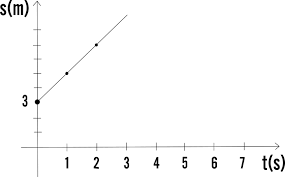
\includegraphics[width=6cm, height=3cm]{diagrammaOrario.png} % Percorso dell'immagine
    \caption{Diagramma Orario} % Didascalia per l'immagine
    \label{fig:immagine} % Etichetta per riferimento
\end{figure}
\subsection{Velocità nel moto rettilineo}
Supponiamo che all'istante $t=t_1$ il punto si trovi nella posizione $x_1$ e all'istante $t=t_2$ nella posizione $x_2$. Lo \textbf{spostamento} del punto nell'intervallo di tempo $\Delta t=t_2-t_1$ è $\Delta x=x_2 - x_1$. La \textbf{velocità media $v_m$} del punto è definita come rapporto tra lo spostamento $\Delta x$ e l'intervallo di tempo $\Delta t$:
\begin{equation}
    v_m=\frac{\Delta x}{\Delta t} = \frac{x_2-x_1}{t_2 - t_1}
\end{equation}
La velocità media, esprime la rapidità con cui avviene lo spostamento. In un generico moto rettilineo la velocità non è costante nel tempo. Definiamo quindi la \textbf{velocità istantanea} di un punto nel moto rettilineo come la derivata dello spazio rispetto al tempo:
\begin{equation}
    v = \frac{dx}{dt}
\end{equation}

La \textbf{velocità istantanea} rappresenta la rapidità di variazione temporale della posizione nell'istante t considerato. Il segno della velocità indica il verso del moto sull'asse x: se $v>0$ la coordinata x cresce, mentre se $v<0$ il moto avviene nel verso opposto. Nel caso particolare in cui v=costante si parla di \textbf{moto rettilineo uniforme}. Nota la \textbf{legge oraria ($x(t)$)} possiamo ottenere la velocità istantanea come la sua derivata. Lo spostamento infinitesimo dx è uguale al prodotto del tempo dt impiegato a percorrerlo per il valore della velocità al tempo t:
\begin{equation}
    dx=v(t)dt
\end{equation}

Considerando $\Delta x = \int_{x_0}^x dx = \int_{t_0}^t v(t) dt$ (grazie alla formula trovata prima di dx) troviamo che (sostituendo $\Delta x$ con $x-x_0$):
\begin{equation}
    x(t)=x_0 + \int_{t_0}^t v(t) dt
\end{equation}
Questa è la relazione generale che permette il calcolo dello spazio percorso nel moto rettilineo, qualunque sia il tipo di moto. Ricordando la definizione di velocità media, $v_m = (x-x_0)/(t-t_0)$ ricaviamo la relazione tra la velocità media e velocità istantanea. Ricordando che $\Delta x = x-x_0=\int_{x_0}^x dx = \int_{t_0}^t v(t) dt$
\begin{equation}
v_m = \frac{1}{t-t_0}\int_{t_0}^t v(t) dt
\end{equation}
Siccome matematicamente questa formula coincide con il \textbf{valor medio di una funzione in un dato intervallo}: pertanto la \textbf{velocità media}, pari al rapporto tra lo spazio complessivamente percorso e il tempo impiegato a percorrerlo, è uguale al valor medio della \textbf{velocità istantanea} nell'intervallo di tempo considerato.
\subsubsection{Moto rettilineo uniforme}
Applicando 1.3.4 considerando il caso particolare del \textbf{moto rettilineo uniforme} in cui $v=costante$.
\begin{equation}
    x(t)= x_0 + v \int_{t_0}^t dt = x_0 + v(t-t_0), \ x(t) = x_0 + vt
\end{equation}
Queste due vengono definite come \textbf{le leggi orarie o equazioni del moto rettilineo uniforme}. Esse mostrano che in questo moto lo spazio è una funzione lineare del tempo: in tempi eguali sono percorsi spazi uguali. La \textbf{velocità istantanea} corrisponde alla velocità media. $a=0$.
\subsection{Accelerazione nel moto rettilineo}
Quando la velocità del punto varia nel tempo il \textbf{moto} si dice \textbf{accelerato}. Se tra gli istanti $t_1$ e $t_2$ la velocità varia da $v_1$ a $v_2$, si definisce \textbf{accelerazione media} del punto il rapporto tra la variazione di velocità $\Delta v$ e l'intervallo di tempo $\Delta t$ in cui avviene la variazione:
\begin{equation}
    a_m = \frac{v_2 - v_1}{t_2 - t_1} = \frac{\Delta v}{\Delta t}
\end{equation}
Definiamo poi l'\textbf{accelerazione istantanea}, cioè la \textbf{rapidità di variazione temporale della velocità}, come:
\begin{equation}
    a=\frac{dv}{dt}=\frac{d^2x}{dt^2}
\end{equation}
L'\textbf{accelerazione istantanea} è dunque la derivata della velocità rispetto al tempo, ovvero la derivata seconda dello spazio rispetto al tempo. Se $a=0$ la velocità è costante. Quando a è positiva la velocità cresce nel tempo mentre per $a<0$ la velocità decresce. 
\begin{equation}
    dv=a(t)dt
\end{equation}
Scriviamo $\Delta v =  \int_{v_0}^v dv=\int_{t_0}^t a(t)dt$ e pertanto
\begin{equation}
    v(t) = v_0 + \int_{t_0}^t a(t)dt
\end{equation}
\subsubsection{Moto rettilineo uniformemente accelerato}
Il moto rettilineo più generale è vario, se l'accelerazione è costante durante il \textbf{moto} questo si dice \textbf{uniformemente accelerato} e la dipendenza della velocità dal tempo è lineare:
\begin{align}
    v(t) &=v_0 + a(t-t_0) \\
    x(t) &= x_0 + v_0(t-t_0)+\frac{1}{2}a(t-t_0)^2 \\
    x(t) &= x_0 + v_0 t + \frac{1}{2}at^2
\end{align}
\newpage
\subsection{Moto verticale di un corpo}
Un corpo lasciato libero di cadere in vicinanza della superficie terrestre si muove verso il basso con un'accelerazione costante $g=9.8ms^{-2}$.
\begin{figure}[H] % Usa 'H' per forzare la posizione qui
    \centering % Centra l'immagine
    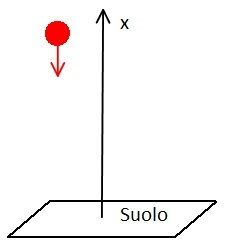
\includegraphics[width=6cm, height=3cm]{Moto_verticale_di_un_corpo.jpg} % Percorso dell'immagine
    \caption{Sistema di riferimento per un moto rettilineo verticale} % Didascalia per l'immagine
    \label{fig:immagine} % Etichetta per riferimento
\end{figure}
\noindent
Il moto osservato sperimentalmente è dunque rettilineo uniformemente accelerato. Esaminiamo alcune possibili situazioni, cominciando dalla caduta libera da un'altezza h con velocità iniziale nulla: le condizioni iniziali sono perciò $x_0=h$ e $v_0=0$ per $t=t_0=0$. Ricorriamo alle \textbf{leggi generali} del moto rettilineo uniformemente accelerato per poter scrivere velocità e posizione in funzione del tempo. 
\begin{equation}
    v(t)=-gt, \ x(t)=h-\frac{1}{2}gt^2
\end{equation}
Considerando $x(t)=0$ perchè sarebbe quando l'oggetto tocca il suolo. Calcoliamo il tempo di caduta e la velocità al suolo (in modulo) come:
\begin{equation}
    t_c=\sqrt{\frac{2h}{g}}, \ v_c=\sqrt{2gh}
\end{equation}
Se invece il punto è lanciato verso il basso (condizioni iniziali $x_0=h$ e $v_0=-v_1$), si trovano le seguenti espressioni
\begin{equation}
    v(t)=-v_1 -gt, \ x(t)=h-v_1t-\frac{1}{2}gt^2
\end{equation}
\begin{equation}
    t_c=\frac{-v_1}{g}+\sqrt{\frac{{v_1}^2}{g^2}+\frac{2h}{g}}, \ v_c=\sqrt{ v_1^2 - 2gh}
\end{equation}
Osserviamo che $t_c$ risulta minore di quello calcolato nella situazione precedente proprio perchè il punto possiede una velocità iniziale rivolta verso il basso. Per la stessa ragione $v_c$ risulta maggiore. Ponendo $v_1=0$ ovviamente si ritrovano i risultati visti prima. Infine se il punto viene lanciato verso l'alto, con velocità $v_2$, ma partendo dal suolo, le condizioni iniziali sono $x_0=0$ e $v_0=v_2>0$ per $t=0$.
\begin{equation}
    v(t)=v_2 -gt, \ x(t)=v_2t-\frac{1}{2}gt^2
\end{equation}
Il punto inizialmente sale verso l'alto (guarda pag 16) con velocità che decresce progressivamente: esso si ferma cioè ha una velocità nulla nell'istante $t_M=v_2/g$ e nella posizione $x_M=x(t_M)=v^2/2g$. Per $t>=t_M$ siamo nella stessa situazione del primo esempio. In conclusione abbiamo usato le due \textbf{leggi generali}:
\begin{equation}
    v(t)=v_0 -gt, \ x(t)=x_0 + v_0t-\frac{1}{2}gt^2
\end{equation}
\subsection{Moto Armonico Semplice}
Un punto esegue un \textbf{moto armonico semplice} quando la legge oraria è definita dalla relazione:
\begin{equation}
    x(t)=A\sin({\omega t + \phi})
\end{equation}
A è detta \textbf{ampiezza del moto}, $\omega t + \phi$ \textbf{fase del moto}, $\phi$ \textbf{fase iniziale}, $\omega$ \textbf{pulsazione}. Dunque il moto armonico semplice è un \textbf{moto vario}, in cui tutte le grandezze cinematiche che lo descrivono: $x(t),v(t), a(t)$ variano nel tempo. Quindi un punto che obbedisce alla seguente legge oraria, percorre un segmento di ampiezza pari a 2A con centro nell'origine. Al tempo $t=0$ il punto occupa la posizione $x(0)=A\sin\phi$: note le costanti A e $\phi$, possiamo determinare la posizione iniziale del punto (solo se $\phi=0$ 0 $\phi=\pi$ il punto è nell'origine per t=0). Il moto armonico, considerando che la funzione seno è periodica con periodo $2\pi$, risulta essere periodico: le oscillazioni di ampiezza A sono caratterizzate dalla durata detta \textbf{periodo} T del modo armonico. Definizione generale: il moto di un punto si dice \textbf{periodico} quando ad intervalli di tempo eguali il punto ripassa nella stessa posizione con la stessa velocità.
\begin{equation}
    T=\frac{2\pi}{\omega} \ ovvero \ \omega=\frac{2\pi}{T}
\end{equation}
Capiamo cosi il significato di $\omega$: il moto si ripete velocemente quando la pulsazione è grande mentre il moto è lento per bassi valori della pulsazione. Si definisce \textbf{frequenza} $\nu$ del moto il numero di oscillazioni in un secondo:
\begin{equation}
    \nu = \frac{1}{T}=\frac{\omega}{2\pi}
\end{equation}
Fissato il valore della pulsazione abbiamo una classe di moti armonici, caratterizzati dallo stesso periodo, che differiscono tra loro per i diversi valori dell'ampiezza e della fase iniziale, cioè, come vedremo, per le diverse condizioni iniziali.
\begin{equation}
    v(t)=\frac{dx}{dt}=\omega Acos(\omega t+ \phi)
\end{equation}
\begin{equation}
    a(t)=\frac{dv}{dt}=\frac{d^2x}{dt^2}=-\omega^2Asen(\omega t + \phi) = -\omega^2 x(t)
\end{equation}
\begin{figure}[H] % Usa 'H' per forzare la posizione qui
    \centering % Centra l'immagine
    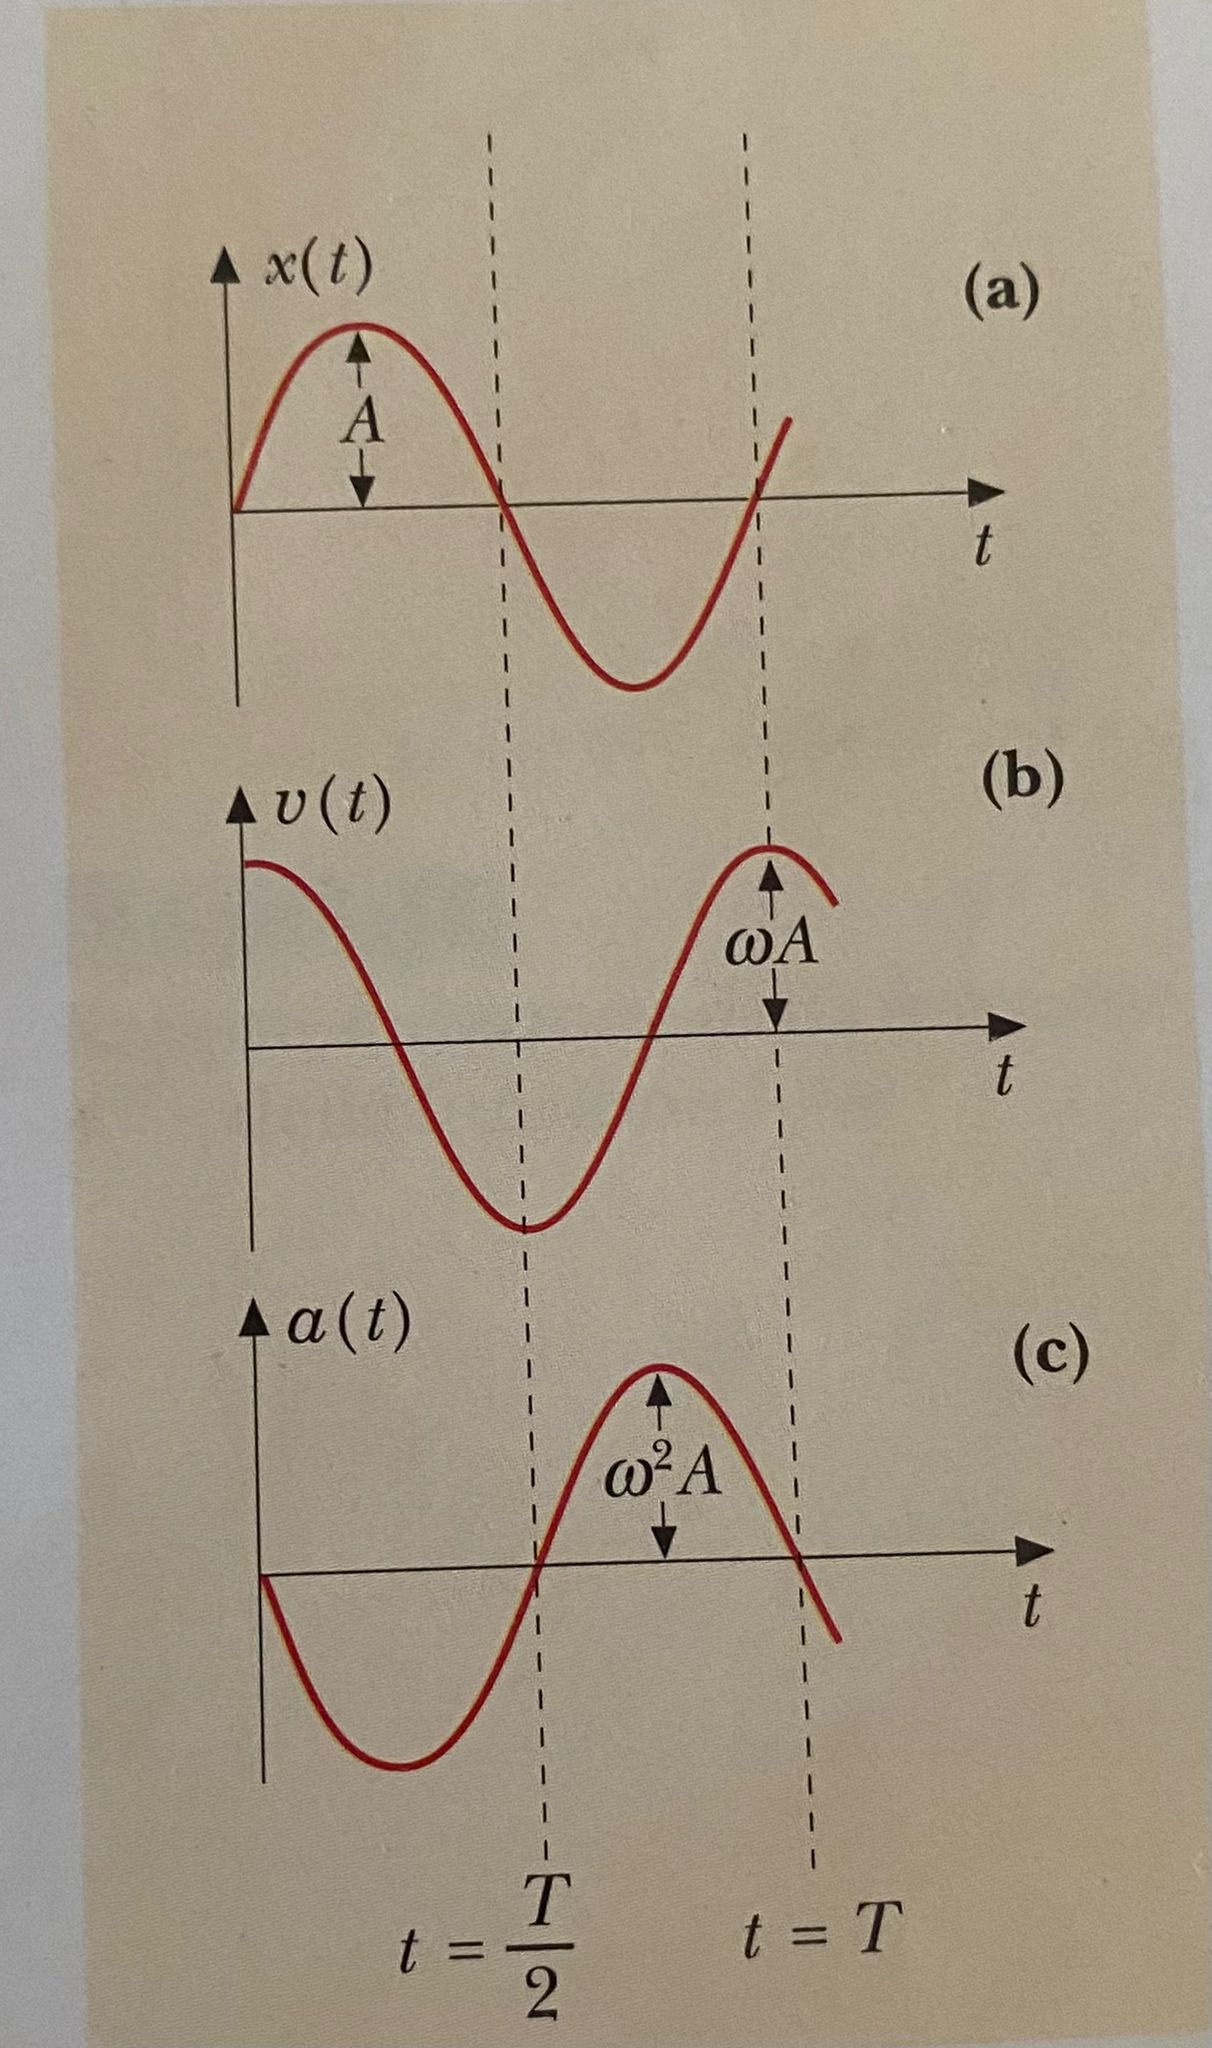
\includegraphics[width=3cm, height=4cm]{MotoArmonicoSemplice.jpg} % Percorso dell'immagine
    \caption{Diagramma dello spostamento (a), della velocità (b) e dell'accelerazione (c) di un moto armonico semplice} % Didascalia per l'immagine
    \label{fig:immagine} % Etichetta per riferimento
\end{figure}
\noindent
La velocità assume il valore massimo nel centro di oscillazione dove vale $\omega A$ e si annulla agli estremi ($x=A \ e \ x=-A$) dove si inverte il senso del moto. L'accelerazione si annulla nel centro di oscillazione e assume il valore massimo in modulo ($\omega^2A$) agli estremi, dove si inverte la velocità. In particolare la velocità è sfasata di $\frac{\pi}{2}$ rispetto allo spostamento (è in quadratura di fase), mentre l'accelerazione è sfasata di $\pi$ sempre rispetto allo spostamento (è in opposizione di fase). Le costanti A e $\phi$ individuano le condizioni iniziali:
\begin{equation}
    x(0) = x_0 = Asen\phi \ , \ v(0) = v_0 = \omega A cos \phi
\end{equation}
Viceversa, note le condizioni iniziali $x_0$ e $v_0$ si calcolano A e $\phi$:
\begin{equation}
    tg\phi = \frac{\omega x_0}{v_0}
\end{equation}
\begin{equation}
    A^2=x_0^2 + \frac{v_0^2}{\omega^2}
\end{equation}
La condizione necessaria e sufficiente perchè un moto sia armonico è data dall'equazione:
\begin{equation}
    \frac{d^2x(t)}{dx^2} + \omega^2x(t)=0
\end{equation}
detta del moto armonico.
\subsection{Moto Rettilineo Smorzato Esponenzialmente}
Viene considerato un caso particolare di moto \textbf{vario}, in cui l'accelerazione soddisfa alla condizione $a=-kv$, con k costante positiva. Di conseguenza l'accelerazione in questo moto è sempre contraria alla velocità che perciò deve necessariamente diminuire, e varia con la stessa legge con cui varia la velocità. Arrivando a determinare la \textbf{velocità} come:
\begin{equation}
    v(t)=v_0e^{-kt}
\end{equation}
Dove $v_0$ deve necessariamente essere diverso da 0 dato che così sia la velocità che l'accelerazione sarebbero uguali a 0 e non ci sarebbe moto. Per quanto riguarda la \textbf{legge oraria}:
\begin{equation}
    x(t)=\frac{v_0}{k}(1-e^{-kt})
\end{equation}
\begin{figure}[H] % Usa 'H' per forzare la posizione qui
    \centering % Centra l'immagine
    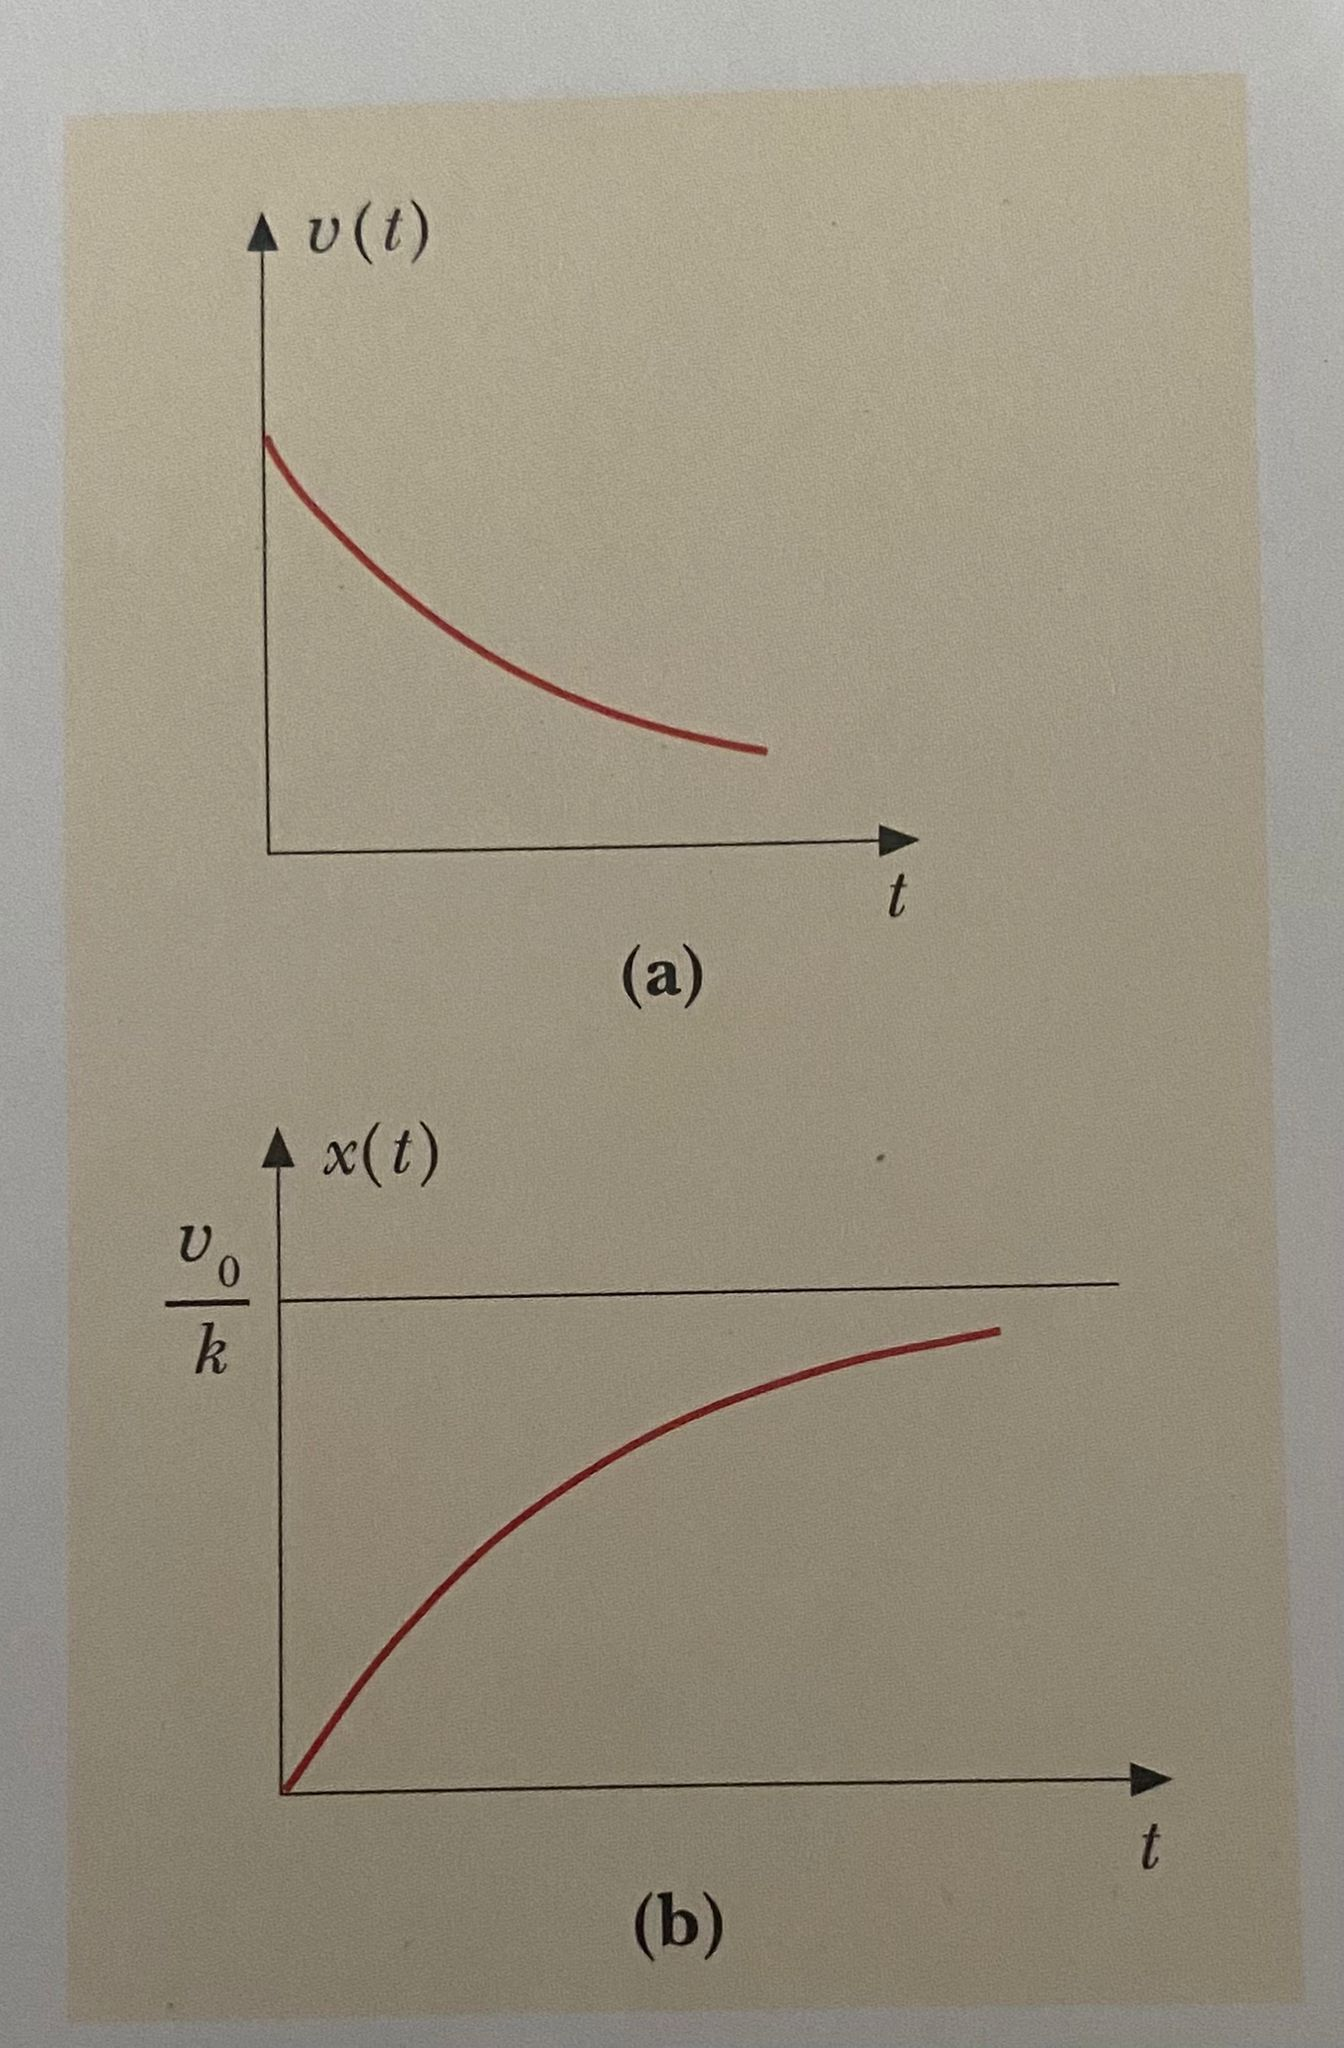
\includegraphics[width=4cm, height=5cm]{MotoRettilineoSmorzatoEsponenzialmente.jpg} % Percorso dell'immagine
    \caption{Diagramma della velocità (a) e dello spostamento (b) di un punto soggetto ad una accelerazione a=-kv} % Didascalia per l'immagine
    \label{fig:immagine} % Etichetta per riferimento
\end{figure}
\noindent
Il punto tende asintoticamente alla posizione $v_0/k$. Osserviamo che la rapidità di variazione della funzione $e^{-kt}$ è determinata dal valore di k. Introduciamo poi $\tau$ che si chiama \textbf{costante di tempo} e si misura in secondi.
\subsection{Velocità e Accelerazione in funzione della posizione}
Vi sono delle situazioni fisiche, in cui la variabile tempo, non compare esplicitamente: per esempio quando l'accelerazione è nota in funzione della posizione. Supponiamo pertanto di conoscere la funzione a(x) e vediamo come da questa informazione sia possibile ricavare la funzione v(x). Troviamo che:
\begin{equation}
    \int_{x_0}^x a(t)dx=\frac{1}{2}v^2-\frac{1}{2}v_0^2
\end{equation}
Così è possibile calcolare la variazione del modulo della velocità in corrispondenza ad un percorso finito lungo cui sia nota $a(x)$, anche senza conoscere la legge oraria.
Dove $v_0$ è la velocità del punto in $x_0$. Applichiamo adesso ai vari casi:
\subsubsection{Moto uniformemente accelerato (1.4)}
L'accelerazione è una funzione costante, in ogni istante e in ogni posizione; si ha subito:
\begin{equation}
    v^2(x)=v_0^2 + 2a(x-x_0)
\end{equation}
\subsubsection{Caduta di un corpo (1.5)}
\textbf{Caduta libera da un'altezza h con $v_0=0$}:
\begin{equation}
    v(x)=\sqrt{2g(h-x)}
\end{equation}
\textbf{Punto lanciato verso il basso}
\begin{equation}
    v(x)=\sqrt{v_1^2+2g(h-x)}
\end{equation}
\textbf{Punto lanciato verso l'alto}
\begin{equation}
    v(x)=+-\sqrt{v_2^2-2gx}
\end{equation}
Il doppio segno dell'ultima formula deriva dal fatto che il punto passa due volte nella stessa posizione, una volta salendo (segno positivo) e una volta scendendo (segno negativo). In particolare $x=0$ è occupato alla partenza ($t=0,v=v_2$) e all'arrivo ($t=2t_M, v=-v_2$): il punto ritorna nell'origine con velocità eguale in modulo a quella di partenza, ma ovviamente di segno opposto.
\subsubsection{Moto Armonico Semplice (1.6)}
La 1.6.5 fornisce la dipendenza dell'accelerazione da x: a varia linearmente con la distanza dal centro di oscillazione ed è di segno opposto ad essa. 
\begin{equation}
    v^2(x)=v_0^2+\omega^2(x_0^2-x^2)
\end{equation}
\subsubsection{Moto Smorzato Esponenzialmente}
\begin{equation}
    v(x)=v_0-k(x-x_0)
\end{equation}
La velocità decresce linearmente con la distanza percorsa e in particolare il punto si ferma ($v=0$) nella posizione $x-x_0=\frac{v_0}{k}$.
\subsection{Moto Relativo Rettilineo}
Se due punti $P_1 \ e \ P_2$ si muovono lungo l'asse x, il primo con legge oraria $x_1(t)$ e il secondo con legge oraria $x_2(t)$, la \textbf{posizione relativa} di $P_2$ rispetto a $P_1$ è data da:
\begin{equation}
    x_{1,2}=x_2(t)-x_1(t)
\end{equation}
La funzione $x_{1,2}(t)$ fornisce la legge oraria del \textbf{moto relativo} di $P_2$ rispetto a $P_1$, ovvero del moto di $P_2$ visto da un osservatore solidale con il punto $P_1$. La variazione nel tempo della distanza corrisponde alla \textbf{velocità relativa} di $P_2$ rispetto a $P_1$:
\begin{equation}
    v_{1,2}(t)= v_2(t)-v_1(t)
\end{equation}
Analogamente l'\textbf{accelerazione relativa} di $P_2$ rispetto a $P_1$:
\begin{equation}
    a_{1,2}(t)= a_2(t)-a_1(t)
\end{equation}
Qualora si considerasse il moto di $P_1$ rispetto a $P_2$ sarebbero valide le stesse espressioni col segno cambiato:
\begin{equation}
    x_{2,1}(t)=-x_{1,2}(t), \ v_{2,1}(t)=-v_{1,2}(t), \ a_{2,1}(t)=-a_{1,2}(t)
\end{equation}
Nota $a_{1,2}(t)$ e $v_{1,2}(0)$, velocità relativa iniziale, si calcola:
\begin{equation}
    v_{1,2}(t)=v_{1,2}(0) + \int_0^t a_{1,2}(t)dt
\end{equation}
di qui nota la posizione relativa iniziale $x_{1,2}(0)$, si ha:
\begin{equation}
    x_{1,2}(t)=x_{1,2}(0) + \int_0^t v_{1,2}(t)dt
\end{equation}
Il moto relativo è \textbf{uniforme} se $a_{1,2}(t)=0$, ovvero se $a_1(t)=a_2(t)$, è \textbf{uniformemente accelerato} se $a_{1,2}$ è costante, è vario se $a_{1,2}$ varia nel tempo. Non c'è moto relativo se le velocità dei due punti sono eguali.
\section{Calcolo Vettoriale}
\subsection{Grandezze scalari e vettoriali}
Le grandezze per cui la rappresentazione basta un solo numero, costante o funzione delle coordinate ed eventualmente anche del tempo, si dicono \textbf{grandezze scalari}. Le operazioni che si eseguono su di esse obbediscono alle solite regole dell'algebra. Nel testo sono indicate in \textbf{carattere corsivo}. Ci sono però situazioni in cui un solo numero non è sufficiente \\
\begin{center}
    \begin{tikzpicture}
  \draw[->, thick] (0,0) -- (3,2) node[above] {$\vec{v}$};
\end{tikzpicture} \\
\end{center}
Come ad esempio uno spostamento. Esistono dunque grandezze che per essere specificate hanno bisogno di un numero, il \textbf{modulo}, che ne da il valore assoluto, di una \textbf{direzione} e di un \textbf{verso}. Il \textbf{vettore} è l'ente matematico adatto alla rappresentazione di queste \textbf{grandezze} che si chiamano appunto \textbf{vettoriali} e per le quali vale un'algebra che non è identica all'algebra scalare. Quando due vettori sono eguali possiamo indicarli semplicemente con =. Matematicamente, un vettore ha infinite rappresentazioni: infatti tutti i segmenti orientati di eguale lunghezza, paralleli ed equiversi sono rappresentazioni dello stesso vettore e quindi equivalenti. Si dice che essi formano un sistema di \textbf{vettori equipollenti}.
\subsection{Prime proprietà dei vettori}
La prima operazione che definiamo per i vettori è il \textbf{prodotto di un vettore per uno scalare} (numero) = 
\begin{equation}
    \vec{b}=m\vec{a}
\end{equation}
\begin{figure}[H] % Usa 'H' per forzare la posizione qui
    \centering % Centra l'immagine
    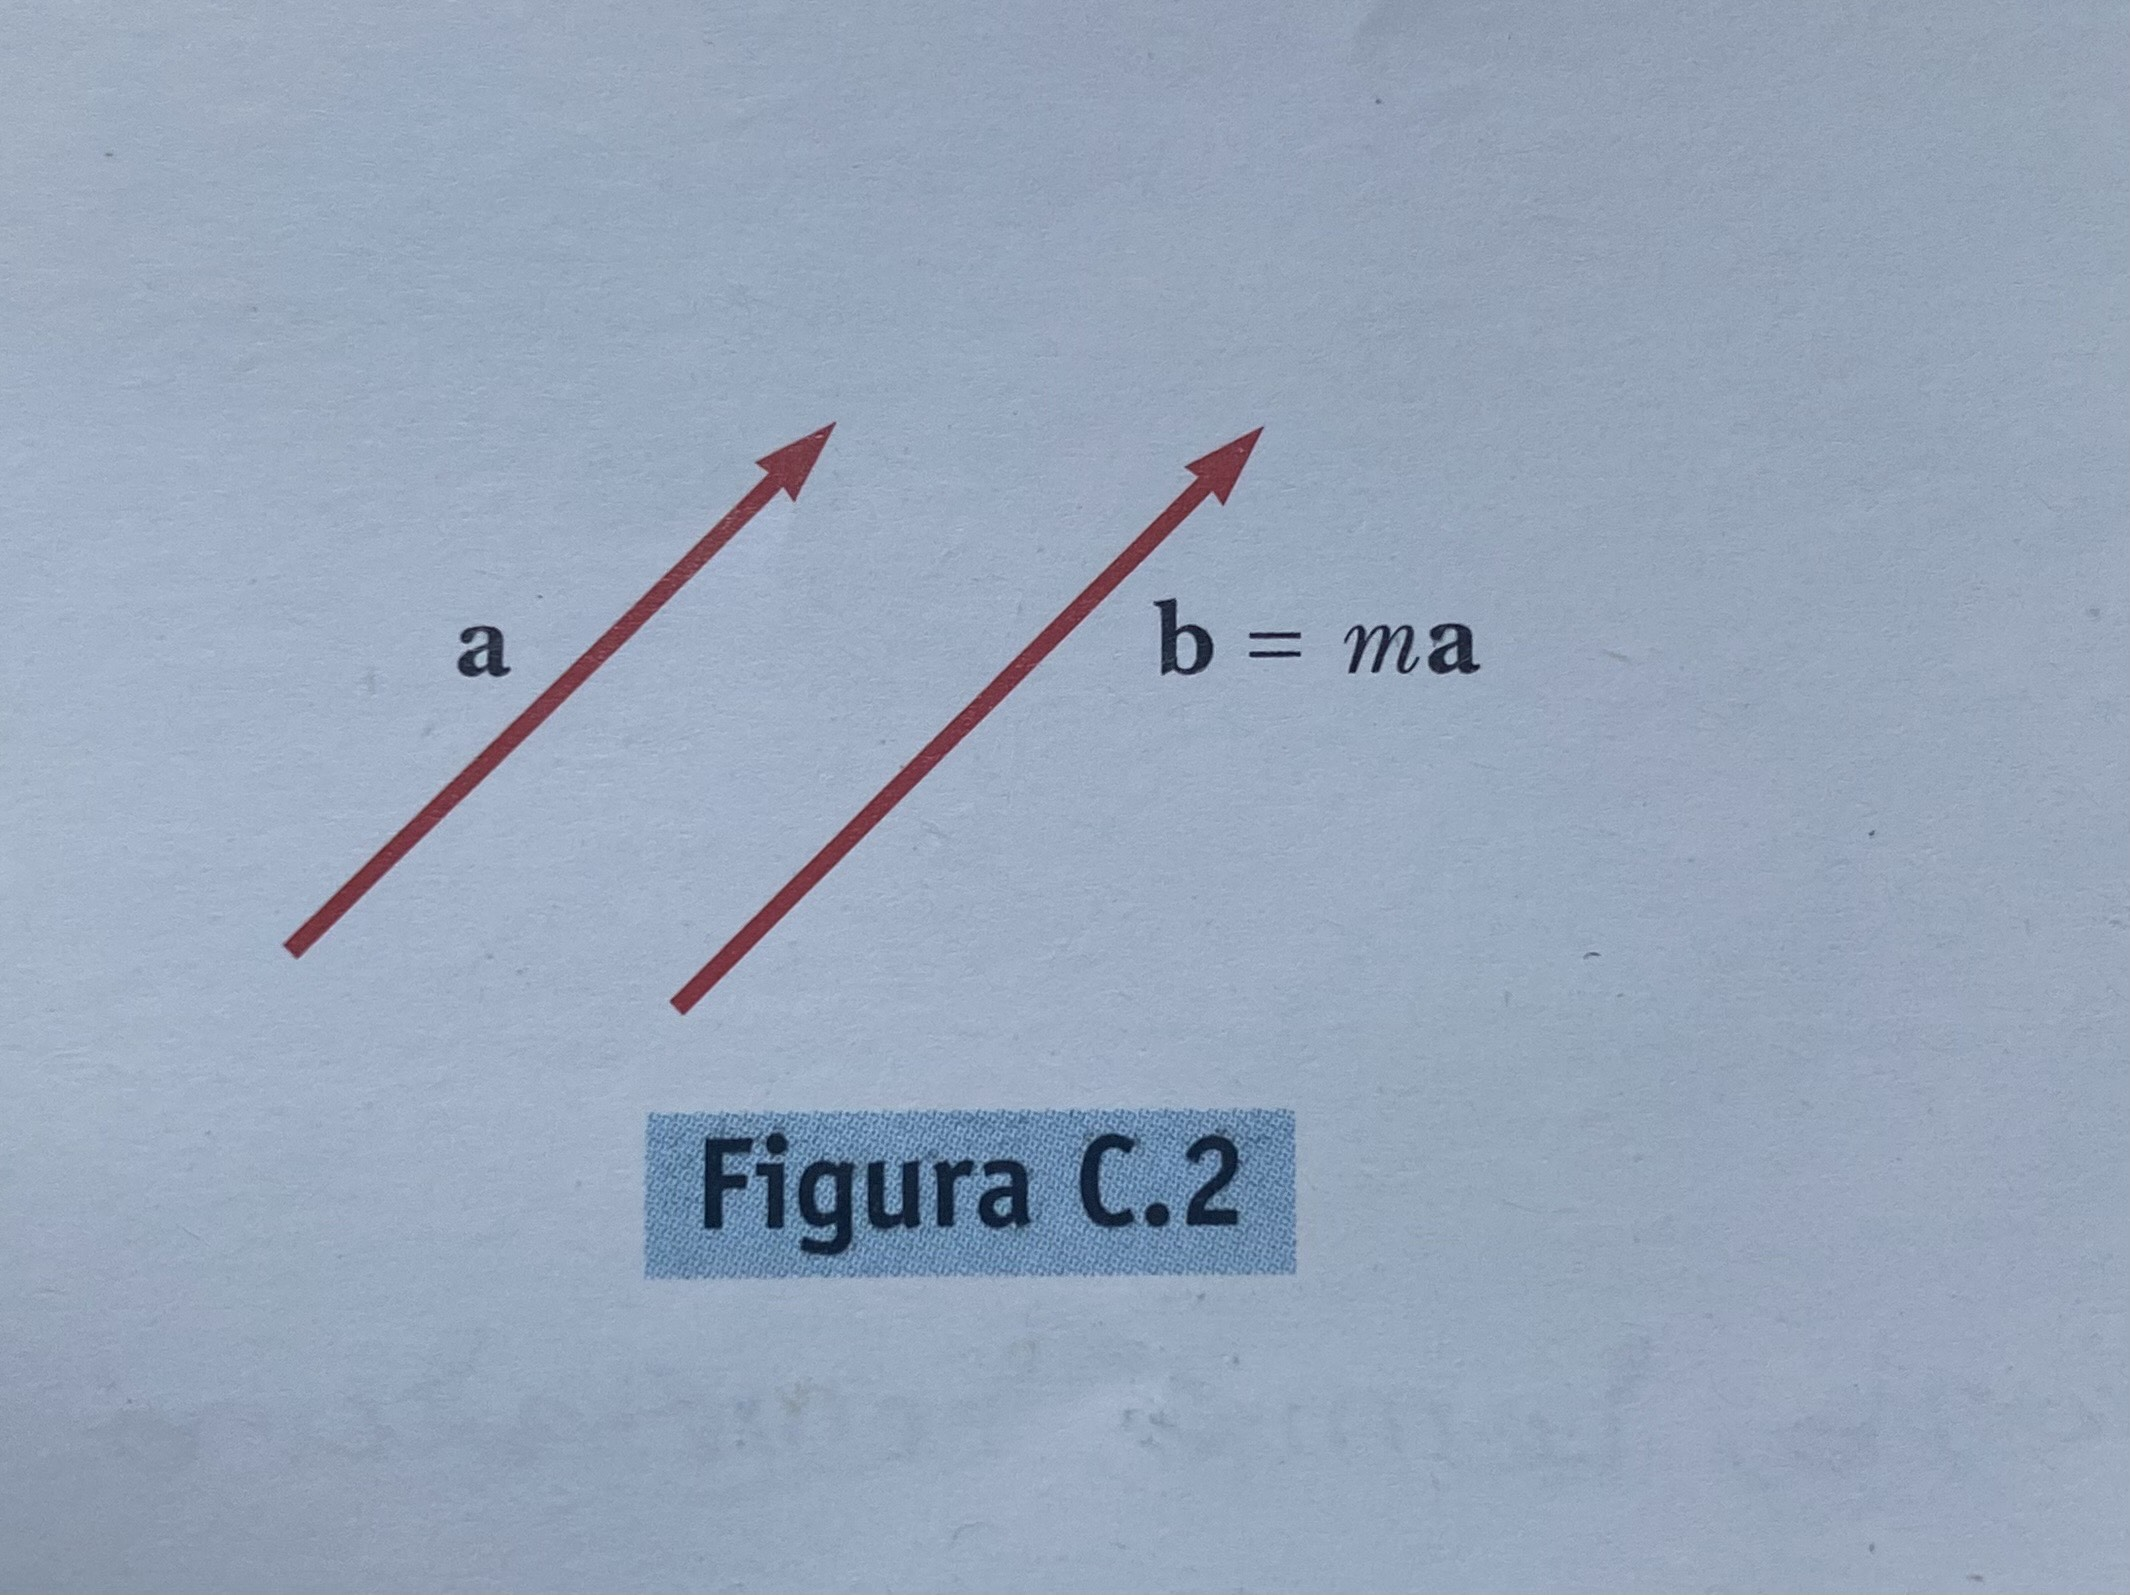
\includegraphics[width=4cm, height=4cm]{ProdottoPerUnoScalare.jpeg} % Percorso dell'immagine
    \caption{} % Didascalia per l'immagine
    \label{fig:immagine} % Etichetta per riferimento
\end{figure}
\noindent
Il prodotto dello scalare m per il vettore $\vec{a}$, ha come risultato un altro vettore $\vec{b}$ che ha la stessa direzione di $\vec{a}$, il modulo m volte quello di a, lo stesso verso di a se $m>0$ e verso opposto se $m<0$. Infatti ponendo $m=-1$ otteniamo il \textbf{vettore opposto} che ha la stessa direzione di a stesso modulo di a ma verso opposto. L'operazione prodotto per uno scalare, porta a un concetto molto importante: fissata una direzione orientata r vi sono infiniti vettori che hanno quella direzione e differiscono solo nel modulo e nel verso. In particolare tra questi esiste il vettore \textbf{u} che è concorde in verso con r e ha modulo unitario. Tutti gli infiniti vettori di cui sopra possono allora scriversi:
\begin{equation}
    \vec{a}=a\vec{u}
\end{equation}
In questa formulazione u descrive la direzione di a, mentre a con il suo segno ne determina il verso, concorde o discorde a u, e con il suo modulo il valore. Il \textbf{vettore unitario u} si chiama il \textbf{versore} della direzione orientata r e per ricordare questo fatto si usa scrivere $\vec{u_r}$.
\newpage
\subsubsection{Regola di somma}
Dati due vettori a e b, in cui b è applicato nel punto terminale di a, la \textbf{somma} è un vettore che si indica con $c=a+b$ e si ottiene graficamente unendo l'origine del vettore a con l'estremo del vettore b.
\begin{figure}[H] % Usa 'H' per forzare la posizione qui
    \centering % Centra l'immagine
    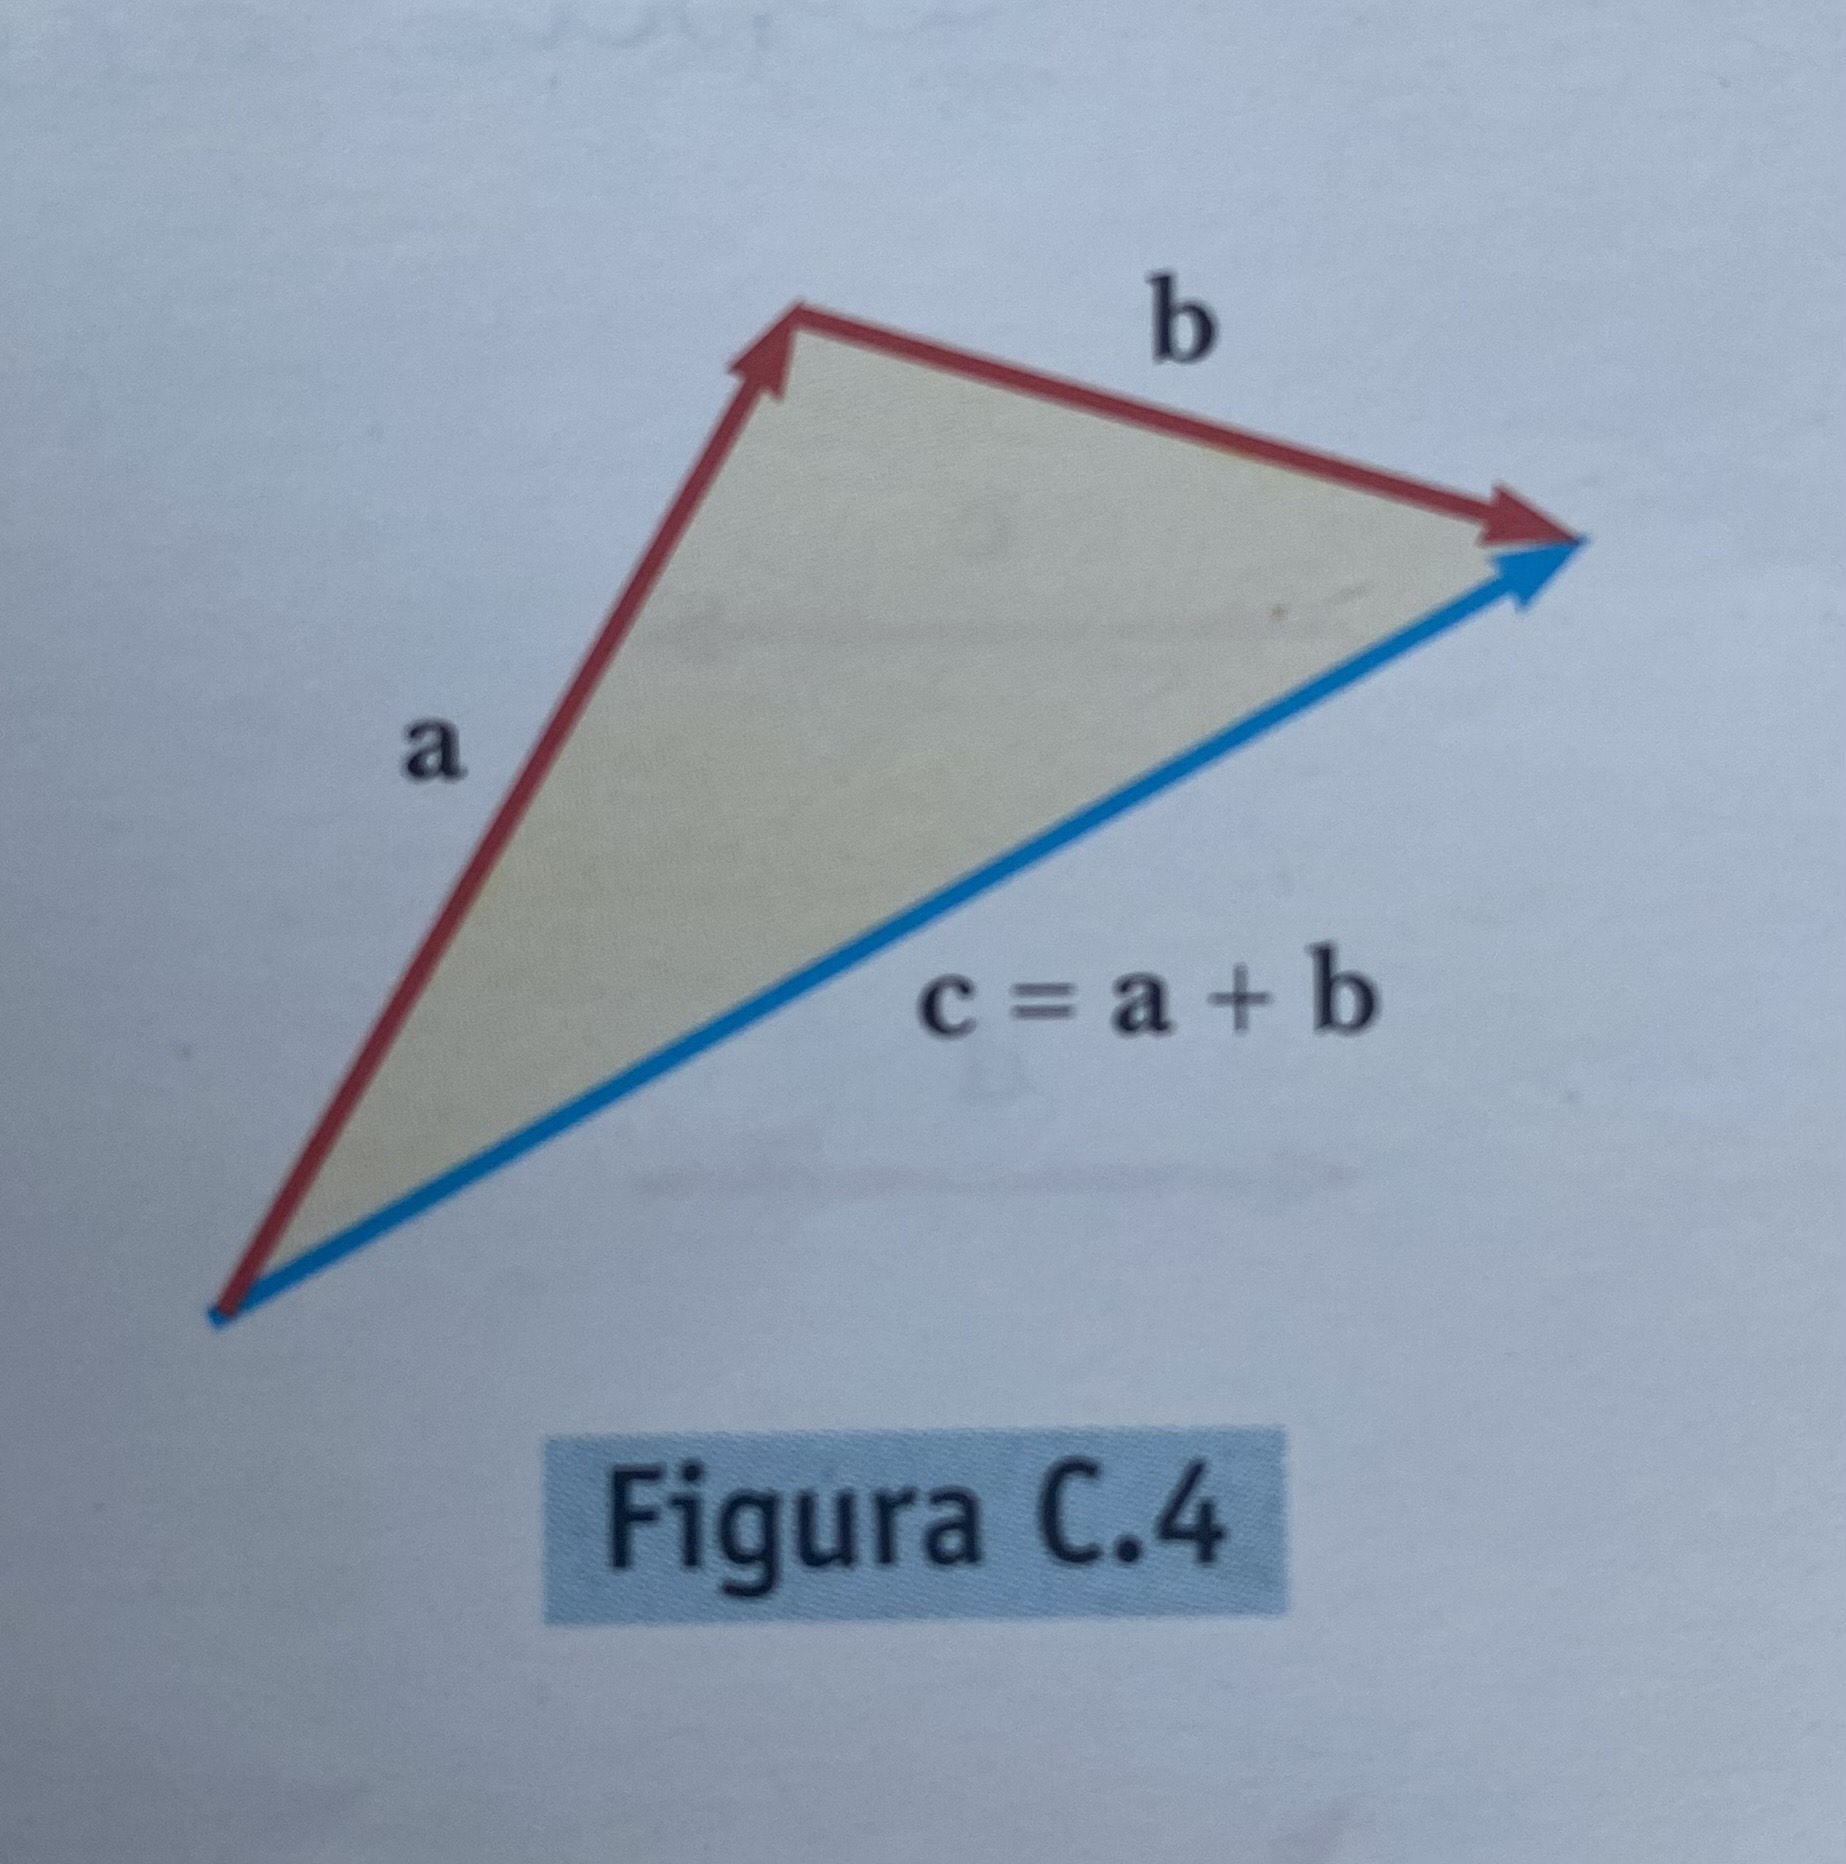
\includegraphics[width=4cm, height=4cm]{RegolaDiSomma.jpeg} % Percorso dell'immagine
    \caption{} % Didascalia per l'immagine
    \label{fig:immagine} % Etichetta per riferimento
\end{figure}
\noindent
Un metodo alternativo per determinare graficamente la somma di due vettori a e b detta \textbf{vettore somma} o \textbf{vettore risultante}, è il cosiddetto \textbf{metodo del parallelogramma}: si applica nell'origine di a anche il vettore b spostandolo parallelamente a se stesso. Il vettore somma $c=a+b$ coincide con la diagonale del parallelogramma, definendo la somma come una proprietà commutativa.
\begin{figure}[H] % Usa 'H' per forzare la posizione qui
    \centering % Centra l'immagine
    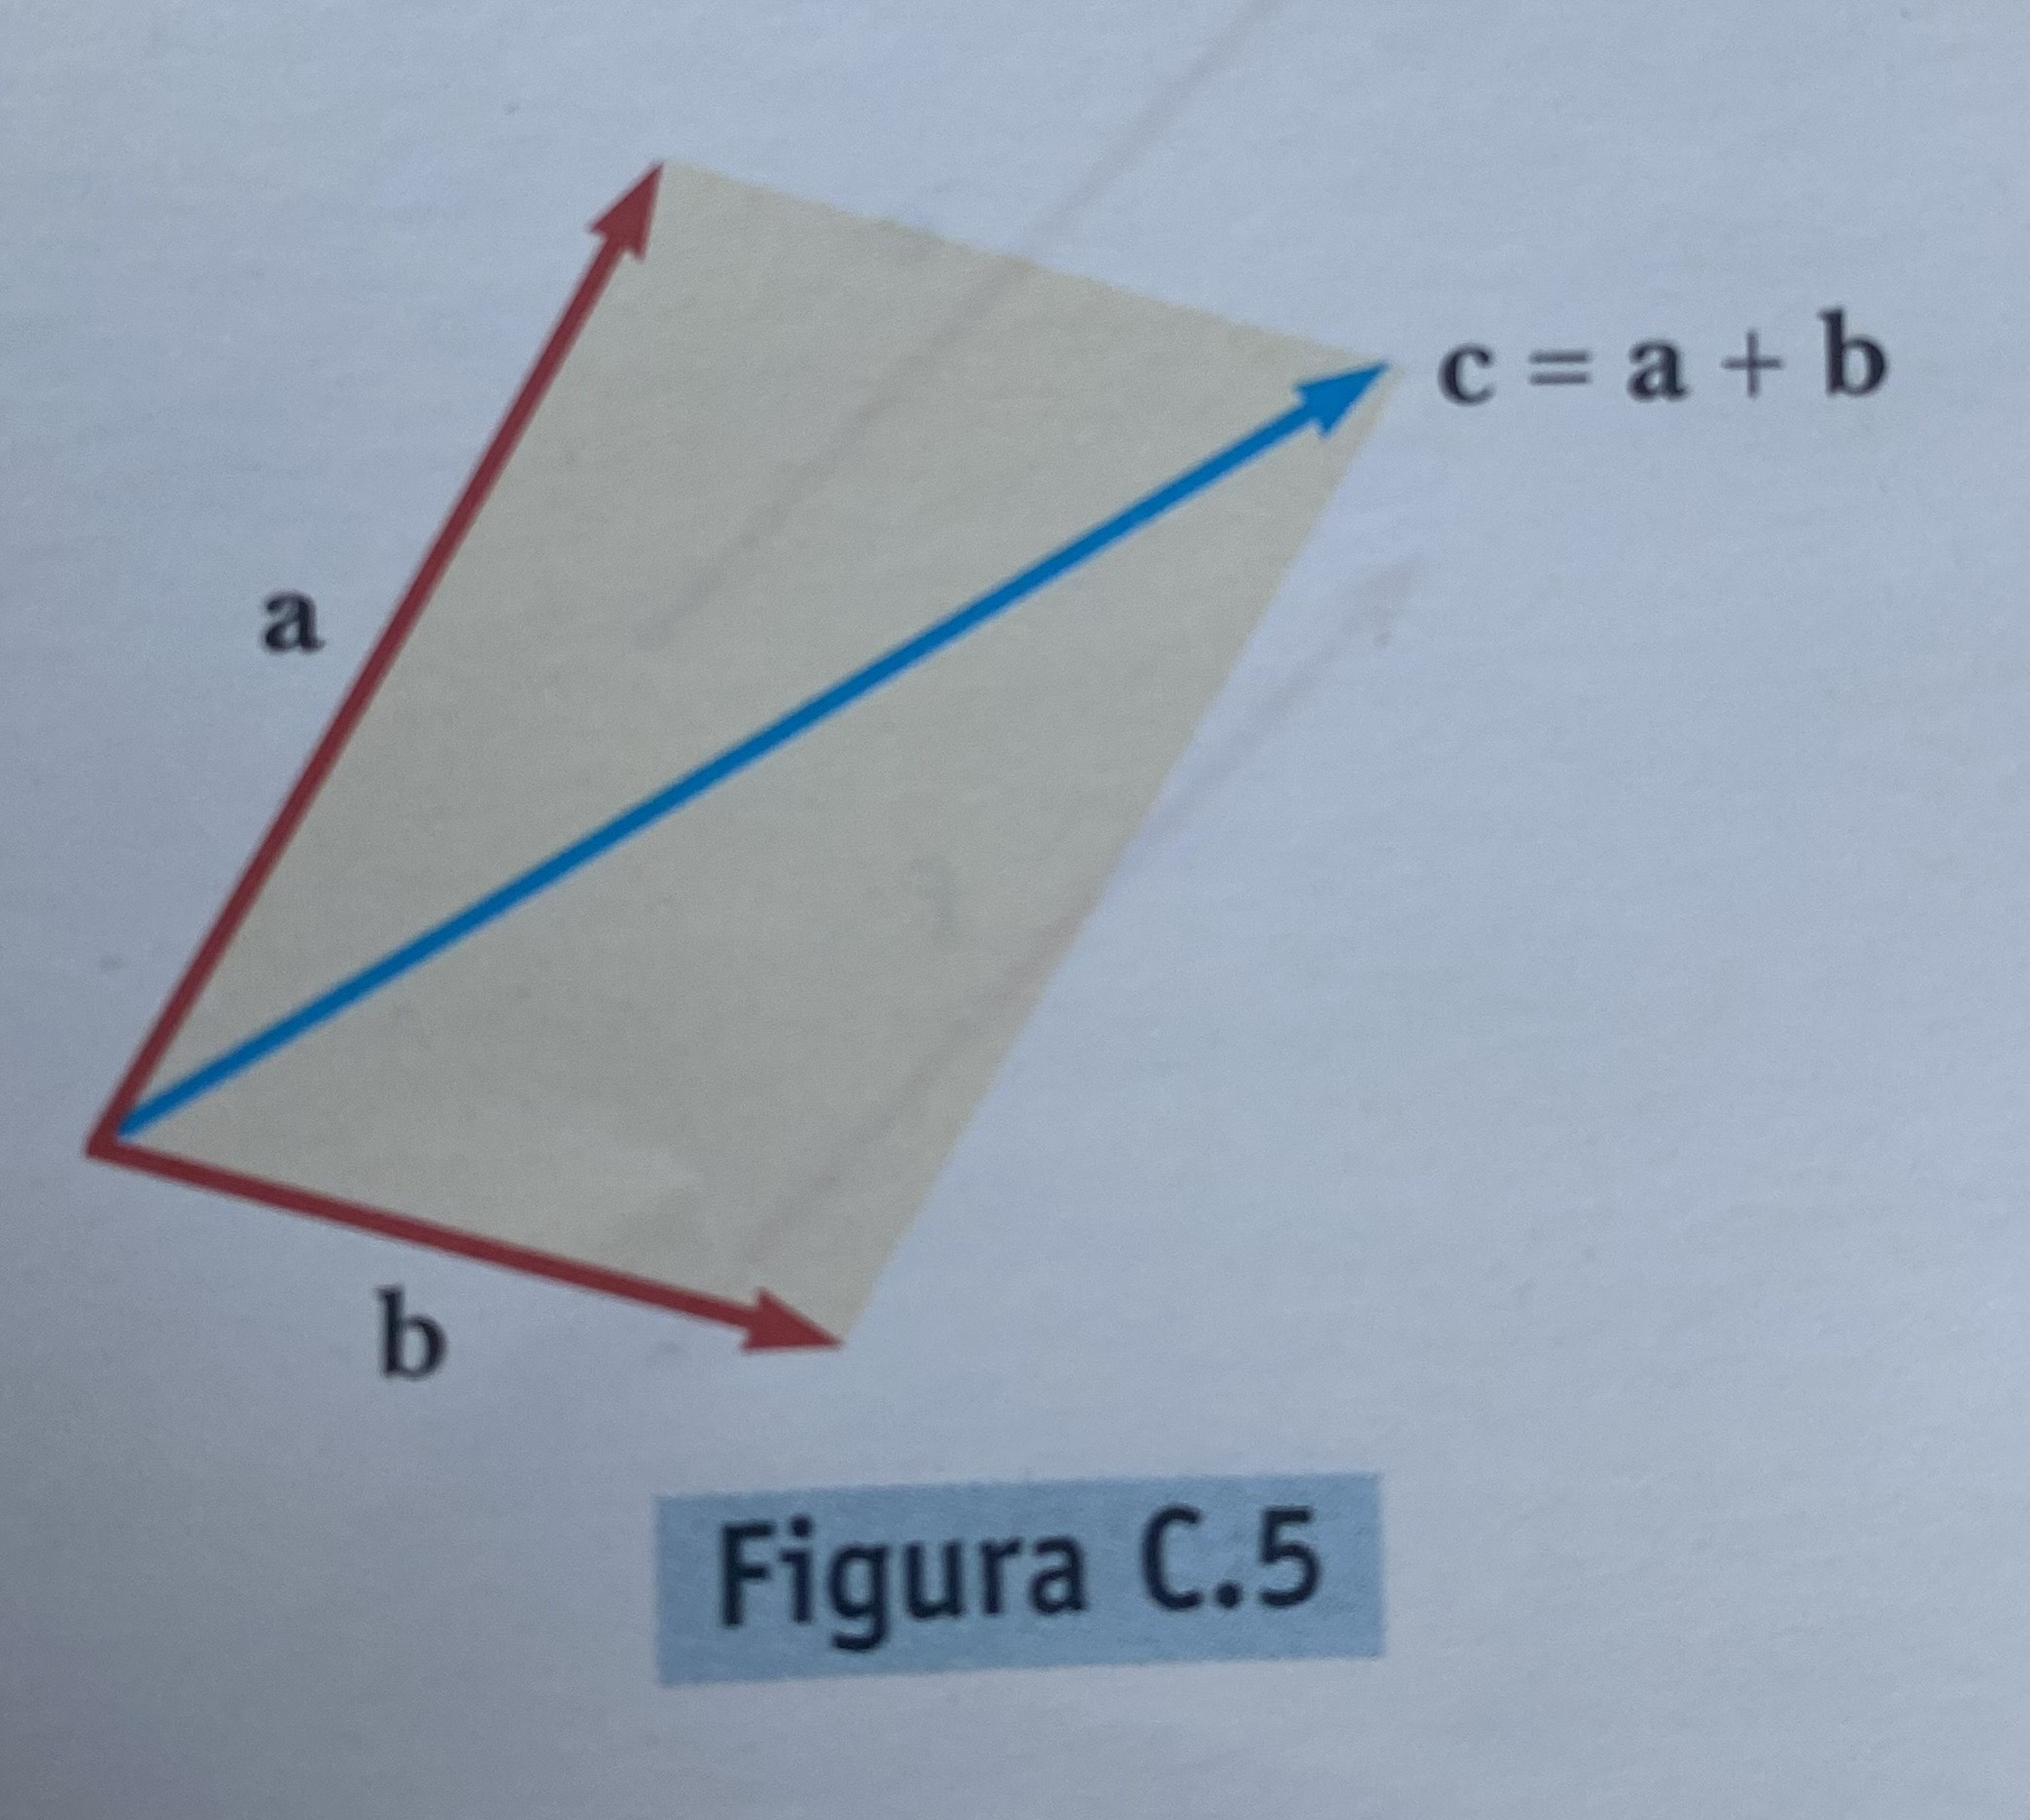
\includegraphics[width=4cm, height=4cm]{RegolaDelPArallelogramma.jpeg} % Percorso dell'immagine
    \caption{} % Didascalia per l'immagine
    \label{fig:immagine} % Etichetta per riferimento
\end{figure}
\noindent
Tramite il concetto di vettore opposto e la regola di somma, si definisce anche la \textbf{differenza di due vettori}:
\begin{equation}
    a-b=a+(-b)
\end{equation}
La regola di somma si estende alla somma di più vettori:
\begin{equation}
    R=a+b+c+d
\end{equation}
Si costruisce così una linea spezzata e il vettore somma R si ottiene congiungendo i due estremi di questa linea. Per la somma vale la \textbf{proprietà associativa}. Nel caso di vettori paralleli, si ha:
\begin{equation}
    a_1+a_2=a_1u+a_2u=(a_1+a_2)u
\end{equation}
\subsubsection{Scomposizione di un vettore}
Consideriamo un vettore v e due direzioni orientate r e s, caratterizzate rispettivamente dai versori $u_r$ e $u_s$. Vogliamo scomporre il vettore v nella somma di due vettori, uno $v_r$ parallelo a $u_r$ e l'altro $v_s$ parallelo a $u_s$, tali che:
\begin{equation}
    v=v_r+v_s=v_ru_r+v_su_s
\end{equation}
\textbf{$v_r$ e $v_s$} si chiamano i \textbf{vettori componenti} del vettore v lungo r e s.
\begin{figure}[H] % Usa 'H' per forzare la posizione qui
    \centering % Centra l'immagine
    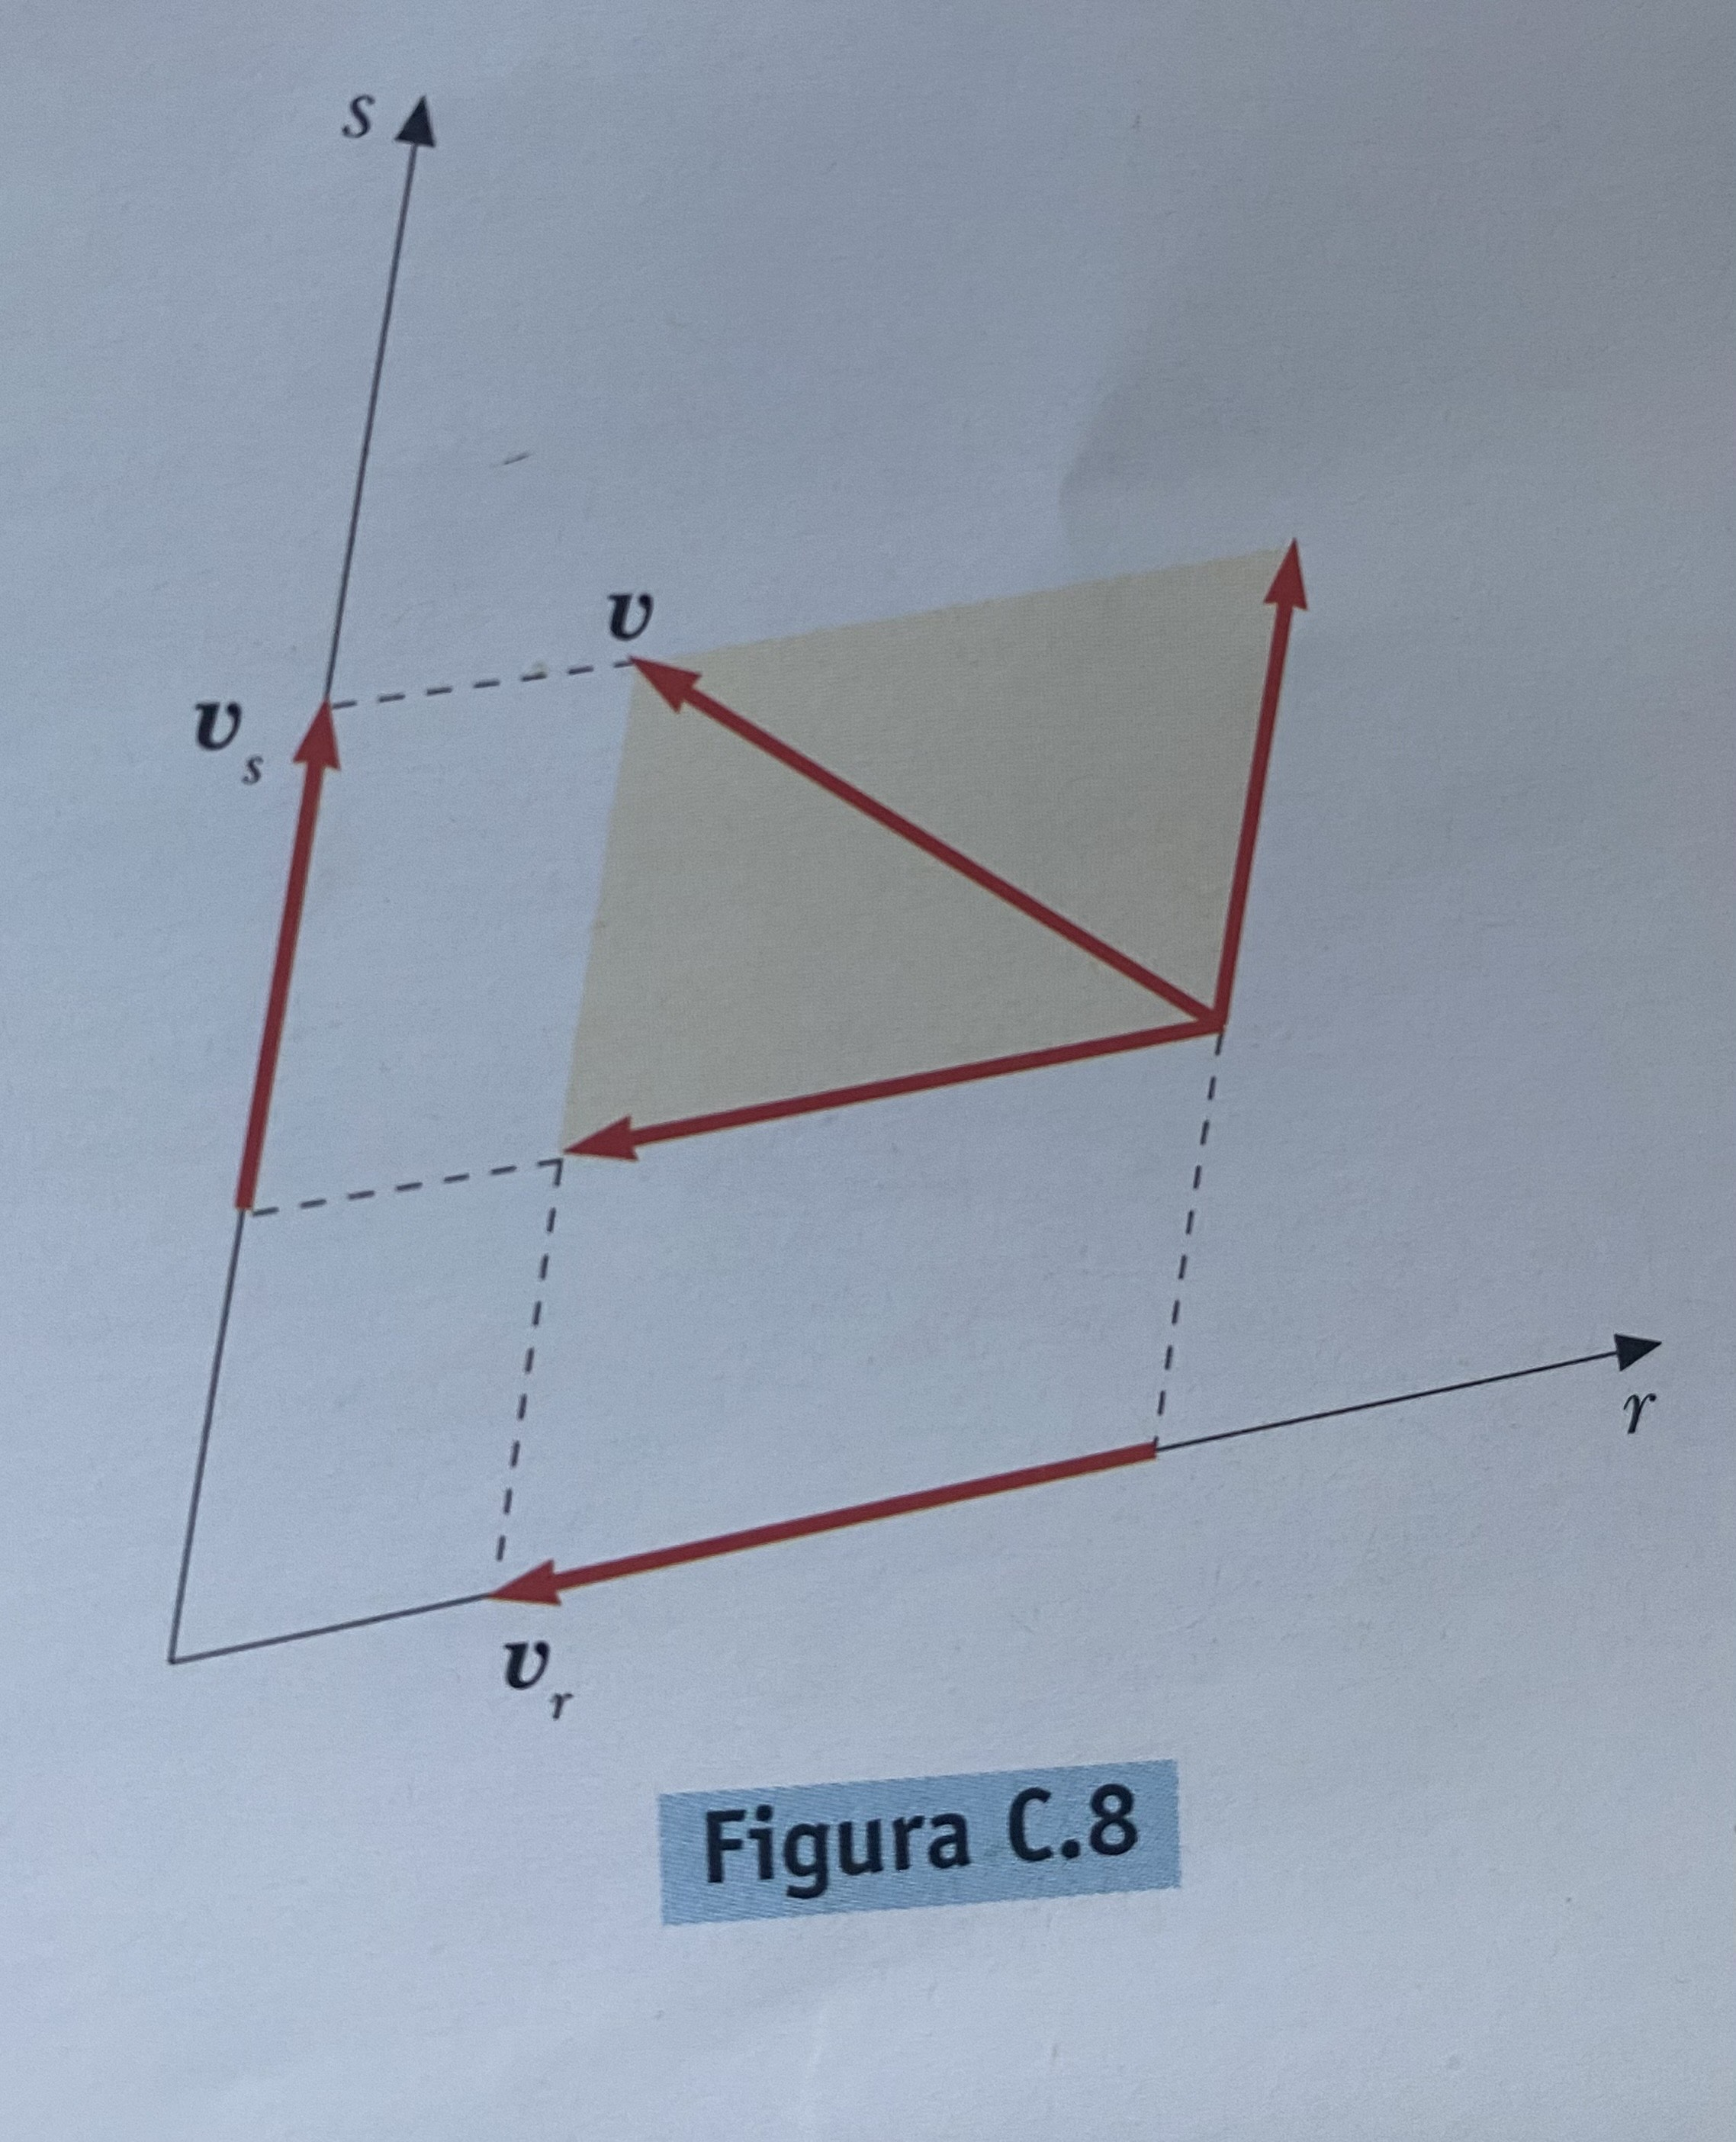
\includegraphics[width=4cm, height=4cm]{ScomposizioneDiUnVettoreSuDIUnPiano.jpeg} % Percorso dell'immagine
    \caption{} % Didascalia per l'immagine
    \label{fig:immagine} % Etichetta per riferimento
\end{figure}
\noindent
Dalla scomposizione lungo due direzioni $u_r$ e $u_s$ che individuano un piano si passa alla scomposizione secondo tre direzioni, nello spazio caratterizzate dai versori $u_r,u_s,u_t$. Il caso di gran lunga più frequente è che le tre direzioni siano gli assi cartesiani ortogonali di un sistema di riferimento, caratterizzati dai versori $u_x,u_y,u_z$ così che si può scrivere:
\begin{equation}
    v=v_x+v_y+v_z = v_xu_x+v_yu_y+v_zu_z
\end{equation}
\begin{figure}[H] % Usa 'H' per forzare la posizione qui
    \centering % Centra l'immagine
    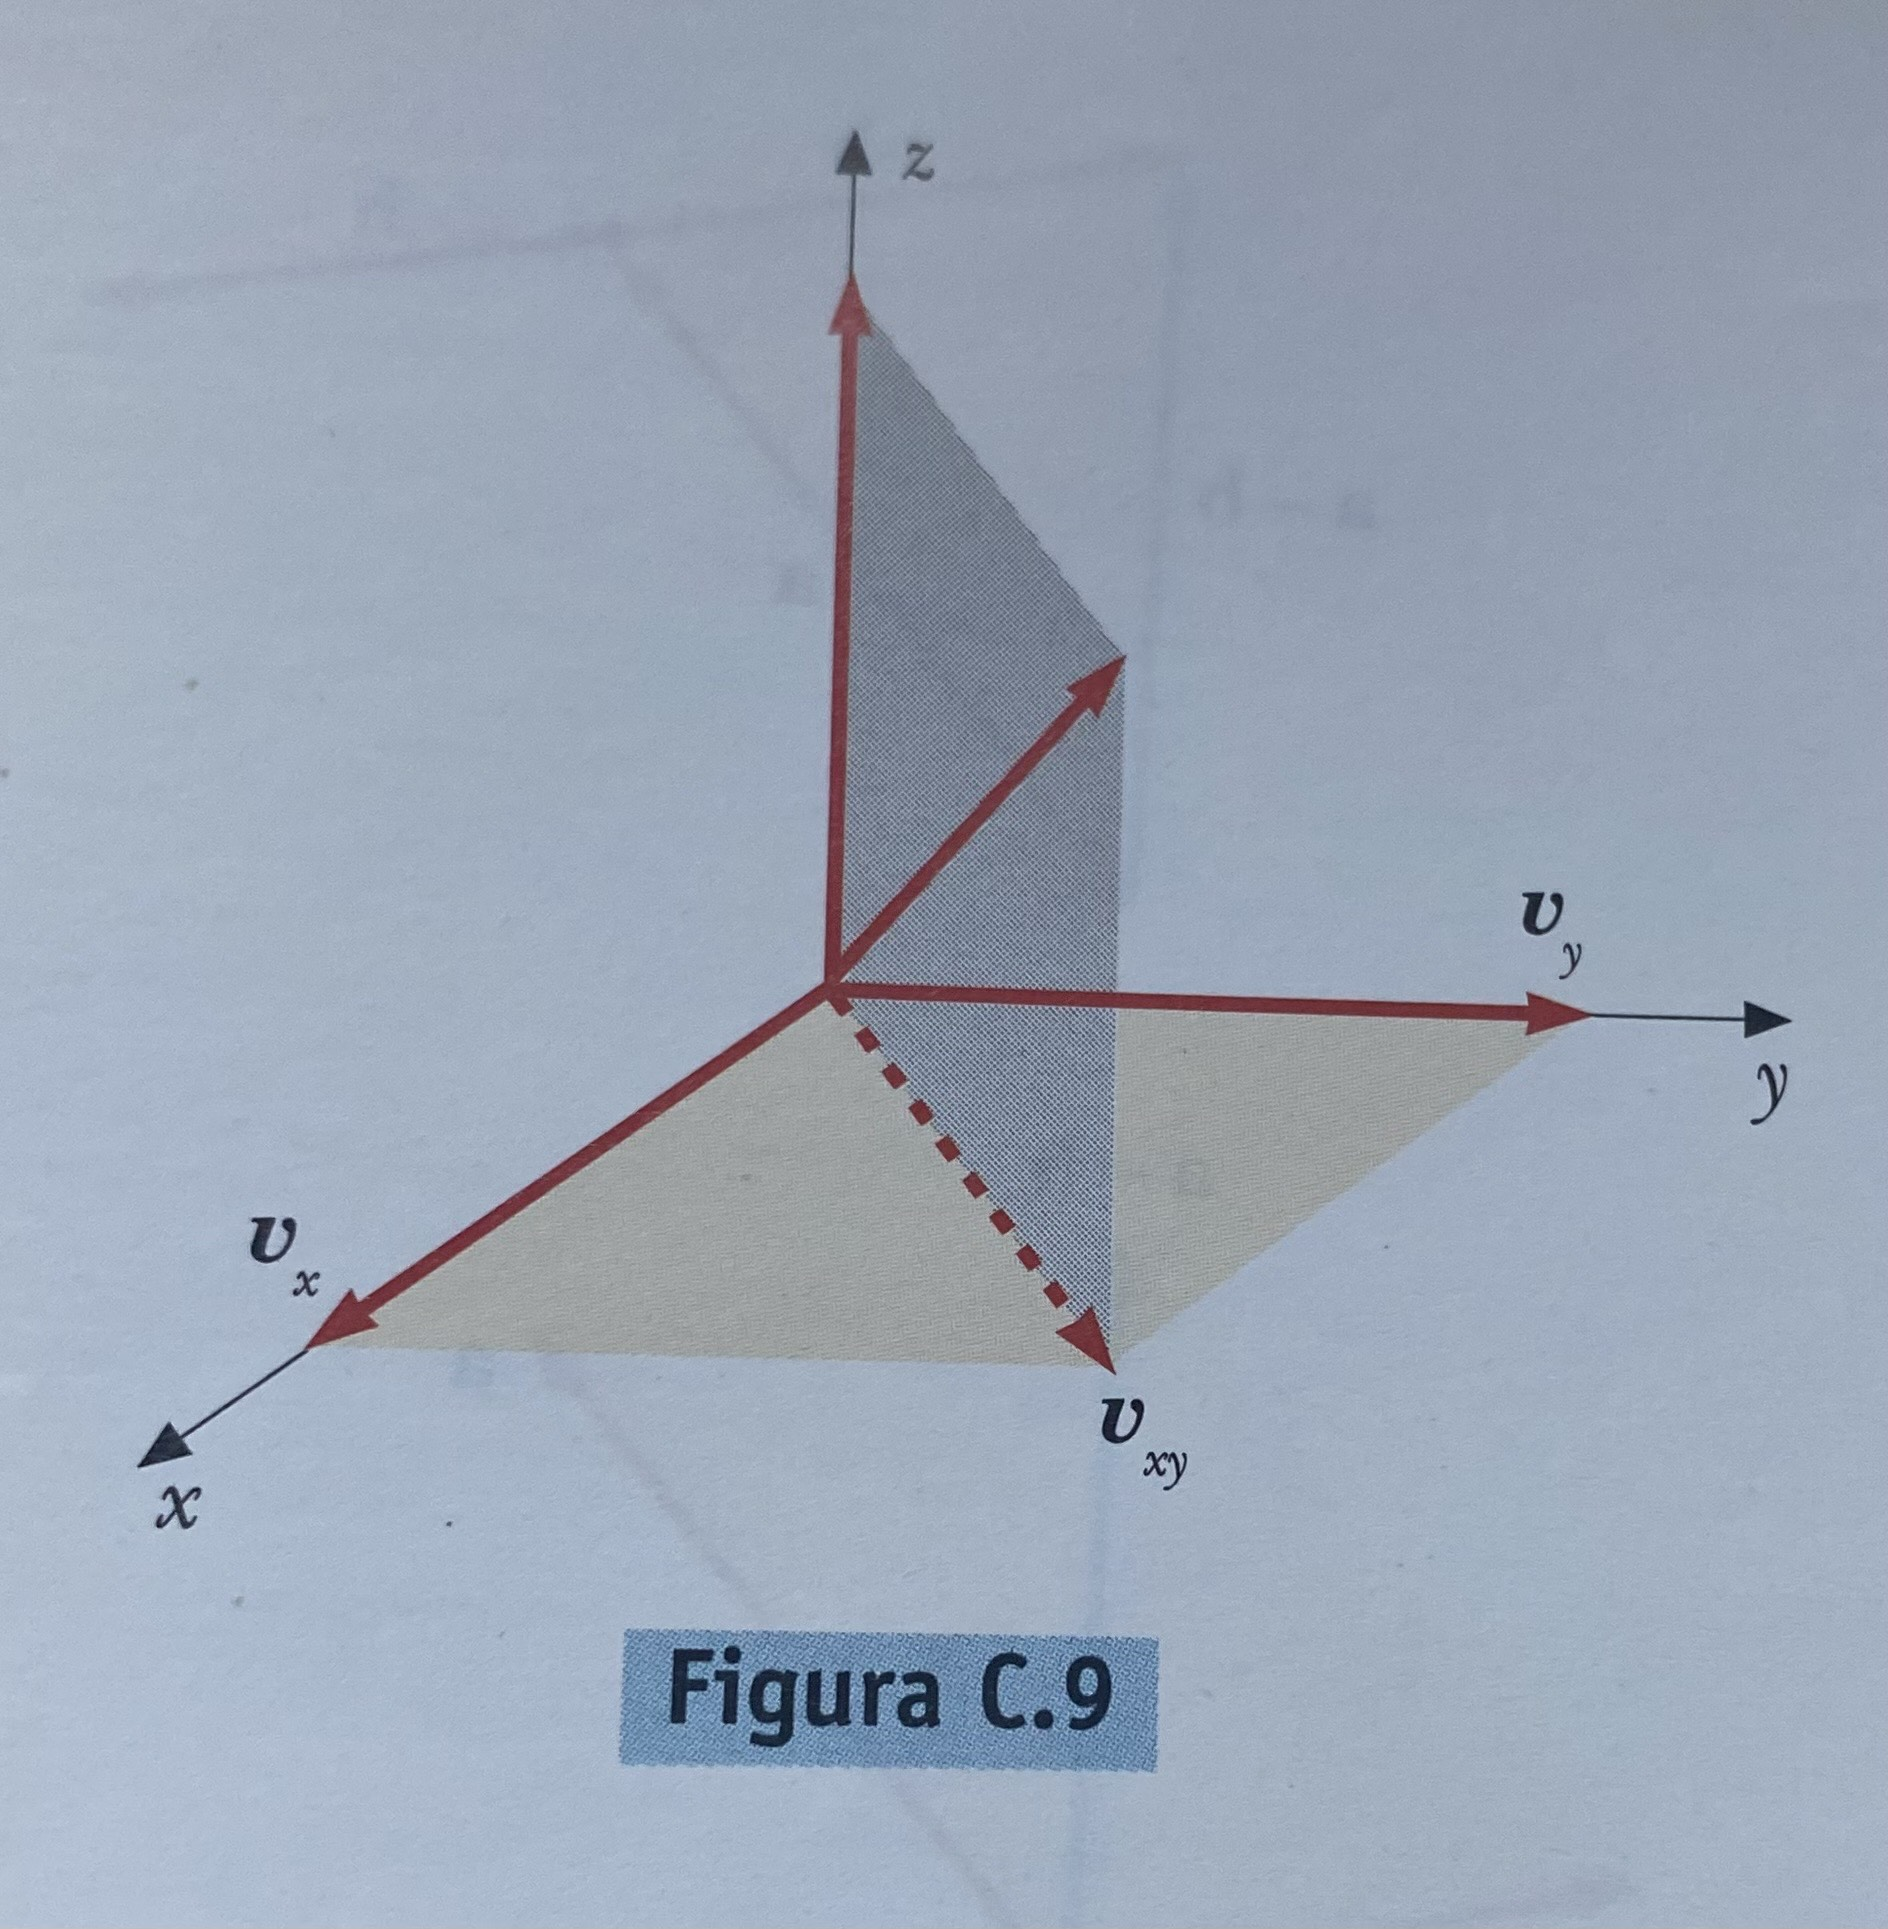
\includegraphics[width=4cm, height=4cm]{SComposizioneDiUnVettoreNelloSpazio.jpeg} % Percorso dell'immagine
    \caption{} % Didascalia per l'immagine
    \label{fig:immagine} % Etichetta per riferimento
\end{figure}
\noindent
I vettori $v_x,v_y,v_z$ si chiamano \textbf{vettori componenti} di $v$, mentre $u_x,u_y,u_z$ si chiamano \textbf{le componenti} di v secondo i tre assi cartesiani del sistema di riferimento prescelto. Quindi:
\begin{equation}
    a+b=(a_x+b_x)u_x + (a_y+b_y)u_y+(a_z+b_z)u_z
\end{equation}
\textbf{Il vettore somma ha come componenti la somma delle componenti dei singoli vettori.}
\subsubsection{Proprietà di invarianza}
Si pone il problema se il concetto di vettore e le operazioni che abbiamo finora definito, dipendano dal particolare sistema di riferimento prescelto. \textbf{Una grandezza scalare è invariante rispetto al sistema di riferimento}. Ne discende quindi che anche le operazioni di somma e prodotto per uno scalare sono \textbf{invarianti} rispetto alla scelta del sistema. Di conseguenza possiamo dire che quando le \textbf{equazioni} fisiche sono \textbf{scalari} oppure \textbf{vettoriali}, esse \textbf{hanno una validità intrinseca che non dipende dal sistema di riferimento}. Osserviamo inoltre, che quando scriviamo un'equazione vettoriale del tipo a=b e la consideriamo in un determinato sistema di riferimento. le tre equazioni $a_x=b_x, \ a_y=b_y, \ a_z=b_z$ sono valide come struttura in qualsiasi sistema, però con valori delle componenti diversi in ciascun sistema. Le \textbf{componenti} stesse, non essendo indipendenti dal sistema, \textbf{non sono quantità scalari}. Invece è uno scalare il modulo di un vettore:
\begin{equation}
    v=\sqrt{v_x^2+v_y^2+v_z^2}
\end{equation}
\newpage
\subsection{Prodotti tra vettori}
\subsubsection{Prodotto scalare}
Dati due vettori a e b si definisce \textbf{prodotto scalare}, la quantità:
\begin{equation}
    s=a \cdot b= a \ b\ cos\theta
\end{equation}
\begin{figure}[H] % Usa 'H' per forzare la posizione qui
    \centering % Centra l'immagine
    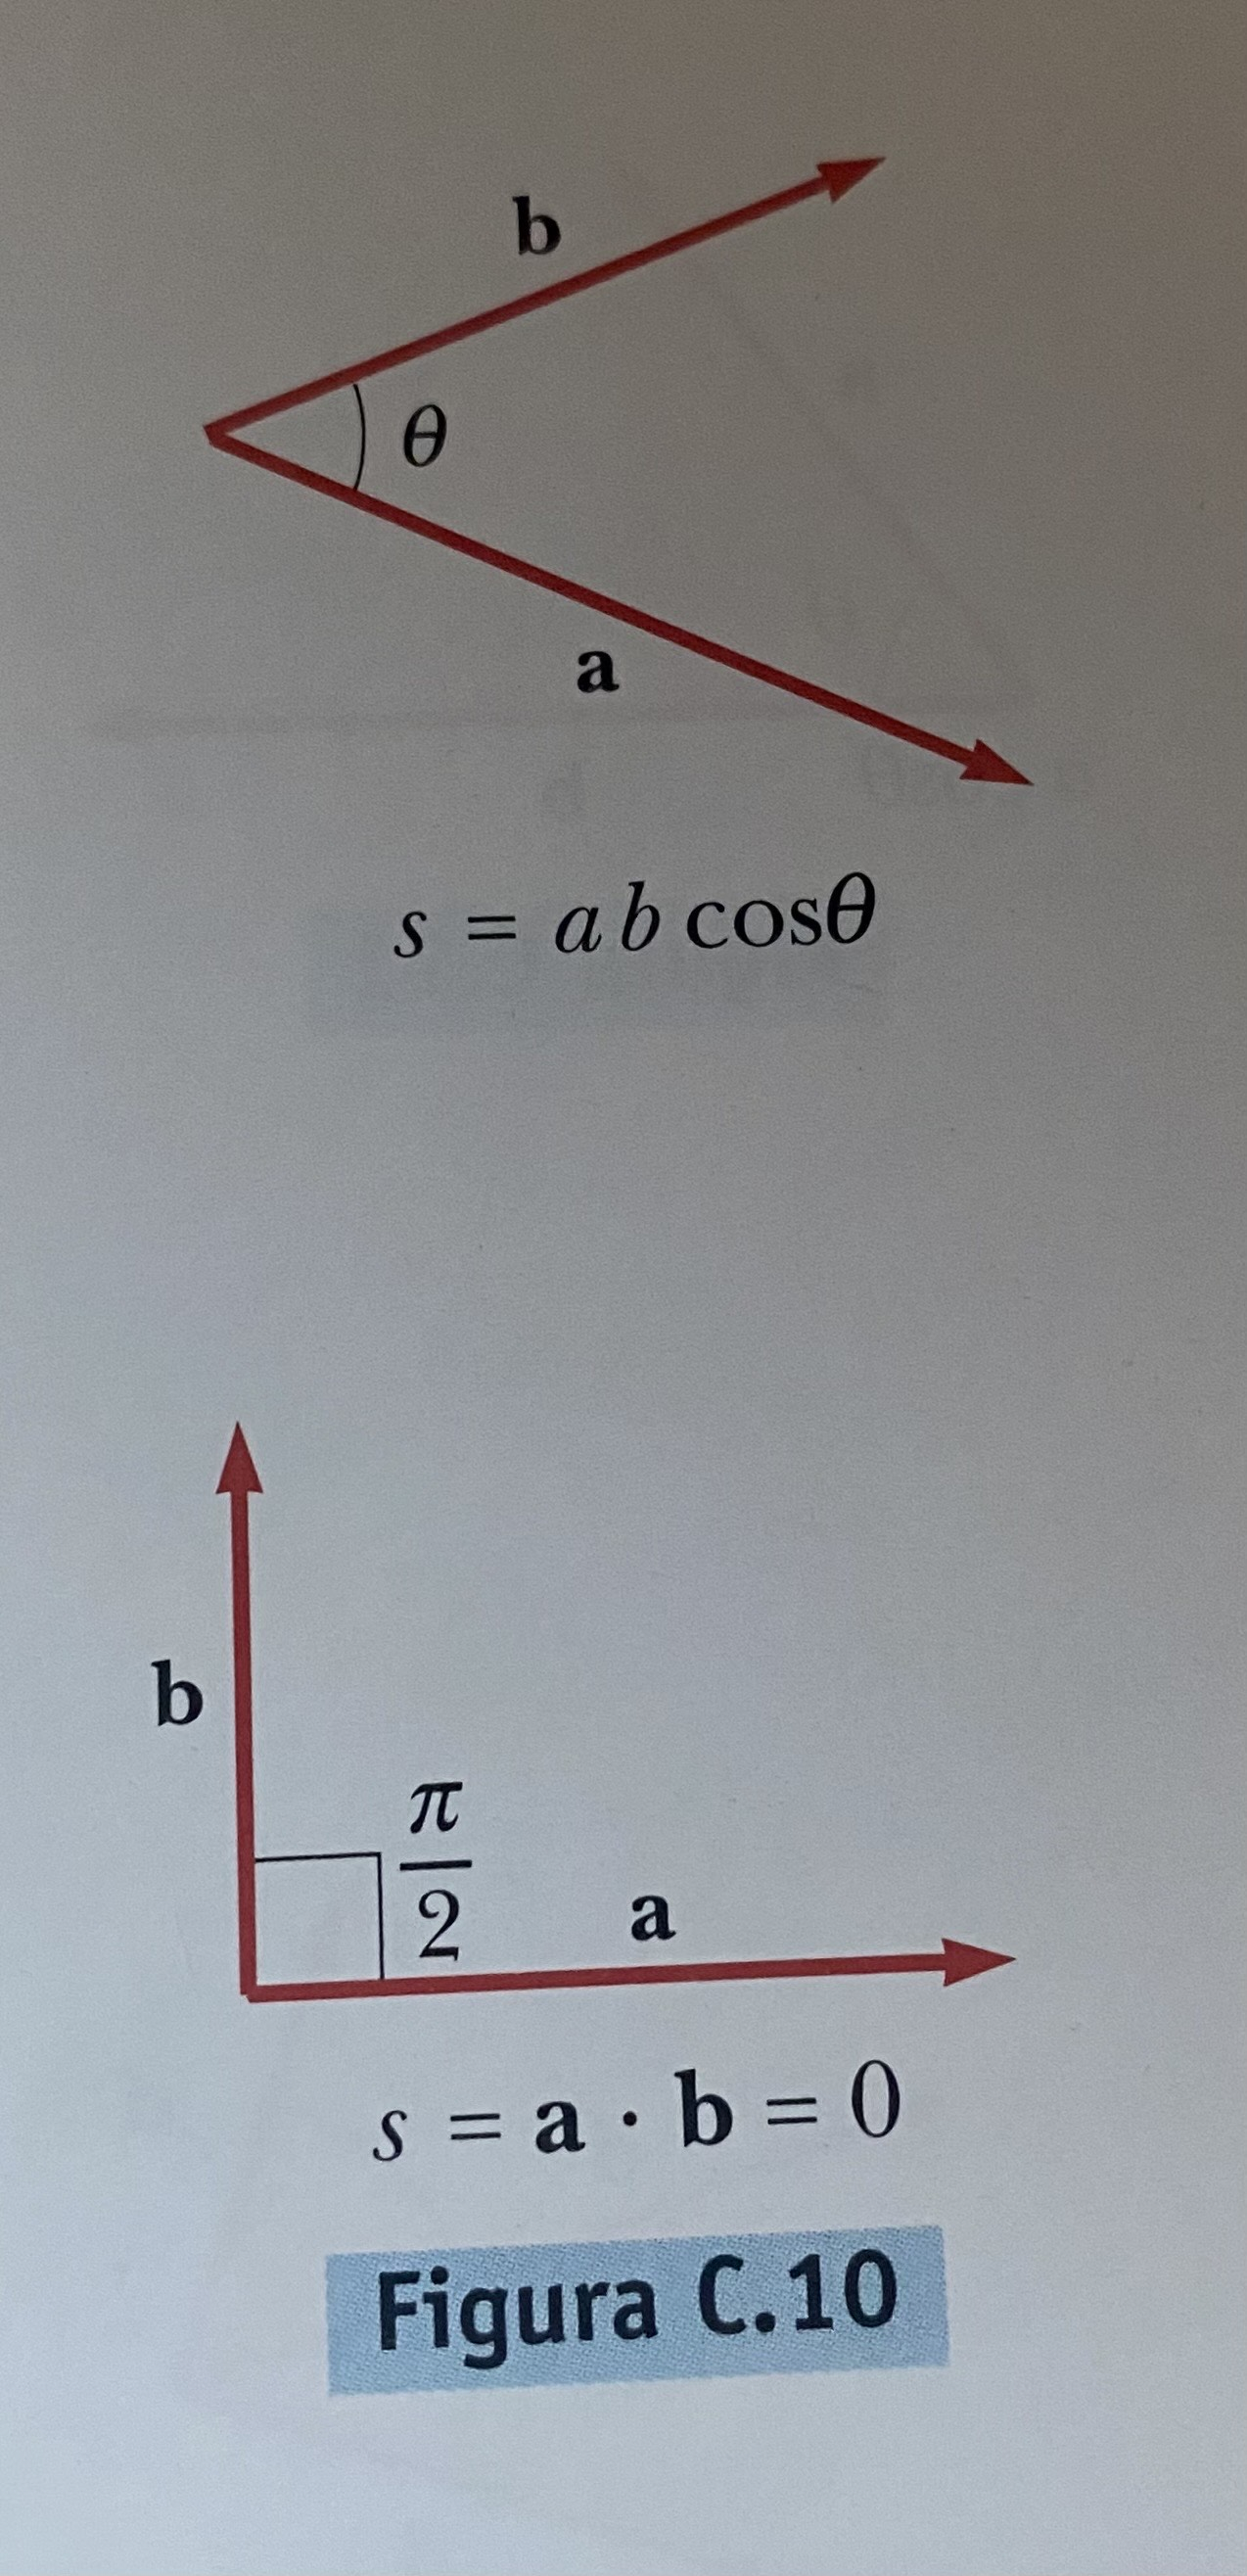
\includegraphics[width=4cm, height=6cm]{ProdottoScalare.jpeg} % Percorso dell'immagine
    \caption{} % Didascalia per l'immagine
    \label{fig:immagine} % Etichetta per riferimento
\end{figure}
\noindent
Indicando con $\theta$ l'angolo formato dai due vettori. Il risultato del prodotto scalare è una quantità scalare data dal prodotto dei moduli di a e b per il coseno dell'angolo compreso tra a e b. Il prodotto scalare gode delle seguenti proprietà:
\begin{itemize}
    \item è nullo non solo se uno dei due vettori è nullo, ma anche se i due vettori formano un angolo di $\pi/2$;
    \item vale la proprietà \textbf{commutativa};
    \item se $a=b$:
    \begin{equation}
        a \cdot a = |a|^2
    \end{equation}
    Il prodotto scalare di un vettore per se stesso, detto anche \textbf{quadrato del vettore}, \textbf{è eguale al quadrato del modulo del vettore.}
    \item non ha senso iterare il prodotto scalare: la scrittura $a \cdot b \cdot c$ è priva di significato perchè $a \cdot b$ è uno scalare e non può essere moltiplicato scalarmente per c.
    \item vale la \textbf{proprietà distributiva}
    \item se $c=a+b$, dalla proprietà distributiva e dal quadrato del vettore:
    \begin{equation}
    c^2=(a+b) \cdot (a+b) = a^2 + b^2 + 2 a\cdot b= a^2+b^2+2ab \ cos \theta
    \end{equation}
    che è il \textbf{teorema di Carnot} o del coseno per il triangolo avente come lati a, b, c e permette di calcolare subito il modulo della somma di due vettori. In particolare se $\theta=\pi /2$ si ritrova il \textbf{teorema di Pitagora} $c^2=a^2+b^2$
\end{itemize}
Il prodotto scalare tra due vettori \textbf{è eguale alla somma dei prodotti delle componenti omologhe dei singoli vettori}.
\begin{equation}
    a \cdot b = a_xb_x + a_yb_y + a_zb_z \ se \ a=b  \ -> a^2=a_x^2+a_y^2+a_z^2
\end{equation}
Il prodotto scalare tra due vettori \textbf{è eguale al prodotto del modulo di uno dei vettori per la proiezione su di questo dell'altro vettore.}
\begin{equation}
    s= a \cdot b = (a \ cos \theta)b= a (bcos\theta)
\end{equation}
\subsubsection{Prodotto Vettoriale}
\begin{figure}[H] % Usa 'H' per forzare la posizione qui
    \centering % Centra l'immagine
    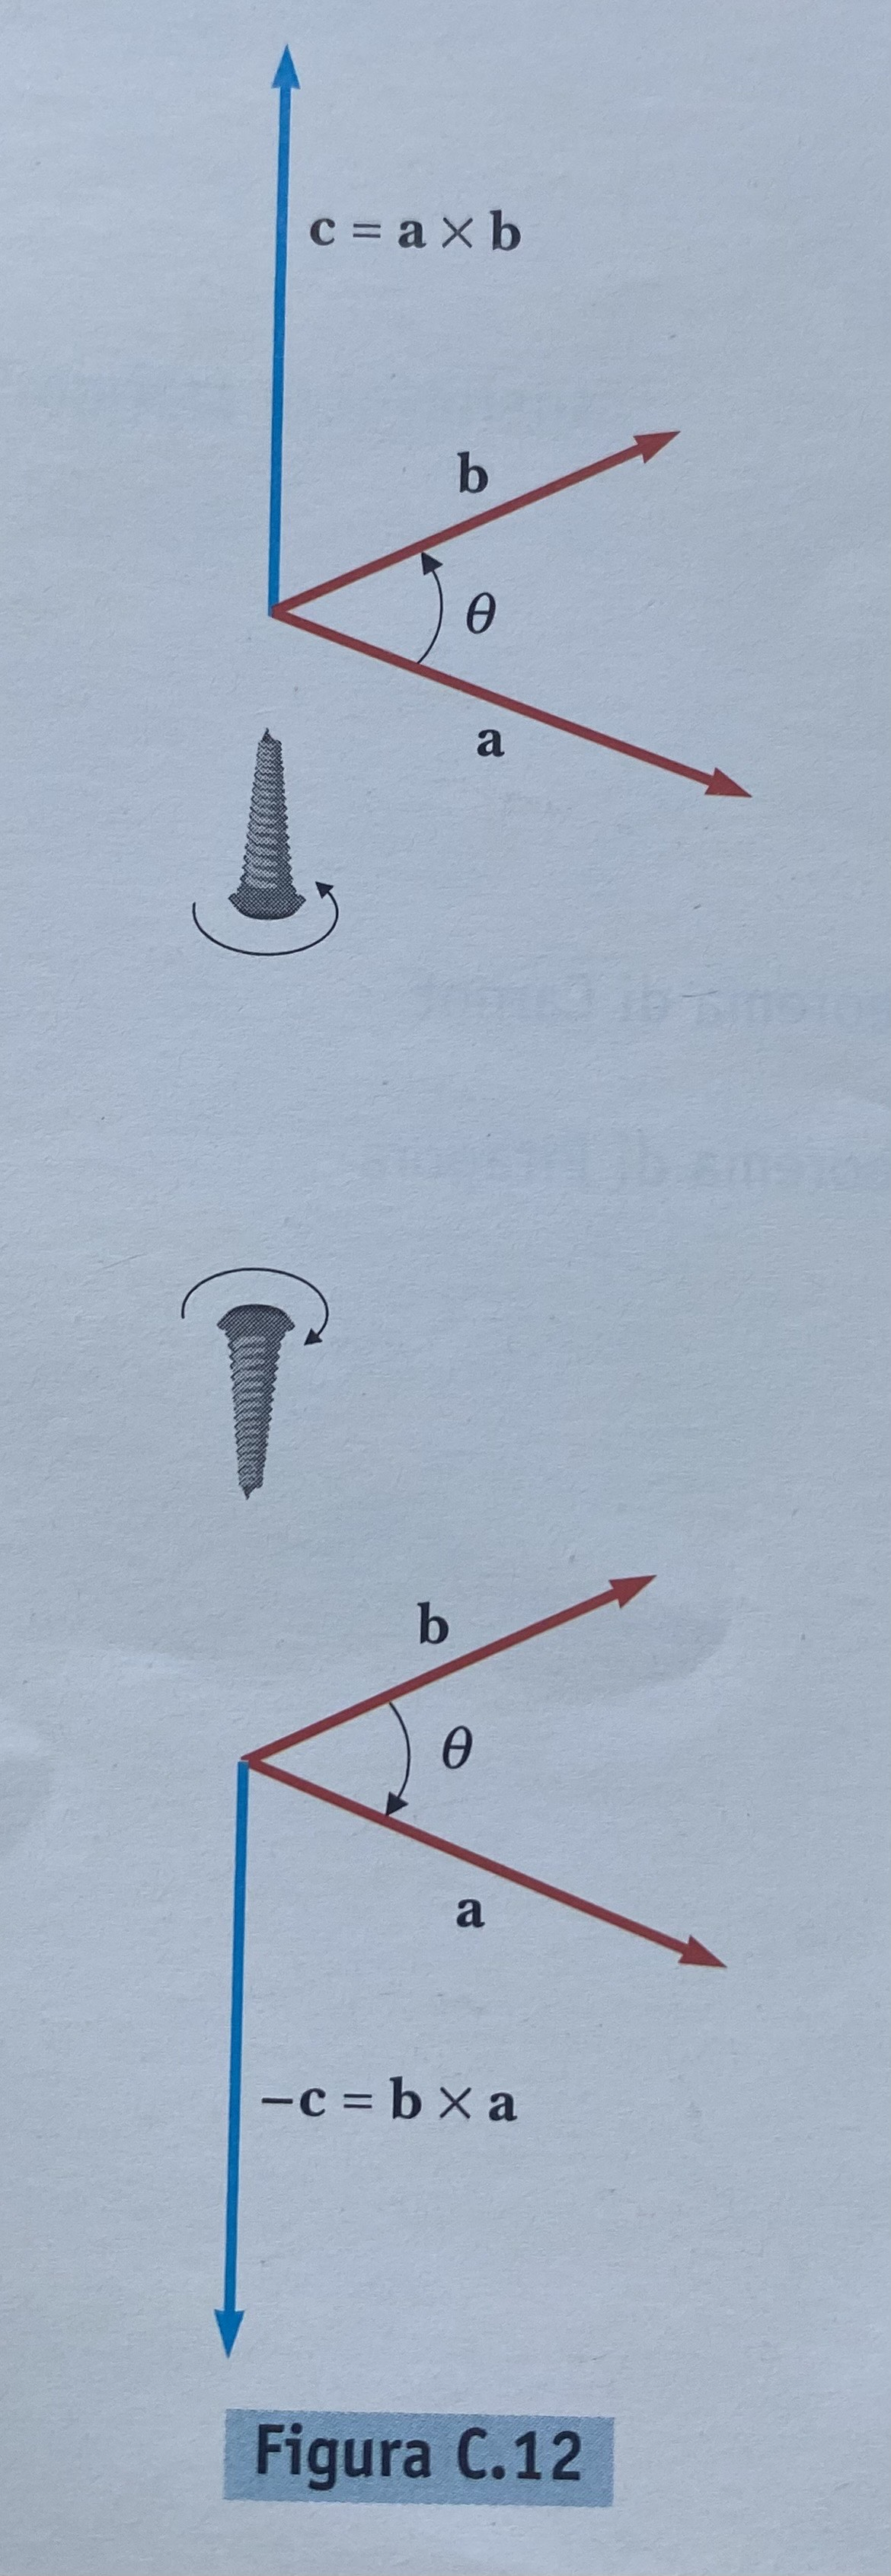
\includegraphics[width=4cm, height=7cm]{ProdottoVettoriale.jpeg} % Percorso dell'immagine
    \caption{} % Didascalia per l'immagine
    \label{fig:immagine} % Etichetta per riferimento
\end{figure}
\noindent
Dati due vettori a e b \textbf{prodotto vettoriale} il vettore c che si indica col simbolo:
\begin{equation}
    c = a \times b
\end{equation}
ed ha le seguenti caratteristiche:
\begin{itemize}
    \item la \textbf{direzione} è perpendicolare al piano individuato da a e b.
    \item il \textbf{verso} è quello di una normale vite destrogira, cioè ruotando da a a b nel verso della vite, il verso di c è indicato dalla punta della vite; alternativamente, si può dire che dalla punta di c deve apparire antioraria la rotazione che porta su a e b;
    \item il \textbf{modulo} è:
    \begin{equation}
        c= absen\theta
    \end{equation}
    e coincide con l'area del parallelogramma di lati a e b.
\end{itemize}
È bene osservare subito che il prodotto vettoriale non gode della \textbf{proprietà commutativa}. Difatti il \textbf{prodotto vettoriale è anticommutativo}. Valgono inoltre le seguenti proprietà:
\begin{itemize}
    \item Il risultato è nullo se uno dei due vettori è nullo oppure se i due vettori sono paralleli; in particolare è nullo il prodotto vettoriale di un vettore per se stesso.
    \item si applica la proprietà distributiva
    \item Il prodotto vettoriale può essere iterato, ma va completamente specificata la sequenza delle diverse operazioni, perchè \textbf{non vale la proprietà associativa:}
    \begin{equation}
        a \times (b \times c) \neq (a \times b) \times c
    \end{equation}
\end{itemize}
Il prodotto vettoriale è invariante.
\begin{equation}
    c = a \times b = (a_yb_z - a_zb_y)u_x + (a_zb_x - a_xb_z)u_y+(a_xb_y-a_yb_x)u_z
\end{equation}
che si può anche scrivere:
$
\begin{bmatrix}
u_x & u_y & u_z \\
a_x & a_y & a_z \\
b_x & b_y & b_z
\end{bmatrix}$
Il vettore c si calcola come \textbf{determinante} della matrice formata con i versori degli assi del sistema di riferimento, le componenti di a e quelle di b, nell'ordine prefissato. Un'altra rappresentazione molto utile consiste nello scomporre b secondo un componente $b_T$ parallelo ad a e un componente $b_N$ ortogonale ad a per cui:
\newpage
% Soluzione 1: Usa \raisebox per abbassare l'immagine
\noindent
\begin{minipage}[t]{0.4\textwidth}
  \raisebox{-\height}{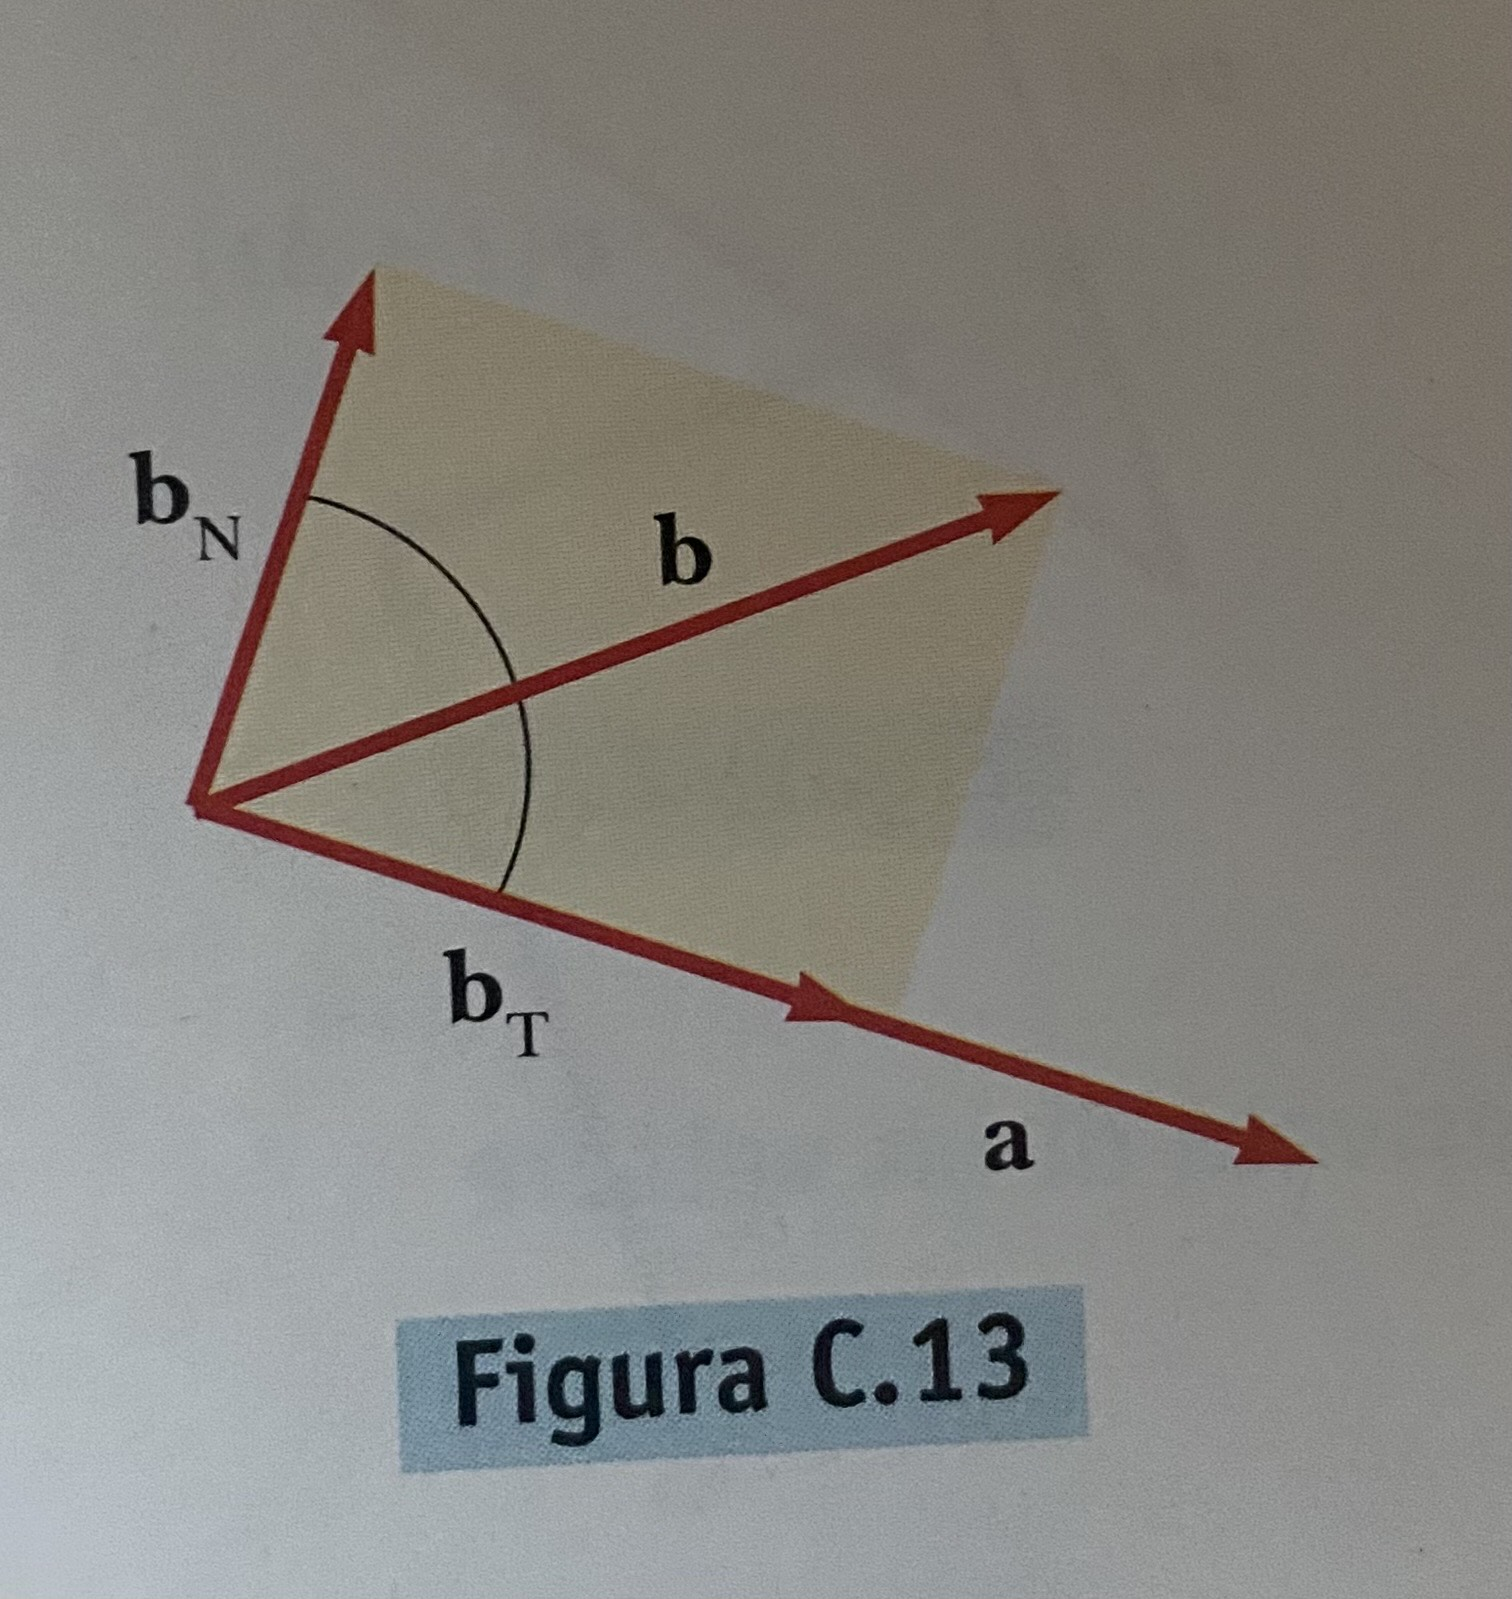
\includegraphics[width=\linewidth]{AltraRapProdottoScalare.jpeg}}
\end{minipage}%
\hfill
\begin{minipage}[t]{0.55\textwidth}
  \raggedright
  \[
  c= a \times b = a \times (b_T + b_N)= a \times b_N
  \]
  In quanto $a \times b_T=0$ essendo i due vettori paralleli. \textbf{Il modulo del prodotto vettoriale è eguale al prodotto del modulo di un vettore per la componente dell'altro vettore normale al primo.}
\end{minipage}
\subsubsection{Momento di un vettore}
Sia v un vettore applicato nel punto P e O un altro generico punto. Si definisce \textbf{momento del vettore v rispetto al punto o}, chiamato \textbf{polo}, il vettore:
\begin{equation}
    M_0 = OP \times v
\end{equation}
\noindent
\begin{minipage}[t]{0.4\textwidth}
  \raisebox{-\height}{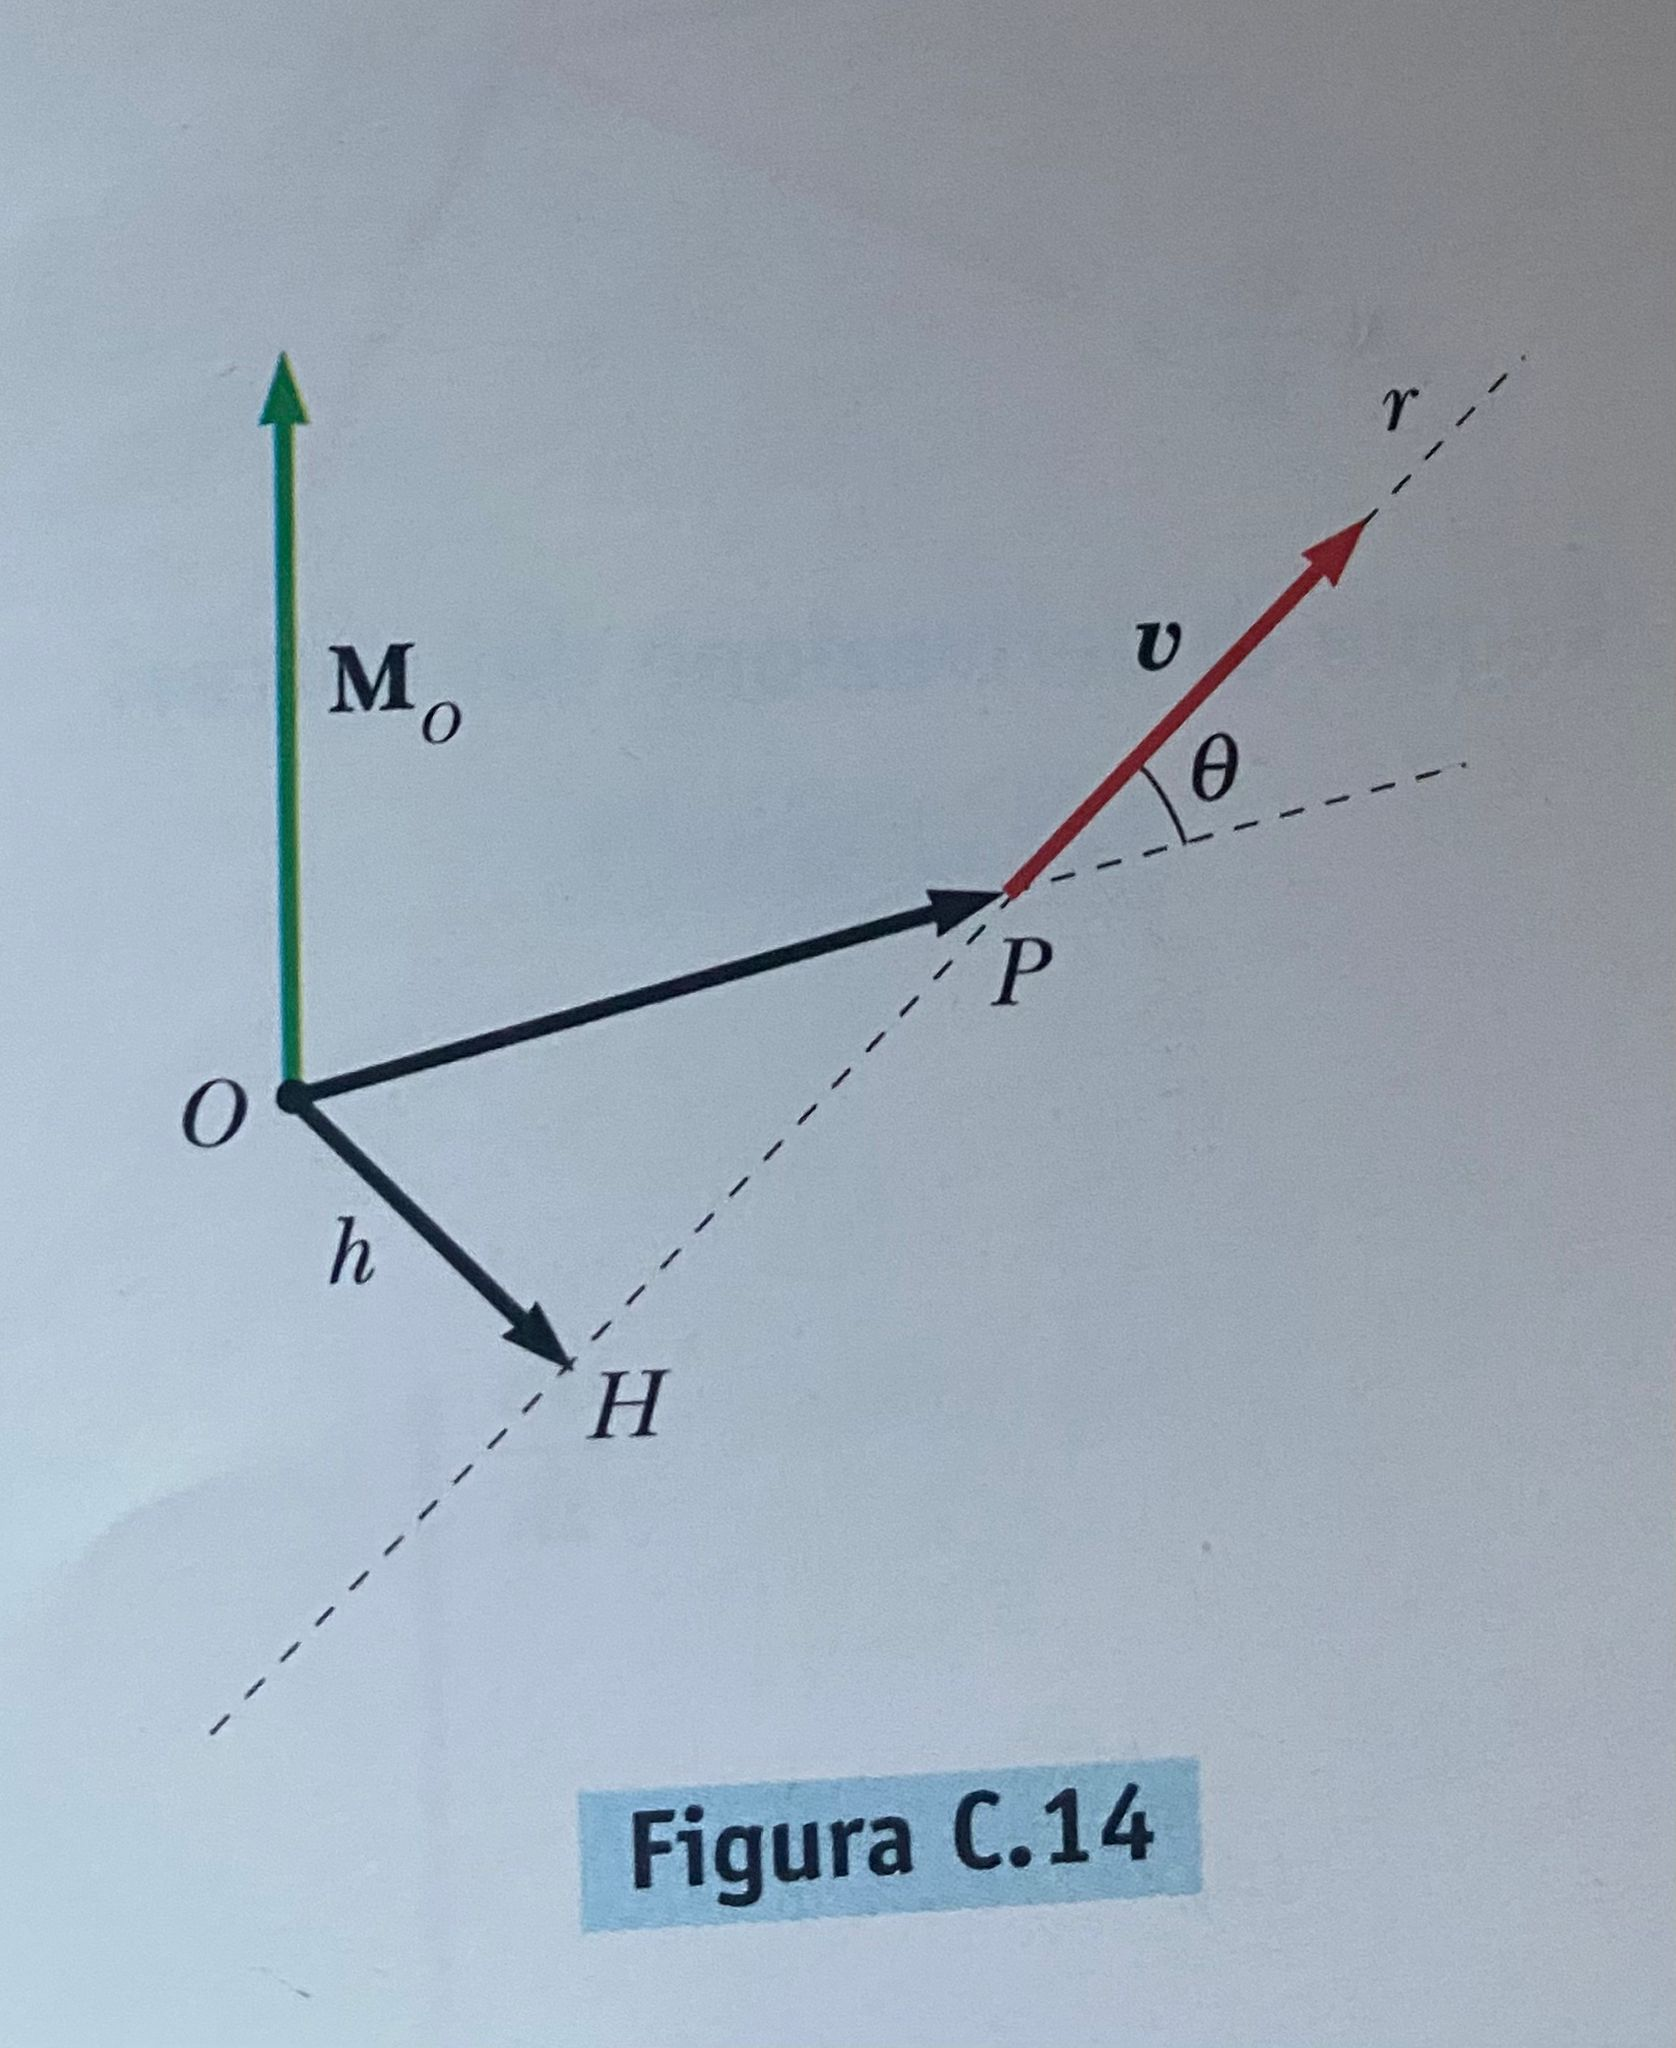
\includegraphics[width=\linewidth]{MomentoDiUnVettore.jpeg}}
\end{minipage}%
\hfill
\begin{minipage}[t]{0.55\textwidth}
  \raggedright
  ortogonale al piano individuato da OP e v. Detto OH il componente di OP perpendicolare a v, otteniamo:
  \begin{equation}
      M_0 = OP \times v=OH \times v
  \end{equation}
  Il modulo di $M_0$ è dato da:
  \begin{equation}
      M_0= |OP| v sen \theta = |OH| v=hv
  \end{equation}
  essendo h la distanza di O dalla retta r contenente v, detta \textbf{retta di applicazione} di v; h prende il nome di \textbf{braccio} di v rispetto a O. In generale: \textbf{il momento di un vettore dipende dal polo}, se si cambia polo cambia anche il momento.
  \end{minipage}
  \subsection{Derivata di un vettore}
  Consideriamo un vettore v funzione di una variabile scalare t, cioè una grandezza vettoriale il cui modulo e la cui direzione cambiano al variare di t, in un modo che in generale supponiamo continuo. v(t) e v(t+ $\Delta t$) sono due diversi valori della funzione, comprendendo nel termine valore modulo e direzione. Possiamo scrivere:
  \begin{equation}
      v(t+ \Delta t) = v(t) + \Delta v
  \end{equation}
  e costruire il rapporto
  \begin{equation}
      \frac{\Delta v
      }{\Delta t} = \frac{v(t + \Delta t)- v(t)}{\Delta t}
  \end{equation}
  Si definisce \textbf{derivata del vettore v rispetto alla variabile t} la quantità:
  \begin{equation}
      \frac{dv}{dt}= \frac{lim}{\Delta t -> 0}\frac{\Delta v}{\Delta t}=\frac{lim}{\Delta t -> 0} \frac{v(t+ \Delta t) - v(t)}{\Delta t}
  \end{equation}
  La derivata di un vettore è ancora un vettore. Inoltre il valore derivata in generale non è parallelo a v. Per la derivata valgono le usuali \textbf{regole di derivazione}, come ad esempio:
  \begin{align}
      & \frac{d}{dt}(a + b) = \frac{da}{dt}+\frac{db}{dt} \\
      & \frac{d}{dt}(m\vec{v}) = m\frac{dv}{dt} \ se \ m \ \text{è} \ costante\\
      &\frac{d}{dt}(m\vec{v}) = \frac{dm}{dt}v+m\frac{dv}{dt} \ se \ m \ dipende \ da \ t \\
      & \frac{d}{dt}(a \cdot b) = \frac{da}{dt} \cdot b + a \cdot \frac{db}{dt} \\
      & \frac{d}{dt}(a \times b) = \frac{da}{dt} \times b + a \times \frac{db}{dt} 
  \end{align}
La derivata di un vettore è \textbf{invariante}. Se però rappresentiamo il vettore v in un sistema di assi cartesiani ortogonali per cui $v=v_xu_x+v_yu_y+v_zu_z$, allora ripetendo il procedimento di passaggio al limite abbiamo: \textbf{derivata di un vettore}:
\begin{equation}
    \frac{dv}{dt}=\frac{dv_x}{dt}u_x + \frac{dv_y}{dt}u_y + \frac{dv_z}{dt}u_z
\end{equation}
\subsubsection{Derivata di un versore u(t)}
Dal momento che un versore è per definizione un vettore di modulo unitario, ciò che può cambiare in funzione di t è solo la direzione, cioè il versore può compiere solamente una rotazione di un certo angolo $\Delta \theta$. 
\newpage
\noindent
\begin{minipage}[t]{0.4\textwidth}
  \raisebox{-\height}{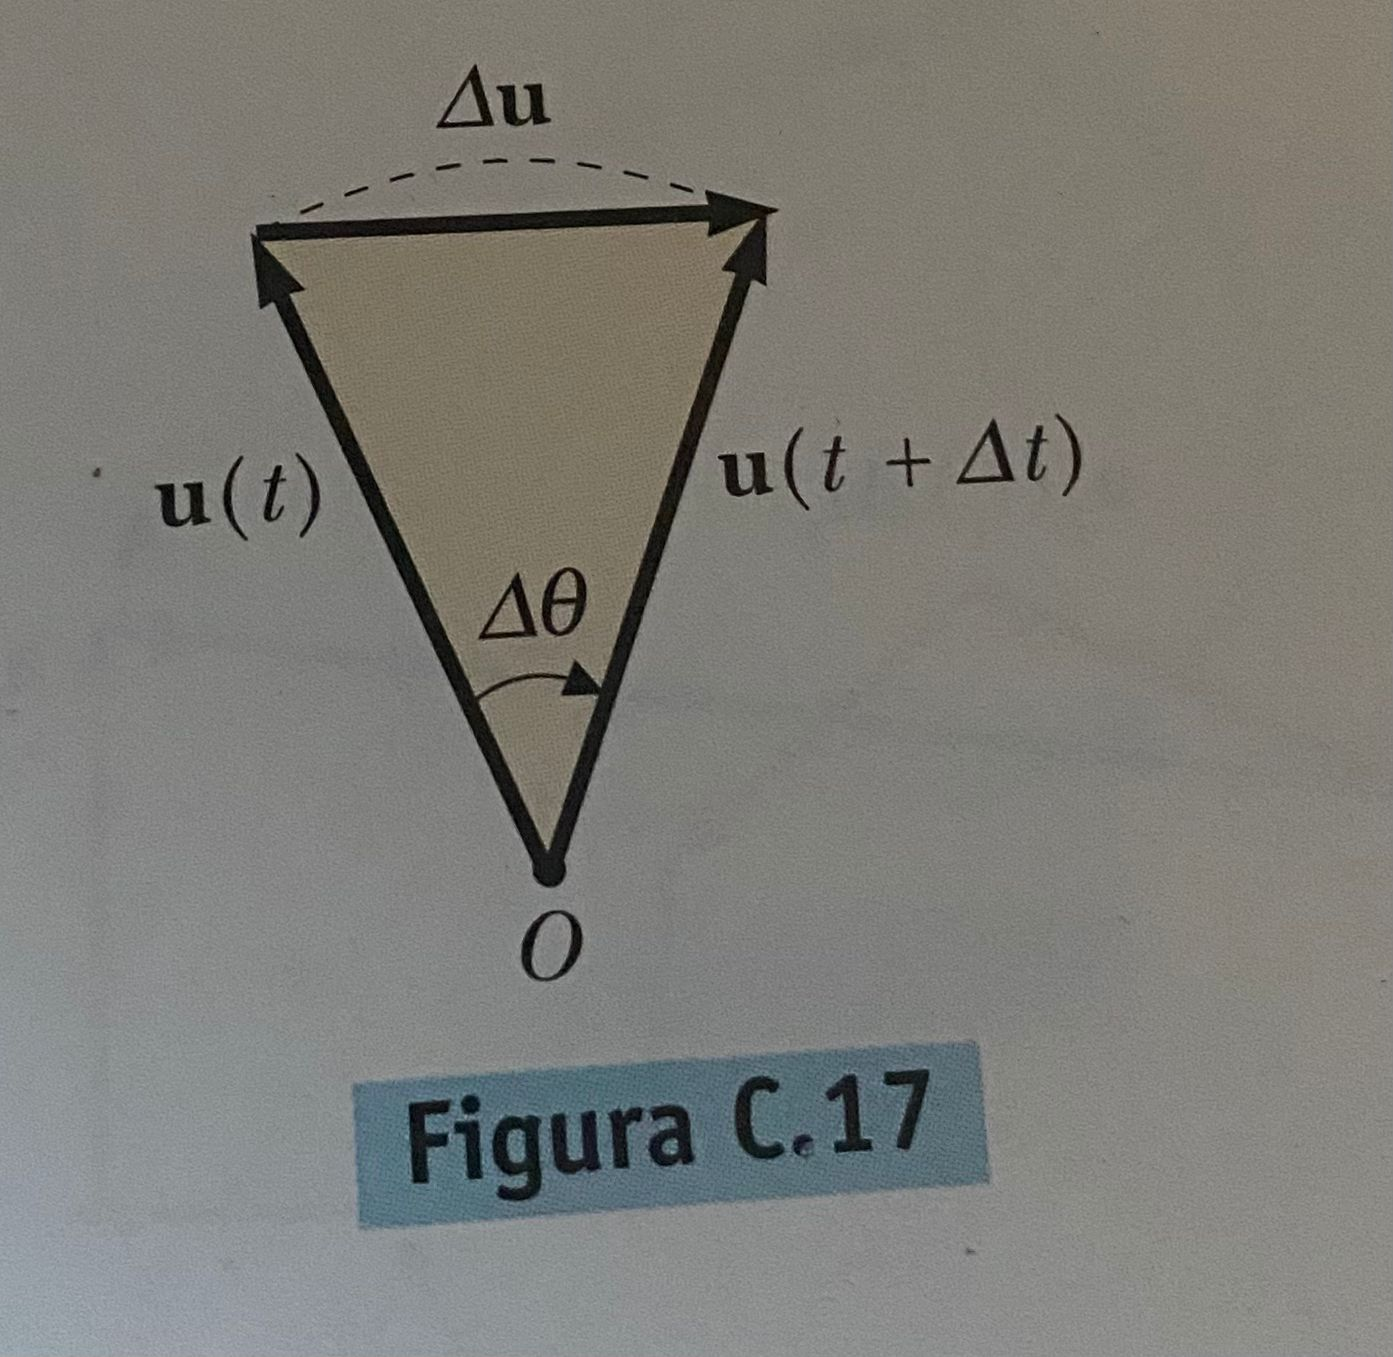
\includegraphics[width=\linewidth]{DerivataDiUnVersore.jpeg}}
\end{minipage}%
\hfill
\begin{minipage}[t]{0.55\textwidth}
  \raggedright
  Possiamo quindi scrivere
  \begin{equation}
      \Delta u = u(t + \Delta t) - u(t)
  \end{equation}
 essendo $\Delta u$ la corda che unisce gli estremi dell'arco di circonferenza descritto da u(t) nella rotazione di $\Delta \theta$. Al limite per $\Delta t -> 0$ la corda $\Delta u$ tende ad un vettore infinitesimo du, \textbf{perpendicolare} a u(t), il cui modulo si confonde con l'arco:
 \begin{equation}
     du = |u(t)|d \theta= d\theta \ -> \ du=d \theta u_N
 \end{equation}
 essendo $u_N$ \textbf{un versore perpendicolare a u(t)}.
  \end{minipage}

\begin{minipage}[t]{0.4\textwidth}
  \raisebox{-\height}{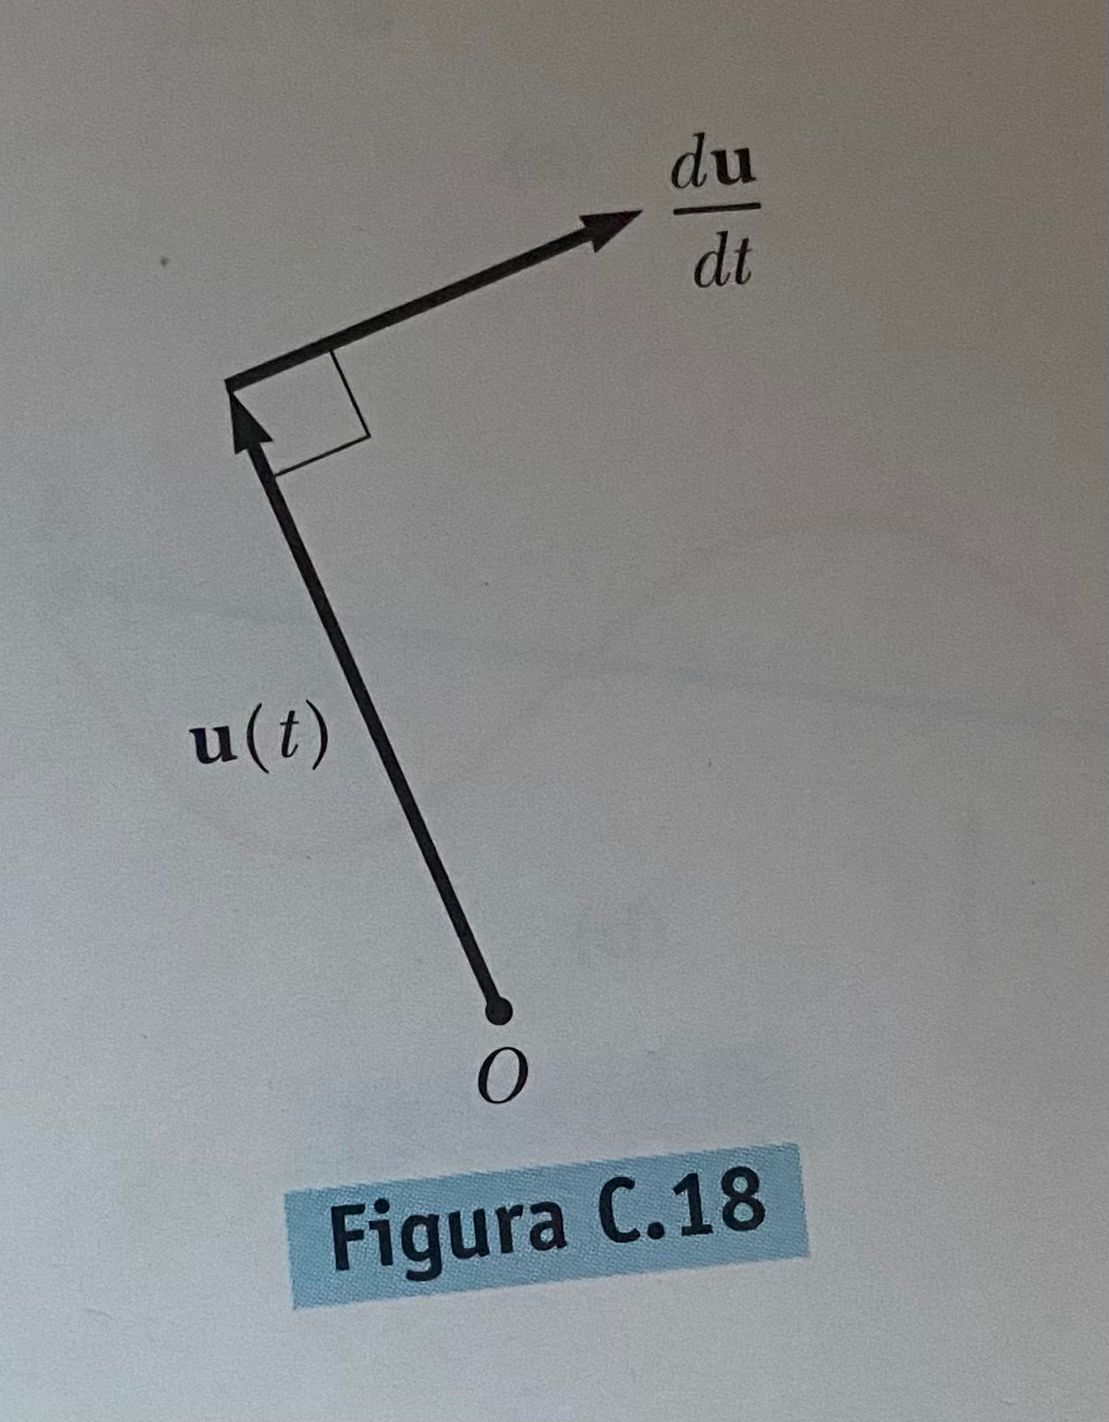
\includegraphics[width=\linewidth]{DerivataDiUnVersore2.jpeg}}
\end{minipage}%
\hfill
\begin{minipage}[t]{0.55\textwidth}
  \raggedright
  Definiamo la \textbf{derivata di un versore u(t)} come:
  \begin{equation}
      \frac{du}{dt}= \frac{d \theta}{dt}u_N
  \end{equation}
\textbf{La derivata di un versore è un vettore perpendicolare al versore, di modulo $d \theta/dt$, in generale diverso da 1: in altre parole du/dt non è un versore}.
  \end{minipage}
  \subsubsection{Scrittura intrinseca della derivata}
  Il \textbf{modulo del vettore derivato è}
  \begin{equation}
      |\frac{dv}{dt}|= \sqrt{(\frac{dv}{dt})^2+(v\frac{d \theta}{dt})^2}
  \end{equation}
  osservando che il modulo della derivata di v è diverso dalla derivata del modulo di v. \textbf{La derivata di un vettore di modulo costante è perpendicolare al vettore stesso.}
  \subsection{Integrazione Vettoriale}
  Si definisce \textbf{integrale definito} di a(t):
  \begin{equation}
      A = \int_{t_1}^{t_2} a(t) dt
  \end{equation}
  Il vettore A(t) ottenuto dall'integrazione non dipende dal sistema di riferimento. Tuttavia per eseguire i calcoli è conveniente fissare un sistema di coordinate, per esempio cartesiane ortogonali e l'integrale si scrive:
  \begin{equation}
      A = \int_{t_1}^{t_2} a(t) = u_x \int_{t_1}^{t_2} a_x(t) + u_y \int_{t_1}^{t_2} a_y(t) + u_z \int_{t_1}^{t_2} a_z(t) 
  \end{equation}
  \textbf{l'integrale di un vettore ha come componenti gli integrali delle componenti del vettore}.
  \subsubsection{Integrale di linea}
  \begin{minipage}[t]{0.4\textwidth}
  \raisebox{-\height}{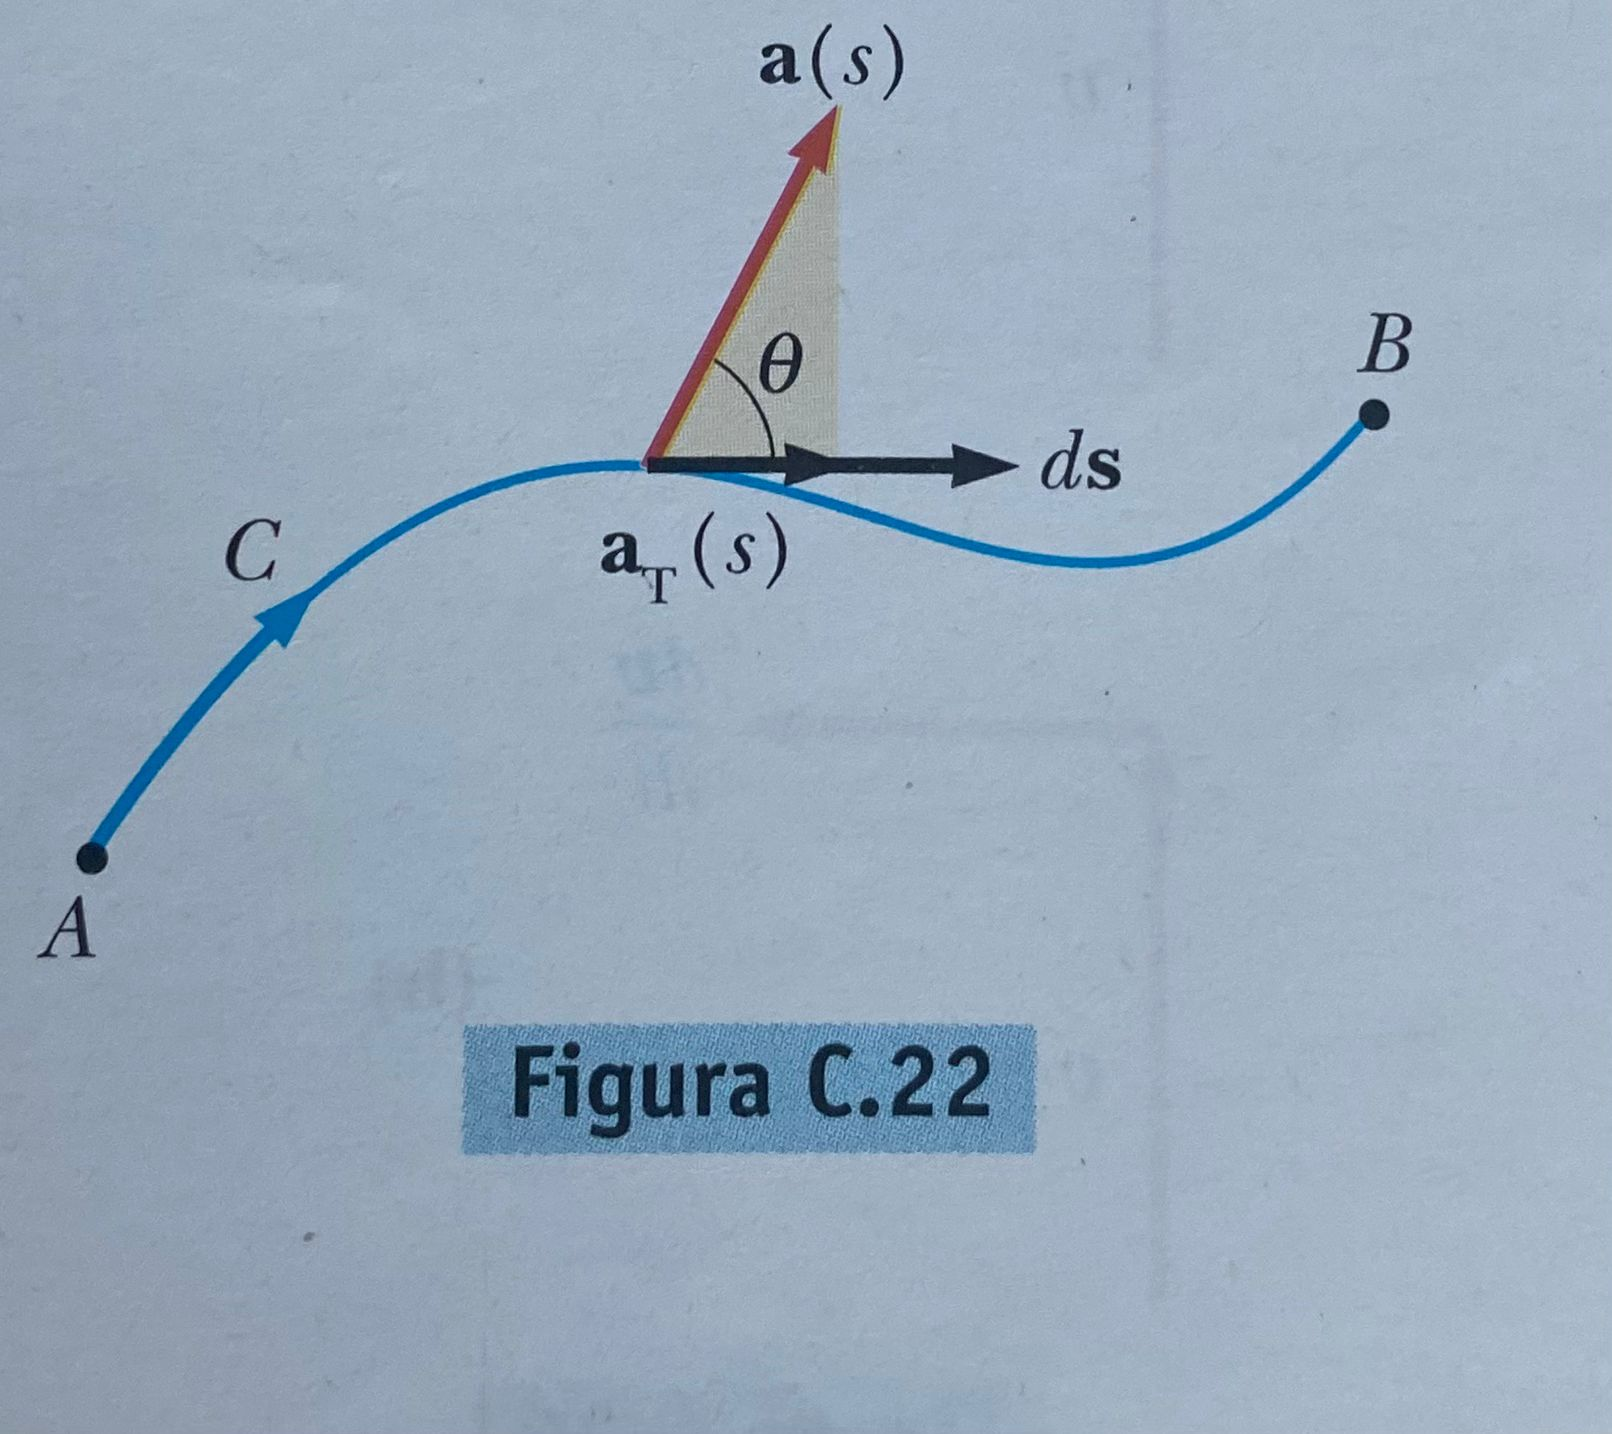
\includegraphics[width=\linewidth]{IntegraleDiLinea.jpeg}}
\end{minipage}%
\hfill
\begin{minipage}[t]{0.55\textwidth}
  \raggedright
  Consideriamo una curva continua C, di estremi A e B, nei punti della quale è definito un vettore a(s), essendo s una coordinata curvilinea che individua il punto corrente sulla curva. Se ds è un vettore infinitesimo tangente alla curva nel punto P, calcoliamo il prodotto scalare:
  \begin{equation}
      a(s) \cdot ds = a(s) cos \theta ds =a_T(s)ds
  \end{equation}
  dove $a_T(s)$ è la componente di a(s) tangente alla curva nel piano P. Si sommano tutti questi infiniti contributi infinitesimi ottenuti suddividendo la curva C in infiniti elementi ds; il risultato si chiama \textbf{integrale di linea} di a lungo la curva C orientata da A a B e si indica con:
  \begin{equation}
      \mathcal{T}(A->B \ lungo \ C) = \int_A^B a \cdot ds
  \end{equation}
  \textbf{L'integrale di linea è uno scalare.} Se la curva è chiusa ($A=B$) si parla di \textbf{circuitazione di a lungo la linea chiusa}, e si usa il simbolo:
  \begin{equation}
      \oint a \cdot ds
  \end{equation}
  \end{minipage}
\subsubsection{Integrale di superficie}
  \begin{minipage}[t]{0.4\textwidth}
  \raisebox{-\height}{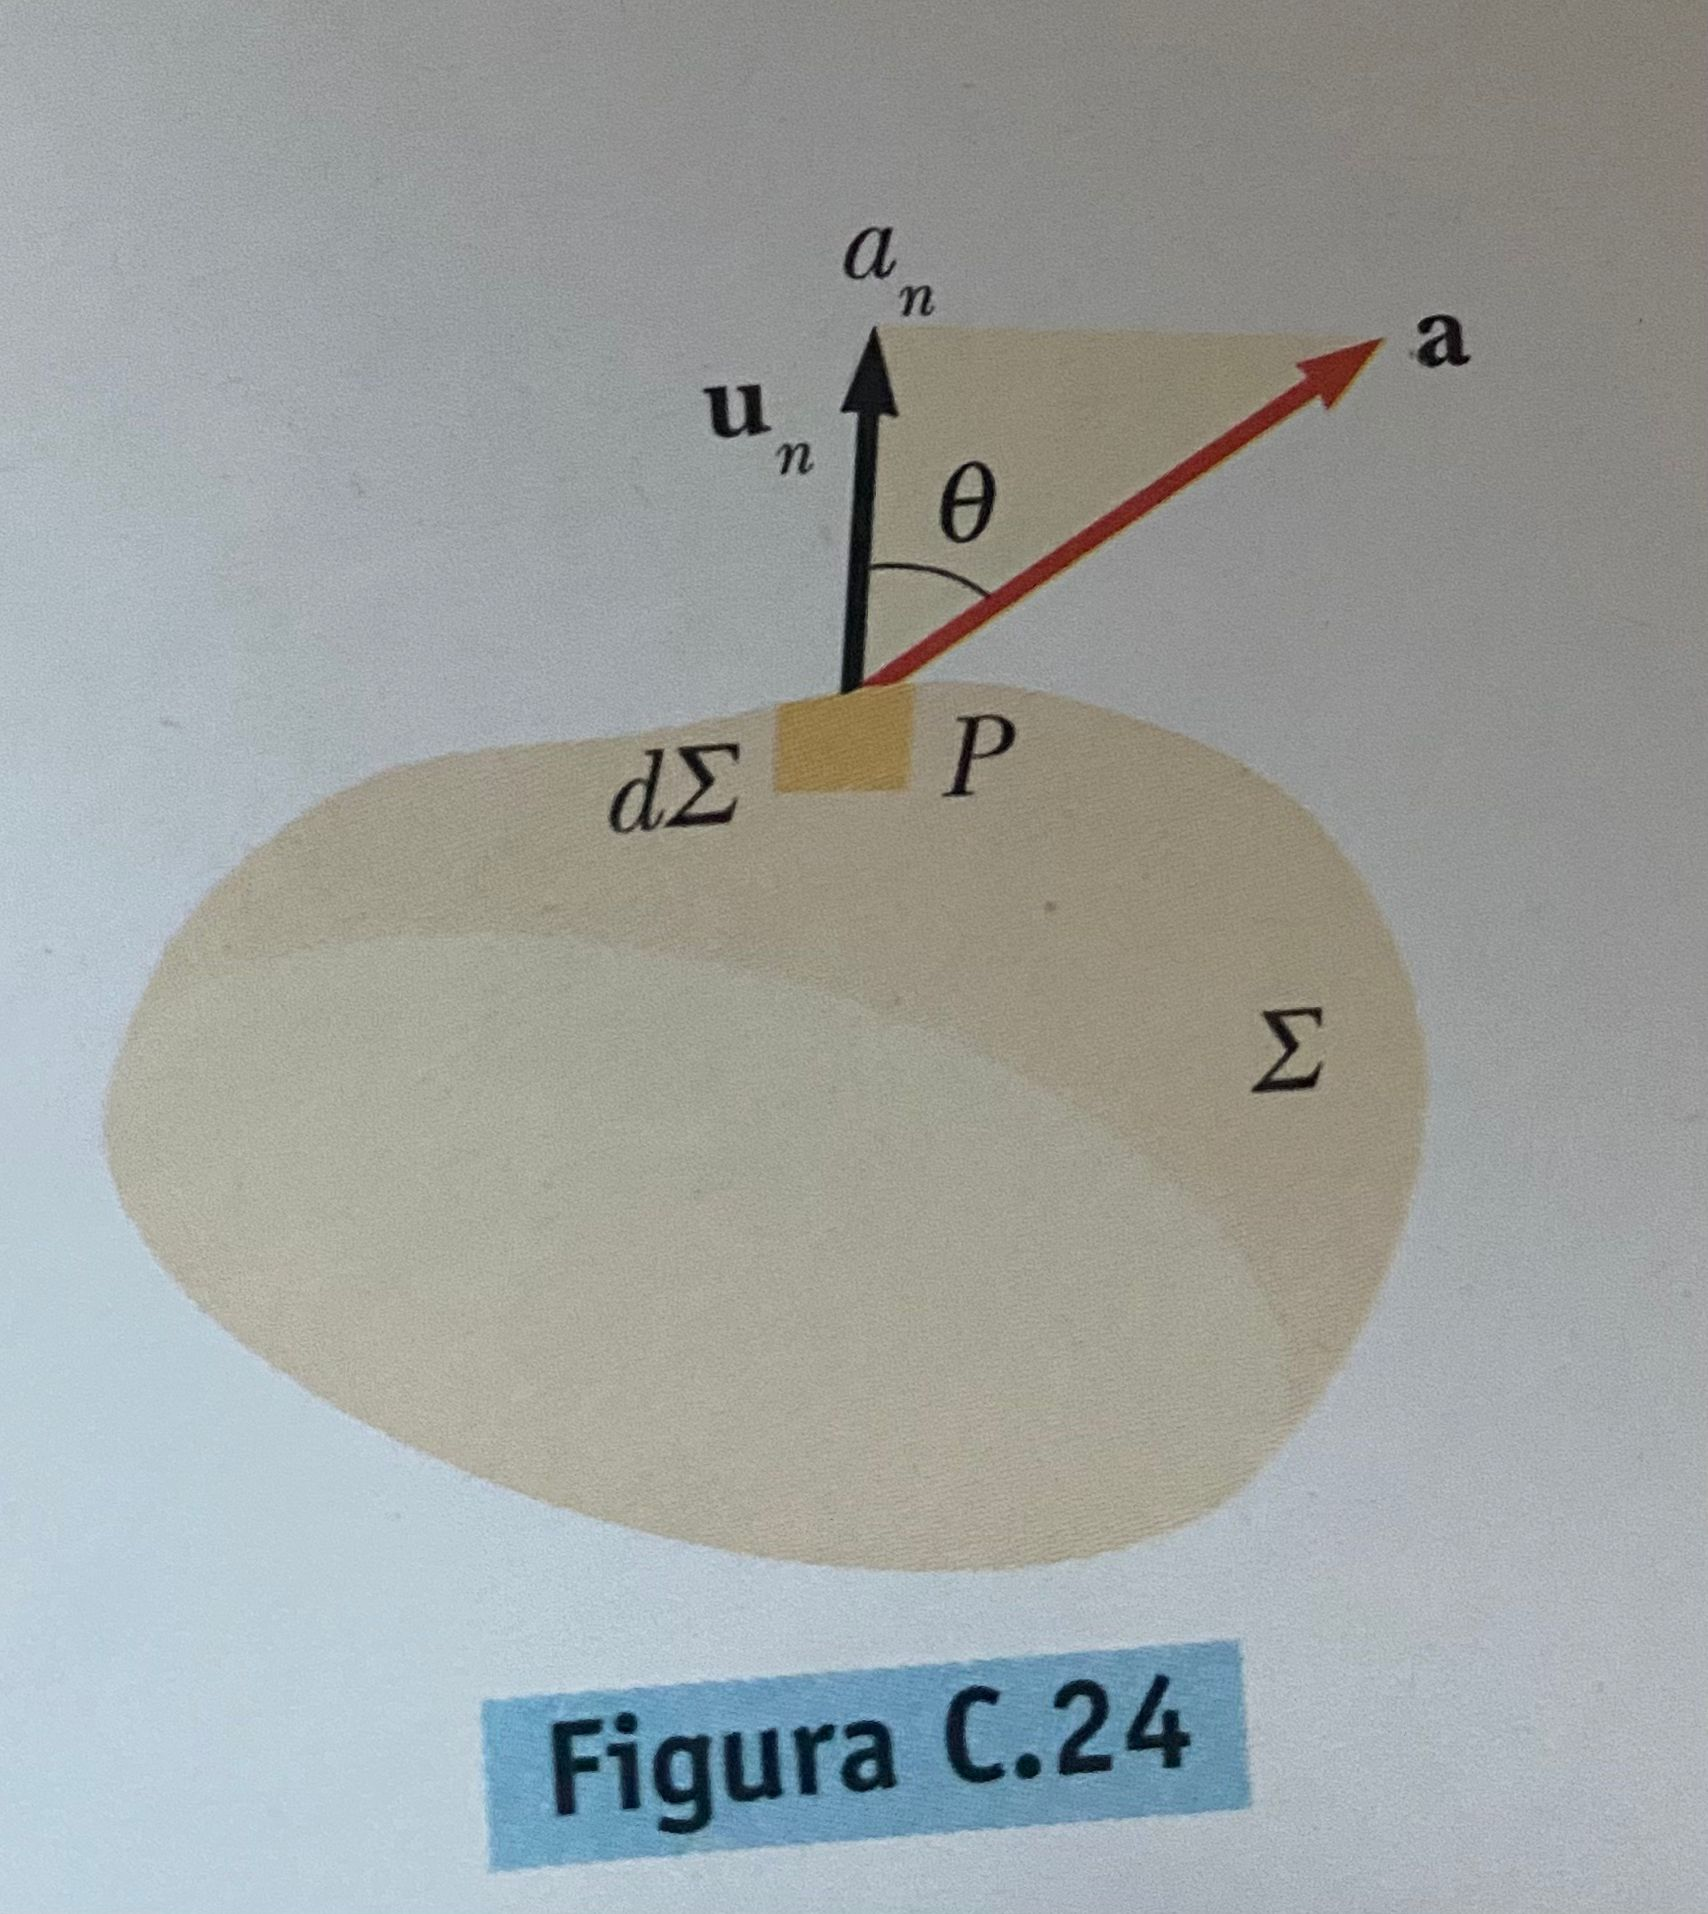
\includegraphics[width=\linewidth]{IntegraleDiSuperficie.jpeg}}
\end{minipage}%
\hfill
\begin{minipage}[t]{0.55\textwidth}
  \raggedright
 Sia $\sum$ una superficie su cui è definito in ciascun punto un vettore a. Considerato
  un elemento di superficie $d \sum$ nell'intorno di un punto P e il versore $u_n$ perpendicolare alla superficie in quel punto, si definisce \textbf{flusso del vettore attraverso d$\sum$} la quantità scalare:
  \begin{equation}
      d \Phi = a \cdot u_n d\sum = a \ d\sum \ cos \theta = a_n d\sum
  \end{equation}
  dove $\theta$ è l'angolo compreso tra a e $u_n$ e $a_s$ è la componente di a normale all'elemento di superficie. Si sommano tutti i flussi infinitesimi ottenuti dalla suddivisione della superficie $\sum$; Il risultato è il flusso totale attraverso $\sum$ che corrisponde all'\textbf{integrale di superficie} del vettore a attraverso la superficie orientata, e si indica con:
  \begin{equation}
      \Phi(a) = \int_ \sum a \cdot u_n d\sum
  \end{equation}
  Se si cambia il verso di $u_n$ cambia il segno del flusso. Se la superficie è chiusa e la si orienta, ad esempio, con la normale in ciascun punto diretta verso l'esterno si ottiene il flusso del vettore a attraverso la superficie chiusa stessa, che si indica:
  \begin{equation}
      \Phi(a)=\oint a \cdot u_n d \sum
  \end{equation}
  \end{minipage}
\section{Cinematica del punto: moto nel piano}
\subsection{Moto nel piano. Posizione e Velocità}
Nel caso che il moto sia vincolato a svolgersi su di un piano la \textbf{traiettoria} del punto P è in generale una \textbf{linea curva}. La descrizione del moto diventa subito più complessa e necessita di un numero maggiore di informazioni rispetto al caso del moto rettilineo. Non basta più specificare il valore numerico dello spostamento, ma occorre precisare in quale direzione sta avvenendo il moto e con quale verso. Grandezze con caratteristiche direzionali oltre che numeriche si chiamano vettori.
\begin{figure}[H] % Usa 'H' per forzare la posizione qui
    \centering % Centra l'immagine
    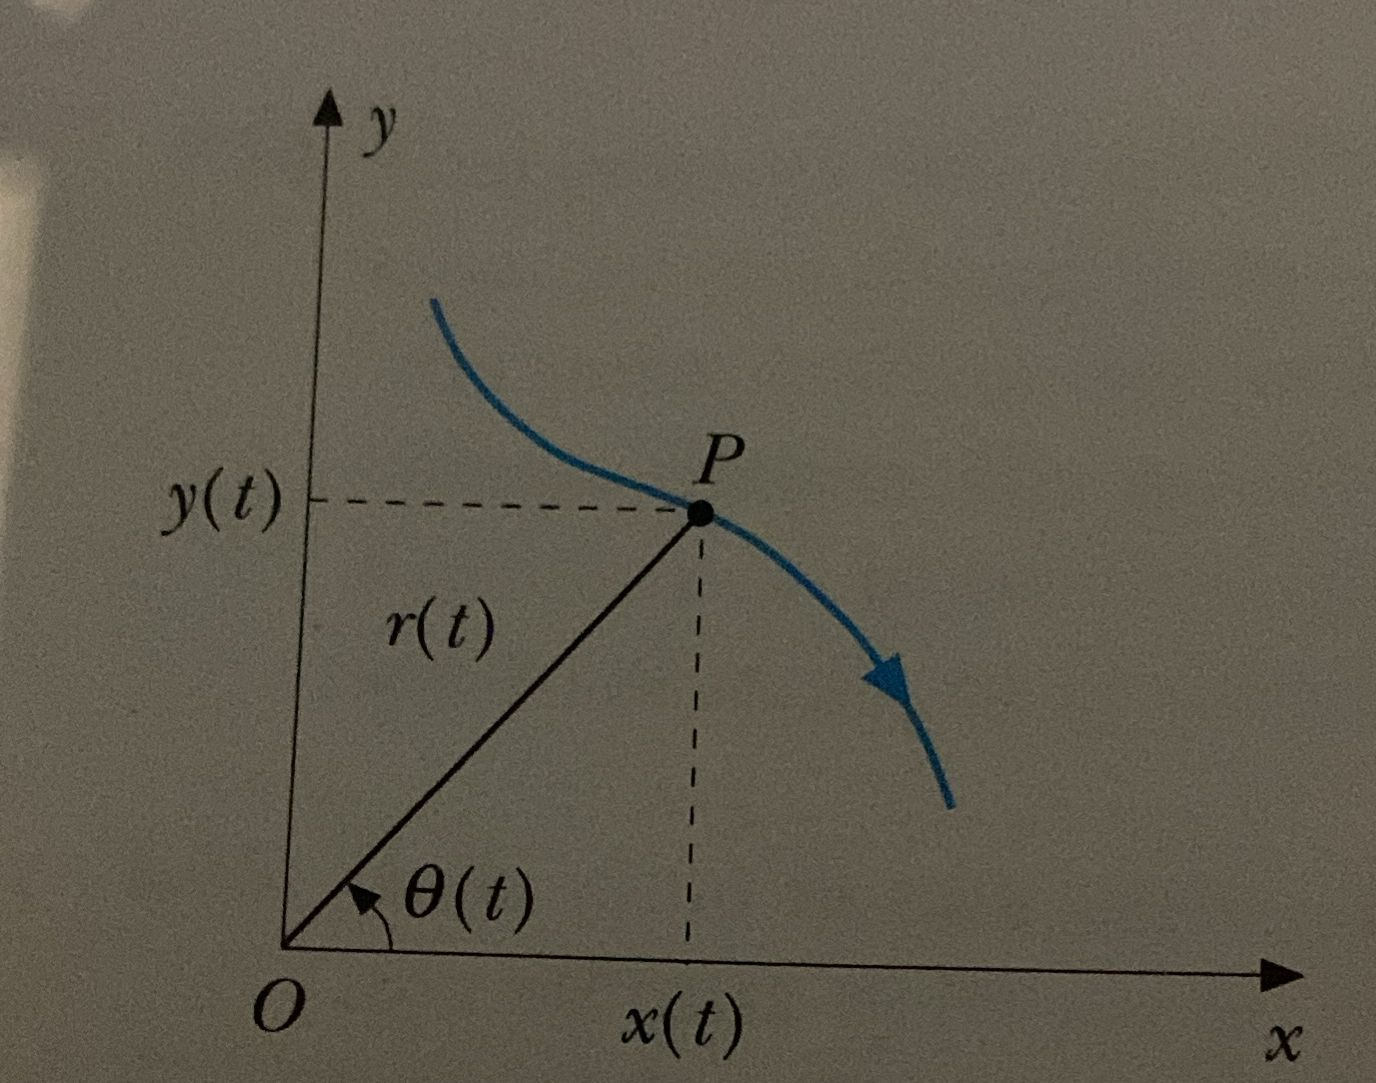
\includegraphics[width=5cm, height=5cm]{TraiettoriaDiUnPuntoInUnPiano.jpeg} % Percorso dell'immagine
    \caption{Traiettoria di un punto in un piano} % Didascalia per l'immagine
    \label{fig:immagine} % Etichetta per riferimento
\end{figure}
\noindent
Tornando al moto su di un piano, la posizione del punto viene individuata da due coordinate. Esse possono essere, con riferimento ad un sistema di asi cartesiani ortogonali, x(t) e y(t) oppure, in termini di coordinate polari nel piano, r(t) e $\theta (t)$. Le relazioni che intercorrono tra le coordinate cartesiane e quelle polari sono, come si deduce subito dalla figura:
\begin{equation}
    x = r cos\theta \ \ , \ \ y= r sen \theta \ \ ; \ \ r = \sqrt{x^2 + y^2} \ \ , \ \ tg \theta =\frac{y}{x}
\end{equation}
La posizione del punto P può anche essere individuata per mezzo del \textbf{raggio vettore} che congiunge l'origine con il punto P:
\begin{equation}
    \vec{r}(t) = OP=x(t)\vec{u}_x + y(t)\vec{u}_y
\end{equation}
dove $u_x$ e $u_y$ rappresentano i \textbf{versori degli assi cartesiani}, che si considerano fissi nel tempo. Se è nota la dipendenza dal tempo di r, cioè la funzione r(t), è individuato il moto nel punto P: conoscere r(t) significa ovviamente dare x(t) e y(t) oppure r(t) e $\theta (t)$; ed è vero viceversa. La posizione del punto lungo la traiettoria può anche essere data da una coordinata curvilinea s, misurata a partire da un'origine arbitraria. Il valore di s esprime la lunghezza della traiettoria e varia nel tempo durante il moto: $ds/dt$ indica la variazione temporale della posizione lungo la traiettoria cioè la velocità istantanea del punto, come definita nel moto rettilineo. Consideriamo due posizioni dal punto P al tempo t e al tempo $ t + \Delta t$: esse sono individuate dai vettori r(t) e $r(t + \Delta t) = r(t) + \Delta r$. Il vettore:
\begin{equation}
    \Delta \vec{r} = \vec{r}(t + \Delta t) - \vec{r}(t)
    \end{equation}
    si chiama \textbf{vettore spostamento} e si definisce \textbf{velocità media} del punto materiale durante l'intervallo di tempo $\Delta t$ il vettore rapporto tra spostamento $\Delta r$ e l'intervallo di tempo stesso necessario per percorrerlo:
    \begin{equation}
        \vec{v}_m = \frac{\Delta \vec{r}}{\Delta t}
    \end{equation}
    Con lo stesso procedimento già utilizzato per il moto rettilineo, si definisce la \textbf{velocità vettoriale}:
    \begin{equation}
        \vec{v}= \frac{d\vec{r}}{dt}
    \end{equation}
    \textbf{La velocità vettoriale è la derivata del raggio vettore rispetto al tempo.}
    \begin{figure}[H] % Usa 'H' per forzare la posizione qui
    \centering % Centra l'immagine
    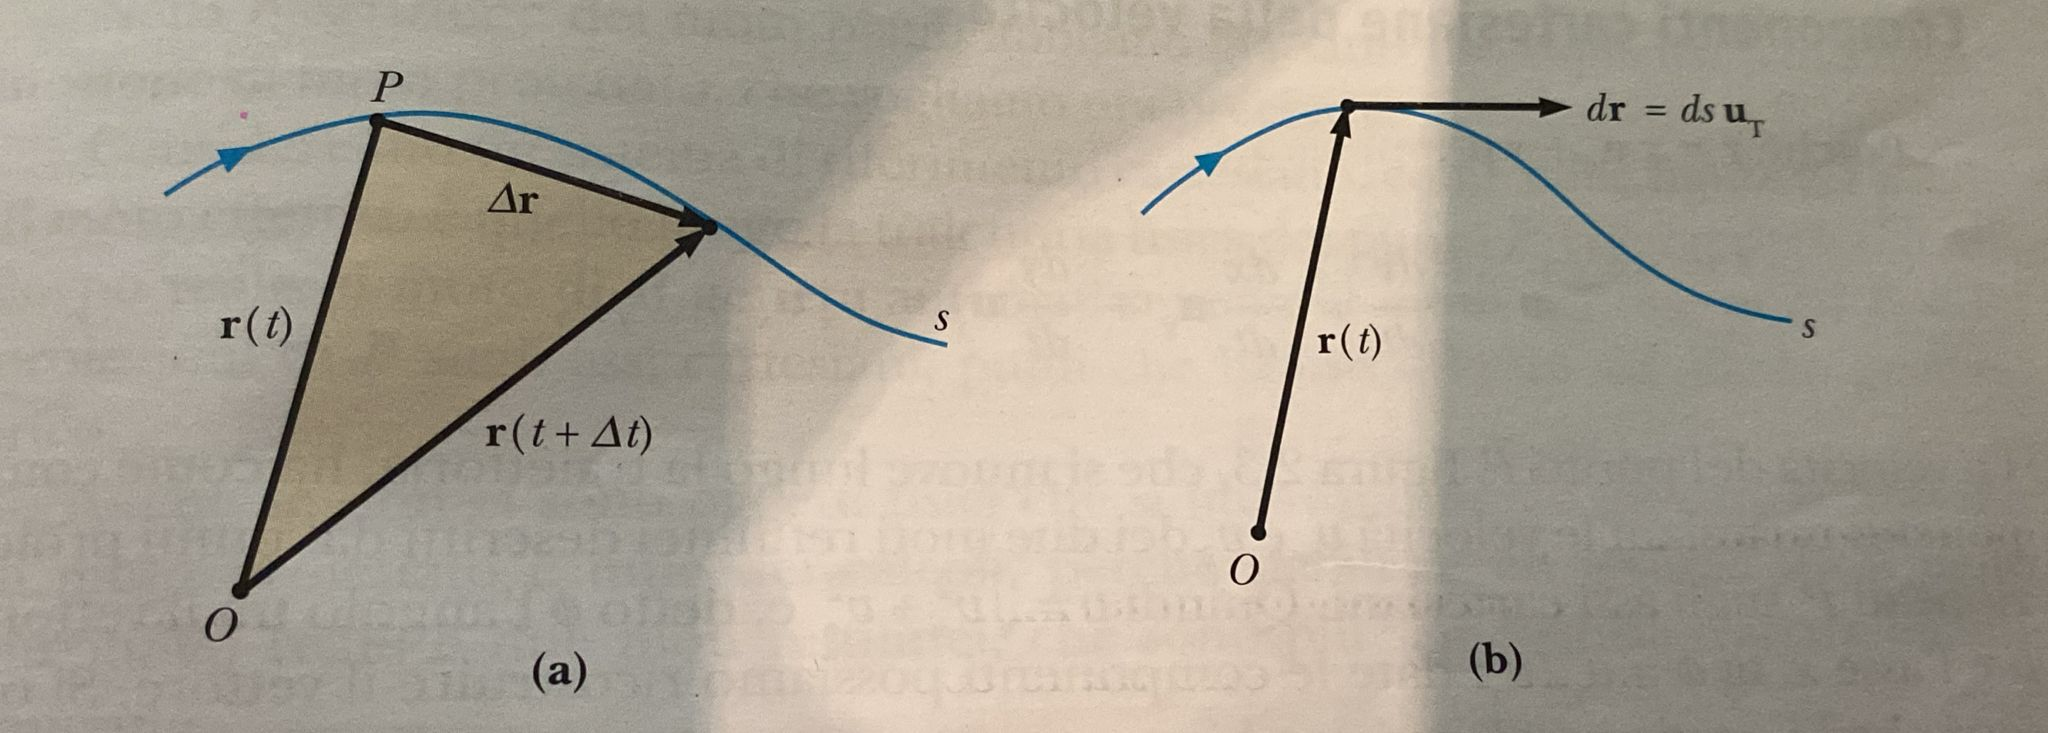
\includegraphics[width=7cm, height=3cm]{VelocitàVettoriale.jpeg} % Percorso dell'immagine
    \caption{Spostamento finito (a) e spostamento infinitesimo di un punto (b) su una traiettoria piana} % Didascalia per l'immagine
    \label{fig:immagine} % Etichetta per riferimento
\end{figure}
\noindent
Osserviamo, figura da 13b, che al limite l'incremento dr del raggio vettore risulta in direzione tangente alla traiettoria nel punto P e in modulo eguale allo spostamento infinitesimo ds lungo la traiettoria, per cui possiamo scrivere $dr=dsu_T$ dove $u_T$ è il versore della tangente alla curva, variabile nel tempo man mano che il punto avanza lungo la traiettoria. In sostanza pensiamo il moto come una successione di spostamenti rettilinei infinitesimi con direzione variabile: la direzione istantanea del moto coincide con quella della tangente alla traiettoria nel punto occupato all'istante considerato. Quindi:
\begin{equation}
    \vec{v} = \frac{ds}{dt}\vec{u}_T = v\vec{u}_T
\end{equation}
pertanto la velocità vettoriale v individua in ogni istante con la sua direzione e verso la direzione e il verso del moto con il suo modulo $v=\frac{ds}{dt}$ la velocità istantanea con cui è percorsa la traiettoria. Si faccia attenzione a non confondere i due concetti, raggio vettore e i suoi incrementi finiti da una parte, percorso effettivo dall'altra. La traiettoria del moto e il fatto che la velocità si scrive $vu_T$ sono caratteristiche intrinseche, che cioè non dipendono dalla scelta del sistema di riferimento.
\subsubsection{Componenti cartesiane della velocità}
Poichè $r=xu_x + yu_y$:
\begin{equation}
    \vec{v} = \frac{d\vec{r}}{dt}=\frac{dx}{dt}\vec{u}_x + \frac{dy}{dt}\vec{u}_y=v_x\vec{u}_x+v_y\vec{u}_y
\end{equation}
\subsubsection{Componenti polari della velocità}

  \begin{minipage}[t]{0.4\textwidth}
  \raisebox{-\height}{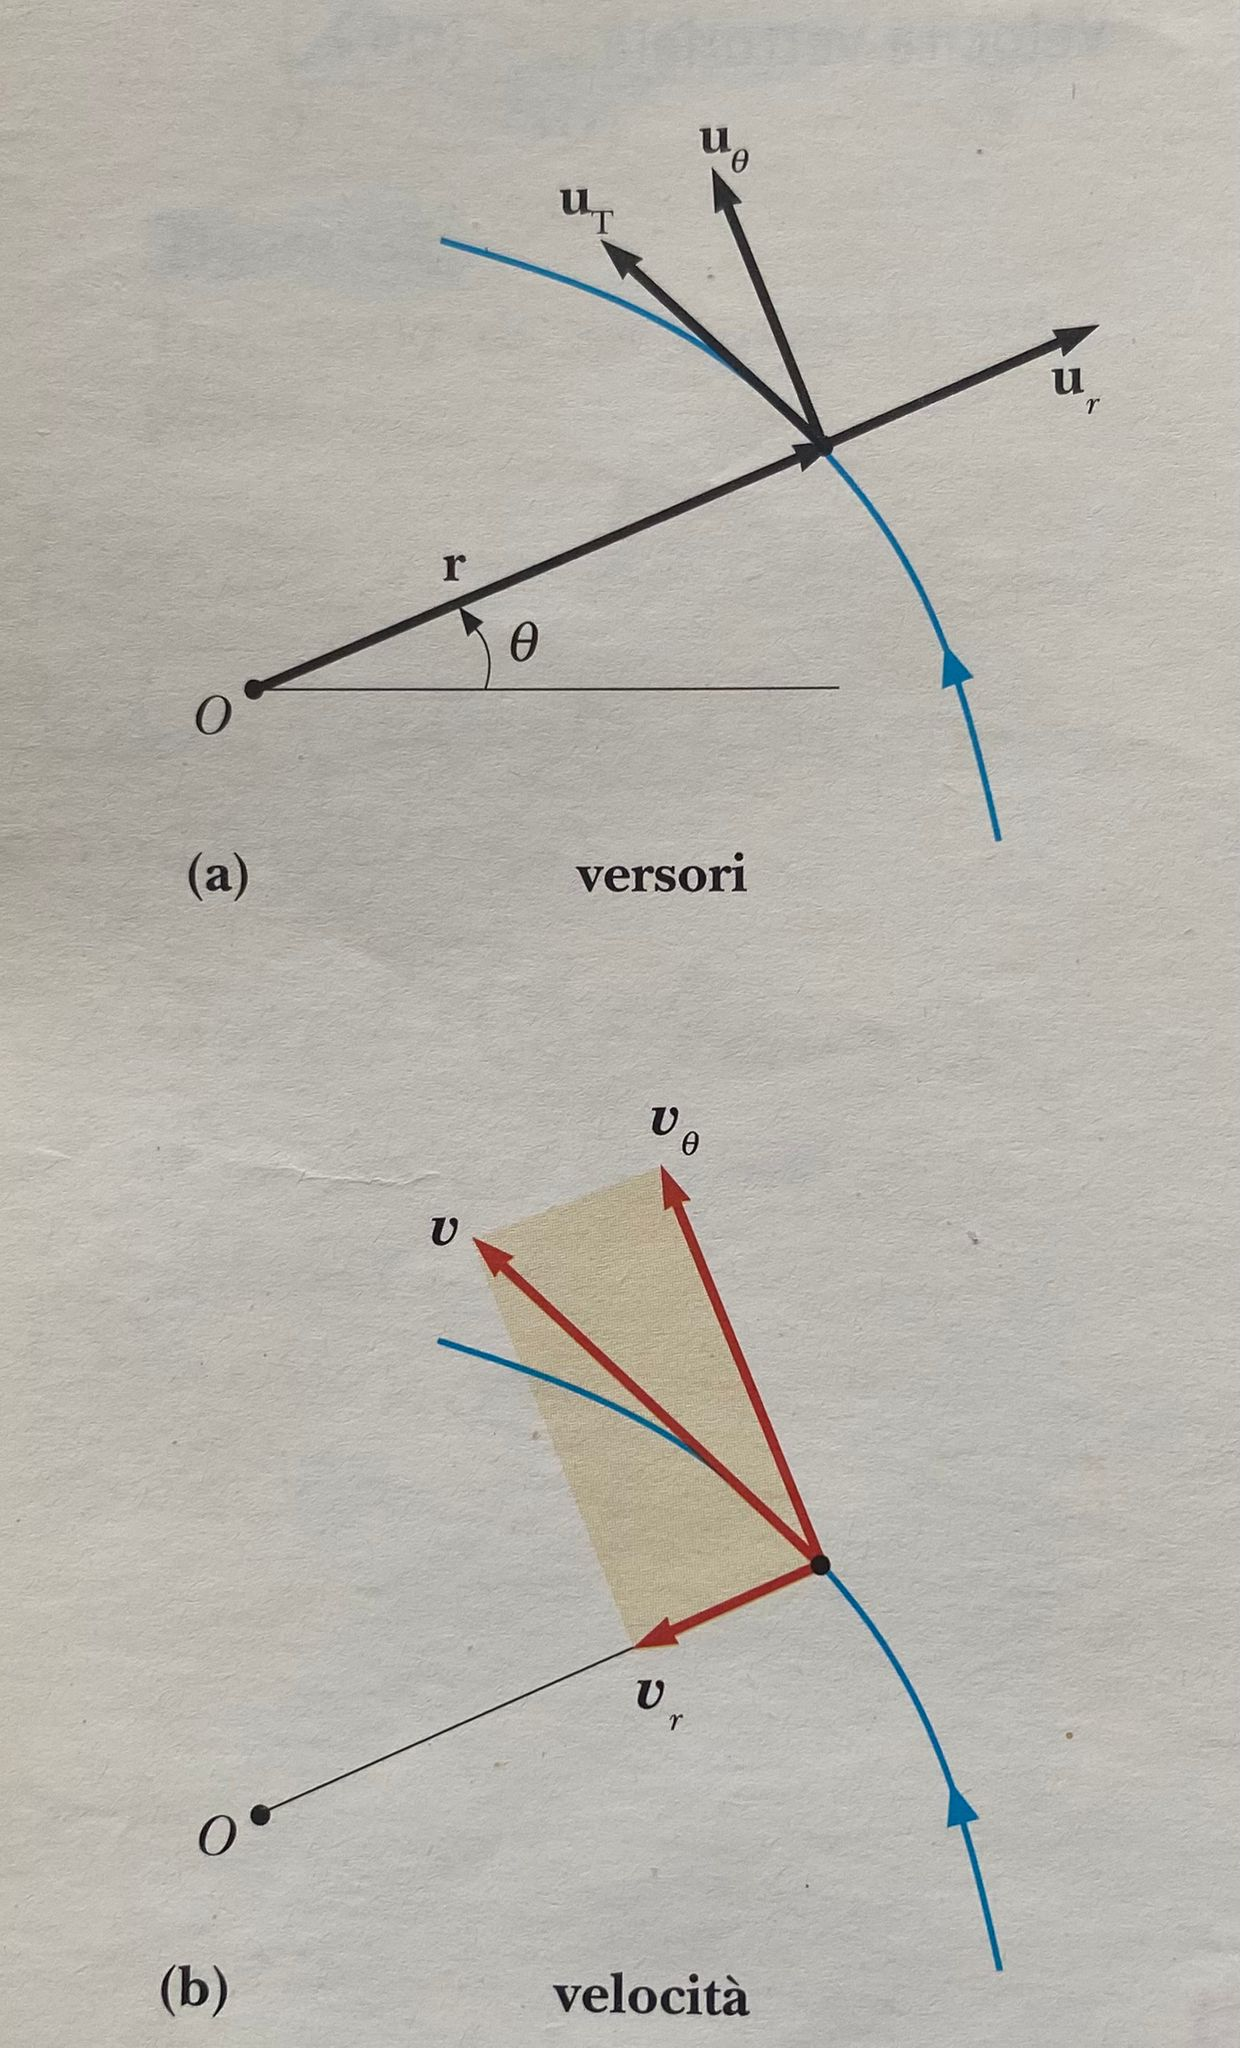
\includegraphics[width=\linewidth]{CoordinatePolari.jpg}}
\end{minipage}%
\hfill
\begin{minipage}[t]{0.55\textwidth}
  \raggedright
Introduciamo i vettori $u_r$ e $u_\theta$, rispettivamente versore della direzione di r e versore ortogonale alla stessa; si noti che questi versori cambiano direzione (ruotano) durante il moto. Il raggio vettore r può essere espresso come $ru_r$ e pertanto:
\begin{equation}
    \vec{v}=\frac{d\vec{r}}{dt}=\frac{dr}{dt}\vec{u}_r + r\frac{d\vec{u}_r}{dt} \ -> \ \vec{v}=\frac{dr}{dt}\vec{u}_r + r\frac{d \theta}{dt}\vec{u}_\theta = \vec{v}_r + \vec{v}_\theta
\end{equation}
La velocità che, si ricordi, è sempre tangente alla traiettoria si scompone in due componenti: la \textbf{velocità radiale $v_r$}, diretta lungo r e di modulo $\frac{dr}{dt}$ e la \textbf{velocità traversa $v_\theta$}, ortogonale a r e di modulo $rd\theta/dt$; $v_r$ dipende dalle variazioni del modulo del raggio vettore, $v_\theta$ è collegata alle variazioni di direzione dello stesso. Il modulo della velocità è, con queste componenti:
\begin{equation}
    v=\frac{ds}{dt}= \sqrt{(\frac{dr}{dt})^2 + r^2(\frac{d\theta}{dt})^2}
\end{equation}
In definitiva abbiamo mostrato come si determina la velocità se è nota la posizione, in coordinate cartesiane o polari.
\begin{equation}
    \vec{r}(t)=\vec{r}(t_0) + \int_{t_0}^t \vec{v}(t) dt
\end{equation}
  \end{minipage}
\subsubsection{Moto reale e moti proiettati}
Consideriamo un sistema di riferimento cartesiano. Il moto effettivo è quello lungo la traiettoria fisica del punto P che rappresenta un corpo reale; il moto di P genera automaticamente il moto dei due punti $P_x$ e $P_y$ proiezioni di P sugli assi cartesiani, punti che hanno solo un significato geometrico. Anche se non ci sono oggetti fisici che si muovono lungo gli assi, la nozione di moto proiettato è utile nei calcoli, perchè stabilisce un legame tra il moto curvilineo reale e due moti rettilinei, che sono più semplici da trattare analiticamente.
\newpage
\subsection{Accelerazione nel moto piano}
L'accelerazione nel moto piano deve esprimere le variazioni della velocità sia come modulo he direzione e quindi ci aspettiamo che abbia due componenti, una legata alla variazione del modulo della velocità e la seconda al cambiamento di direzione del moto.
\begin{figure}[H] % Usa 'H' per forzare la posizione qui
    \centering % Centra l'immagine
    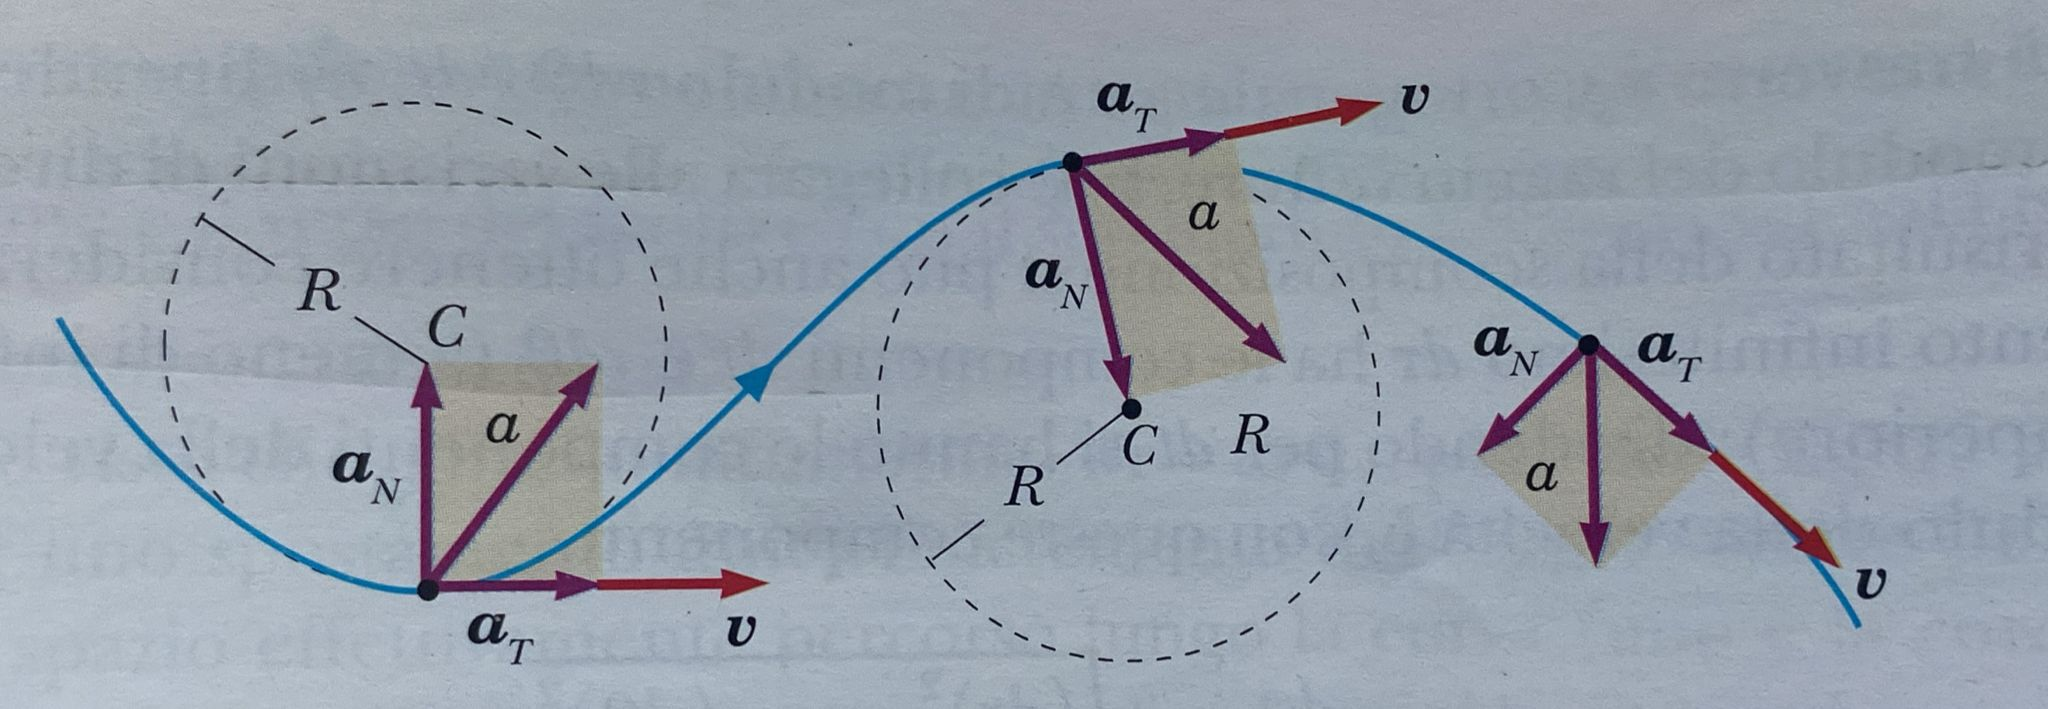
\includegraphics[width=8cm, height=3cm]{AccelerazioneVettoriale.jpg} % Percorso dell'immagine
    \caption{Componenti dell'accelerazione di un punto lungo una traiettoria piana.} % Didascalia per l'immagine
    \label{fig:immagine} % Etichetta per riferimento
\end{figure}
\noindent
Si definisce l'\textbf{accelerazione vettoriale}:
\begin{equation}
    \vec{a}=\frac{d\vec{v}}{dt}=\frac{d^2\vec{r}}{dt^2}
\end{equation}
come derivata della velocità vettoriale rispetto al tempo o come derivata seconda del vettore spostamento rispetto al tempo. Utilizziamo la 3.1.6 e la regola di derivazione di un vettore:
\begin{equation}
    \vec{a}= \frac{d}{dt}(v\vec{u}_T) = \frac{dv}{dt}\vec{u}_T + v\frac{d\vec{u}_T}{dt} = \frac{dv}{dt}\vec{u}_T + v\frac{d\phi}{dt}\vec{u}_N
\end{equation}
La prima componente, parallela alla velocità e quindi tangente alla traiettoria, esprime la variazione del modulo della velocità. Il secondo termine, dipendente dalla variazione di direzione della velocità, è ortogonale a questa: $u_N$ è un vettore ortogonale a $u_T$ diretto verso la concavità della traiettoria, e $d\phi/dt$ dicce quanto rapidamente cambia la direzione di $u_T$ e quindi di $u_N$.
\begin{minipage}[t]{0.4\textwidth}
  \raisebox{-\height}{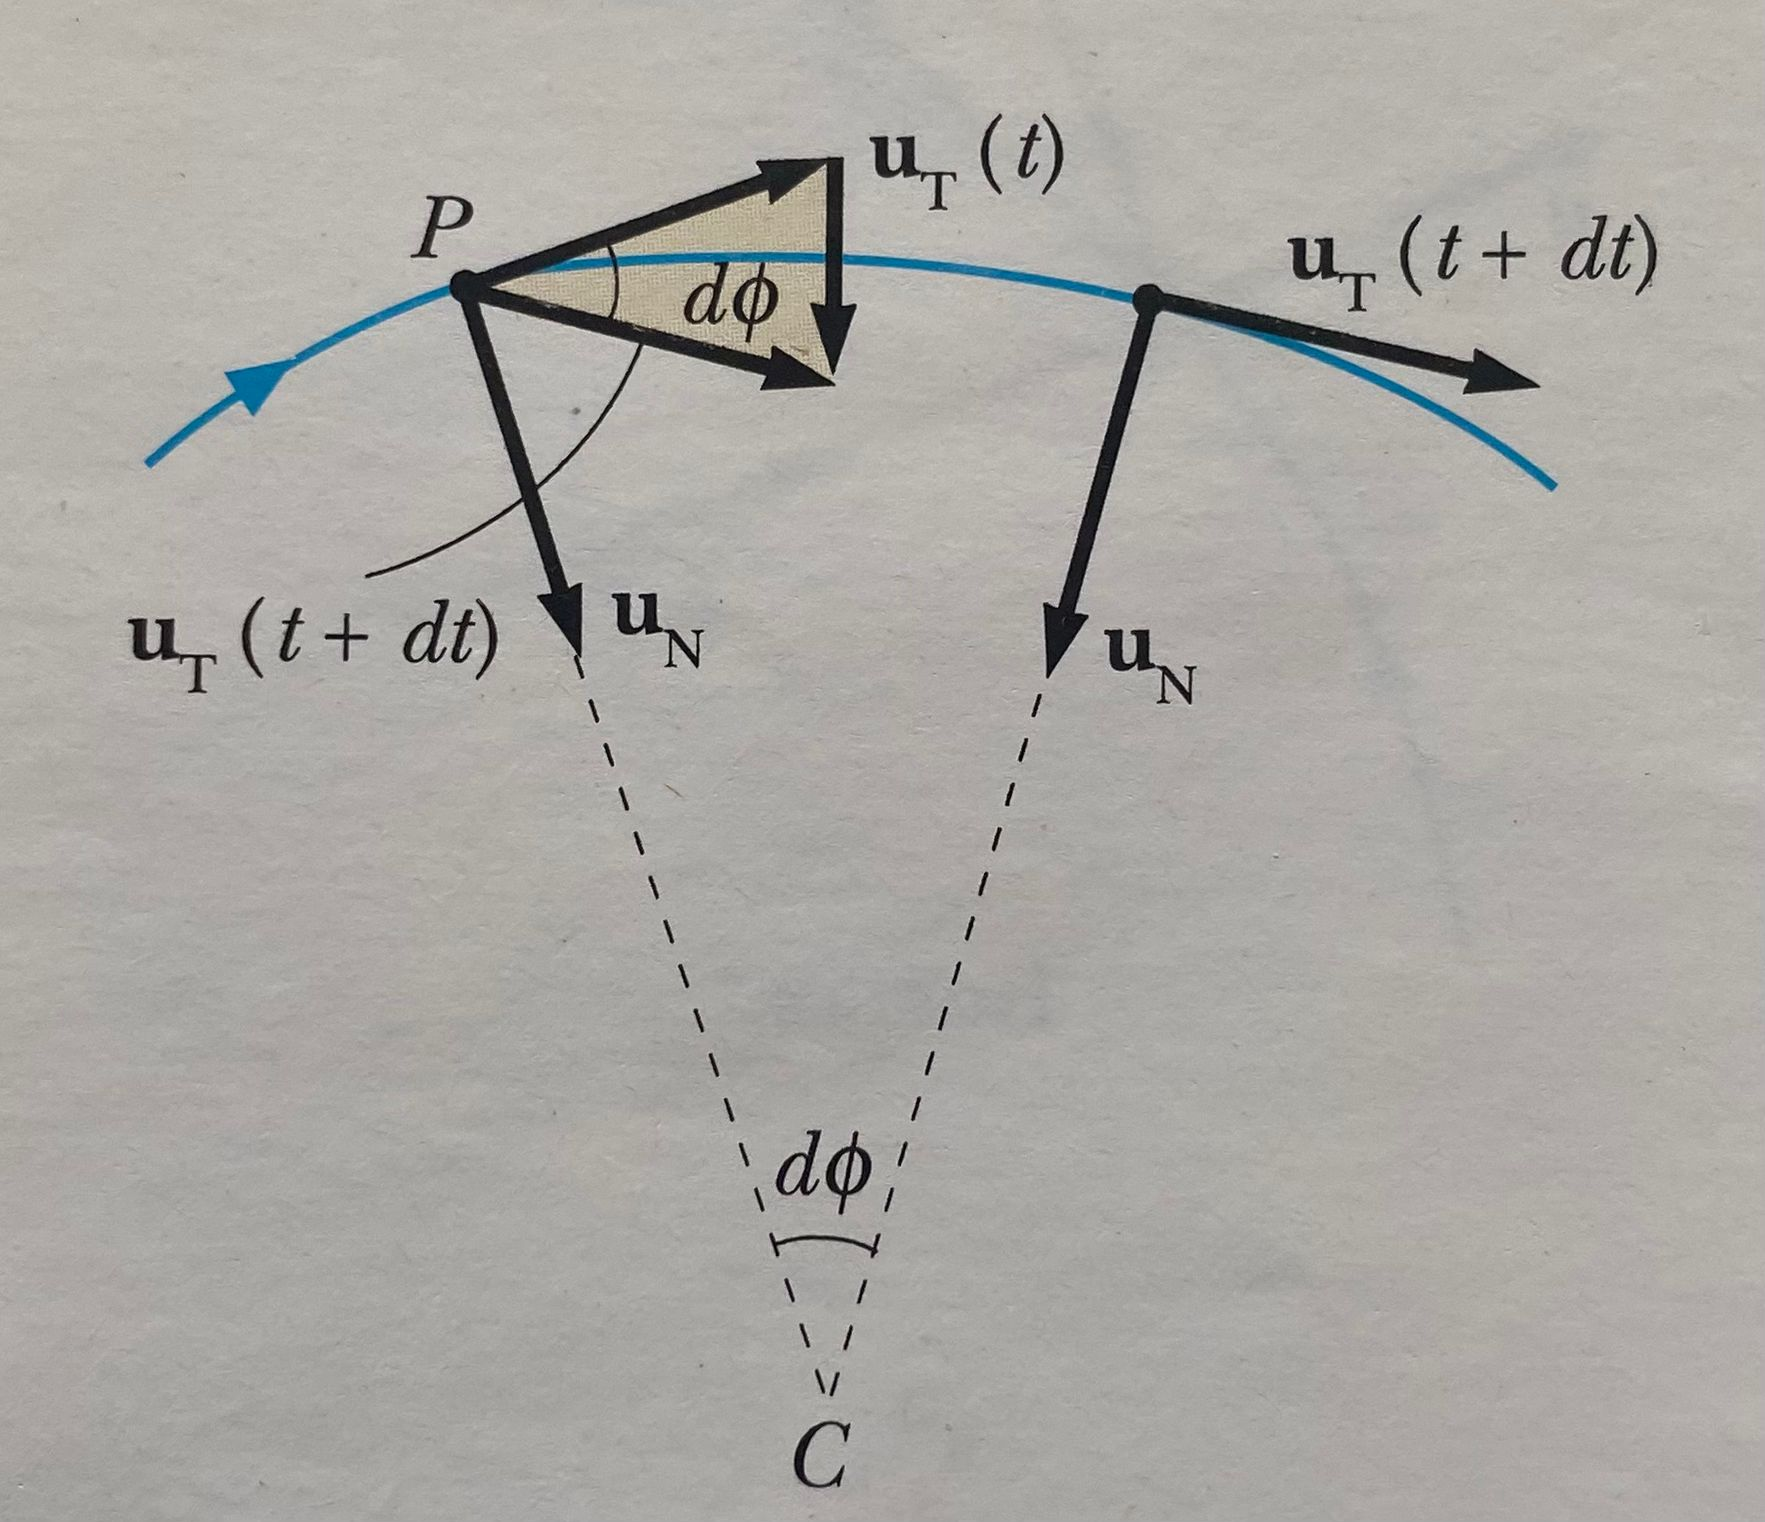
\includegraphics[width=\linewidth]{ComponenteNormaleDell'Accelerazione.jpg}}
\end{minipage}%
\hfill
\begin{minipage}[t]{0.55\textwidth}
  \raggedright
Le rette normali alla traiettoria in due punti molto vicini tra lori si incontrano nel punto C, che coincide con il centro della circonferenza tangente alla traiettoria nel punto P e si chiama anche \textbf{centro di curvatura} della traiettoria nel punto P. Al variare di P lungo la traiettoria variano sia il valore di R che la posizione di C. L'arco di traiettoria ds è pari a $Rd\phi$ con $R=CP$ \textbf{raggio di curvatura}.
\begin{equation}
    \vec{a}=\frac{dv}{dt}\vec{u}_T + \frac{v^2}{R}\vec{u}_N=\vec{a}_T+\vec{a}_N
\end{equation}
\begin{equation}
    |a|=\sqrt{a_T^2+a_N^2}=\sqrt{(\frac{dv}{dt})+\frac{v^4}{R^2}}
\end{equation}
Le due componenti si chiamano \textbf{accelerazione tangenziale} e \textbf{accelerazione normale} o \textbf{centripeta}. In un moto curvilineo vario entrambe le componenti sono diverse da zero; se però il moto curvilineo è uniforme è nulla $a_T$. Invece nel moto rettilineo vario è nulla $a_N$ e solo nel moto rettilineo uniforme $a_T=a_N=0$.
  \end{minipage}
  \subsubsection{Componenti cartesiane dell'accelerazione}
  Le componenti cartesiane dell'accelerazione sono le accelerazioni dei due moti rettilinei proiezioni sugli assi del moto di P lungo la traiettoria curva:
  \begin{equation}
      \vec{a}=\frac{d\vec{v}}{dt}=\frac{dv_x}{dt}\vec{u}_x+\frac{dv_y}{dt}\vec{u}_y=\frac{d^2x}{dt^2}\vec{u}_x + \frac{d^2y}{dt^2}\vec{u}_y=a_x\vec{u}_x+a_y\vec{u}_y
  \end{equation}
  Se $\phi$ è l'angolo che $u_T$ forma con $u_x$:
  \begin{align}
     & a_x=\frac{dv}{dt}cos\phi-\frac{v^2}{R}sen\phi \\
     & a_y=\frac{dv}{dt}sen\phi-\frac{v^2}{R}cos\phi \\
     & \vec{v}(t) = \vec{v}(t_0) + \int_{t_0}^t \vec{a}(t)dt
  \end{align}
\subsection{Moto Circolare}
Si chiama \textbf{moto circolare} un moto piano la cui traiettoria è rappresentata da una circonferenza. Considerando che la velocità varia continuamente in direzione l'\textbf{accelerazione centripeta è sempre diversa da 0} (e quindi agisce una forza detta centripeta, diretta verso il centro della circonferenza). Nel moto circolare uniforme la velocità è costante in modulo e l'accelerazione tangente è nulla per cui $a=a_N$; se invece il modulo della velocità cambia nel tempo, il moto circolare non è uniforma e $a_T$ è diversa da zero. Il moto circolare può essere descritto facendo riferimento allo spazio percorso sulla circonferenza s(t) oppure utilizzando l'angolo $\theta (t)$ sotteso dall'arco s(t), con $\theta (t)= s(t)/R$. Introduciamo lo \textbf{spostamento angolare}:
\begin{equation}
    \Delta \theta= \theta_2 - \theta_1
\end{equation}
  Si definisce \textbf{velocità angolare media} il rapporto tra $\Delta \theta $ e $\Delta t$:
  \begin{equation}
      \omega_m=\frac{\Delta \theta}{\Delta t}
  \end{equation}
  La \textbf{velocità angolare istantanea} è definita come:
  \begin{equation}
      \omega=\frac{d \theta}{dt}
  \end{equation}
  La velocità angolare istantanea è la derivata rispetto al tempo dell'angolo $\theta (t)$ che descrive la posizione angolare del punto. Tenendo conto di $s(t)= R \theta(t)$:
  \begin{equation}
      \omega = \frac{d \theta}{dt}= \frac{1}{R}\frac{ds}{dt}=\frac{v}{R}
  \end{equation}
  \textbf{La velocità angolare è proporzionale alla velocità con cui è descritta la circonferenza.} Nel moto circolare la velocità radiale è nulla. Il \textbf{moto circolare} più semplice è quello \textbf{uniforme}: $v \ e \ \omega$ sono costanti e le leggi orarie, con riferimento alle due variabili utilizzate si scrivono:
  \begin{align}
      & s(t)=s_0 + vt \\
      & \theta(t)= \theta_0 + \omega t
  \end{align}
  Il \textbf{moto circolare uniforme è un moto accelerato con accelerazione costante, ortogonale alla traiettoria}.
  \begin{equation}
      a=a_N=\frac{v^2}{R}=\omega^2R
  \end{equation}
  Ovviamente il moto è periodico. Nel caso del \textbf{moto circolare non uniforme} oltre all'accelerazione centripeta, che è variabile perchè la velocità varia anche in modulo, dobbiamo considerare l'accelerazione tangenziale $a_T= dv/dt$. Dato che varia anche la velocità angolare $\omega$ occorre considerare l'\textbf{accelerazione angolare media}:
  \begin{equation}
      \alpha_m=\frac{\Delta \omega}{\Delta t}
  \end{equation}
  L'\textbf{accelerazione angolare istantanea}:
  \begin{equation}
      \alpha=\frac{d \omega}{dt}=\frac{d^2 \theta}{dt^2}=\frac{1}{R}\frac{dv}{dt}=\frac{a_T}{R}
  \end{equation}
  Di conseguenza:
  \begin{align}
      & \omega (t)= \omega_0 + \int_{t_0}^t \alpha(t) dt \\
      & \theta (t)= \theta_0 + \int_{t_0}^t \omega(t) dt
  \end{align}
  Un caso particolare di moto circolare non uniforme è costituito dal \textbf{moto circolare uniformemente accelerato} in cui $\alpha = costante$ ovvero $a_T=costante$.
  \begin{align}
      & \omega = \omega_0 + \alpha t \\
      & \theta = \theta_0 + \omega_0t + \frac{1}{2}\alpha t^2 \\
      & a_N = \omega^2R=(\omega_0+\alpha t)^2R
  \end{align}
  In caso in cui abbiamo $\alpha (\theta)$:
  \begin{equation}
      \int_{\theta_0}^\theta \alpha(\theta)d\theta= \frac{1}{2}\omega^2-\frac{1}{2}w_0^2
  \end{equation}
  \subsubsection{Notazione vettoriale}
  \begin{align}
      &  \vec{v}= \vec{\omega} \times \vec{r} \\
      &  \vec{a} = \vec{\alpha} \times \vec{r} + \vec{\omega} \times \vec{v}
  \end{align}
Il primo termine è \textbf{l'accelerazione tangenziale $a_T$}, il secondo è l'\textbf{accelerazione centripeta $a_N$}.
\subsection{Moto Parabolico dei Corpi}
Vogliamo determinare in un moto parabolico: la \textbf{traiettoria}, la \textbf{massima altezza} raggiunta e la posizione G in cui il punto ricade sull'asse x ovvero la \textbf{gittata} OG. Il moto è caratterizzato da un'accelerazione costante $a=g=-|g|u_y$e al tempo di lancio, $t=0$ abbiamo $r=0 \ e \ v=v_0$. 
\begin{figure}[H] % Usa 'H' per forzare la posizione qui
    \centering % Centra l'immagine
    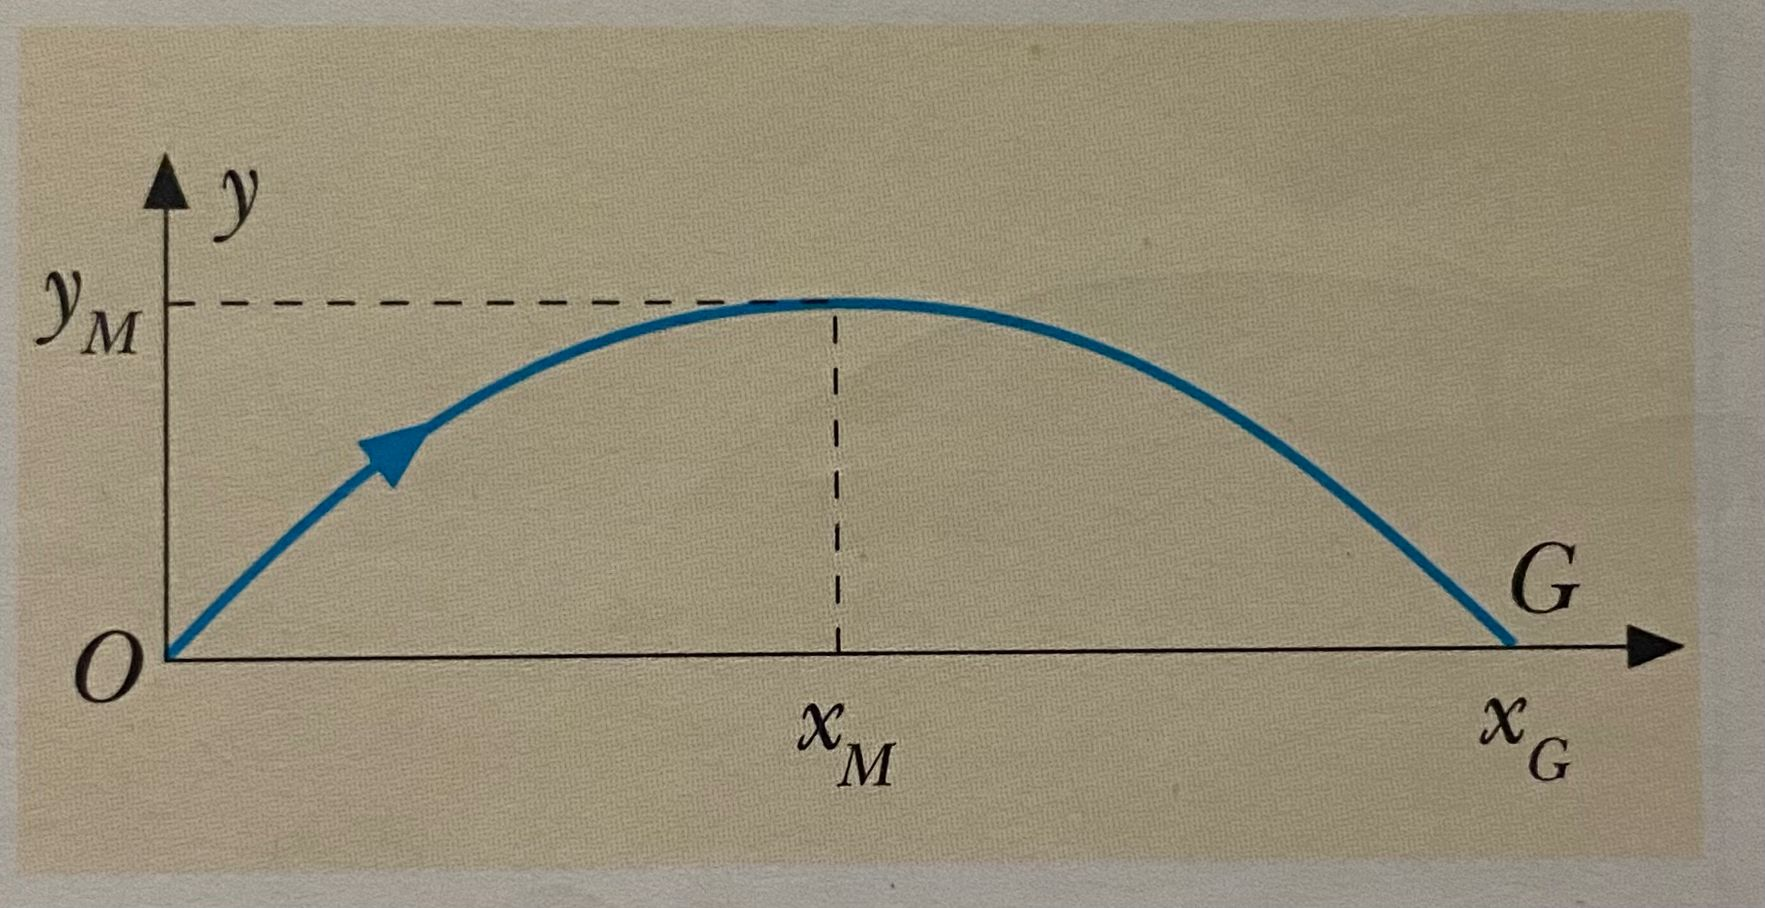
\includegraphics[width=5cm, height=3cm]{motoParabolico.png} % Percorso dell'immagine
    \caption{Traiettoria parabolica di un punto} % Didascalia per l'immagine
    \label{fig:immagine} % Etichetta per riferimento
\end{figure}
\noindent
La traiettoria seguita, equivale all'equazione di una \textbf{parabola}:
\begin{equation}
    y(x)=xtg \theta-\frac{g}{2v_0cos^2\theta}x^2
\end{equation}
 Per quanto riguarda la \textbf{gittata} OG:
 \begin{equation}
     x_G=\frac{v_0^2sen2\theta}{g}=2x_M
 \end{equation}
 Per cui l'altezza massima:
 \begin{equation}
     y(x_M)=y_M= \frac{v_0^2sen\theta}{2g}
 \end{equation}
  L'altezza massima la possiamo ottenere anche eguagliando la traiettoria a 0, trovando $x_M$ e si calcola poi $y(x_M)$. Il \textbf{tempo totale di volo $t_G$} è pari al tempo impiegato a percorrere OG con velocità costante $v_x=v_0cos \theta$:
  \begin{equation}
      t_G= 2x_M/v_0cos \theta=2v_0sen \theta/g=2 t_M
  \end{equation}
  evidentemente $t_G$ coincide con il tempo necessario per salire all'altezza $y_M$ e ritornare al suolo. Notiamo infine che nella posizione G la velocità è la stessa in modulo che alla partenza, ma è posta simmetricamente rispetto all'asse x:
  \begin{equation}
      v_x(t_G)=v_0cos \theta \ , \ v_y(t_G) = -v_0 sen \theta \ , \ tg\phi = -tg \theta
  \end{equation}
  In conclusione, nella trattazione di un moto parabolico il sistema cartesiano è il più semplice da utilizzare, mentre in un moto circolare è più semplice servirsi di un sistema di coordinate polari.
  \subsection{Moto nello spazio}
  Questo moto tridimensionale può essere rappresentato, in coordinate cartesiane, come la somma di tre moti rettilinei lungo gli assi di riferimento per cui scriviamo:
  \begin{align}
      & \vec{r}(t)=x(t)\vec{u}_x + y(t)\vec{u}_y + z(t)\vec{u}_z \\
      & v(t)= v_x\vec{u}_x +v_y\vec{u}_y + v_z\vec{u}_z \\
      & a(t) = a_x\vec{u}_x+a_y\vec{u}_y+a_z\vec{u}_z
  \end{align}
  \subsection{Moto relativo nel piano}
  La \textbf{Posizione relativa di $P_2$ rispetto a $P_1$}:
  \begin{equation}
      \vec{r}_{1,2}(t)=\vec{r}_2(t)-\vec{r}_1(t) 
  \end{equation}
    La \textbf{velocità relativa di $P_2$ rispetto a $P_1$}:
    \begin{equation}
        \vec{v}_{1,2}(t)=\vec{v}_2(t)-\vec{v}_1(t)
    \end{equation}
 L'\textbf{accelerazione relativa di $P_2$ rispetto a $P_1$}:
 \begin{equation}
     \vec{a}_{1,2}(t)=\vec{a}_2-\vec{a}_1
 \end{equation}
 \section{Dinamica del punto: le leggi di Newton}
 \subsection{Principio d'inerzia. Introduzione al concetto di forza}
 La questione fondamentale è perchè avviene il moto, quali sono le cause fisiche per cui un corpo entra in movimento e descrive un certo tipo di moto invece che un altro. La parte della meccanica che si occupa di questo e contiene anche il caso dell'equilibrio statico, cioè lo studio delle condizioni per cui un punto resta in quiete viene detta \textbf{dinamica del punto}. Introduciamo il \textbf{principio d'inerzia (prima legge di Newton)}: \\\\
 Un corpo non soggetto a forze non subisce cambiamenti di velocità, ovvero resta in stato di quiete se era fermo (v=0) oppure si muove di moto rettilineo uniforme (v costante non nulla).\\\\
 \textbf{L'assenza di forza non implica che non ci sia moto, bensì copmporta che la velocità non vari.} Legge quantitativa:\\
 La variazione di velocità, in modulo in direzione o in entrambi, di un corpo è dovuta all'azione di una forza.\\
 Dato che il principio d'inerzia richiede, in caso di moto, che questo sia rettilineo uniforme, un \textbf{moto accelerato segnala la presenza di una forza agente}. Non è necessario un contatto per esercitare una forza. Dunque: \textbf{la forza è la grandezza che esprime e misura l'interazione tra sistemi fisici.} Intuitivamente possiamo affermare che alla forza è associata la nozione di intensità e di direzionalità. L'effetto di una forza cambia con la direzione. \\\\
 \begin{minipage}[t]{0.4\textwidth}
  \raisebox{-\height}{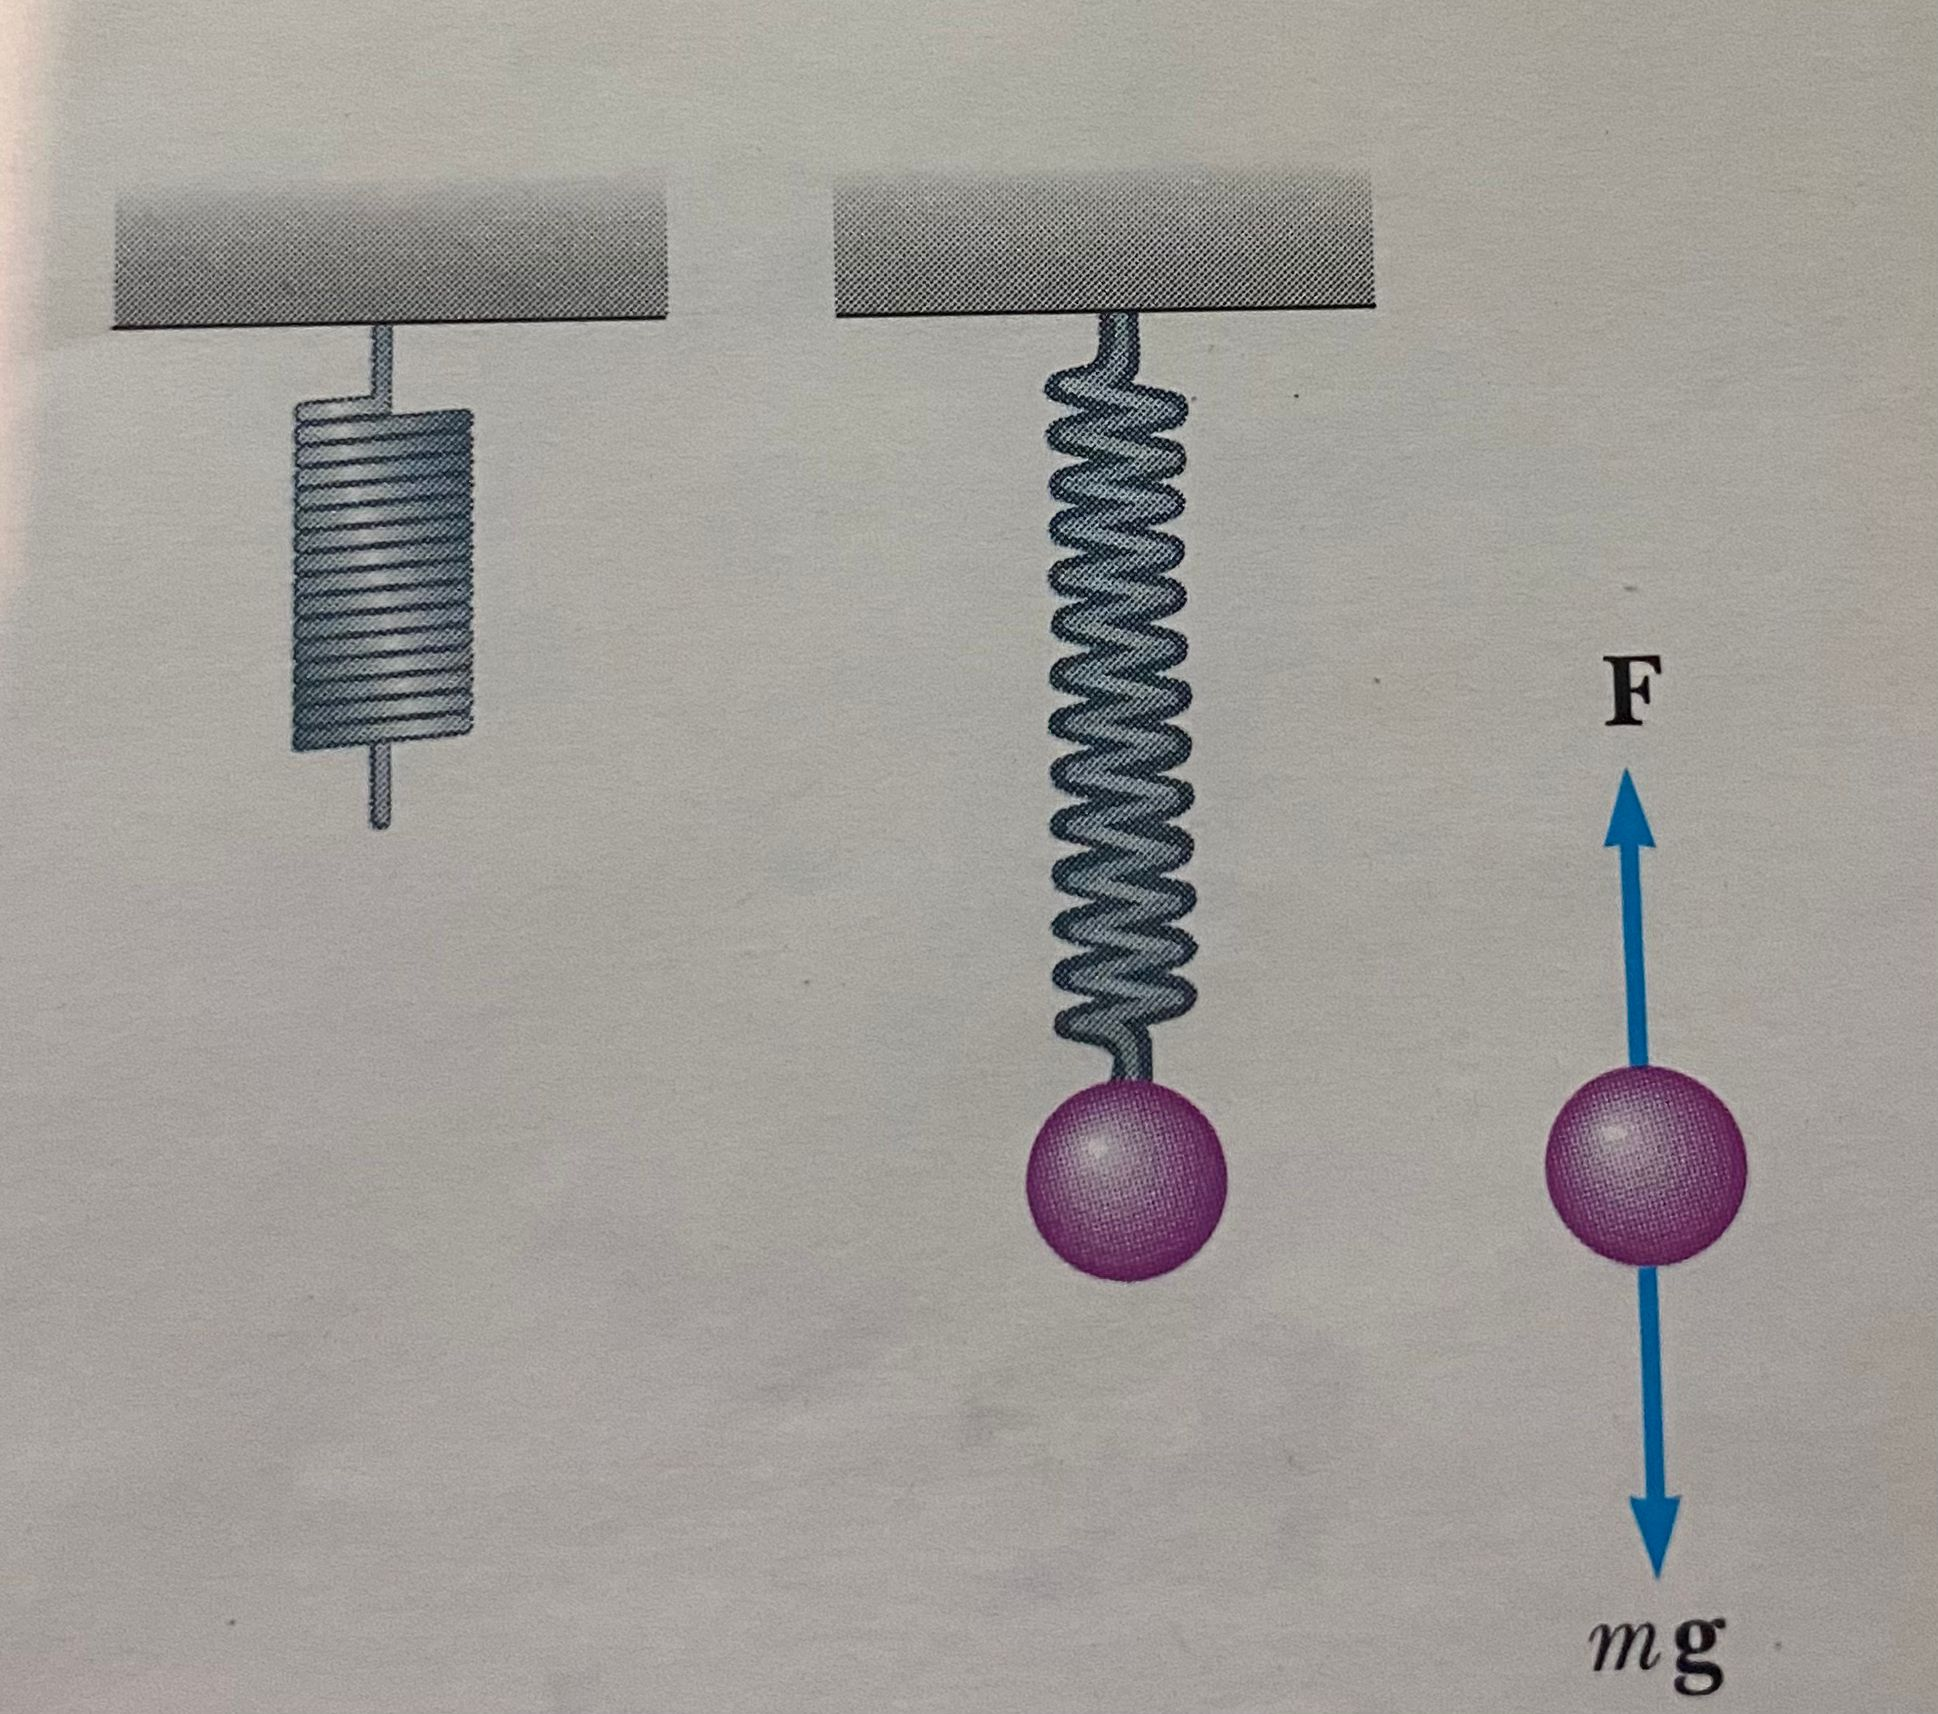
\includegraphics[width=\linewidth]{Dinamometro.jpeg}}
\end{minipage}%
\hfill
\begin{minipage}[t]{0.55\textwidth}
  \raggedright
La forza può essere misurata staticamente tramite un \textbf{dinamometro.} Una molla estesa esercita una forza di richiamo che entro certi limiti di allungamento è proporzionale all'allungamento stesso. Appendendo un corpo di massa m la forza F sviluppata dalla molla in condizioni di equilibrio eguaglia la forza esercitata dalla terra, che attira il corpo (F=mg). 
  \end{minipage}
  \newpage
  \subsection{Leggi di Newton}
La formulazione quantitativa del legame tra la forza e lo stato del moto è data dalla \textbf{legge di Newton (seconda)}:
\begin{equation}
    \vec{F} = m\vec{a} = m \frac{d\vec{v}}{dt}=m \frac{d^2\vec{r}}{dt^2}
\end{equation}
esprime la \textbf{legge fondamentale della dinamica del punto}.
L'interazione del punto con l'ambiente circostante, espresso tramite la forza F, determina l'accelerazione del punto, ovvero la variazione della sua velocità nel tempo: m è la massa inerziale del punto. \\
Il termine \textbf{massa inerziale} è legato al fatto che la massa esprime l'inerzia del punto, cioè la sua resistenza a variare il proprio stato di moto, ossia a modificare la velocità. Fissata una determinata forza F, l'effetto dinamico è tanto maggiore quanto è minore la massa del punto. Se una certa forza F agisce separatamente su due punti materiali diversi, questi acquistano accelerazioni diverse:
\begin{equation}
    F=m_1a_1=m_2a_2 \ \ -> \  \ \frac{m_2}{m_1}=\frac{a_1}{a_2}
\end{equation}
Se una delle due masse è nota possiamo ottenere la massa dell'altra confrontando le rispettive accelerazioni. Si giustifica così anche il nome \textbf{punto materiale}: per descrivere il comportamento dinamico del punto occorre conoscere la sua massa. In assenza di interazione con l'esterno la forza è nulla e quindi $\vec{a}=0,\vec{v}=costante$. Grazie alla (5.2.1) capiamo che dalle caratteristiche della forza si deducono quelle del moto. Seguendo Newton, noi chiamiamo forza ciò che causa una variazione dello stato di moto di un corpo. La legge di Newton è valida solo se il moto è studiato in una particolare classe di sistemi di riferimento, i cosiddetti \textbf{sistemi di riferimento inerziali}. Inoltre la legge di Newton è applicabile solo se la velocità dei punti considerati è molto minore della velocità della luce, $c=3 \cdot10^8 ms^{-1}$.
\subsubsection{Terza legge di Newton}
\begin{minipage}[t]{0.4\textwidth}
  \raisebox{-\height}{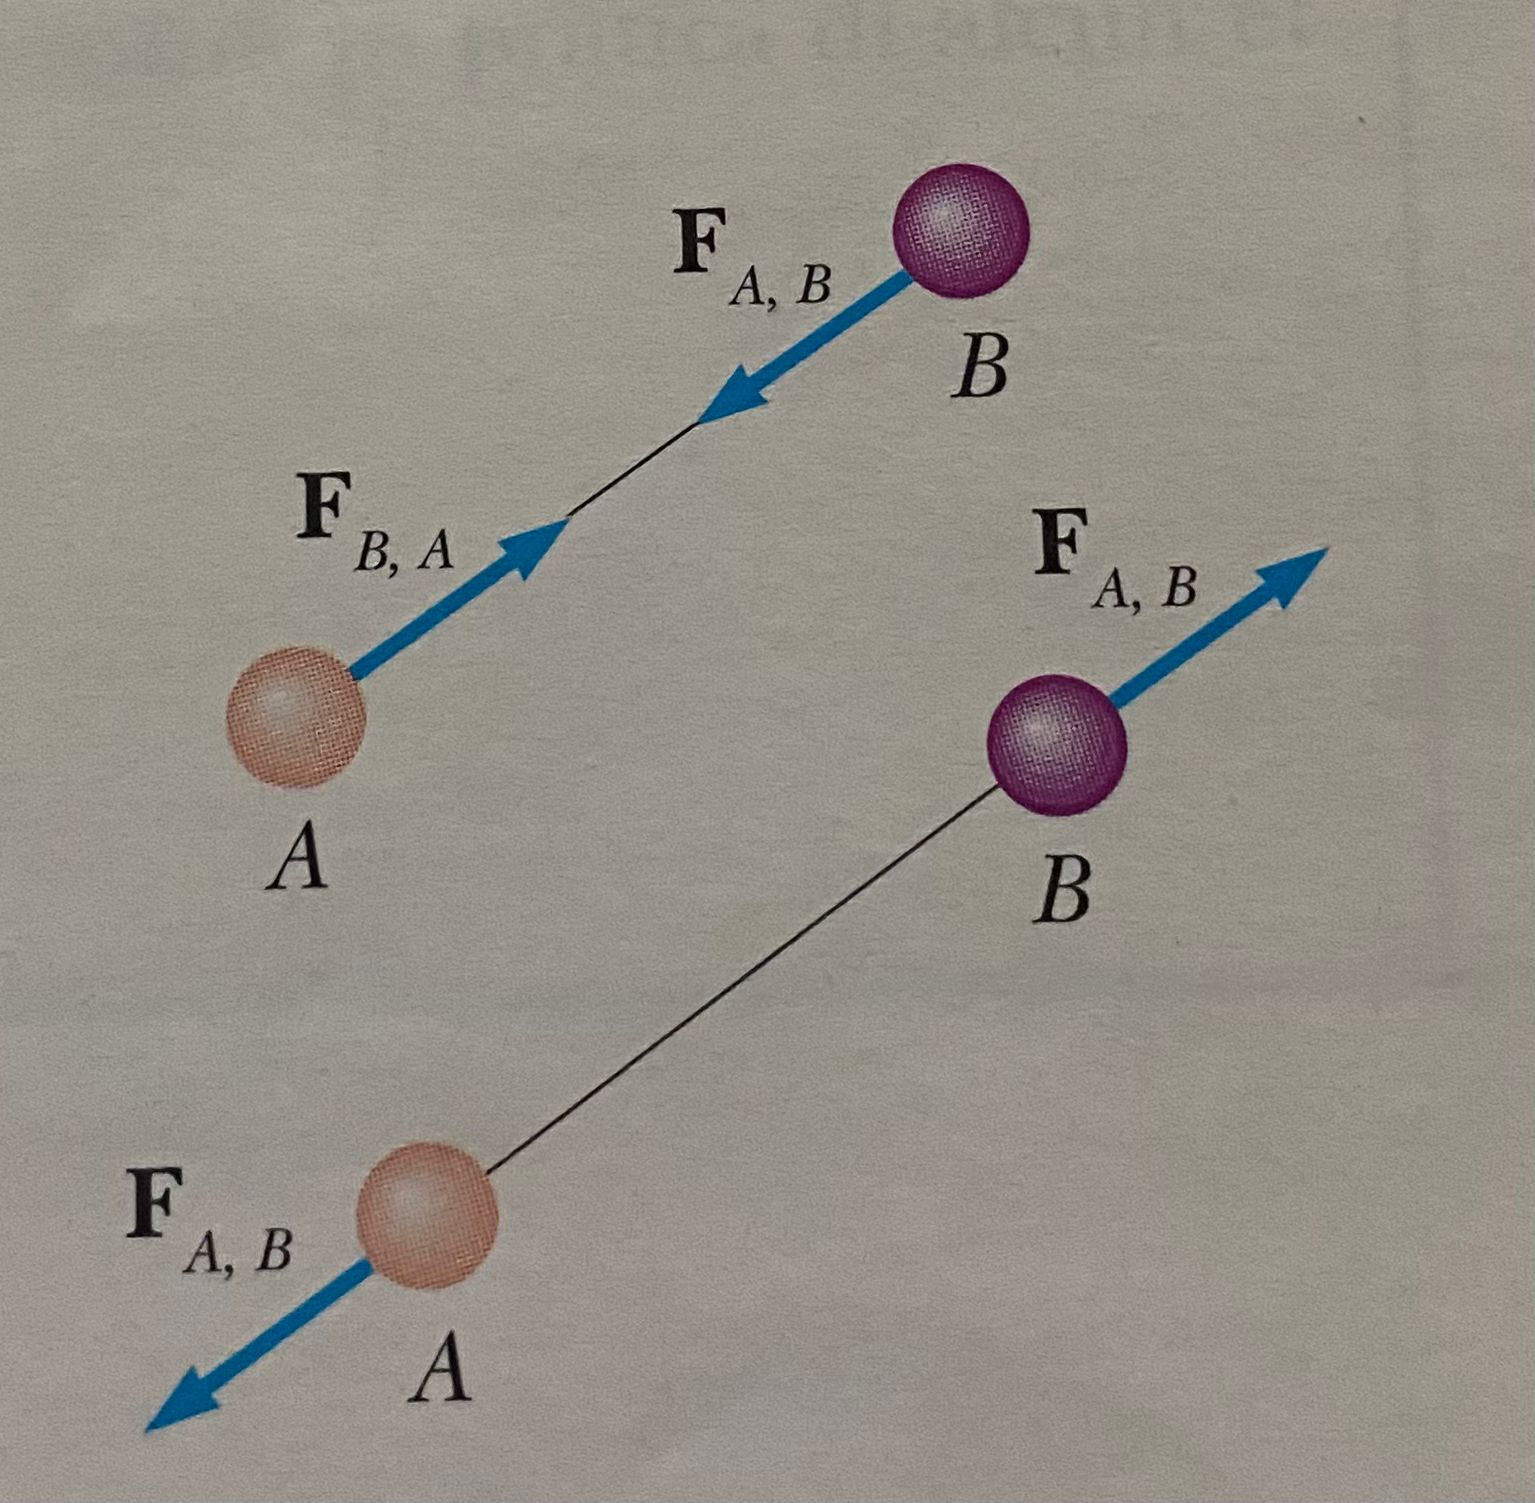
\includegraphics[width=\linewidth]{TerzaLeggeDiNewton.jpeg}}
\end{minipage}%
\hfill
\begin{minipage}[t]{0.55\textwidth}
  \raggedright
Newton scoprì anche una proprietà generale delle forze, che si può enunciare in questa forma:
\begin{itemize}
    \item se un corpo A esercita una forza $\vec{F}_{A,B}$ su un corpo B, il corpo B reagisce esercitando una forza $\vec{F}_{B,A}$ sul corpo A.
    \item le due forze hanno la stessa direzione, lo stesso modulo e verso opposto, esse cioè sono uguali e contrarie:
    \begin{equation}
        \vec{F}_{A,B}=-\vec{F}_{B,A}
    \end{equation}
    \item le due forze hanno la stesa retta d'azione
\end{itemize}
Questa legge è anche detta \textbf{principio di azione e reazione delle forze.}
  \end{minipage}
  \subsection{Quantità di moto. Impulso}
  Si definisce \textbf{quantità di moto} di un punto materiale il vettore:
  \begin{equation}
      \vec{p}= m\vec{v}
  \end{equation}
  se la massa è costante si può scrivere:
  \begin{equation}
      \vec{F}=\frac{d\vec{p}}{dt}
  \end{equation}
  Questa è la \textbf{forma più generale della seconda legge di Newton}. Lo stato dinamico del punto è individuato dalla quantità di moto, in cui compaiono la massa e la velocità. L'azione di una forza determina la variazione nel tempo della quantità di moto ovvero di qualcuna o di tutte queste quantità, massa, direzione, verso, modulo della velocità. Dalla (5.3.2) si ha $\vec{F}dt=d\vec{p}$: vediamo che l'azione di una forza durante un tempo dt provoca una variazione infinitesima della quantità di moto del punto. In termini finiti si ha:
  \begin{equation}
      \vec{J}=\int_{0}^t \vec{F}dt = \int_{p_0}^p d\vec{p}= \vec{p}-\vec{p}_0=\Delta \vec{p}
  \end{equation}
  Il termine vettoriale $\vec{J}$, integrale della forza nel tempo, è chiamato \textbf{impulso della forza} e la relazione sopra descritta viene anche detta \textbf{forma integrale della seconda legge di Newton} ed esprime il \textbf{teorema dell'impulso:}\\
  \begin{itemize}
      \item L'impulso di una forza applicata a un punto materiale provoca la variazione della quantità di moto;
      \item se la massa m è costante allora:
      \begin{equation}
          \vec{J}=m (\vec{v}-\vec{v_0})=m \Delta v
      \end{equation}
  \end{itemize}
\textbf{Valore medio $F_m$ della forza}:
\begin{equation}
    \vec{F}_m= \frac{\Delta \vec{p}}{t}
\end{equation}
Quando F è nulla, $\Delta \vec{p}=0$ e pertanto $\vec{p}=costante$; vale il \textbf{principio di conservazione della quantità di moto:}\\
In assenza di forze applicate la quantità di moto di un punto materiale rimane costante, ovvero si conserva.
\subsection{Risultante delle forze. Equilibrio. Reazioni vincolari}
Un'importante verifica di questa affermazione si ha quando su un punto materiale agiscono contemporaneamente più forze, si constata che il moto del punto ha luogo come se agisse una sola forza, la \textbf{risultante vettoriale delle forze} applicate al punto:
\begin{equation}
    \vec{R} = \sum_i \vec{F}_i
    \end{equation}
in effetti l'\textbf{accelerazione del punto} è pari alla somma vettoriale delle accelerazioni che il punto avrebbe se agisse ciascuna forza da sola:
\begin{equation}
    \vec{a}=\frac{\vec{R}}{m}=\sum_i\frac{\vec{F}_i}{m}=\sum_ia_i
\end{equation}
Questo fondamentale risultato sperimentale fa capire che in presenza di più forze ciascuna agisce indipendentemente dalle altre. Si parla a tale proposito di \textbf{indipendenza delle azioni simultanee}. In particolare \textbf{affermare che la forza agente su un punto è nulla non significa necessariamente che sul punto non agiscono forze, ma spesso indica che la somma delle forze agenti su di esso, cioè la risultante, è nulla.} Se $\vec{R}=0$ e il punto ha inizialmente velocità nulla, esso rimane in quiete: sono realizzate le condizioni di \textbf{equilibrio statico} del punto. Devono quindi essere nulle le componenti della risultante. In generale, dato un insieme di forze applicate ad un punto e aventi risultante $\vec{R}'$, l'\textbf{equilibrio statico} si ottiene applicando al punto una forza eguale ed opposta a $\vec{R}'$, così da realizzare appunto la condizione $\vec{R}=0$.
\subsubsection{Reazioni vincolari}
Se un corpo, soggetto all'azione di una forza o della risultante non nulla di un'insieme di forze, rimane fermo, dobbiamo dedurre da quanto detto sopra che l'azione della forza provoca una reazione dell'ambiente circostante, detta \textbf{reazione vincolare}, che si esprime tramite una forza, eguale e contraria alla forza o alla risultante delle forze agenti, applicata al corpo stesso in modo tale che esso rimanga in quiete. \textbf{In generale la reazione vincolare non è determinabile a priori, utilizzando una data formula, ma deve essere calcolata caso per caso dall'esame delle condizioni fisiche.}
\begin{align}
    & x_1(t)=v_0t - \frac{1}{2}at^2 \\
    & x_2(t)=x_0+\frac{1}{2}at^2 \\
    & v_0t - \frac{1}{2}at^2=x_0+\frac{1}{2}at^2 \\
    & x_{1,2}= \frac{v_0+-\sqrt{v_0^2-4ax_0}}{2a}
\end{align}
\subsection{Azione dinamica delle forze}
Nel caso più generale la forza F non è costante e il \textbf{moto} è \textbf{vario}, con accelerazione non costante. Se il \textbf{moto} è \textbf{rettilineo uniforme} (v=costante, a=0) si ha ovviamente F=0. Se il \textbf{moto} è \textbf{uniformemente accelerato} (a=costante) la forza agente è vettorialmente costante (quindi in direzione, verso e modulo). Abbiamo visto poi che nel \textbf{moto piano curvilineo} l'accelerazione presenta due componenti $a_T \ \ e \ \ a_N$. Pertanto:
\begin{equation}
    \vec{F} = m\vec{a}_T+m\vec{a}_N= m\frac{dv}{dt}\vec{u}_T+m\frac{v^2}{R}\vec{u}_N
\end{equation}
La risultante delle forze agenti sul punto materiale deve avere una componente ortogonale alla traiettoria, $\vec{F}_N$, per provocare la variazione di direzione della velocità. La componente tangenziale $\vec{F}_T$ della forza determina invece la variazione del modulo della velocità. $F_N$ si chiama \textbf{forza centripeta} ed è sempre diversa da zero in un moto curvilineo. La forza centripeta non è un tipo di forza.
\subsection{Forza Peso}
Sperimentalmente si osserva che in uno stesso luogo tutti i corpi qualunque sia la massa inerziale, assumono se lasciati liberi la stessa \textbf{accelerazione}, detta  \textbf{di gravita}. Tale accelerazione è conseguenza della forza di attrazione terrestre, cioè dell'interazione gravitazionale tra la terra e il corpo. Dalla formula della forza troviamo che se agisce solo la forza peso $\vec{P}$ abbiamo $\vec{P}=m\vec{a}=m\vec{g}$ visto che a=g. Pertanto \textbf{la forza peso risulta proporzionale alla massa} e si scrive sempre:
\begin{equation}
    \vec{P}=m\vec{g}
\end{equation}
Si tratta di una forza costante e in assenza di altre forze il moto ha una componente uniformemente accelerata nella direzione parallela a g. Se invece agiscono altre forze in generale si ha $a \neq g$. La proporzionalità tra forza peso e massa suggerisce che il confronto tra due masse possa essere effettuatoa confrontando le rispettive forze peso;è su questa idea che si basa il metodo di misura delle masse tramite la \textbf{bilancia}.
\subsubsection{La sensazione di peso}
Un corpo di massa m, poggiato su un pavimento e in equilibrio statico, esercita una forza sul pavimento e risente di una reazione N che in modulo vale mg. Questa reazione applicata sul nostro corpo ci da la sensazione di peso.
\begin{equation}
    \vec{N}+\vec{P}=m\vec{a} \ \ -> \ \ \vec{N}+m\vec{g}=m\vec{a} \ \ -> \  \ \vec{N}=m(\vec{a}-\vec{g})
\end{equation}
Abbiamo quattro casi, per esaminarli prendiamo come asse di riferimento un asse verticale z orientato verso l'alto, per cui $\vec{g}=-g\vec{u}_z$:
\begin{itemize}
    \item Quando $a>0$ vi è un'accelerazione verso l'alto, $N>mg$, ci si \textbf{sente più pesanti}.
    \item Quanto $a<0$ vi è un accelerazione verso il basso $N<mg$ e si ha una \textbf{sensazione di diminuzione di peso}
    \item Quando a=g N=0 e \textbf{non c'è sensazione di peso}
    \item L'ultimo caso è quello in cui $a<0$ ma maggiore in modulo di g e questo non ha senso.
\end{itemize}
\subsection{Forza di attrito radente}
Applichiamo ad un corpo appoggiato su un tavolo orizzontale, una forza $\vec{F}$ parallela al piano di appoggio. Si osserva sperimentalmente che il corpo non entra in movimento per effetto di F fino a che il modulo di F non supera il valore $\mu_sN_s$, dove $\mu_s$ è il \textbf{coefficiente di attrito statico} e N, che è il modulo della componente normale al piano di appoggio della reazione vincolare. Abbiamo dunque:
\begin{equation}
    condizione \ \ di \ \ quiete \ \ F<=\mu_sN
\end{equation}
\begin{equation}
    condizione \ \ di \ \ moto \ \ F>\mu_sN
\end{equation}
\begin{minipage}[t]{0.4\textwidth}
  \raisebox{-\height}{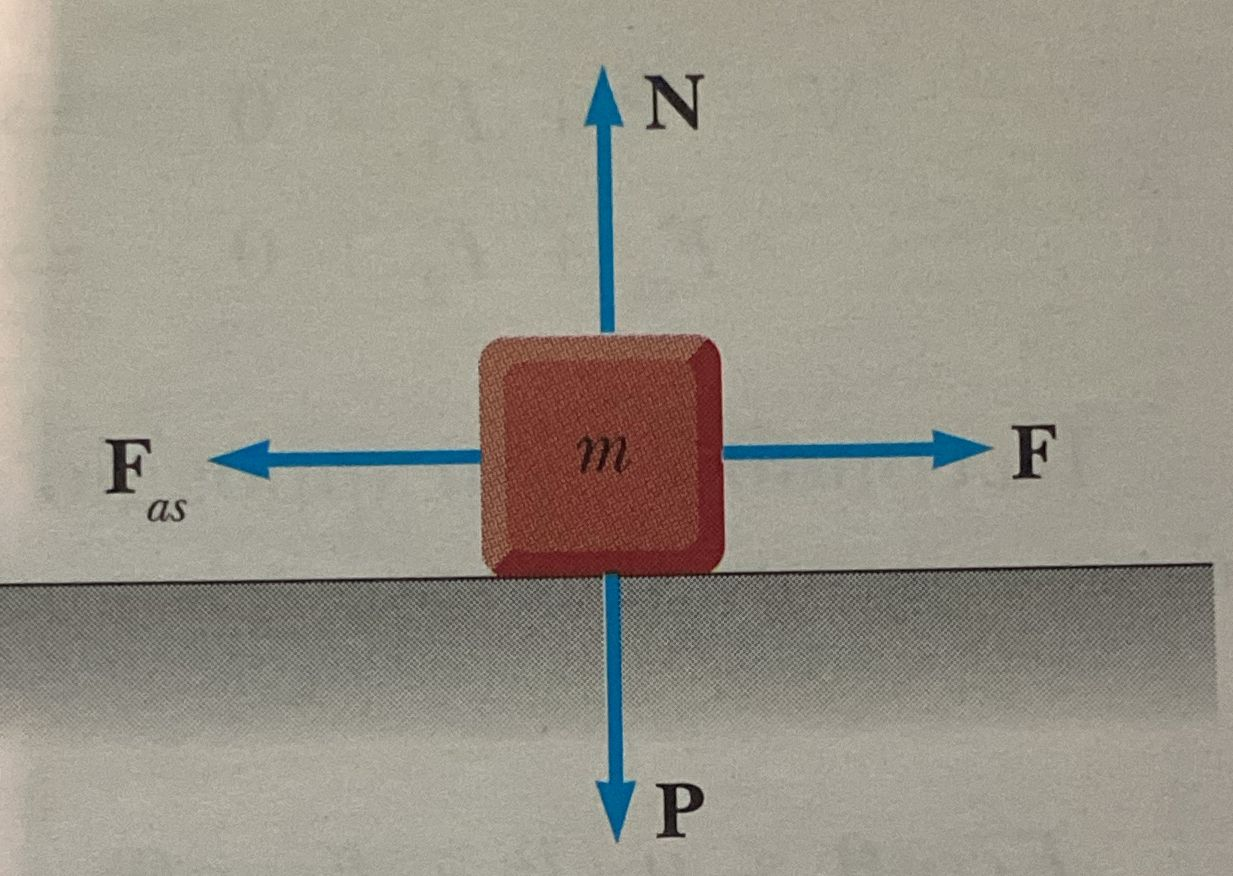
\includegraphics[width=\linewidth]{attritoStatico.jpeg}}
\end{minipage}%
\hfill
\begin{minipage}[t]{0.55\textwidth}
  \raggedright
In condizioni di quiete è realizzato l'equilibrio statico:
\begin{equation}
    \vec{R} + \vec{F}+\vec{P}=0
\end{equation}
dove R è la reazione vincolare del piano e P la forza peso del corpo. Dette N e $F_{as}$ le componenti verticale e orizzontale di R, in modulo:
\begin{equation}
    N=mg \ \ , \ \ F_{as}=F
\end{equation}
Il vincolo è in grado di sviluppare una \textbf{forza}, detta \textbf{di attrito radente statico}, eguale e contraria a F.  
  \end{minipage}
  Cio avviene fino a che F non supera il valore $\mu_sN$: la forza di attrito radente statico non ha pertanto un valore prefissato, ma varia con il valore della forza F applicata, da zero fino al massimo $\mu_sN$. Quando F supera $\mu_sN$ il corpo entra in movimento lungo il piano e si osserva che si oppone al moto la \textbf{forza di attrito radente dinamico} $F_{ad}=\mu_dN$ dove $\mu_d$ rappresenta il \textbf{coefficiente di attrito dinamico}; risulta sempre $\mu_d<\mu_s$. L'equazione del moto è pertanto
  \begin{equation}
      F-\mu_dN=ma
  \end{equation}
  Vettorialmente:
  \begin{equation}
      \vec{F}_{ad}=-\mu_dN\vec{u}_v
  \end{equation}
  Abbiamo detto che le forze di attrito radente hanno origine dalle \textbf{forze di coesione} tra due materiali; il valore del coefficiente di attrito dipende dallo stato delle superficie a contatto e dalla loro composizione chimica. 
  \newpage
  \subsection{Piano Inclinato}
  \begin{figure}[H] % Usa 'H' per forzare la posizione qui
    \centering % Centra l'immagine
    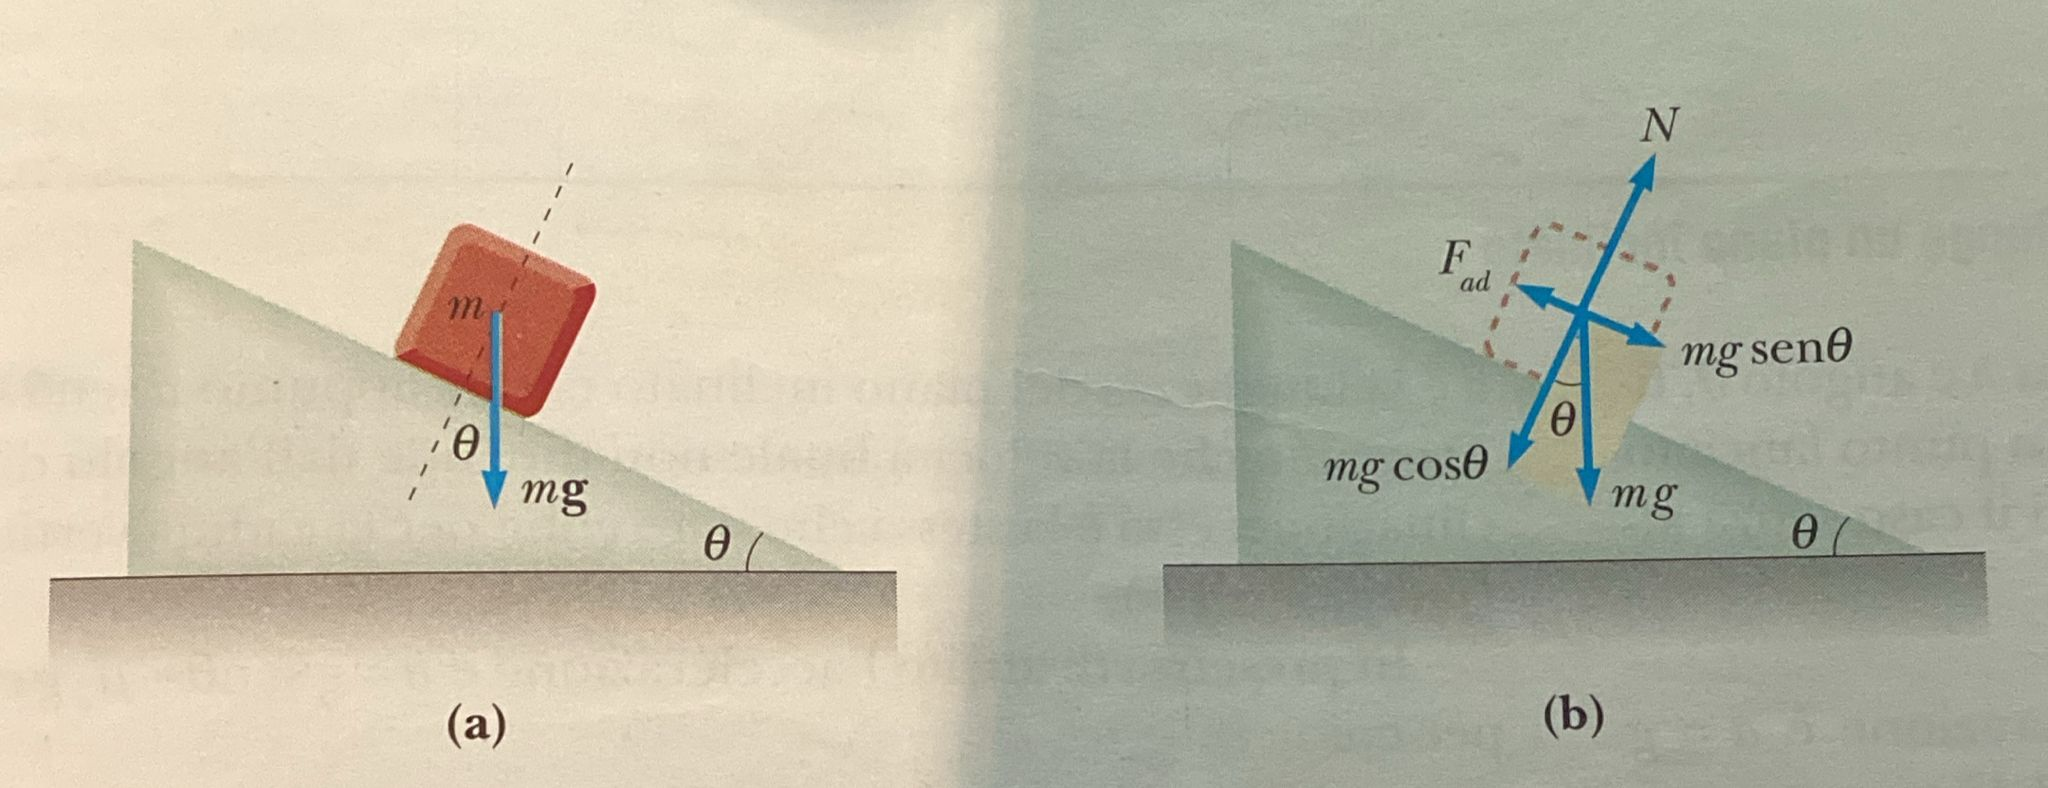
\includegraphics[width=8cm, height=4cm]{PianoInclinato.jpeg} % Percorso dell'immagine
    \caption{Traiettoria parabolica di un punto} % Didascalia per l'immagine
    \label{fig:immagine} % Etichetta per riferimento
\end{figure}
\noindent
Consideriamo un corpo assimilabile ad un punto materiale di massa m, che possa muoversi sotto l'azione del suo peso e di eventuali altre forze, compresa la forza di attrito radente, su una superficie piana inclinata di un angolo $\theta$ rispetto ad un piano orizzontale detto \textbf{piano inclinato}. Se agisce solo la forza peso P, in assenza perciò di attrito tra corpo e piano inclinato, si ha secondo la legge di Newton:
\begin{equation}
    \vec{P}+\vec{R}=m\vec{a}
\end{equation}
dove R è la reazione vincolare del piano di appoggio che ha un'unica componente normale al piano stesso, \textbf{vincolo liscio}. Scomponendo lungo le direzioni ortogonale e parallela al piano inclinato si ottiene:
\begin{equation}
    mgcos\theta-N=0 \ , \ mgsen\theta=ma
\end{equation}
dato che il corpo è vincolato a muoversi lungo il piano inclinato. Quindi $N=mgcos \theta$ e $a=gsen\theta<g$: il corpo scende con \textbf{moto uniformemente accelerato} e l'accelerazione è minore di quella di gravità. La \textbf{condizione per l'equilibrio statico} di un corpo poggiato su un piano inclinato scabro è:
\begin{equation}
    tg\theta<=\mu_s
\end{equation}
Vale l'equazione:
\begin{equation}
    a= (sen\theta-\mu_dcos\theta)g
\end{equation}
Dovendo essere il termine tra parentesi positivo, si ha per il coefficiente di attrito dinamico $\mu_d<tg\theta$; in particolare, se $\mu_d=tg\theta$ a=0: il moto è uniforme e si tratta di un esempio di equilibrio dinamico. Riassumendo, se il corpo è fermo sul piano inclinato esso resta fermo per tutti gli angoli di inclinazione compresi tra zero e $\theta_s$ tale che $tg\theta_s=\mu_s$; per $\theta>\theta_s$ il corpo non può restare fermo e scende lungo il piano inclinato. Se invece il corpo all'istante iniziale sta scendendo lungo il piano con velocità $v_0$, se $tg \theta<\mu_d$, si muove di moto uniformemente accelerato se $tg\theta>\mu_d$ e prosegue con velocità $v_0$ se $tg\theta=\mu_d$.
\subsection{Forza Elastica}
Si definisce \textbf{forza elastica} una forza di direzione costante, con verso rivolto sempre ad un punto O, chiamato centro, e con modulo proporzionale alla distanza da O. Se assumiamo come asse x la direzione della forza e come origine il centro, possiamo scrivere:
\begin{equation}
    \vec{F}=-kx\vec{u}_x
\end{equation}
Dove k è una costante positiva, detta \textbf{costante elastica}, e $u_x$ è il versore dell'asse x. Il moto risultante per effetto di una forza elastica è rettilineo, qualora la velocità iniziale sia nulla o diretta come $u_x$. L'accelerazione vale:
\begin{equation}
    a=\frac{F}{m}=\frac{-k}{m}x=-\omega^2x
\end{equation}
Il moto è armonico semplice con pulsazione $\omega$ e periodo T determinati dal rapporto tra la costante elastica e la massa del punto materiale a cui è applicata la forza elastica:
\begin{equation}
    \omega=\frac{k}{m} \ , \ T= \frac{2\pi}{\omega} = 2\pi \sqrt{\frac{m}{k}}
\end{equation}
\begin{minipage}[t]{0.4\textwidth}
  \raisebox{-\height}{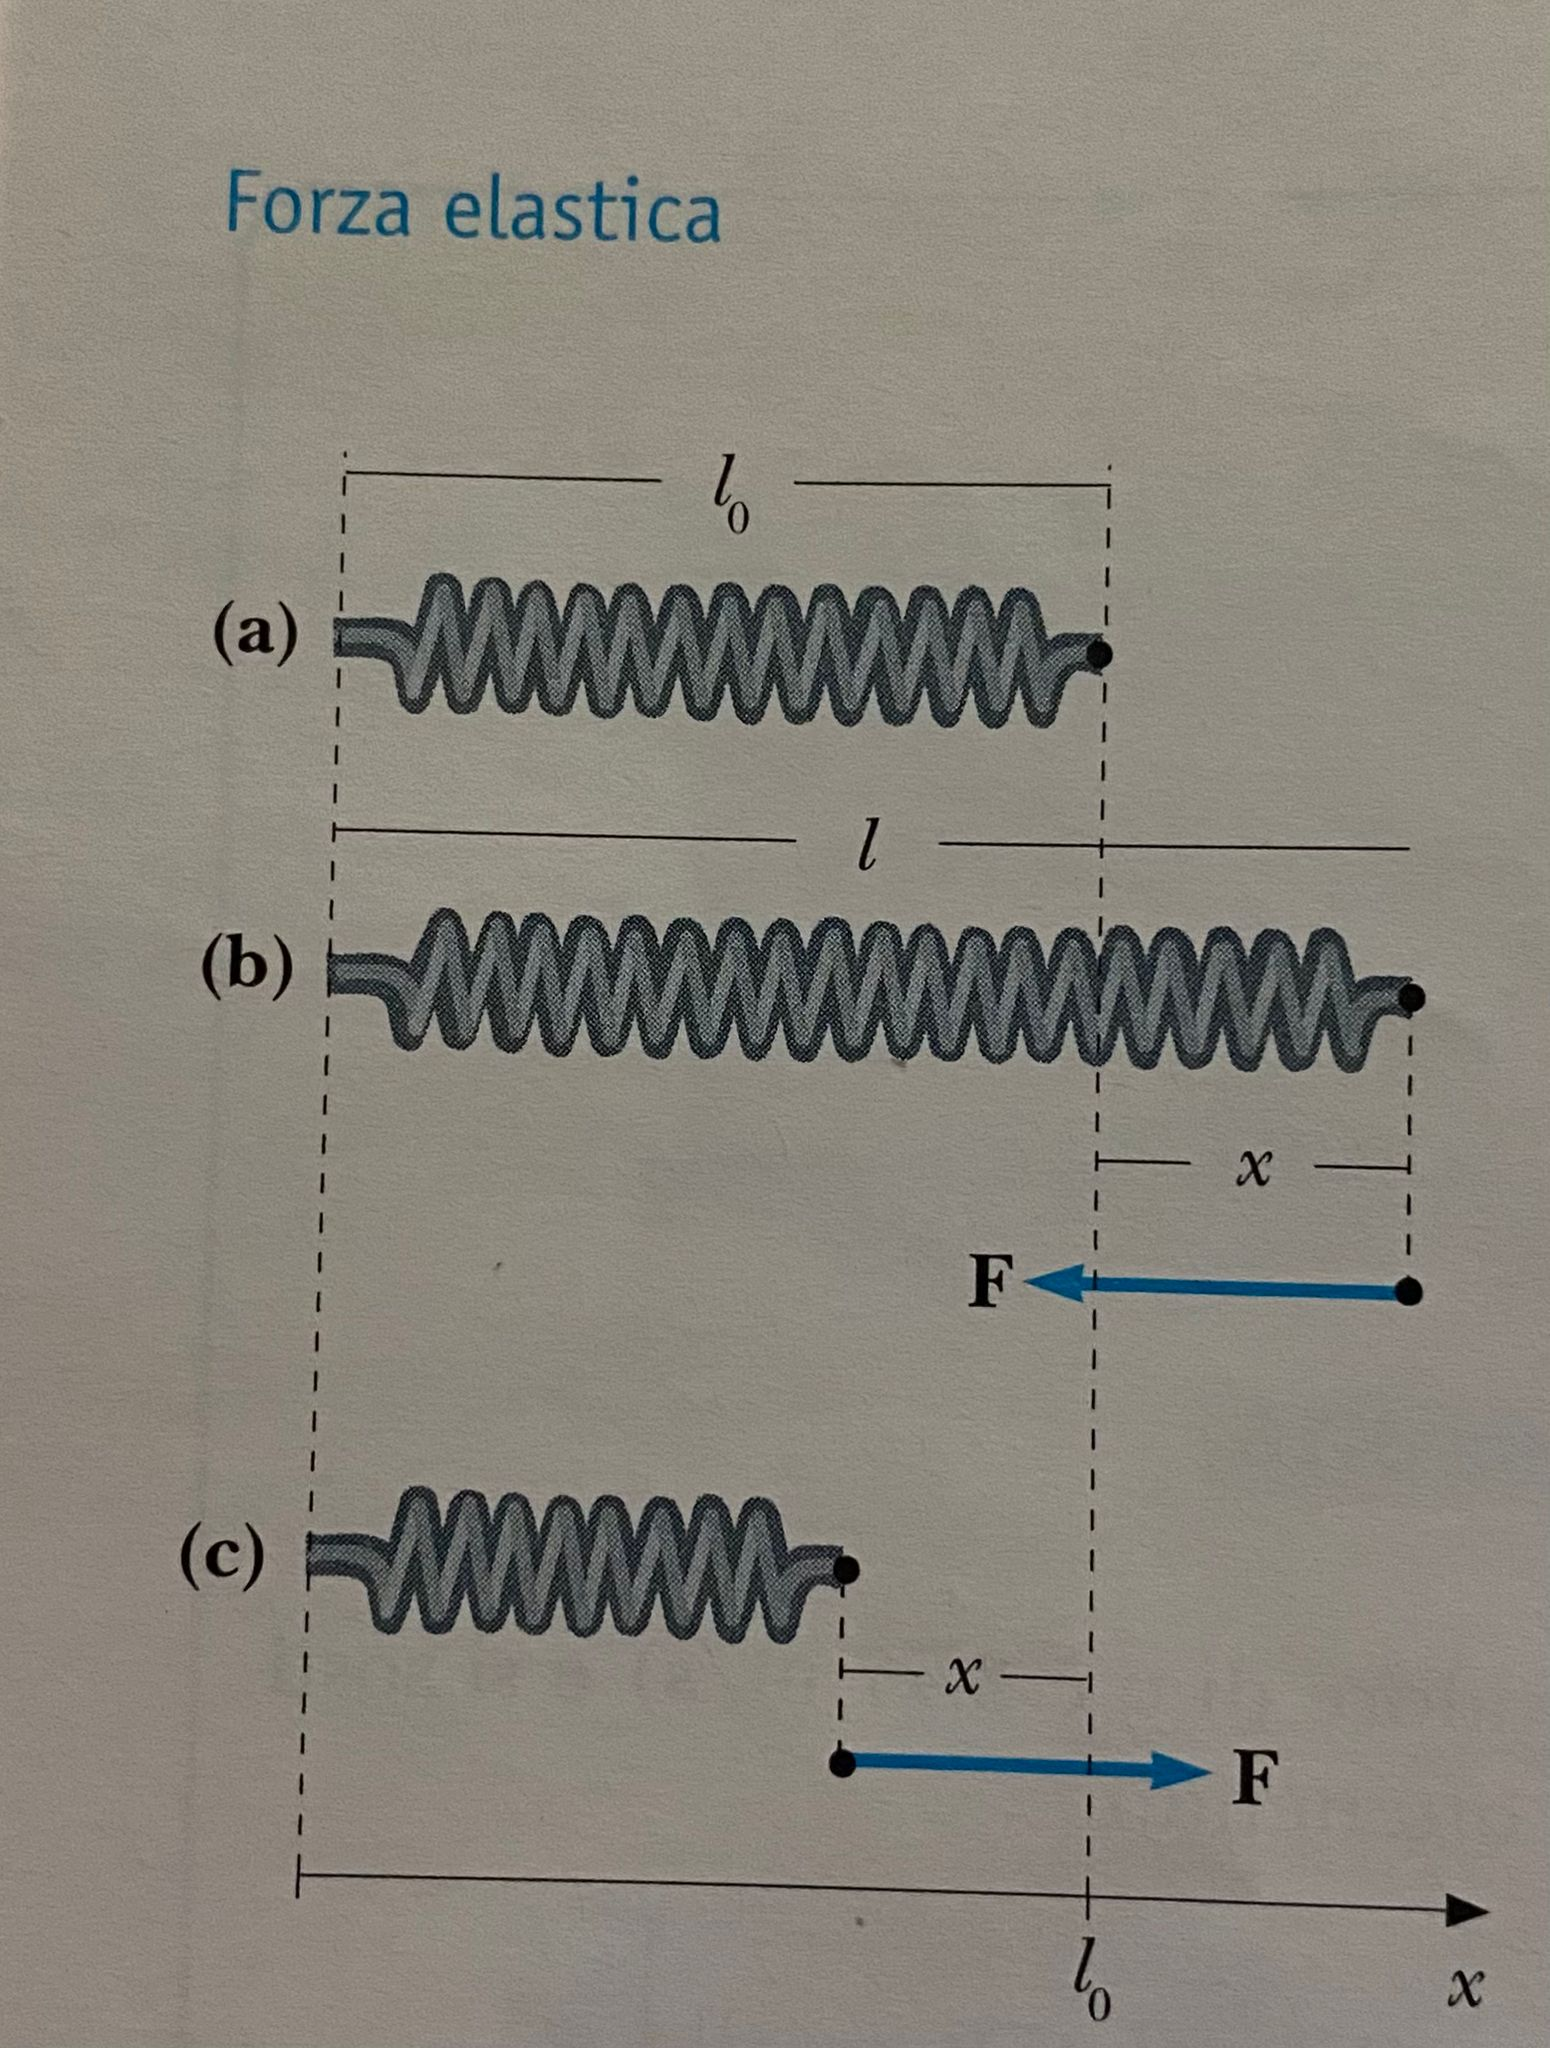
\includegraphics[width=\linewidth]{ForzaElastica.jpeg}}
\end{minipage}%
\hfill
\begin{minipage}[t]{0.55\textwidth}
  \raggedright
Una forza elastica viene praticamente applicata tramite una molla; questa presenta in genere una lunghezza a riposo, cioè quando non si trova in condizioni di compressione o di estensione, di valore finito $l_0$, figura a. Se la molla viene estesa, figura b, assumendo una lunghezza $l>l_0$, essa sviluppa una forza F che tende a riportarla alla condizione di riposo:
\begin{equation}
    F=-k(l-l_0)=-kx
\end{equation}
Se invece la molla viene compressa alla lunghezza $l<l_0$, figura c, la forza ha la stessa espressione, con $x<0$, ma opposta. Il modulo di questa \textbf{forza di richiamo} è proporzionale alla deformazione fino a che non si supera il limite di elasticità della molla. Se vogliamo mantenere la molla deformata con una determinata lunghezza l dobbiamo applicare a una molla una forza eguale ed opposta alla forza esercitata dalla molla. Legge oraria e velocita:
\begin{equation}
    x=x_0cos\omega t \ , \ v=-\omega x_0 sen \omega t
\end{equation}
  \end{minipage}
  \subsection{Forza di attrito viscoso}
   La \textbf{forza di attrito viscoso} è una forza che si oppone al moto ed è proporzionale alla velocità del corpo soggetto a tale forza:
   \begin{equation}
       \vec{F}=-b\vec{v}
   \end{equation}
   L'accelerazione risulta $\vec{a}=-b\vec{v}/m$. In presenza di una forza di attrito viscoso non si può realizzare una condizione di equilibrio statico poichè se v=0 la forza si annulla. Forze di attrito viscoso sono esercitate, in certe condizioni, su un corpo che si muove in un fluido (liquido o gas).
   \begin{equation}
       v(t)=\frac{g}{k}(1-e^{-kt})
   \end{equation}
   Dove 1/k è la costante di tempo $\tau$.
   \subsection{Forze Centripete}
   Supponiamo che la risultante R delle forze agenti su un punto materiale presenti una componente $F_N$ ortogonale alla traiettoria, che risulta pertanto curvilinea. $F_N$ determina l'\textbf{accelerazione centripeta} secondo la relazione $F_N=ma_N=mv^2/r$ essendo r il raggio di curvatura della traiettoria. In generale R ha anche una componente tangente alla traiettoria, $F_T$, responsabile della variazione del modulo della velocità. Se $F_T=0$ il moto lungo la traiettoria è uniforme e l'unica accelerazione è $a_N$. Forze centripete sono generalmente prodotte da rotaie, pneumatici, fili che collegano il corpo ad un punto fisso ovvero vincoli che consentono di incurvare la traiettoria oppure da azioni a distanza come quelle gravitazionali.
\subsection{Pendolo Semplice}
   \begin{minipage}[t]{0.4\textwidth}
  \raisebox{-\height}{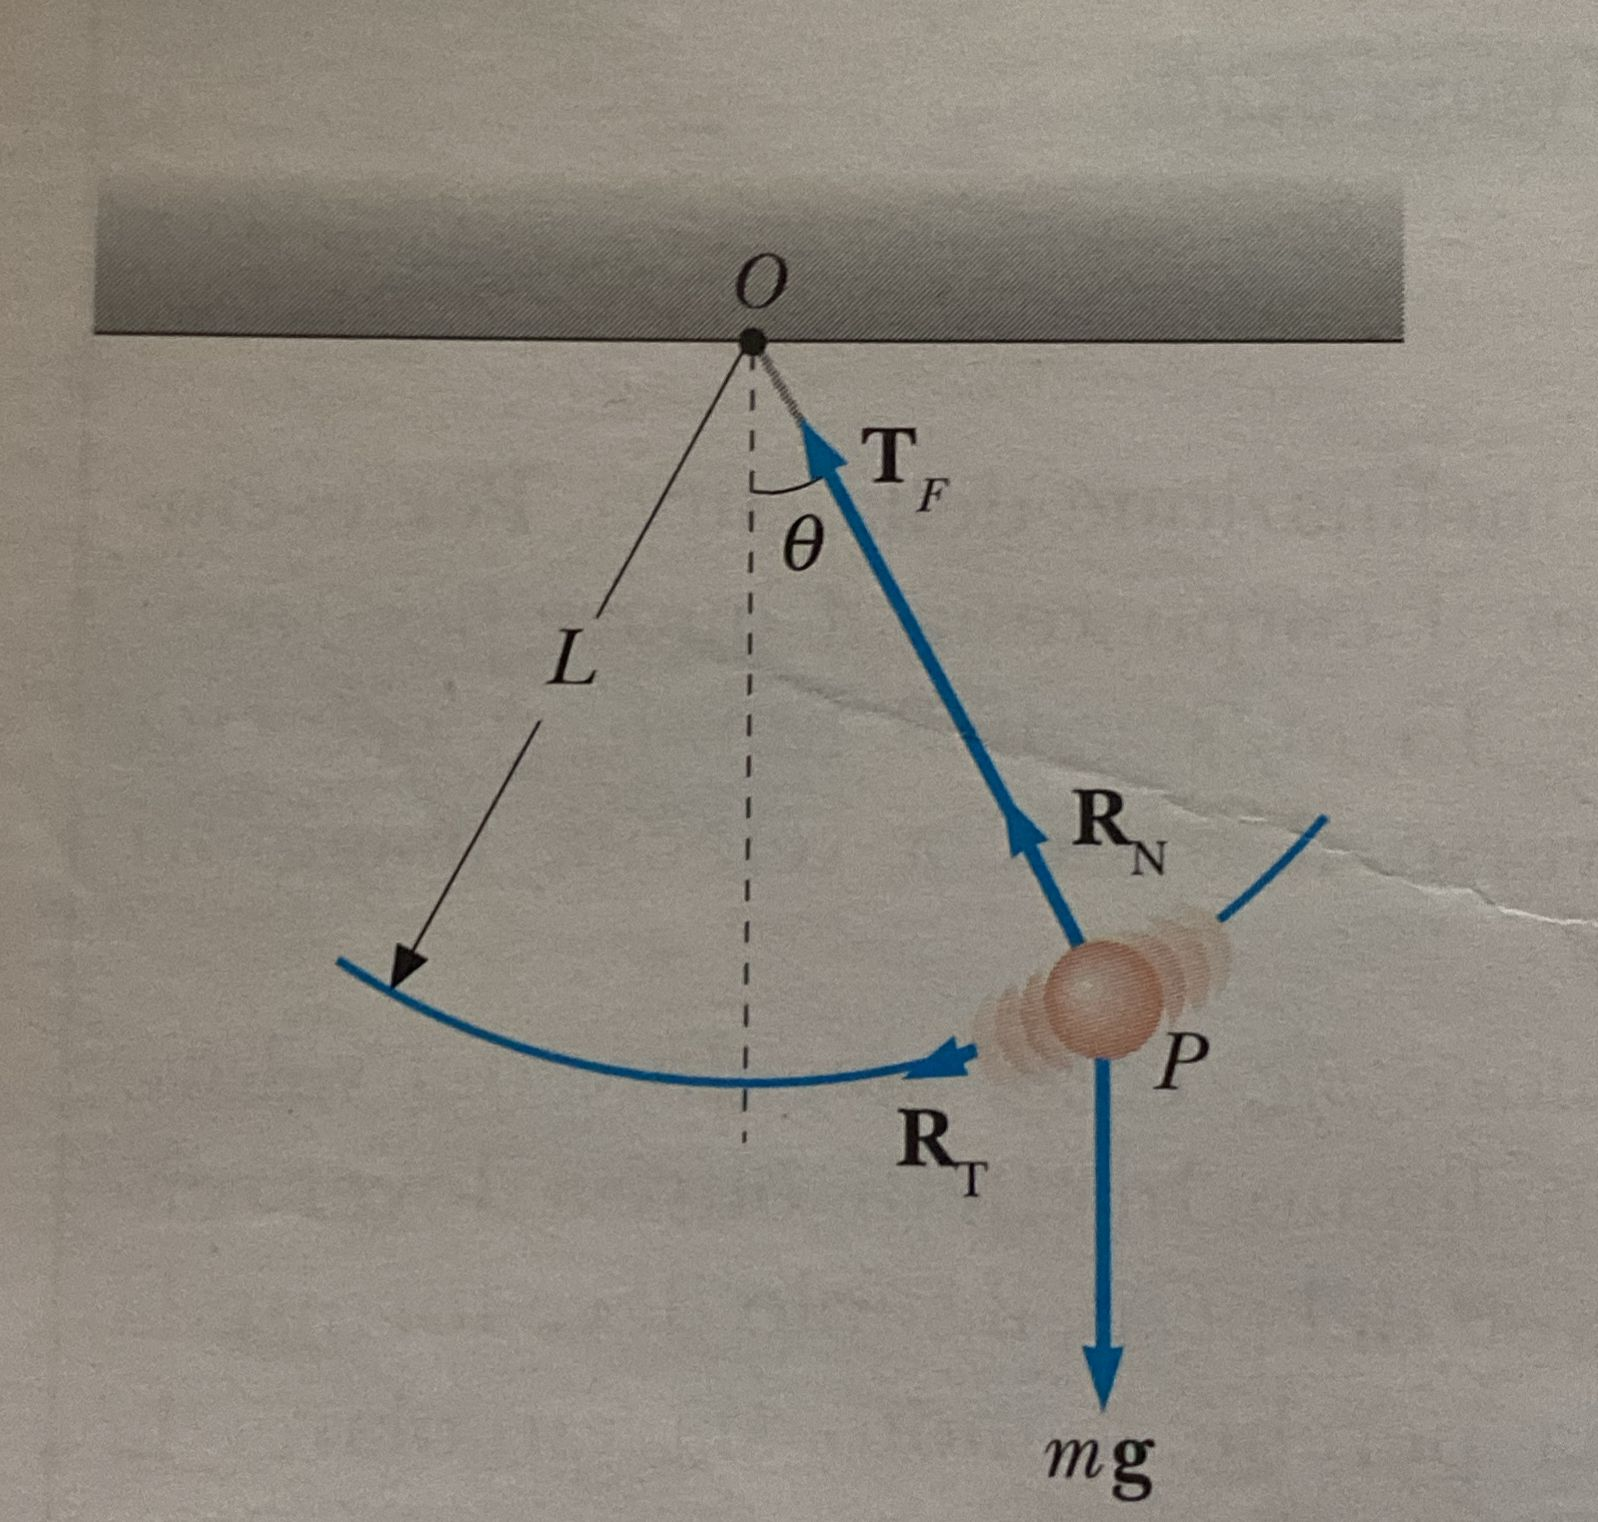
\includegraphics[width=\linewidth]{PendoloSemplice.jpeg}}
\end{minipage}%
\hfill
\begin{minipage}[t]{0.55\textwidth}
  \raggedright
Il \textbf{Pendolo semplice} è costituito da un punto materiale appeso tramite un filo inestensibile e di massa trascurabile. La posizione di equilibrio statico è quella verticale, con il punto fermo ed il filo teso; la forza esercitata dal filo vale in modulo $T_F=mg$. Se spostiamo il punto dalla verticale esso inizia a oscillare attorno a questa, lungo un arco di circonferenza di raggio L, pari alla lunghezza del filo, in un piano verticale. Le forze agenti sul punto P sono il peso mg e la tensione del filo $\vec{T}_F$ per cui il moto è regolato da $m\vec{g}+\vec{T}_F=ma$. Per quanto riguarda le componenti lungo la traiettoria, abbiamo che $\vec{R}_T$ è una \textbf{forza di richiamo} che tende a riportare il punto sulla verticale, anche se non è di direzione costante come nel caso delle forze elastiche. Il moto del pendolo è oscillatorio quando l'ampiezza delle oscillazioni è piccola cosi che $sen\theta\approx\theta$. Il \textbf{periodo del moto} T è dato da:
\begin{equation}
    T=\frac{2\pi}{\omega}=2\pi\sqrt{\frac{L}{g}}
\end{equation}
ed è indipendente dall'ampiezza. La \textbf{legge oraria dello spostamento} lungo l'arco di circonferenza è dato da (dove $\theta_0$ è l'ampiezza dell'oscillazione e $\phi$ è la fase iniziale):
\begin{equation}
    s=L\theta=L\theta_0sen(\omega t + \phi)
\end{equation}
\end{minipage}
  Mentre la velocità angolare e la velocità lineare hanno le espressioni:
  \begin{align}
     &  \omega=\frac{d\theta}{dt}=\omega\theta_0cos(\omega t + \phi) \\
     & v= \frac{ds}{dt}=L\frac{d\theta}{dt}=L\omega\theta_0cos(\omega t+\phi)
  \end{align}
    La velocità è massima quando il punto passa per la verticale ($\theta=0$) e nulla agli estremi delle oscillazioni ($\theta=\theta_0$) dove il verso del moto si inverte. Quando l'ampiezza delle oscillazioni non è piccola il moto è ancora periodico, ma non armonico. Risolto il problema del moto, e quindi note $\theta(t)$ e v(t), possiamo ritornare all'equazione del moto proiettata sulla normale alla traiettoria e calcolare la \textbf{tensione del filo} che sostiene il punto:
    \begin{equation}
        T_F=m[gcos\theta(t)+\frac{v^2(t)}{L}]
    \end{equation}
    La tensione è massima nella posizione verticale, dove sia $cos\theta(t)$ che v(t) assumono i valori massimi, ed è minima nei punti di inversione.
\subsection{Tensione dei fili}
   \begin{minipage}[t]{0.4\textwidth}
  \raisebox{-\height}{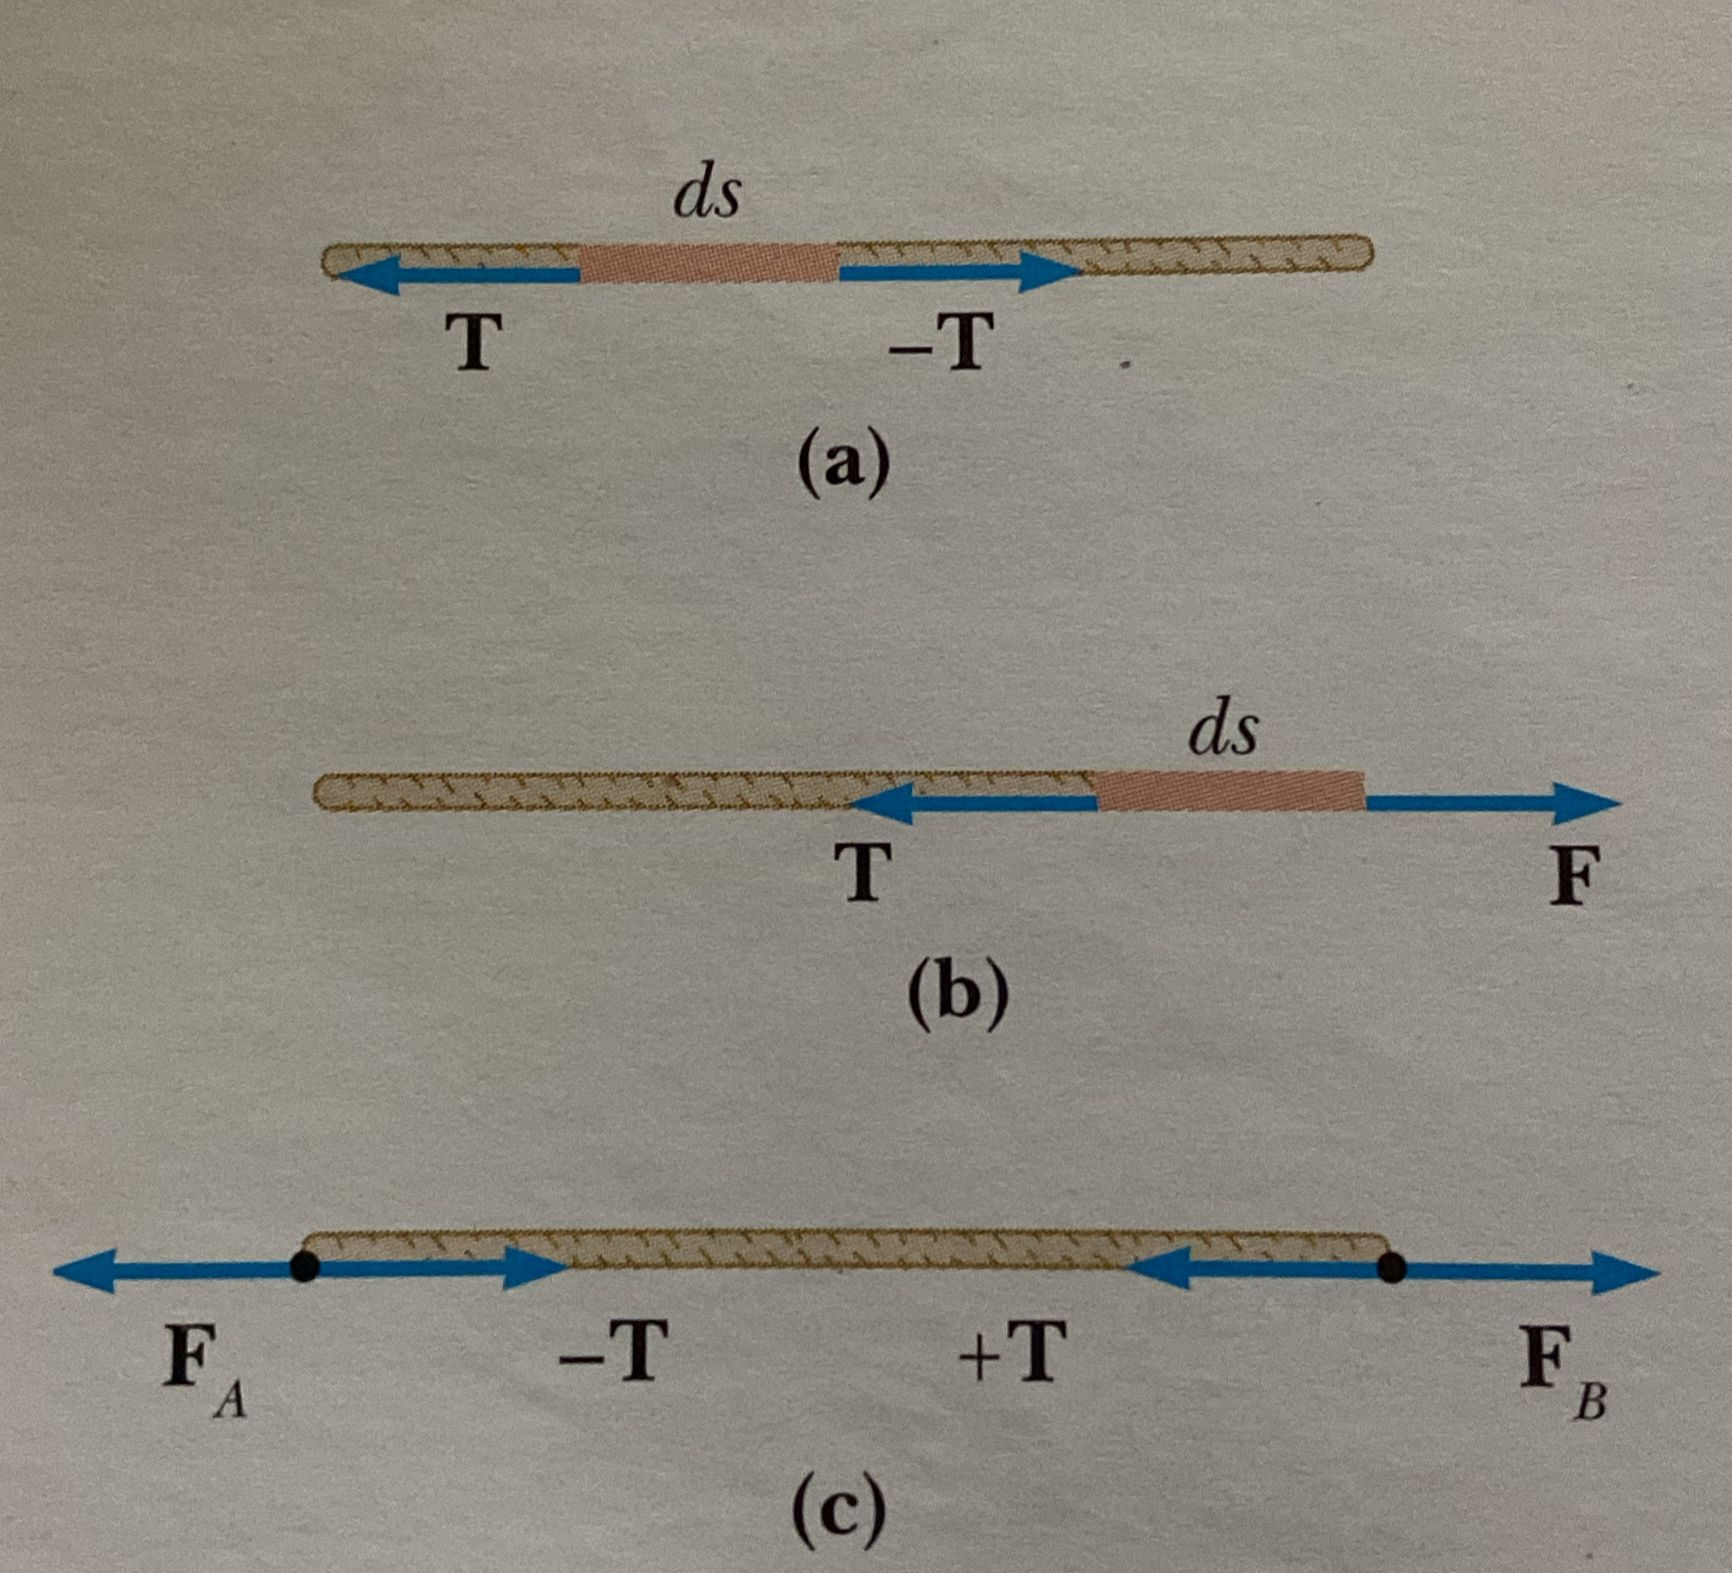
\includegraphics[width=\linewidth]{TensioneDeiFili.jpeg}}
\end{minipage}%
\hfill
\begin{minipage}[t]{0.55\textwidth}
  \raggedright
Nel pendolo semplice il filo di sostegno serve per applicare una certa forza al punto in movimento: il filo risulta teso e la forza, con direzione lungo il filo teso, che questo esercita sul punto viene chiamata \textbf{tensione del filo}. Per chiarire il concetto di tensione consideriamo un \textbf{filo teso in quiete} e prendiamo in esame un elemento infinitesimo ds di esso. Tale elemento è tirato dalle due parti restanti di filo e l'equilibrio statico richiede che le due forze agenti sull'elemento di filo siano eguali in modulo e direzione e di verso opposto. In particolare ad un estremo, $\vec{T}=\vec{-F}$. Per il filo nel suo insieme si ha la situazione della figura c e deve essere in modulo $F_A=F_B=T$: per tendere il filo si applicano le forze F e -F e la tensione, in modulo è eguale al modulo di F. 

\end{minipage}
\vspace{30pt}
Se consideriamo un \textbf{filo in movimento}, l'ipotesi che il filo abbia massa trascurabile fa si che ma=0 per il filo: di conseguenza il valore della tensione durante il moto è lo stesso in qualunque punto del filo, come nel caso statico. Quindi il filo esercita agli estremi la tensione $\vec{T}$, il cui valore dipende dalle forze applicate, e che deve essere pensata come la reazione del filo alla forza che lo tende. Per un filo reale la tensione non può superare un valore massimo $T_{max}$ oltre il quale il filo si spezza.
\section{Dinamica del punto: lavoro, energia, momenti}
\subsection{Lavoro. Potenza. Energia Cinetica}
 \begin{minipage}[t]{0.4\textwidth}
  \raisebox{-\height}{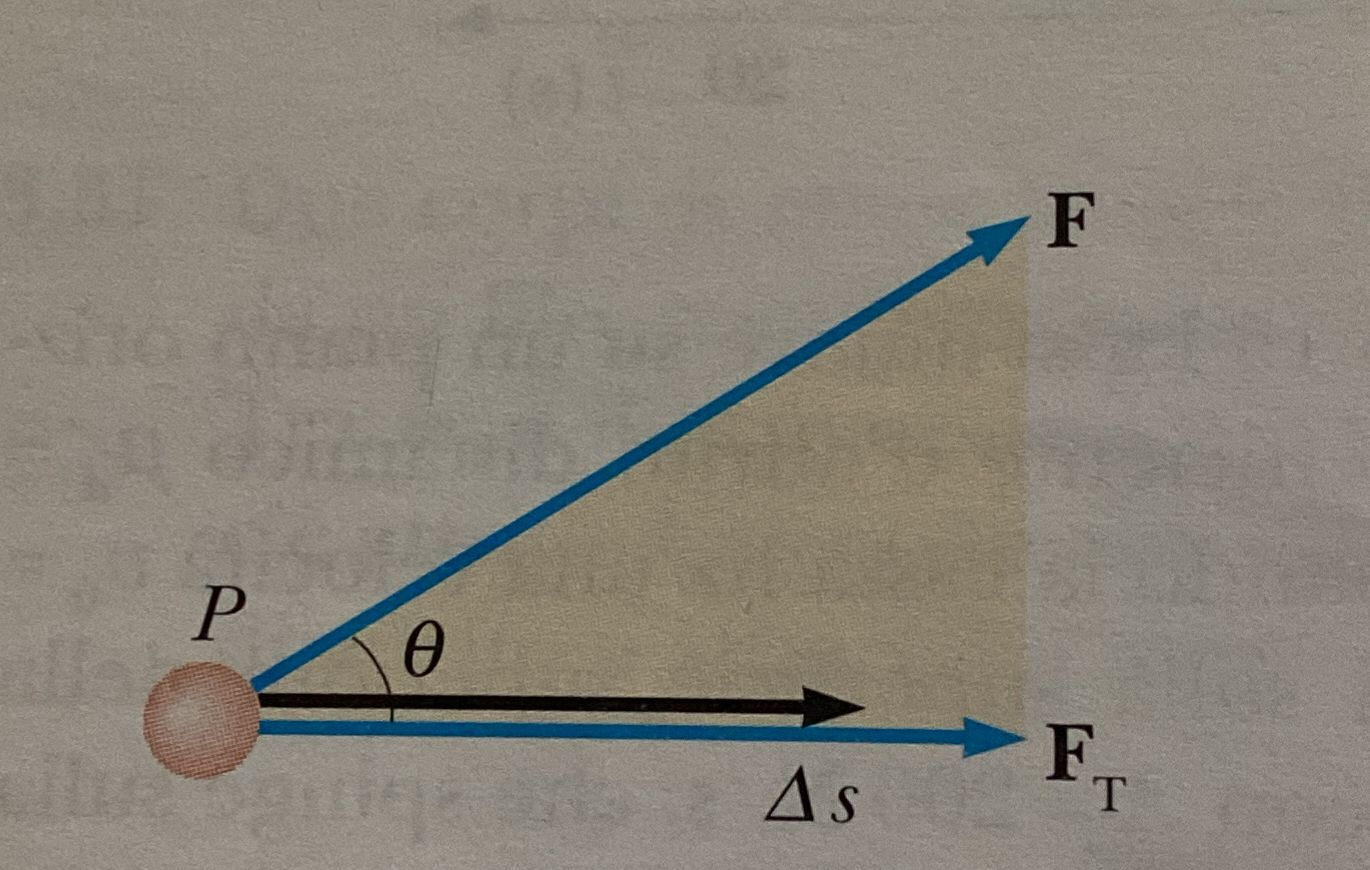
\includegraphics[width=\linewidth]{Lavoro.jpeg}}
\end{minipage}%
\hfill
\begin{minipage}[t]{0.55\textwidth}
  \raggedright
Consideriamo, un punto matriale P soggetto a una forza F che subisca, per azione di questa forza, uno spostamento $\Delta s$. Il \textbf{lavoro W compiuto dalla forza per lo spostamento $\Delta s$} è definito come il prodotto scalare della forza per lo spostamento:
\begin{equation}
    W = \vec{F} \cdot \vec{\Delta s}= f \Delta scos\theta= F_T\Delta s
\end{equation}
Dove $\theta$ è l'angolo tra F e $\Delta s$ e $F_T=Fcos\theta$ è la proiezione della forza lungo la direzione dello spostamento. La figura mostra che il lavoro dipende oltre che dal modulo della forza e dello spostamento, anche dall'angolo $\theta$, che determina il valore di $F_T$. Si possono presentare tre casi: F forma con $\Delta s$ un angolo minore di $\pi/2$, per cui l'accelerazione tangente è concorde con la velocità e la fa aumentare: W risulta positivo e viene chiamato \textbf{lavoro motore}. Oppure F forma con $\Delta s$ un angolo maggiore di $\pi/2$, per cui il punto viene frenato e W risulta negativo, \textbf{lavoro resistente}. Infine se F è ortogonale alla traiettoria, $\theta=\pi/2$ e il \textbf{lavoro è nullo}: in questo caso F ha un \textbf{azione} puramente \textbf{centripeta} e non fa variare il modulo della velocità.
\begin{equation}
    W=\int_A^B F \cdot ds= \int_A^B F cos\theta \ ds=\int_A^B F_T ds
\end{equation}
Dunque \textbf{il lavoro è l'integrale di linea della forza lungo la traiettoria}. 
\end{minipage}
Inoltre \textbf{il lavoro è pari alla somma dei lavori delle singole forze agenti, ciascuno dei quali può essere positivo, negativo o nullo.} Esempi di lavoro nullo: Un esempio di moto con risultante nulla delle forze è il moto rettilineo uniforme in presenza di attrito radente: occorre applicare una forza eguale e contraria alla forza di attrito e quindi fornire un lavoro motore eguale ed opposto al lavoro resistente dell'attrito. Invece un moto con risultante delle forze sempre ortogonale alla traiettoria è il moto curvilineo uniforme; se poi c'è attrito, oltre alla forza normale deve essere presente una forza tangente, che svolge un lavoro motore, per bilanciare l'effetto dell'attrito.
\subsubsection{Potenza}
La \textbf{potenza} corrisponde al lavoro per unità di tempo:
\begin{equation}
    \mathcal{P}=\frac{dW}{dt}= \vec{F} \cdot \frac{d\vec{r}}{dt}= \vec{F} \cdot \vec{v}= F_Tv
\end{equation}
Questa è la \textbf{potenza istantanea}, in generale variabile durante il moto, e caratterizza la rapidità di erogazione del lavoro. La \textbf{potenza media} è il rapporto W/t, cioè il lavoro totale diviso per il tempo durante cui il lavoro è stato svolto.
\subsubsection{Energia cinetica}
Riprendiamo la relazione relativa al lavoro infinitesimo associato ad uno spostamento ds:
\begin{equation}
    dW=F_Tds=ma_Tds=m\frac{dv}{dt}ds=m\frac{ds}{dt}dv=mvdv
\end{equation}
Per un percorso finito dalla posizione A a quella B abbiamo:
\begin{equation}
    W=\int_A^Bmvdv=\frac{1}{2}mv^2_B-\frac{1}{2}mv^2_A=E_{k,B} - E_{k,A} = \Delta E_k
\end{equation}
Dove la quantità $E_k=\frac{1}{2}mv^2$ prende il nome di \textbf{energia cinetica} del punto (Chat GPT: L'energia cinetica è l'energia che un corpo possiede a causa del suo movimento) e il simbolo $\Delta$ indica la differenza tra il valore nella posizione finale e quello nella posizione iniziale. Pertanto l'equazione soprascritta nota come \textbf{teorema dell'energia cinetica} afferma che: \\\\
Qualunque sia la forza che agisce nello spostamento di un punto mateirale dalla posizione A alla posizione B il lavoro fatto dalla forza è uguale alla variazione dell'energia cinetica del punto materiale stesso.\\\\
Se $W>0$, l'energia cinetica finale è maggiore di quella iniziale mentre se $W<0$ l'energia cinetica finale è minore di quella iniziale. Infine, se $W=0$, l'energia cinetica resta costante. Ciò si verifica, per esempio, nel moto circolare uniforme: il lavoro della forza centripeta, unica forza agente, è nullo e quindi la velocità rimane costante in modulo. Se misuriamo la velocità iniziale e finale, possiamo dedurre il lavoro compiuto dalle forze agenti. Se non c'è spostamento non può esserci lavoro, qualunque sia la forza applicata. Se riprendiamo le definizioni di energia cinetica e di quantità di moto:
\begin{equation}
    E_K=\frac{1}{2}mv^2 \ \ , \ \ \vec{p}=m\vec{v}
\end{equation}
vediamo che tra energia cinetica e modulo della quantità di moto sussistono le relazioni:
\begin{equation}
    E_K=\frac{p^2}{2m} \ \ , \ \ p=\sqrt{2mE_K}
\end{equation}
Tutte le leggi con cui vengono definite le varie forme di energia contengono sempre la variazione di energia e pertanto tali quantità possono essere definite a meno di una costante. Il lavoro è la manifestazione dell'azione di una forza ed è quindi conseguenza dell'interazione con l'ambiente circostante. Si parla pertanto di \textbf{lavoro scambiato} e non si dice mai che un sistema possiede lavoro. Si parla invece di \textbf{energia posseduta} dal sistema, che viene modificata dall'interazione con l'ambiente esterno.
\subsection{Lavoro della forza peso}
 \begin{minipage}[t]{0.4\textwidth}
  \raisebox{-\height}{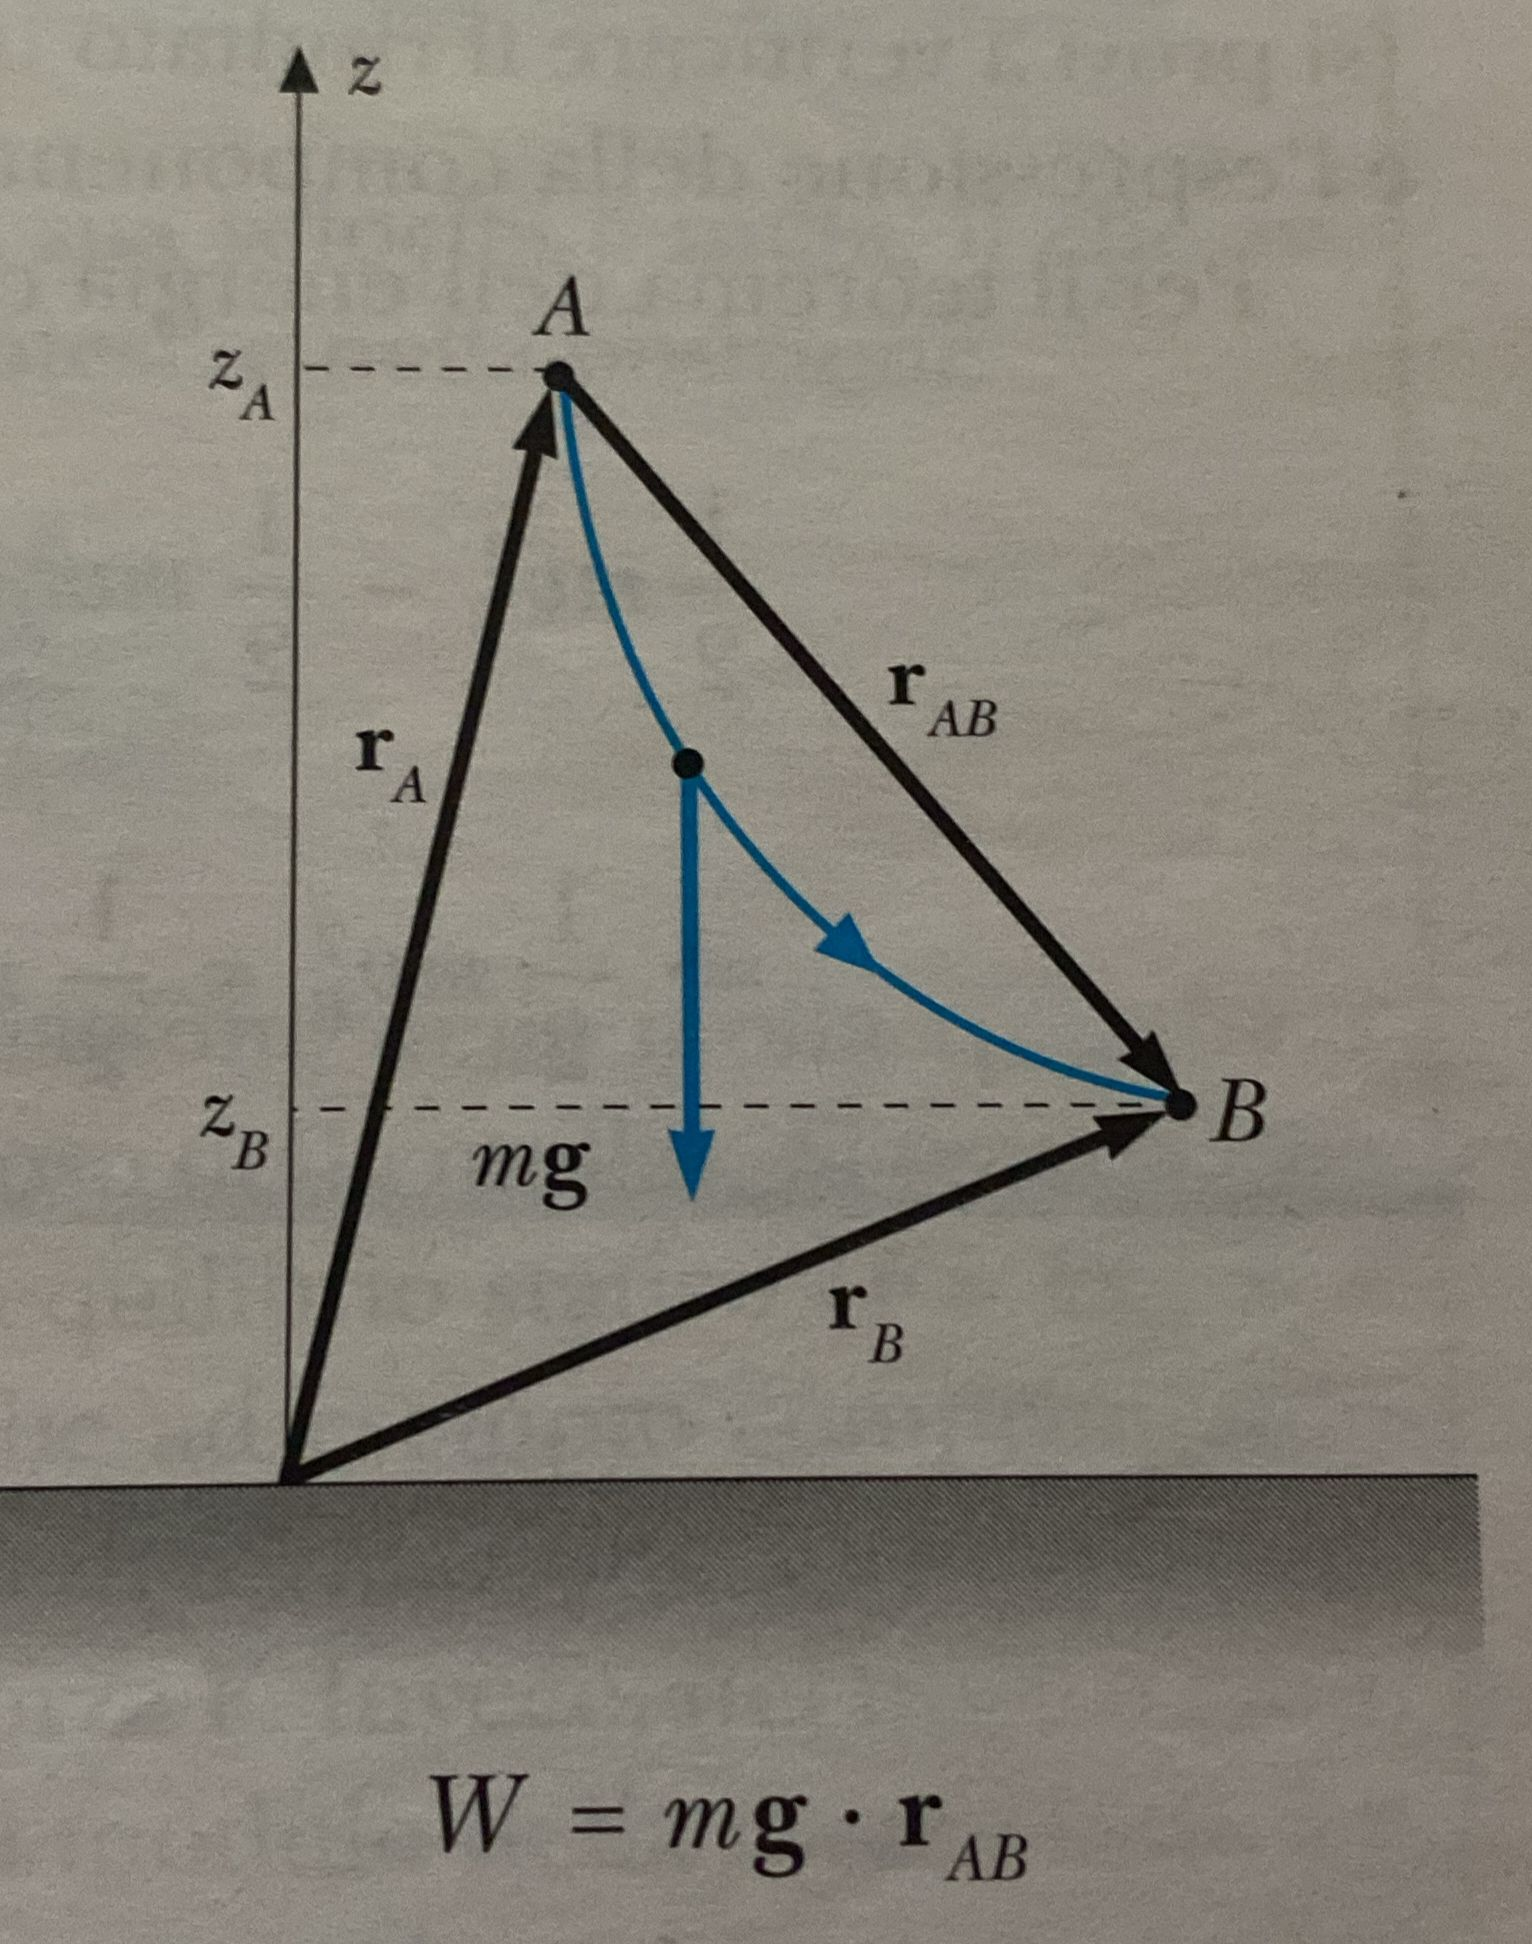
\includegraphics[width=\linewidth, keepaspectratio]{LavoroForzaPeso.jpeg}}
\end{minipage}%
\hfill
\begin{minipage}[t]{0.55\textwidth}
  \raggedright
Calcoliamo il \textbf{lavoro della forza peso mg} per uno spostamento generico dalla posizione A a quella B. L'asse z è orientato dal suolo verso l'alto ed ha quindi verso opposto a g.
\begin{equation}
    W=\int_A^B \vec{F} \cdot d\vec{s}=\vec{F} \cdot \int_A^B d\vec{s} = m\vec{g} \cdot\vec{r}_{AB}
\end{equation}
Poichè il peso ha una sola componente diversa da zero, quella secondo l'asse z che vale -mg, e la componente di $\vec{r}_{AB}$ lungo l'asse z è $z_B-z_A$, il prodotto scalare si scrive semplicemente $(mg)_z(r_{AB})_z=-mg(z_B-z_A)$ e pertanto il lavoro della forza peso vale:
\begin{equation}
    W= -(mgz_B - mgz_A) = -(E_{p,B} - E_{p,A}) = -\Delta E_p
\end{equation}
Dove con $E=mgz$ indichiamo l'\textbf{energia potenziale della forza peso}, dunque:
Il lavoro della forza peso è uguale all'opposto della variazione dell'energia potenziale della forza peso durante lo spostamento da A a B e pertanto non dipende dalla particolare traiettoria che collega A e B.
\end{minipage}
\newpage
 \begin{minipage}[t]{0.4\textwidth}
  \raisebox{-\height}{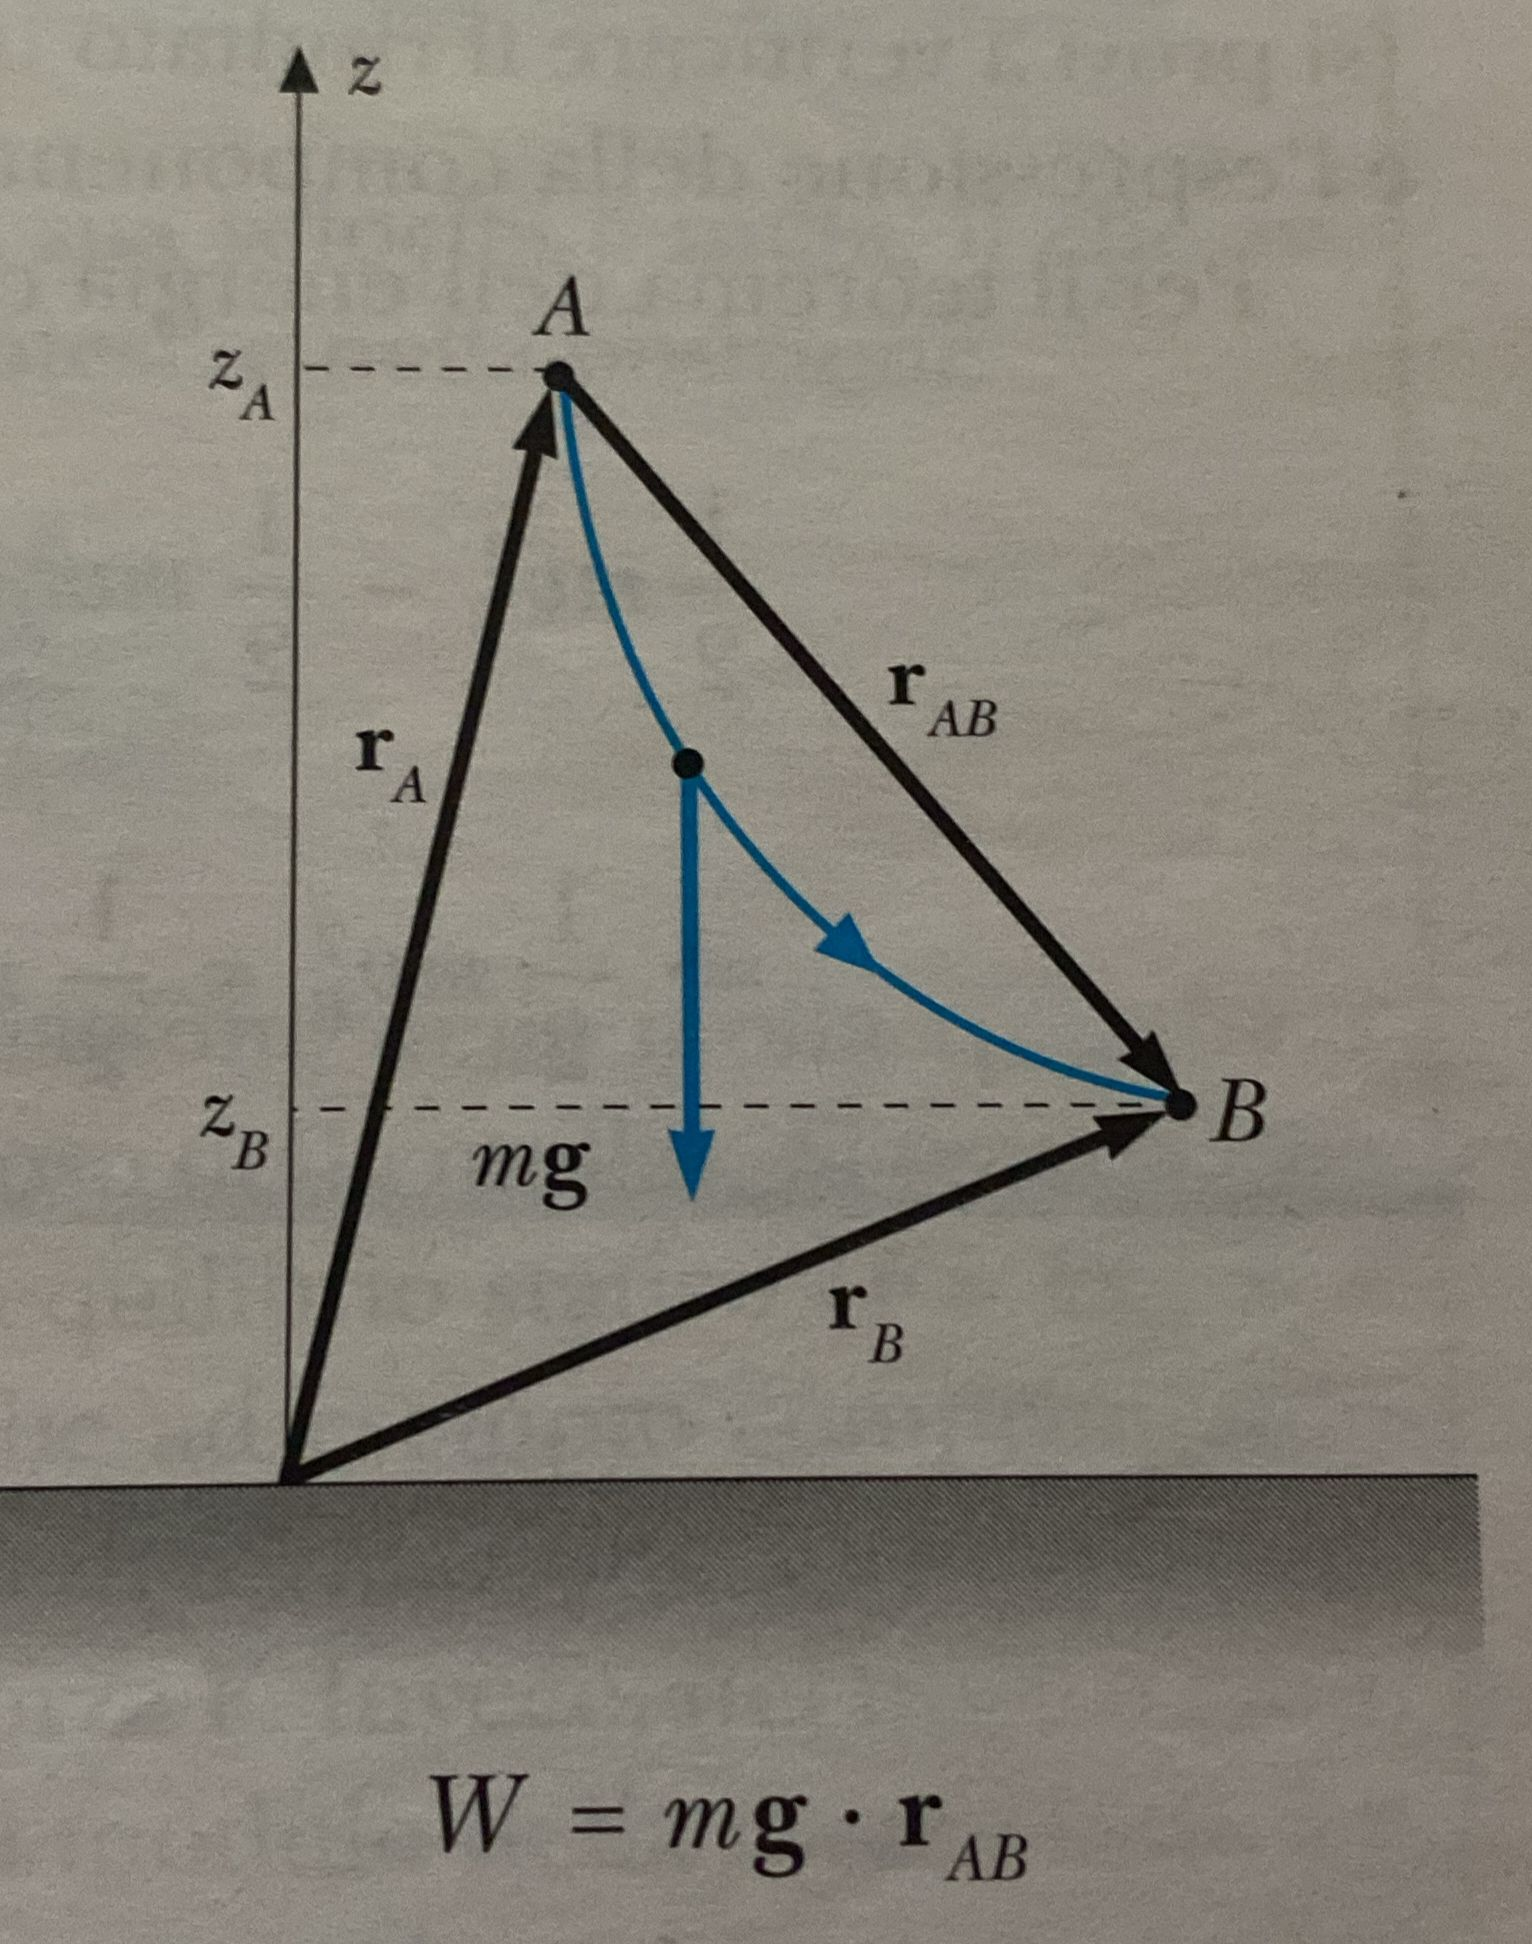
\includegraphics[width=\linewidth]{LavoroForzaPeso.jpeg}}
\end{minipage}%
\hfill
\begin{minipage}[t]{0.55\textwidth}
  \raggedright
Se il punto B si trova in una posizione più bassa di A il lavoro della forza peso è positivo. Se il punto B si trova invece in una posizione più alta di A, $W<0$, $E_P$ aumenta: per fare avvenire questo spostamento bisogna che il punto abbia una sufficiente velocità iniziale così che la diminuzione di energia cinetica eguagli il lavoro oppure bisogna applicare al punto un'altra forza il cui lavoro motore superi in modulo il lavoro resistente della forza peso.
\end{minipage}
\subsubsection{Lavoro di una forza costante}
La trattazione fatta per la forza peso si estende a qualsiasi altra forza costante.
\begin{equation}
    W=-(Fz_B-Fz_A)=-\Delta E_p
\end{equation}
\subsection{Lavoro di una forza elastica}
Il lavoro della forza elastica $\vec{F}=-kx\vec{u}_x$, per uno spostamento lungo l'asse x vale:
\begin{equation}
    W=\int_A^B -kx\vec{u}_x \cdot dx\vec{u_x}=-k \int_A^Bxdx= \frac{1}{2}kx_A^2-\frac{1}{2}kx_B^2=-\Delta E_p
\end{equation}
dove $E_p=\frac{1}{2}kx^2$, funzione solo della posizione, è detta \textbf{energia potenziale elastica}. \textbf{Il lavoro è espresso come l'opposto della variazione dell'energia potenziale tra la posizione finale e iniziale}. Se la coordinata iniziale è maggiore di quella finale, cioè se il punto si muove verso il centro della forza, il lavoro compiuto dalla forza elastica è positivo, $E_p$ diminuisce (spostamento naturale). Nel caso contrario di allontanamento dal centro $W<0$, $E_p$ aumenta: per eseguire tale spostamento il punto deve possedere une velocità iniziale oppure si deve applicare una forza opportuna.
\subsection{Lavoro di una forza di attrito radente}
La forza di attrito radente è data da: ricordando che il vettore $u_v$ è parallelo e concorde allo spostamento ds, il lavoro corrispondente si scrive:
\begin{equation}
    W=\int_A^B\vec{F}_{ad} \cdot ds = \int_A^B -\mu_dN\vec{u}_v \cdot ds=-\mu_dN\int_A^Bds
\end{equation}
dove l'integrale scalare $\int_A^Bds$ è la lunghezza del percorso da A a B, misurata lungo la traiettoria effettiva del punto materiale. Pertanto a parità dei fattori $\mu_d$ e N, abbiamo un lavoro diverso a seconda della forma della traiettoria:\\\\
Il lavoro della forza di attrito radente dipende dal percorso e non è esprimibile come differenza dei valori di una funzione delle coordinate nei punti A e B. \textbf{Il lavoro della forza di attrito radente è sempre negativo} cioè è lavoro resistente.
\subsection{Forze Conservative. Energia Potenziale}
I tre esempi di calcolo di lavoro presentano una differenza sostanziale: nei primi due (forza peso e forza elastica) il lavoro viene a dipendere solo dalle coordinate delle posizioni A e B e non dal particolare percorso che congiunge A e B, nel terzo (forza di attrito) invece il lavoro dipende dalla traiettoria. Le forze del primo tipo, quelle per cui il lavoro non dipende dal percorso, si chiamano \textbf{forze conservative}. Per il calcolo del lavoro possiamo utilizzare qualsiasi percorso che colleghi A e B:
\begin{equation}
    \int_A^B (\vec{F} \cdot d\vec{s})_I=\int_A^B(\vec{F} \cdot d\vec{s})_{II}= \int_A^B \vec{F} \cdot d\vec{s}
\end{equation}
Il lavoro lungo il percorso I coincide con quello lungo il percorso II, o lungo qualsiasi altro e per eseguire il calcolo pratico possiamo così scegliere il percorso analiticamente più comodo. Di conseguenza se si inverte il senso di percorrenza cioè si va da B a A, cambia solo il segno del lavoro. Per un percorso chiuso ABA lungo la traiettoria I e la traiettoria -II si ha che il lavoro è uguale a 0. Di conseguenza \textbf{lungo un qualsiasi percorso chiuso il lavoro è nullo}:
\begin{equation}
    \oint\vec{F}\cdot d\vec{s} = 0
\end{equation}
Questa proprietà si può assumere come definizione di forza conservativa. La funzione delle coordinate di cui abbiamo parlato finora si chiama, come detto, \textbf{energia potenziale} e per tutte le forze conservative vale la reazione:
\begin{equation}
    W=E_{p,A}-E_{p, B}= -\Delta E_p
\end{equation}
Riassumendo:
\begin{itemize}
    \item Per tutte le forze conservative il lavoro si esprime sempre come l'opposto della variazione dell'energia potenziale relativa alla specifica forza
    \item Non esiste una formula generale dell'energia potenziale, ma l'espressione esplicita dell'energia potenziale dipende dalla particolare forza conservativa cui essa si riferisce
    \item Nei due casi che abbiamo discusso si è ottenuto, rispettivamente per la forza peso e per la forza elastica
    \begin{equation}
        E_{p,peso}=mgz \ , \ E_{p,el}=\frac{1}{2}kx^2
    \end{equation}
\end{itemize}
Quando durante il moto l'energia potenziale diminuisce ($\Delta E_p<0$), il lavoro compiuto dalla forza è positivo e può essere utilizzato. Se invece l'energia potenziale aumenta ($\Delta E_p>0$) il lavoro è negativo e ciò in pratica vuol dire che bisogna fornire lavoro dall'esterno per fare avvenire quel determinato processo. \textbf{Da una forza conservativa non si può ricavare lavoro se il percorso è chiuso ovvero, come si dice, se il processo è ciclico}. Le forze per le quali non vale la proprietà di invarianza rispetto al percorso si dicono \textbf{non conservative}, e per esse non si può introdurre l'energia potenziale. Il lavoro di una forza non conservativa si calcola con la 6.1.1 ed è sempre uguale, come per qualsiasi forza, alla variazione di energia cinetica. Una classe particolare di forze non conservative sono le forze di attrito, dette anche \textbf{forze dissipative}.
\subsection{Conservazione dell'energia meccanica}
\begin{equation}
    E_{k,A}+E_{p,A}=E_{k,B}+E_{p,B}
\end{equation}
La somma dell'energia cinetica e dell'energia potenziale di un punto materiale che si muove sotto l'azione di forze conservative resta costante durante il moto, ossia si conserva. Tale somma si chiama \textbf{energia meccanica} per cui l'equazione sopra esprime il \textbf{principio di conservazione dell'energia meccanica}:\\
In presenza di forze conservative l'energia meccanica di un punto materiale si conserva
\begin{equation}
    E_m=E_k+E_p=costante
\end{equation}
Il lavoro ottenuto a spese della diminuzione di energia potenziale causa un aumento dell'energia cinetica e viceversa dato che la somma delle energie è costante. Durante il moto avviene una trasformazione da una forma di energia all'altra, per tramite di lavoro compiuto e assorbito, ma il contenuto energetico totale, dato dall'energia meccanica non cambia.
\begin{equation}
    W_{nc}=(E_{k,B}+E_{p,B})-(E_{k,A}+E_{p,A})=E_{m,B}-E_{m,A}
\end{equation}
\textbf{In presenza di forze non conservative l'energia meccanica non resta costante e la sua variazione è eguale al lavoro delle forze non conservative.} Generalmente quindi l'energia meccanica non si conserva ma diminuisce a causa di effetti dissipativi come l'attrito.
\subsection{Momento angolare. Momento della forza}
Si definisce come \textbf{momento angolare} il momento del vettore quantità moto
\begin{equation}
    \vec{L}= \vec{r} \times \vec{p} = \vec{r} \times m\vec{v}
\end{equation}
ed è l'equivalente rotazionale della quantità di moto. Se un oggetto ruota intorno a un punto, ha momento angolare rispetto a quel punto. Indica quanto e in che modo l’oggetto sta ruotando. Più il corpo è massiccio, veloce o lontano dal centro di rotazione, maggiore è il suo momento angolare.
Il \textbf{momento della forza} è definito come:
\begin{equation}
    \vec{M} = \vec{r} \times \vec{F}
\end{equation}
\subsubsection{Teorema del momento angolare}
\begin{equation}
    \frac{d\vec{L}}{dt}=\vec{M}
\end{equation}
Questa relazione rappresenta \textbf{il teorema del momento angolare} per un punto materiale:\\\\
La derivata temporale del momento angolare è eguale al momento della forza se entrambi i momenti sono riferiti allo stesso polo fisso in un sistema di riferimento inerziale.\\\\
\textbf{Il momento angolare di un punto materiale rimane costante nel tempo, si conserva, se il momento delle forze è nullo.}\\
\textbf{Teorema del momento dell'impulso:}
\begin{equation}
    \int_0^t \vec{M}dt = \int_0^t (\vec{r} \times \vec{F})dt = \vec{r} \times \int_0^t \vec{F} dt = \vec{r} \times \vec{J} = \Delta \vec{L}
\end{equation}
La variazione di momento angolare è eguale al momento dell'impulso applicato al punto.
\begin{equation}
    W=\int_A^B F_T ds = \int_{\theta_A}^{\theta_B} rF_T d\theta=\int_{\theta_A}^{\theta_B} M d\theta
\end{equation}
\subsection{Alcune osservazioni sulla dinamica del punto}
La \textbf{legge fondamentale} da utilizzare per lo studio del moto di un punto materiale è $\vec{F}=m\vec{a}=m \frac{d\vec{v}}{dt}$. A tal fine si devono identificare le forze che effettivamente agiscono sul punto, non dimenticando reazioni vincolari, tensioni di fili o eventuali attriti. Si deve inoltre valutare lungo quali direzioni può essere più conveniente scomporre le forze, facendo particolare attenzione a non commettere errori di segno proiettando. In generale velocità e accelerazione non sono parallele e il moto avviene nella direzione e verso della velocità, non dell'accelerazione e quindi della forza. Conseguenza diretta della seconda legge di Newton è che il \textbf{lavoro della forza agente è eguale alla variazione dell'energia cinetica del punto su cui agisce la forza}. Il significato dell'\textbf{energia}, sia cinetica che potenziale, è \textbf{la capacità di un sistema di scambiare lavoro} ovvero essa va intesa come \textbf{serbatoio di lavoro}. Il fatto che un punto materiale possieda una certa energia potenziale o cinetica implica che con opportuni processi si può ricavare lavoro, parzialmente o integralmente a seconda che ci siano o non ci siano attriti. Un'applicazione molto comune del \textbf{principio di conservazione dell'energia meccanica} sfrutta il legame tra l'energia cinetica funzione della velocità e l'energia potenziale , funzione delle coordinate, per esprimere la velocità in funzione della posizione. Questa via normalmente è da preferire nei problemi in cui non è richiesta la dipendenza dal tempo. Se invece è richiesta esplicitamente la legge oraria conviene applicare la legge di Newton.
\section{Moti Relativi}
\subsection{Sistemi di riferimento, velocità e accelerazione relative}
Sperimentalmente è provato con estrema accuratezza che le leggi fisiche non dipendono dalla scelta del sistema di riferimento. Non esiste pertanto un punto privilegiato dello spazio e nemmeno un'orientazione privilegiata: lo spazio appare omogeneo e isotropo. La situazione si presenta diversa quando un fenomeno viene osservato da due sistemi di riferimento in moto l'uno rispetto all'altro. Non sussiste invarianza delle leggi fisiche rispetto a due sistemi di riferimento in moto qualsiasi l'uno rispetto all'altro.
\subsubsection{Teorema delle velocità relative }
\begin{figure}[H]
    \centering
    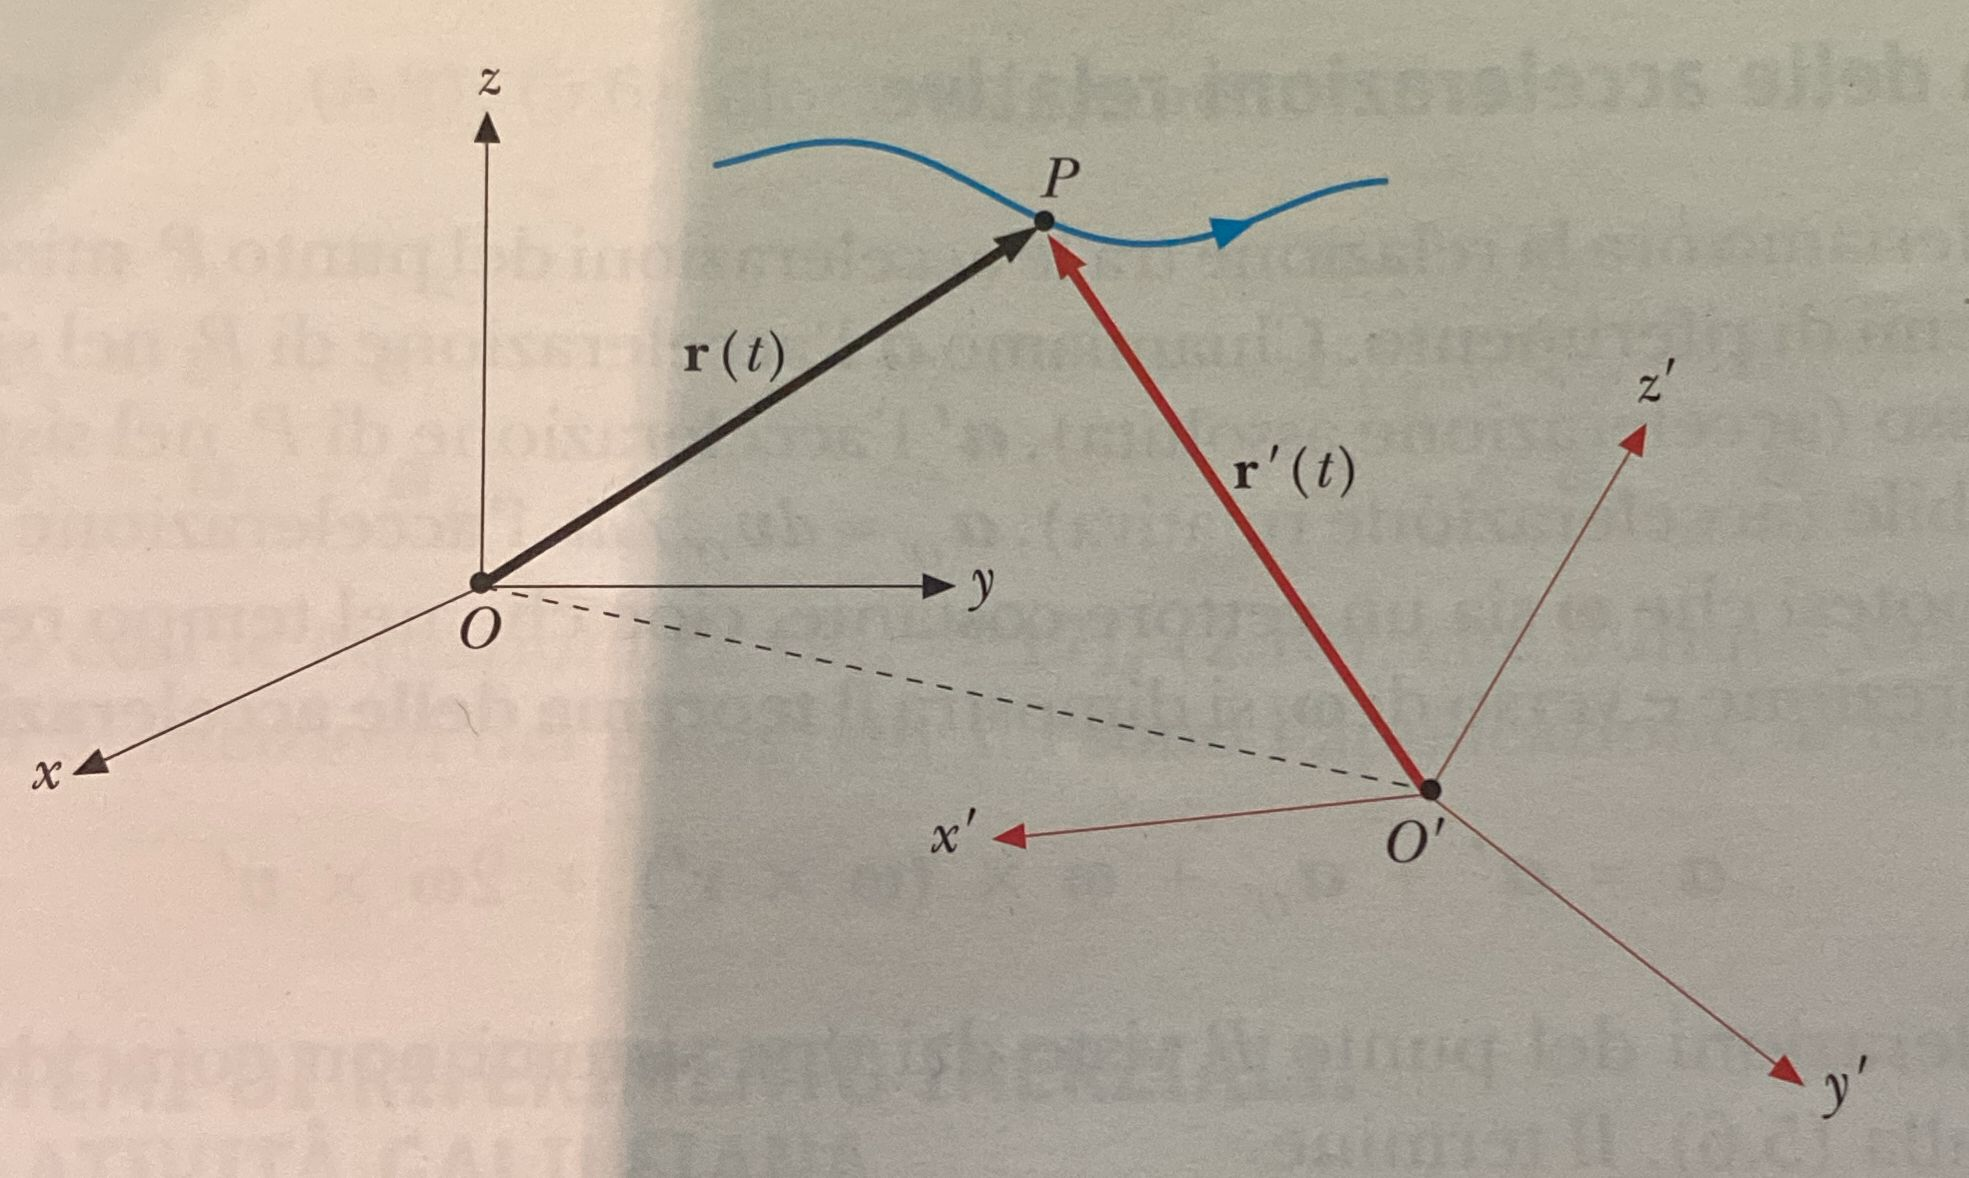
\includegraphics[width=0.5\linewidth]{MotiRelativi.jpeg}
    \caption{Sistema di riferimento fisso (nero) e in moto (rosso)}
    \label{fig:enter-label}
\end{figure}
Viene rappresentato un punto P lungo una generica traiettoria. Il suo moto viene osservato da una terna cartesiana con centro in O che, per convenzione, chiamiamo \textbf{sistema di riferimento fisso} e da una terna cartesiana con centro O' che, sempre per convenzione, chiamiamo \textbf{sistema di riferimento mobile.} L'origine del sistema mobile ha una velocita $v_0$, rispetto al sistema fisso; inoltre l'insieme dei tre assi mobili, che è assimilabile ad un corpo indeformabile, in generale ruota con velocità angolare \textbf{$\omega$}. Vogliamo trovare le relazioni che esistono tra la posizione, la velocità e l'accelerazione del punto P, misurate da un'osservatore solidale con il sistema fisso e con il sistema mobile. La relazione tra le posizioni del punto P, misurate rispetto ai due sistemi di riferimento, è la seguente:
\begin{equation}
    \vec{r}=\vec{OO} + \vec{r'}
\end{equation}
Detta v la velocità di P rispetto al sistema fisso e v' la velocità di P rispetto al sistema mobile, si dimostra il seguente \textbf{teorema delle velocità relative}:
\begin{equation}
    \vec{v}=\vec{v'}+\vec{v_{O'}}+ \vec{\omega} \times \vec{r'}
\end{equation}
Le velocità del punto P viste dai due sistemi in moto relativo sono diverse, però sono correlate grazie alla formula soprascritta. Il termine correttivo, chiamato \textbf{velocità di trascinamento}, è:
\begin{equation}
    \vec{v_t}=\vec{v}-\vec{v'}=\vec{v_{O'}} + \vec{\omega} \times \vec{r'}
    \end{equation}
    Ci sono poi due casi particolari importanti:
    \begin{itemize}
        \item Il sistema mobile non ruota rispetto a quello fisso ($\omega$=0); si parla di \textbf{moto relativo traslatorio} tra i due sistemi, ovvero di \textbf{moto di trascinamento traslatorio}:
        \begin{equation}
            \vec{v}=\vec{v'}+\vec{v_{O'}} \ \ , \  \ \vec{v_t}=v_{O'}
        \end{equation}
        \item Il sistema mobile non si sposta rispetto a quello fisso ($v_0$=0), ma ruota:
        \begin{equation}
            \vec{v}=\vec{v'} + \vec{\omega} \times \vec{r'} \ \ , \ \ \vec{v_t}=\vec{\omega} \times \vec{r'}
        \end{equation}
        si parla di \textbf{moto relativo rotatorio} tra i due sistemi, ovvero di \textbf{moto di trascinamento rotatorio.}
    \end{itemize}
\subsubsection{Teorema delle accelerazioni relative}
\begin{equation}
    \vec{a}=\vec{a}' + \vec{a_{O'}} + \vec{\omega} \times (\vec{\omega} \times \vec{r}') + 2\vec{\omega} \times \vec{v}'
\end{equation}
Le accelerazioni del punto P viste dai due sistemi non coincidono ma sono correlate. Introduciamo l'\textbf{accelerazione di trascinamento} e dipende, come $v_t$, dai parametri del moto relativo tra i due sistemi e dalla posizione di P nel sistema mobile.
\begin{equation}
    \vec{a_t}=\vec{a_{O'}}+\vec{\omega} \times (\vec{\omega} \times \vec{r}')
\end{equation}
Introduciamo poi l'\textbf{accelerazione complementare} o di \textbf{Coriolis} e dipende dal moto di P rispetto al sistema mobile ($\vec{v}'$). Quindi:
\begin{equation}
    \vec{a}=\vec{a}'+\vec{a_t}+\vec{a_c}
\end{equation}
In corrispondenza ai due casi particolari già evidenziati per la velocità abbiamo:
\begin{align}
    & \vec{a}=\vec{a}'+\vec{a_{O'}} \\
    & \vec{a} = \vec{a}' + \vec{\omega} \times (\vec{\omega} \times \vec{r}') + 2\vec{\omega} \times \vec{v}'
\end{align}
\subsubsection{Velocità e accelerazione di un punto rispetto ad un altro}
Oltre al moto di un punto visto da due sistemi di riferimento, è necessario talvolta considerare il moto di un punto $P_2$ rispetto ad un altro punto $P_1$. \\
\begin{minipage}[t]{0.4\textwidth}
  \raisebox{-\height}{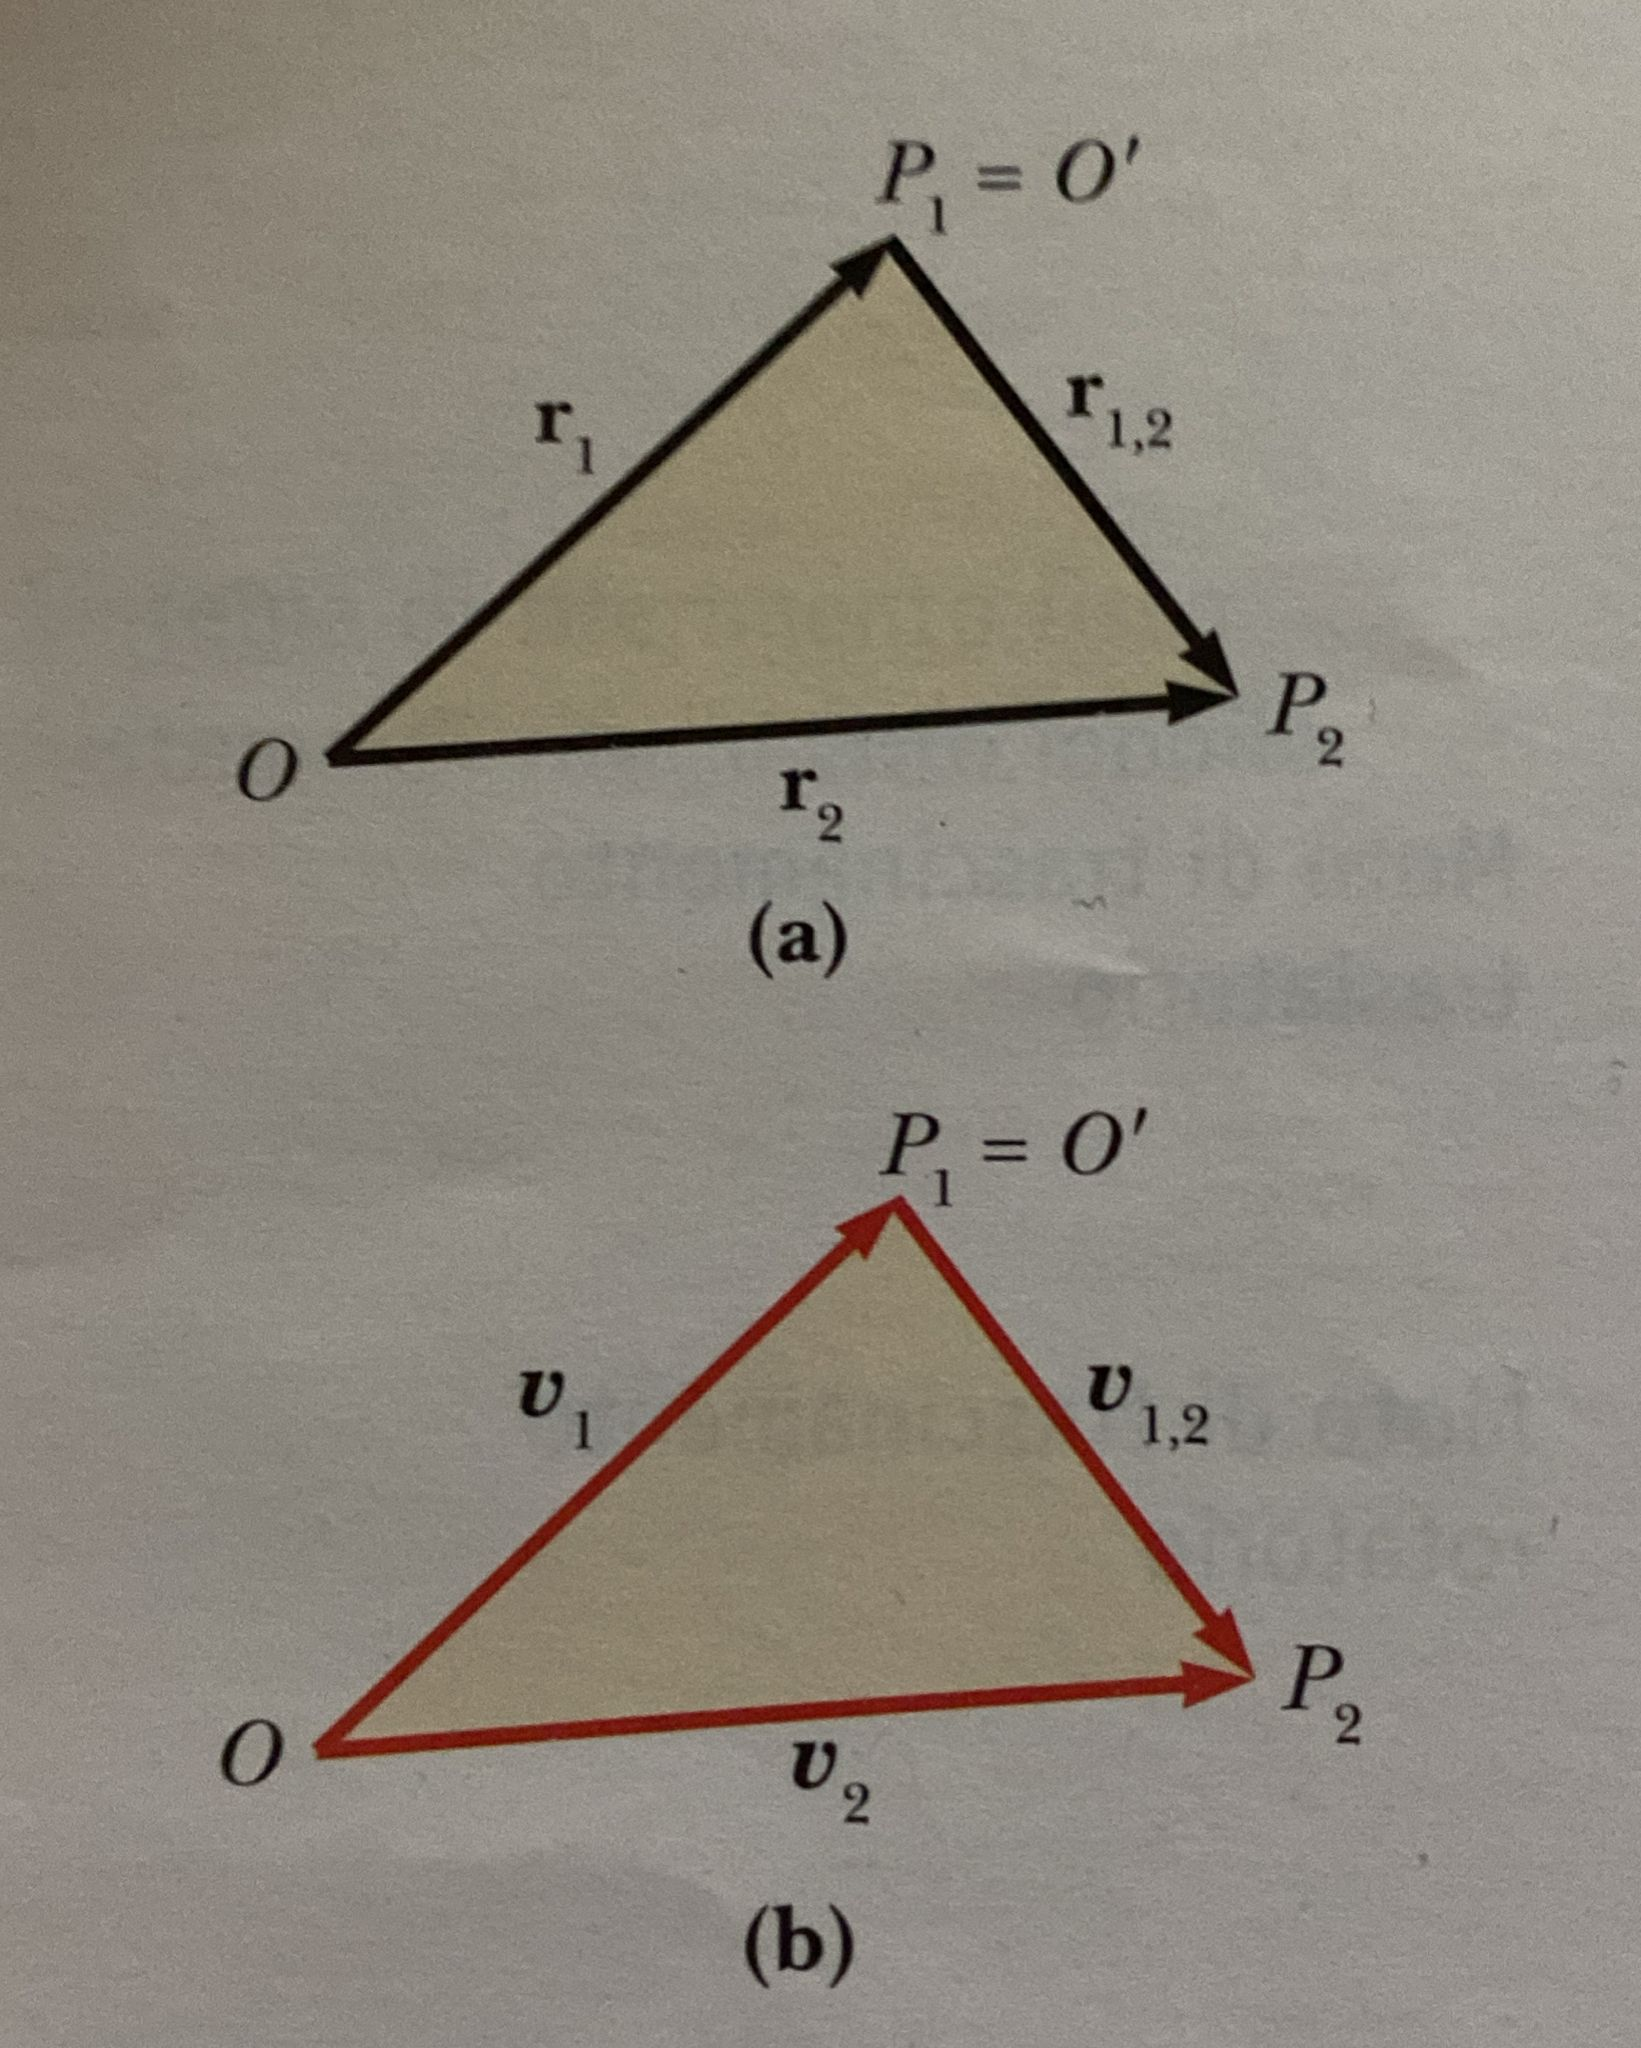
\includegraphics[width=\linewidth]{SpostamentiRelativi.jpeg}}
\end{minipage}%
\hfill
\begin{minipage}[t]{0.55\textwidth}
  \raggedright
\begin{align*}
    &  \ \ punto \ \ P_2 \ \ rispetto \ \ ad \ \ O \ \ \ \ \ \ \vec{r}=\vec{r_2} \ \ , \ \ \vec{v}=\vec{v_2} \ \ , \ \ \vec{a}=\vec{a_2} \\
    & \ \ punto \ \ P_2 \ \ rispetto \ \ ad \ \ O' \ \ \ \ \ \ \vec{r}'=\vec{r_{1,2}} \ \ , \ \ \vec{v}'=\vec{v_{1,2}} \ \ , \ \ \vec{a}'=\vec{a_{1,2}} \\
    & \ \ punto \ \ P_1 \ \ rispetto \ \ ad \ \ O \ \ \ \ \ \ \vec{r}=\vec{r_2} \ \ , \ \ \vec{v}=\vec{v_2} \ \ , \ \ \vec{a}=\vec{a_2} \\
    & \ \ \vec{r_2}=\vec{r_1}+ \vec{r_{1,2}} \ \ -> \ \ \vec{r_{1,2}}=\vec{r_2}-\vec{r_1} \\
    & \ \ \vec{v_2}=\vec{v_1}+ \vec{v_{1,2}} \ \ -> \ \ \vec{v_{1,2}}=\vec{v_2}-\vec{v_1} \\
    & \ \ \vec{a_2}=\vec{a_1}+ \vec{a_{1,2}} \ \ -> \ \ \vec{a_{1,2}}=\vec{a_2}-\vec{a_1} \\
    \end{align*}
\end{minipage}
\subsection{Sistemi di riferimento inerziali. Relatività Galileiana}
Definiamo come \textbf{sistema di riferimento inerziale} un sistema in cui valga rigorosamente la legge di inerzia, in cui cioè un punto non soggetto a forze lanciato con velocità arbitraria in qualunque direzione si muova con moto rettilineo uniforme o, se è in quiete, resti in quiete. È ragionevole supporre che questa situazione si verifichi sia quando il punto è sufficientemente lontano da ogni altro corpo in modo da poter trascurare ogni interazione, sia quando è possibile bilanciare le forze agenti in modo che la risultante sia nulla. Consideriamo ora un altro sistema di riferimento che si muove di moto traslatorio rettilineo uniforme rispetto ad un certo sistema inerziale. Pertanto si ha:
\begin{equation}
    \vec{v_{O'}}=costante \ \ ,\ \ \vec{a_{O'}}=0 \ \ e \ \ \vec{\omega}=0 , \ \ \vec{a}=\vec{a}'
\end{equation}
Le accelerazioni di un punto misurate nei due sistemi di riferimento sono eguali. Se $\vec{a}=0$ anche $\vec{a}'=0$ e quindi pure il secondo sistema è inerziale. Abbiamo così ottenuto questo risultato fondamentale: \textbf{definito un sistema di riferimento inerziale, tutti gli altri sistemi in moto rettilineo uniforme rispetto a questo sono anch'essi inerziali}. Per tali sistemi la legge di Newton si scrive allo stesso modo. Conseguenza importante è che, essendo la dinamica la stessa, non è possibile stabilire, tramite misure effettuate in questi diversi sistemi di riferimento, se uno di essi è in quiete o in moto. Non ha senso cioè il concetto di moto assoluto. Tale situazione fisica viene descritta anche con il termine di \textbf{relatività galileiana}. Se il moto del secondo sistema è accelerato rispetto al sistema inerziale, sia perchè $\vec{a_{O'}}\neq0$ oppure $\vec{\omega}=0$ o per entrambe le ragioni, si osserva che la legge di Newton non è più valida, la \textbf{forza vera} che agisce sul punto considerato non è proporzionale all'accelerazione del punto, misurata nel sistema accelerato. Se $\vec{F}=m\vec{a}$ nel sistema inerziale, nel sistema mobile in moto accelerato non può sussistere la relazione $\vec{F}=m\vec{a}'$ poichè $\vec{a}'\neq \vec{a}$.
\begin{equation}
    \vec{F}-m\vec{a_t}-m\vec{a_c}=m\vec{a}'
\end{equation}
Questa equazione rappresenta una forma modificata dalla legge di Newton: in un sistema non inerziale il prodotto della massa del punto materiale per l'accelerazione misurata in quel sistema è eguale alla \textbf{forza vera} agente sul punto più le \textbf{forze apparenti}. Queste ultime forze, che sono sempre proporzionali alla massa del punto vengono chiamate \textbf{forze di inerzia}, appaiono agenti solo nel sistema non inerziale, dove costituiscono il termine correttivo che permette di ritornare ad una espressione $\vec{F}'=m\vec{a}'$. È chiaro che \textbf{le forze apparenti non derivano dalle interazioni fondamentali e non esistono in un sistema di riferimento inerziale.} In un sistema accelerato vediamo che $\vec{F}=0$ non comporta $\vec{a}'=0$ e quindi l'osservazione di un moto rettilineo uniforme. Questo risultato giustifica il nome di sistema non inerziale per un sistema accelerato. Analogamente, una traiettoria curva non presuppone necessariamente l'azione di una forza (vera), ma può essere un effetto apparente, conseguenza del moto accelerato del sistema in cui si trova l'osservatore, e così via. Nei prossimi paragrafi presenteremo vari esempi di moti osservati da due sistemi di riferimento diversi, di cui almeno uno inerziale. Assumeremo come inerziale il sistema con origine O, mentre l'altro avrà origine in O' e metteremo in evidenza cosa misurano due osservatori, detti per brevità O e O', solidali con i due sistemi.
\subsection{Moto di trascinamento traslatorio rettilineo}
\begin{minipage}[t]{0.4\textwidth}
  \raisebox{-\height}{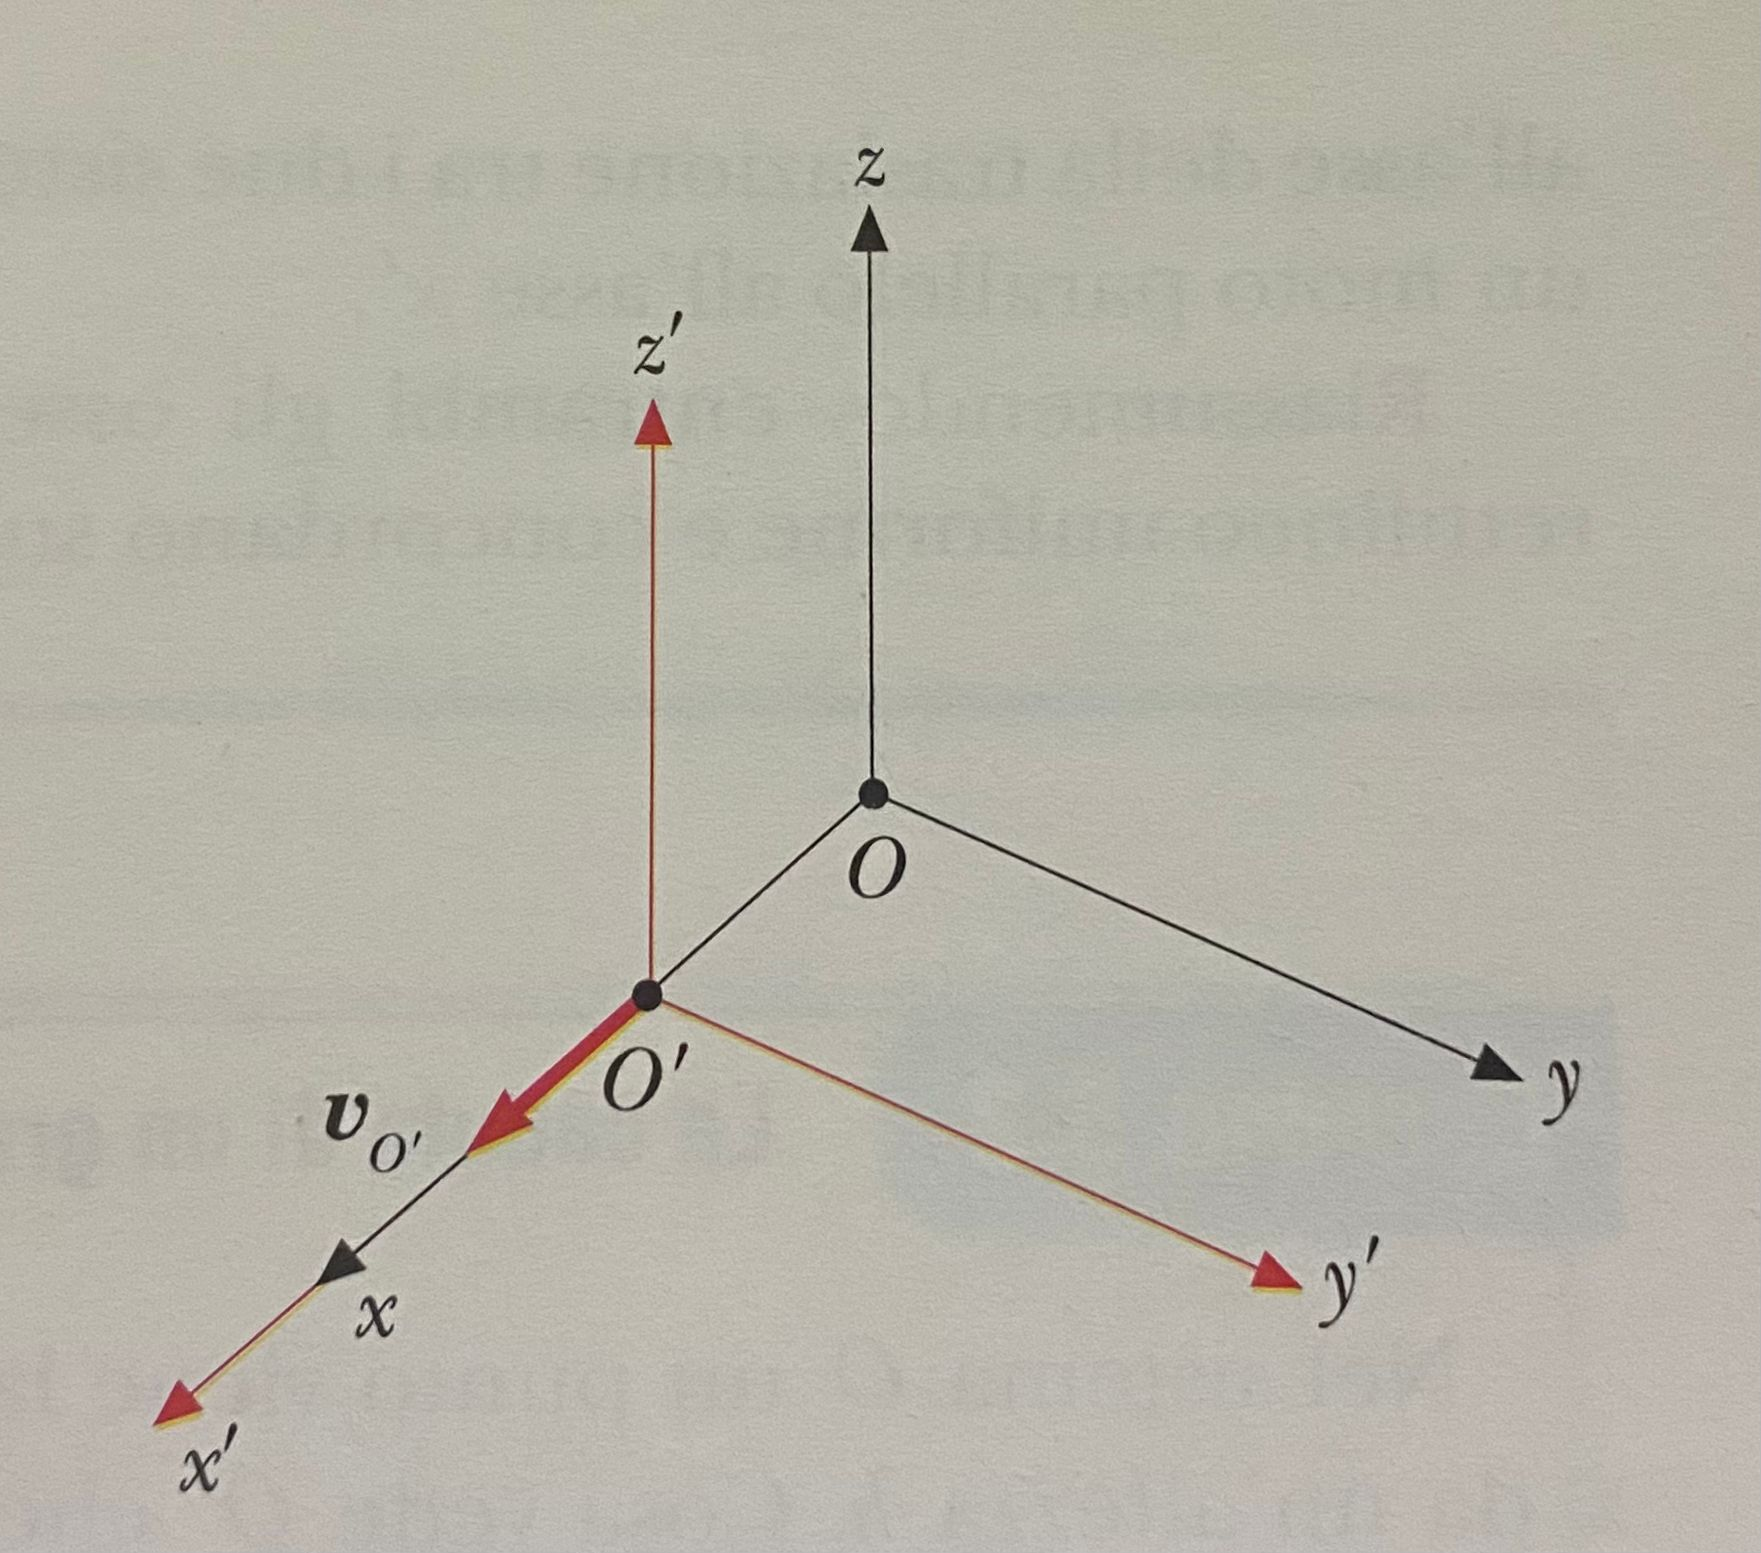
\includegraphics[width=\linewidth]{MotoDiTrascinamentoTraslatorioRettilineo.jpeg}}
\end{minipage}%
\hfill
\begin{minipage}[t]{0.55\textwidth}
  \raggedright
Consideriamo il moto di trascinamento traslatorio più semplice, che è quello rettilineo (O' si muove rispetto a O lungo una traiettoria rettilinea) e ci mettiamo nella situazione della figura. Si presentano due possibilità: il moto di O' è uniforme ($\vec{a_0}=0$) e quindi anche O' è un sistema inerziale, il moto di O' è vario ($\vec{a}_0\neq0$) ovvero O' è un sistema non inerziale. 
\end{minipage}
Nel primo caso (O e O' entrambi sistemi di riferimento inerziali), le relazioni per velocità e accelerazione sono:
\begin{equation}
    \vec{v}=\vec{v}'+\vec{v_0} \ \ , \ \ \vec{a}=\vec{a}'
\end{equation}
mentre il legame tra i raggi vettori è:
\begin{equation}
    \vec{r}=\vec{v_0}t + \vec{r}'
\end{equation}
infatti $\vec{OO'}=\vec{v_0}t$. Le relazioni vettoriali possono essere proiettate sugli assi cartesiani fornendo le relazioni tra le componenti dei vettori:
\begin{align*}
    & x'=x-v_0t \ \ \ \ y'=y \ \ \ \ z'=z \\
    & v_x'=v_x-v_0 \ \ \ \ v_y'=v_y \ \ \ \ v_z'=v_z \\
    & a_x'=a_x \ \ \ \ a_y'=a_y \ \ \ \ a_z'=a_z \\
\end{align*}
Queste trasformazioni di grandezze tra due sistemi entrambi inerziali si chiamano \textbf{trasformazioni galileiane}. Passiamo adesso al caso in cui O sia un sistema di riferimento inerziale e O' un sistema di riferimento non inerziale. Assumiamo la stessa configurazione geometrica e supponiamo per semplicità che O' abbia un'accelerazione costante $\vec{a_O}=\vec{a_t}$ e una velocità iniziale $\vec{v}_{in}$, ambedue parallele e concordi all'asse $x\equiv x'$. La posizione e la velocità di O' sono quindi espresse da:
\begin{equation}
    x_{O'}=v_{in}t + \frac{1}{2}a_tt^2 \ \ \ ,\  \ \ v_{O'}=v_{in}+a_tt
\end{equation}
Le formule di trasformazione diventano:
\begin{align*}
    & \vec{r'}=\vec{r}-\vec{OO'} \ \ \ \ x'=x-v_{in}t-\frac{1}{2}a_tt^2 \ \ \ \ y'=y \ \ \ \ z'=z \\
    & \vec{v'}=\vec{v}-\vec{v_0} \ \ \ \ v_x'=v_x-v_{in}-a_tt \ \ \ \ v_y'=v_y \ \ \ \ v_z'=v_z \\
    & \vec{a'}=\vec{a}-\vec{a_0} \ \ \ \ a_x'=a_x-a_t \ \ \ \ a_y'=a_y \ \ \ \ a_z'=a_z \\
\end{align*}
Caratteristica distintiva è la diversità delle accelerazioni nei due sistemi, O inerziale e O' non inerziale, e quindi la diversità delle forze agenti, con conseguente comparsa delle forze d'inerzia.
\subsection{Moto di trascinamento rotatorio uniforme}
Supponiamo ora che il moto di trascinamento sia soltanto rotatorio uniforme e per comodità prendiamo coincidenti le origini dei due sistemi ($\vec{r}=\vec{r'}$). Abbiamo $\vec{v}_0=0,\vec{a_0}=0, \omega=costante$, e le relazioni diventano:
\begin{equation}
    \vec{v}=\vec{v'}+ \vec{\omega} \times \vec{r}
\end{equation}
\begin{equation}
    \vec{a}=\vec{a'}+ \vec{\omega} \times (\vec{\omega} \times \vec{r}) + 2 \vec{\omega} \times \vec{v}'
\end{equation}
Abbiamo quindi:
\begin{equation}
    \vec{F}+\vec{F}_{centr} + \vec{F}_{Cor}= m\vec{a}'
\end{equation}
la \textbf{forza centrifuga}, $\vec{F}_{centr}=-m\vec{\omega} \times (\vec{\omega} \times \vec{r})$, e la \textbf{forza di Coriolis}, $\vec{F}_{Cor}=-2m\vec{\omega} \times \vec{v}'$, hanno lo stesso ruolo della forza $-m\vec{a}_t$, vista nel paragrafo precedente.
\begin{figure}[H]
    \centering
    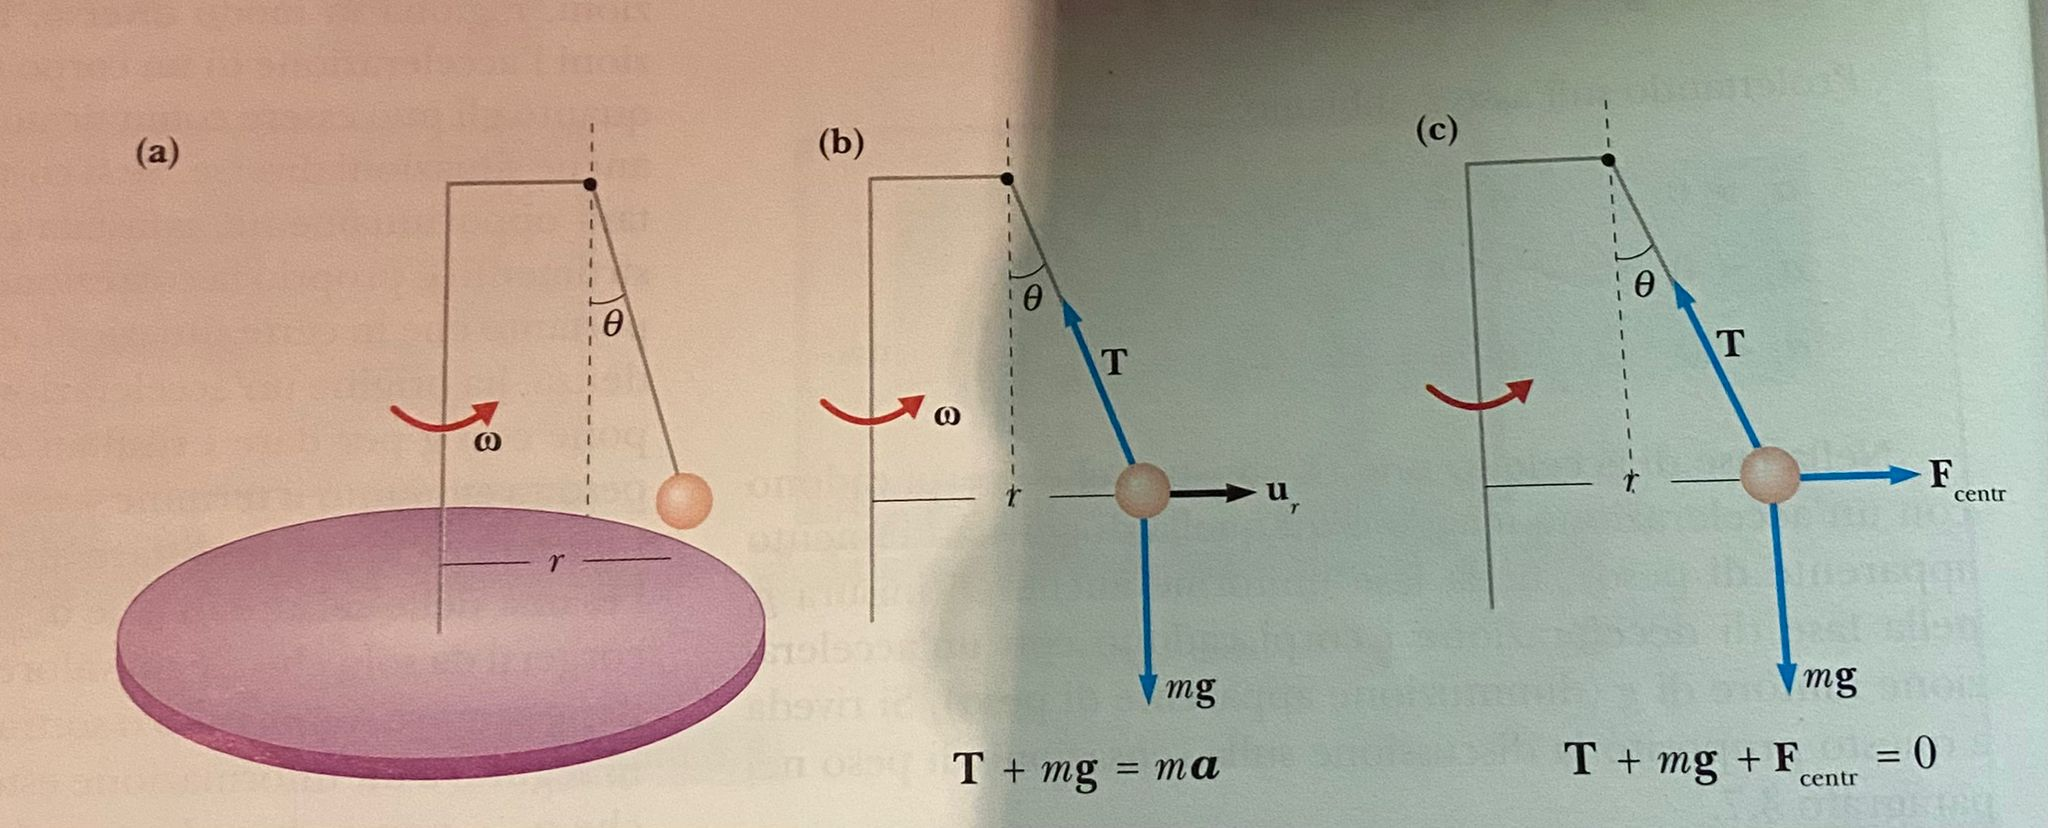
\includegraphics[width=0.5\linewidth]{MotoDiTrascinamentoRotativoUniforme.jpeg}
    \caption{Filo a piombo fissato su una piattaforma rotante (a); analisi delle forze sul filo a piombo per un osservatore inerziale (b) e per un osservatore sulla piattaforma (c)}
    \label{fig:enter-label}
\end{figure}
\noindent
Il filo a piombo si dispone secondo una direzione inclinata di un angolo $\theta$ rispetto alla verticale, crescente con la velocità angolare e con la distanza r dall'asse di rotazione. Il punto materiale non si muove rispetto alla piattaforma, dunque $v'=0$ e $\vec{F}_{Cor}=0$. Per un osservatore inerziale, il moto di rotazione del punto materiale è determinato dalle forze vere ovvero dalla forza peso mg e dalla tensione del filo:
\begin{equation}
    \vec{T}+m\vec{g}=m\vec{a}=-m\omega^2r\vec{u}_r
\end{equation}
Dalla b:
\begin{equation}
    Tsen\theta=m\omega^2r \ \ , \ \ Tcos\theta=mg \ \ , \  \ tg\theta=\frac{a}{g}=\frac{\omega^2r}{g}
\end{equation}
La \textbf{forza centripeta} richiesta per mantenere in rotazione il punto materiale su una circonferenza di raggio r è fornita dalla componente orizzontale della tensione T del filo. Per un'osservatore O' sulla piattaforma, figura c, il punto materiale è fermo, per cui:
\begin{equation}
    \vec{T}+m\vec{g}+\vec{F}_{centr}=O \ \ \ -> \ \ \ F_{centr}=-m\vec{a}=m\omega^2r\vec{u}_r
    \end{equation}
Le forze vere sono equilibrate dalla forza centrifuga $F_{centr}=m\omega^2r\vec{u}_r$ apparente. Va ripetuto che le forze d'inerzia, non hanno esistenza reale in quanto non derivano dalle interazioni fondamentali e non compaiono nella descrizione del moto effettuata in un sistema di riferimento inerziale.
\subsection{Alcuni commenti}
\subsubsection{Il moto rispetto alla terra}
Nei paragrafi precedenti abbiamo introdotto la nozione di sistema inerziale senza però darne un esempio: lo facciamo adesso, dicendo che un sistema di riferimento con l'origine nel centro di massa del sistema solare e gli assi diretti verso determinate \textbf{stelle fisse} è con ottima approssimazione un sistema inerziale, come lo sono tutti gli altri sistemi in moto rettilineo uniforme rispetto ad esso. Qualsiasi calcolo accurato di traiettorie, effettuato in un sistema terrestre, deve tener conto degli effetti delle forze d'inerzia.
\subsubsection{Relatività galileiana}
Proprietà fondamentali dei sistemi di riferimento inerziali:
\begin{itemize}
    \item La dinamica di un fenomeno viene spiegata utilizzando soltanto le forze vere, che derivano dalle interazioni fondamentali
    \item Quando un fenomeno viene osservato da due sistemi inerziali l'interpretazione dinamica è la stessa
\end{itemize}
In particolare non si può decidere quale dei due sistemi sia in moto e quale sia fermo, non ha significato il concetto di moto assoluto. Questo risultato, che prende il nome di \textbf{relatività galileiana}, trova una espressione analitica nelle formule di trasformazione, che mettono in relazione le misure di posizione, velocità e accelerazione eseguite in due sistemi inerziali.
\section{Dinamica dei sistemi di punti materiali}
\subsection{Sistemi di punti. Forze interne e Forze esterne}
Consideriamo un sistema di n punti materiali, con n maggiore di 1, interagenti tra di loro e con il resto dell'universo. La forza $\vec{F}_i$ agente sull'i-esimo punto si può pensare come risultante delle \textbf{forze esterne} agenti sul punto, $\vec{F}_i^{(E)}$, e delle forze esercitate dagli altri n-1 punti, \textbf{forze interne} al sistema, $\vec{F}_i^{(I)}$:
\begin{equation}
    \vec{F}_i=F_i^{(E)} + F_i^{(I)}
\end{equation}
\begin{minipage}[t]{0.4\textwidth}
  \raisebox{-\height}{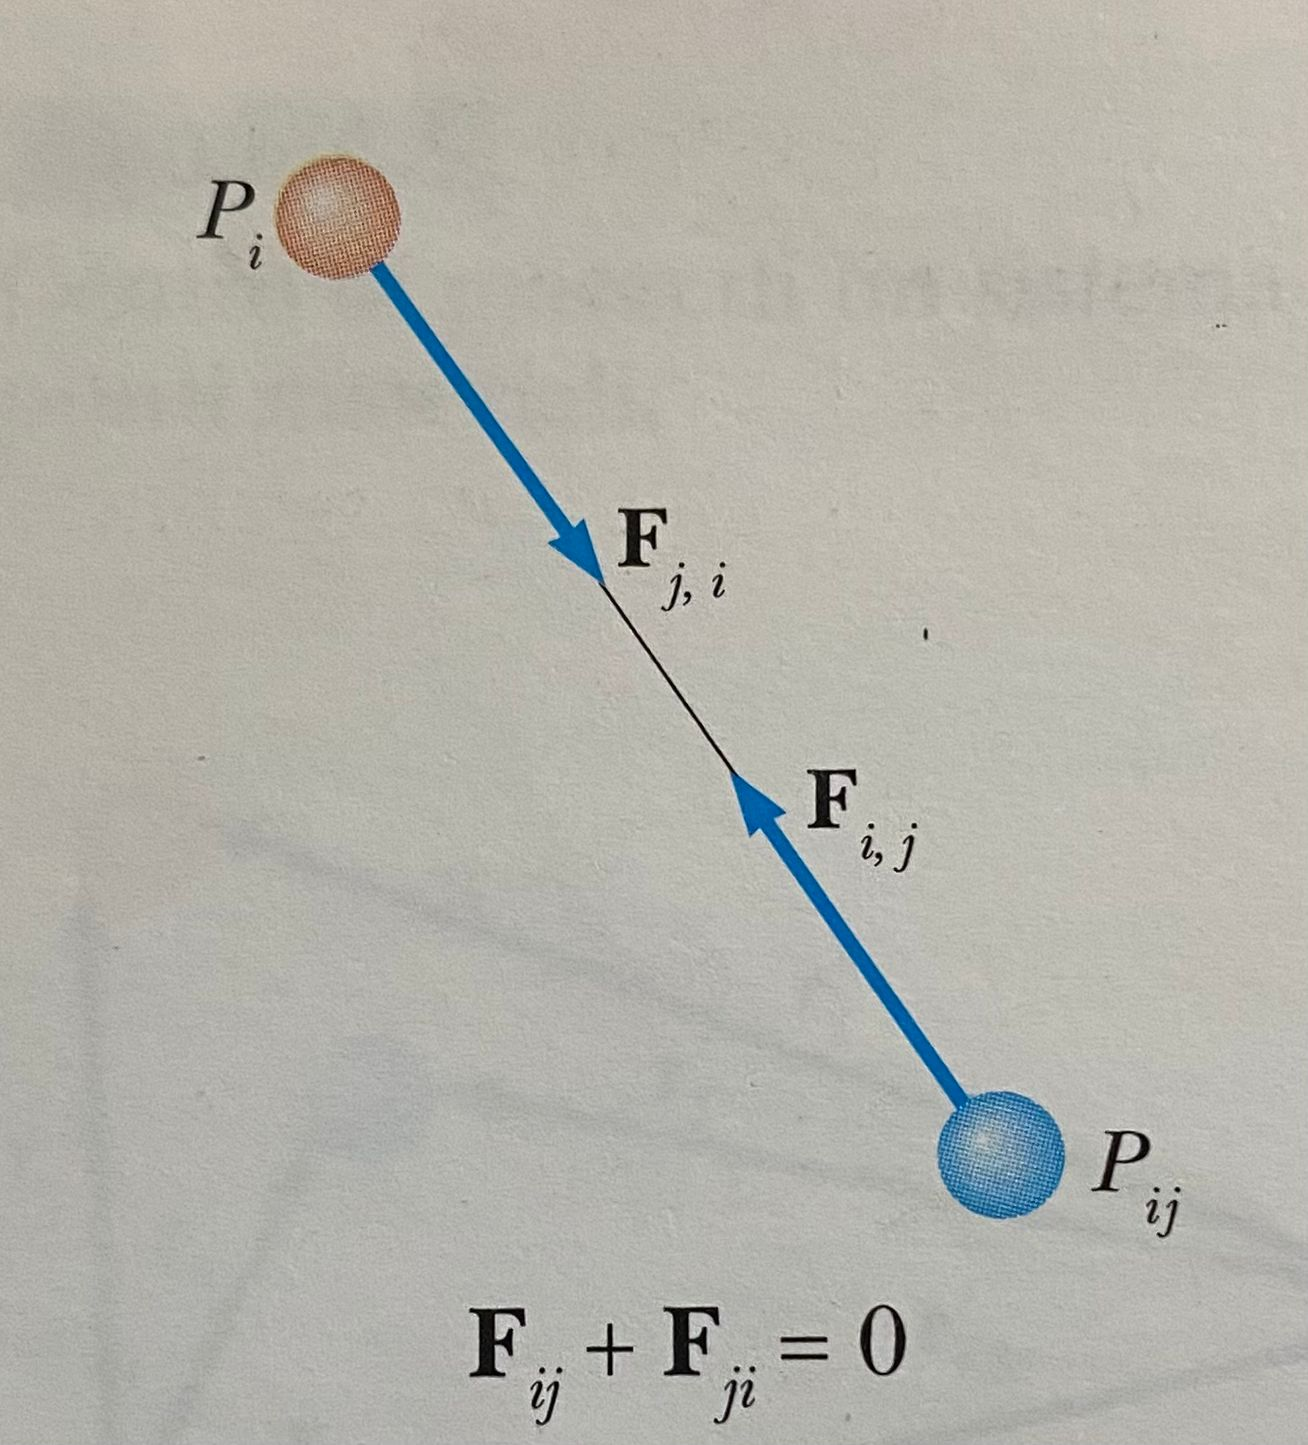
\includegraphics[width=0.7\linewidth]{ForzeAttrattive.jpeg}}
  \raisebox{-\height}{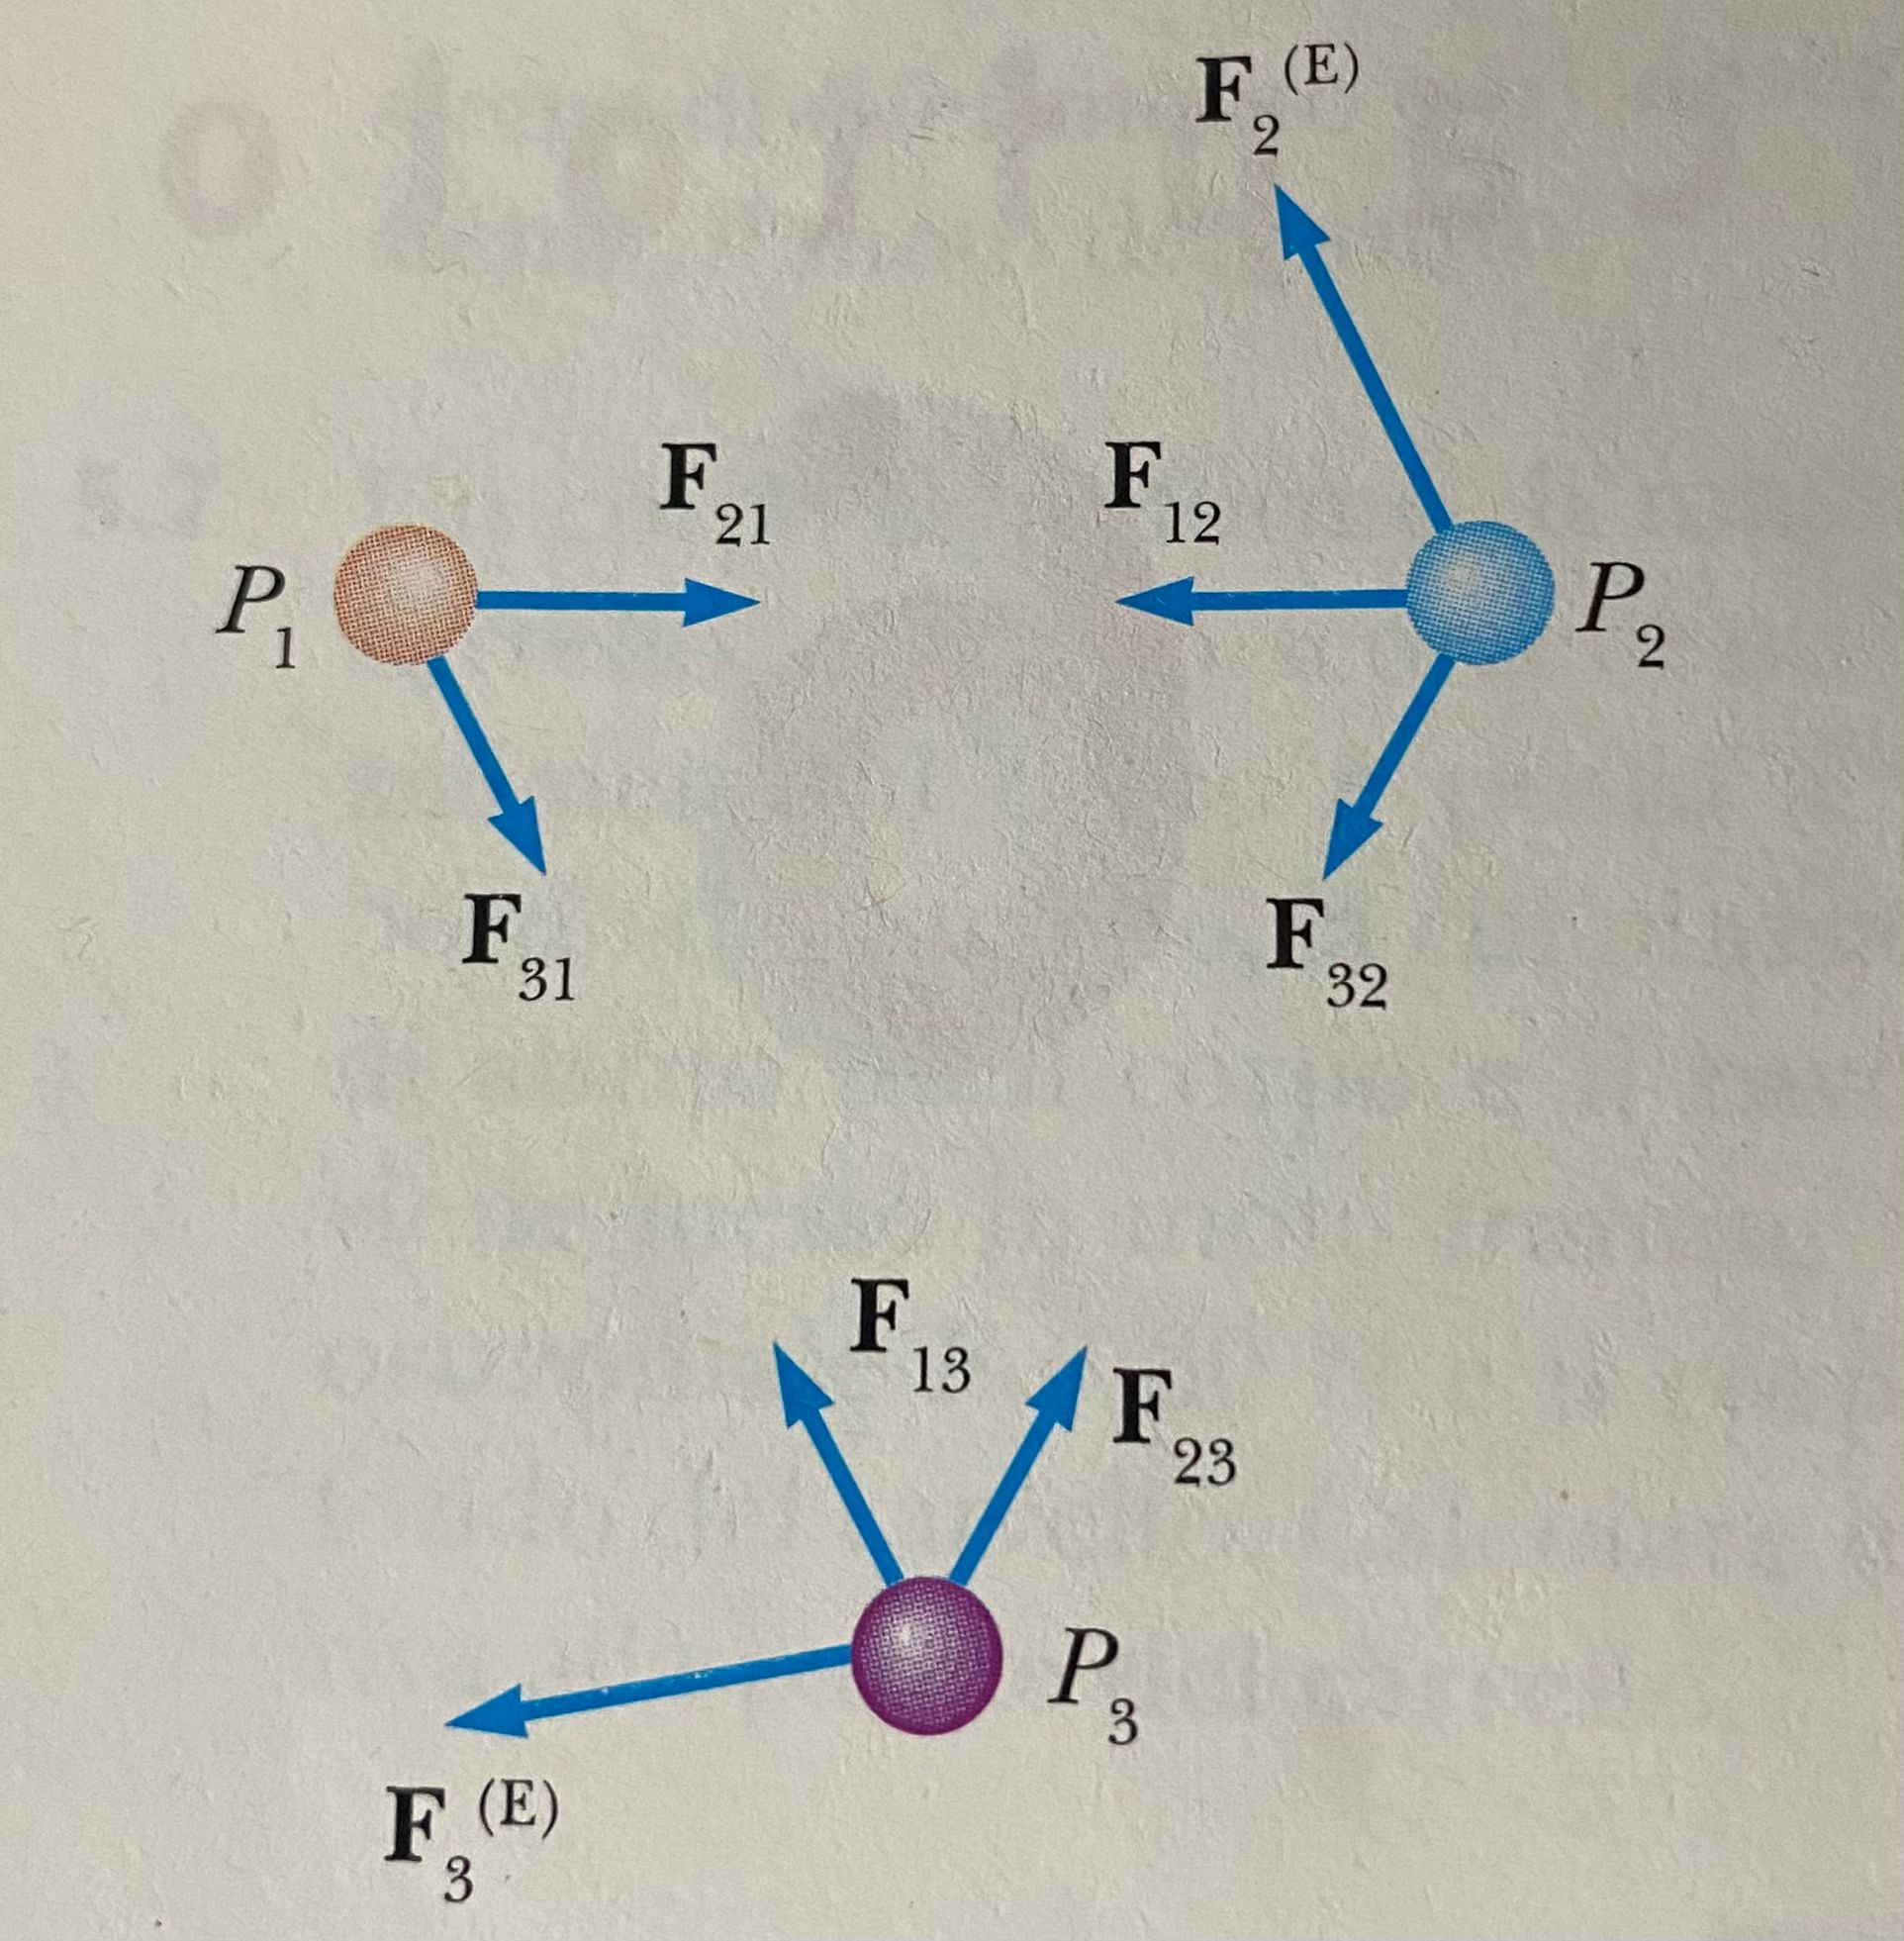
\includegraphics[width=0.7\linewidth]{SistemaDiTrePunti.jpeg}}
\end{minipage}%
\hfill
\begin{minipage}[t]{0.55\textwidth}
  \raggedright
La distinzione tra forze interne ed esterne dipende da come viene definito il sistema di punti. Alle \textbf{forze interne si applica la terza legge di Newton, o principio di azione e reazione} 
che richiamiamo: se il punto i-esimo esercita una forza sul punto j-esimo la forza $\vec{F}_{i,j}$, il punto j-esimo reagisce esercitando sul punto i-esimo la forza $\vec{F}_{j,i}$ e tali forze hanno la stessa retta di azione, stesso modulo e verso opposto; esse possono essere attrattive o repulsive, in figura un esempio di attrattive. La seconda figura riporta una possibile configurazione si forze interne ed esterne per un generico sistema di tre punti. In generale, la risultante $\vec{F}_i^{(I)}$ delle forze interne agenti sull'i-esimo punto è diversa da zero, però \textbf{la risultante di tutte le forze interne del sistema è nulla} perchè, in base al principio di azione e reazione, esse sono a due a due eguali ed opposte. 

\end{minipage}
\newpage
Per ciascun punto $P_i$ di massa $m_i$ sottoposto alla forza $\vec{F_i}$ consideriamo le grendezze misurate in un sistema di riferimento inerziale:
\begin{align}
    & posizione \ \ \ \ \vec{r}_i \ \ \ \ \ \ \text{velocità} \ \ \ \ \vec{v_i} \\
    & accelerazione \ \ \ \ \vec{a}_i= \vec{F}_i/m_i \ \ \ \ \ \ \text{quantità} \  di \  moto \ \ \ \ \vec{P_i}=m_i\vec{v}_i \\
    & momento \ angolare \ \ \ \ \vec{L}_i=\vec{r}_i \times m_i\vec{v_i} \ \ \ \ \ \ energia \ cinetica \ \ \ \ \vec{E}_{k,i}=\frac{1}{2}m_i\vec{v}_i^2  \\
\end{align}
Per il sistema complessivo di punti possiamo inoltre definire le grandezze:
\begin{align}
    & \text{quantità} \ \ di \ moto \ totale \ \ \ \ \vec{P}=\sum_iP_i=\sum_i m_i\vec{v}_i \\
    & momento \ angolare \ totale \ \ \ \ \vec{L}= \sum_i \vec{L}_i= \sum_i \vec{r}_i \times m_i \vec{v}_i  \\
    & energia \ cinetica \ totale \ \ \ \ \vec{E}_k= \sum_iE_{k,i}=\sum_i\frac{1}{2}m_i\vec{v}_i^2  \\
\end{align}
I momenti angolari vanno riferiti a un polo, che nelle formule è stato preso coincidente con l'origine, ma che può essere un qualsiasi altro punto, fermo o in movimento, nel sistema di riferimento inerziale.
\newpage
\subsection{Centro di massa di un sistema di punti. Teorema del moto del centro di massa.}
\begin{figure}[H]
    \centering
    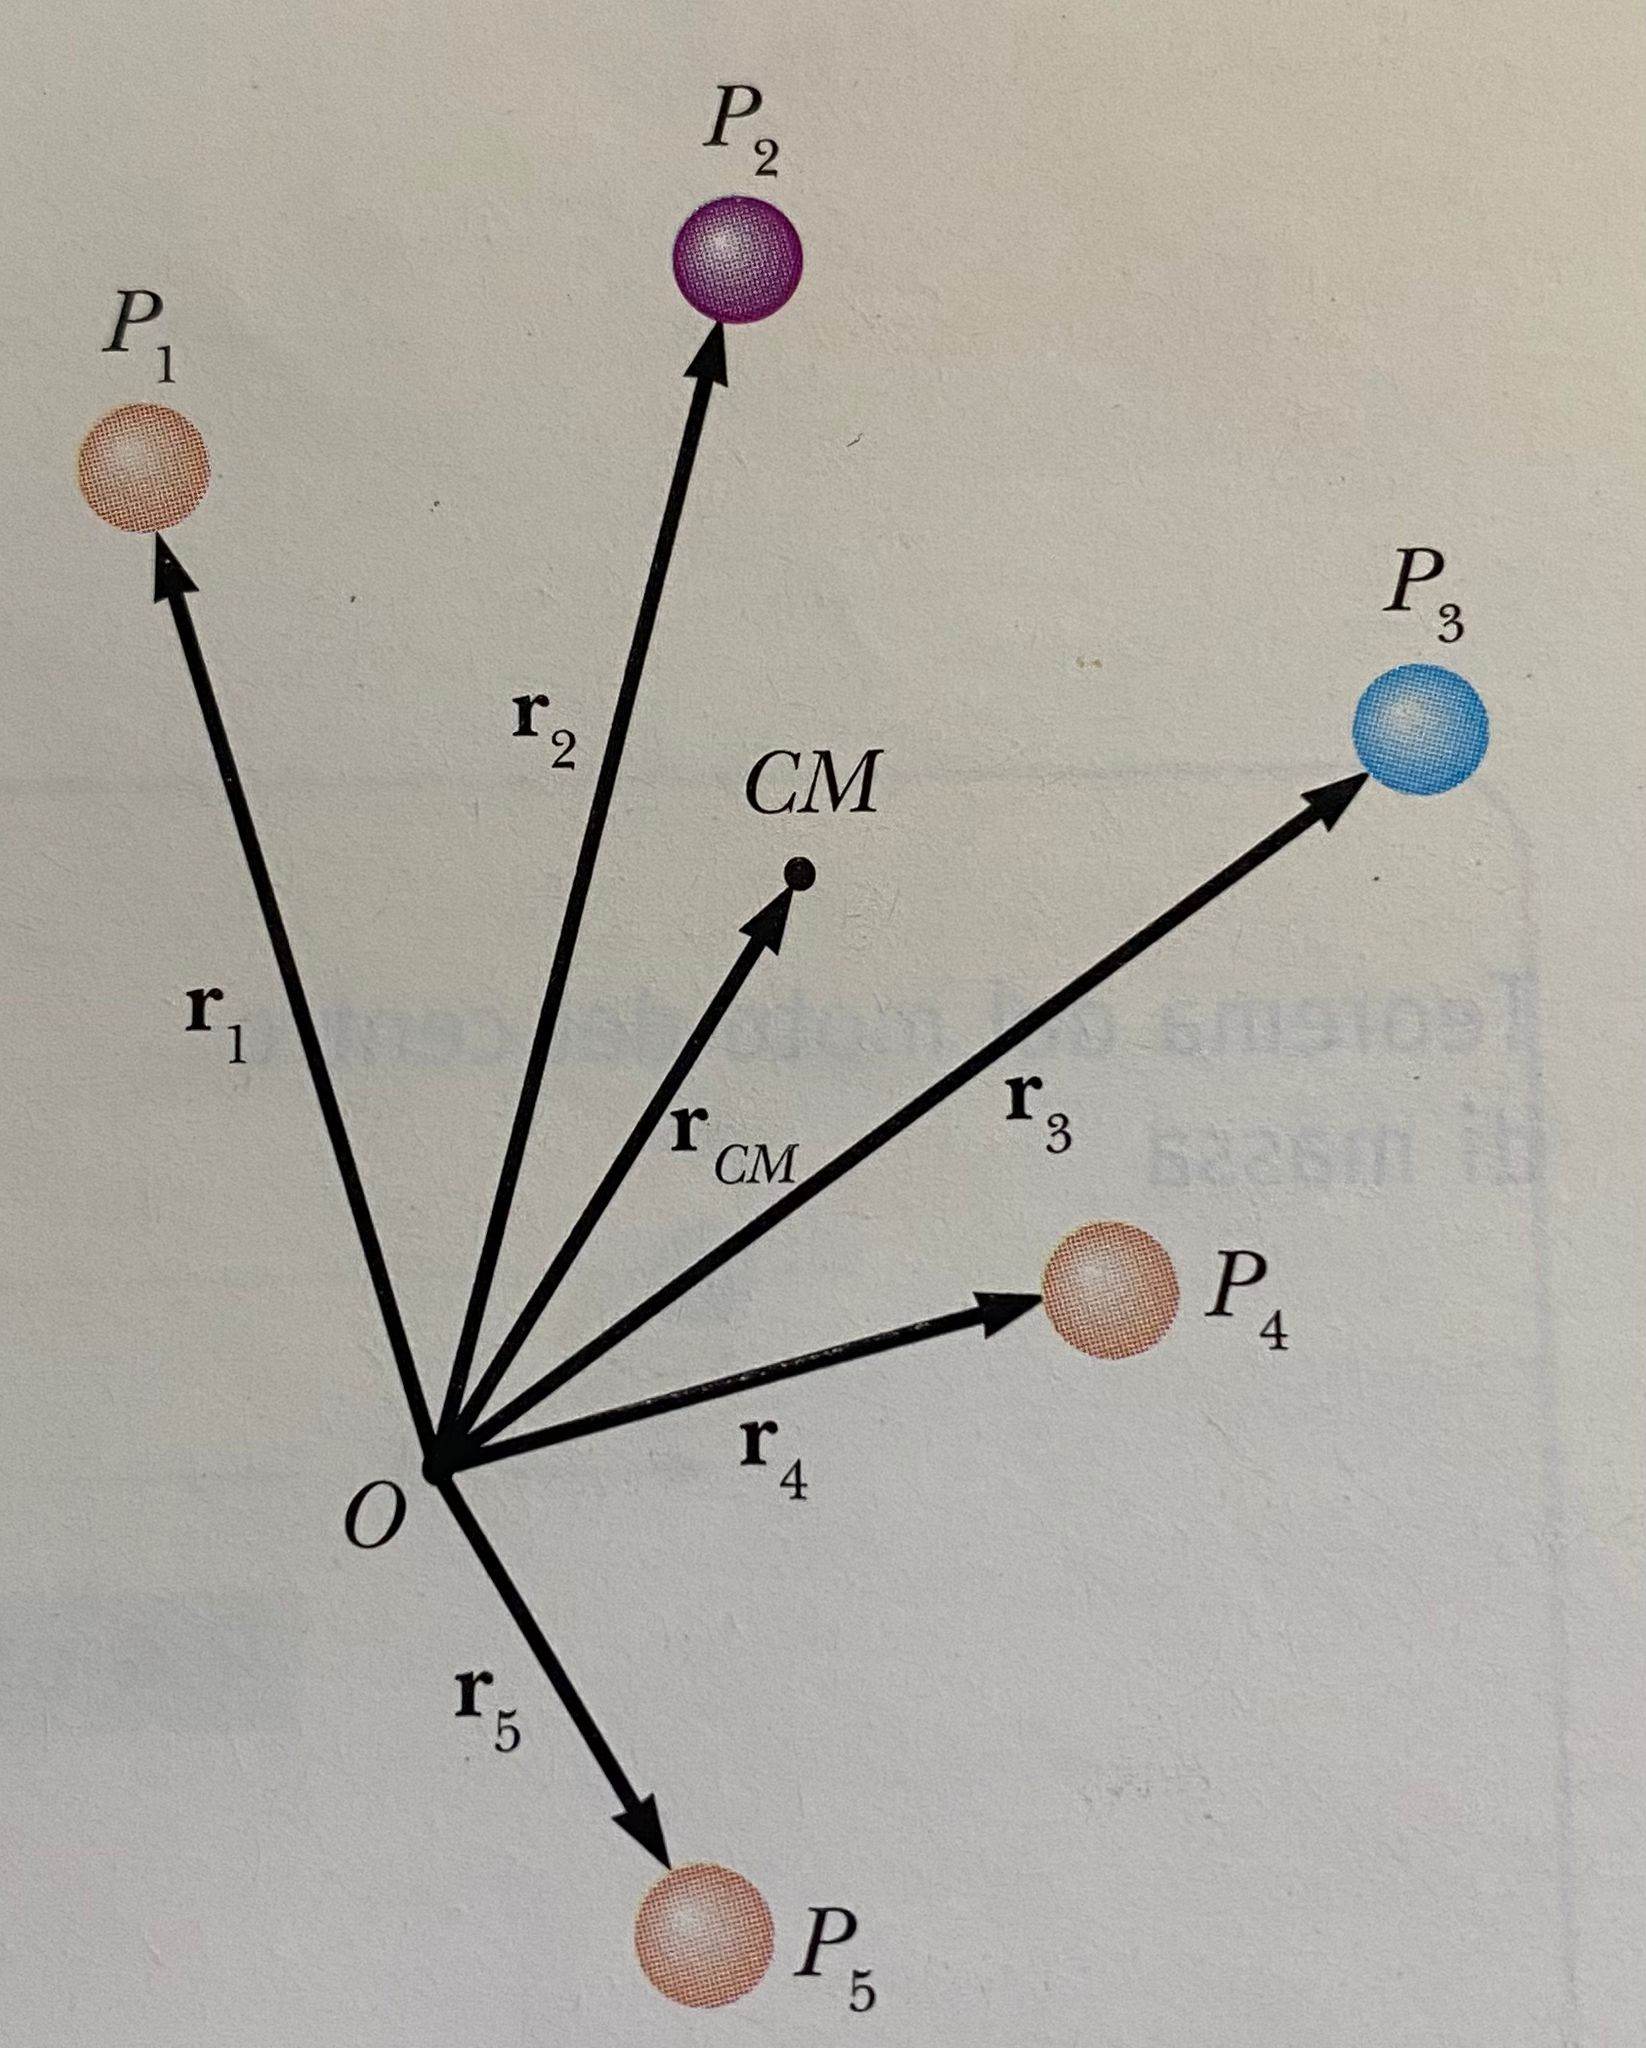
\includegraphics[width=0.25\linewidth]{CentroDiMassa.jpeg}
    \caption{Centro di massa di un sistema di punti materiali}
    \label{fig:enter-label}
\end{figure}
\noindent
Si definisce \textbf{centro di massa di un sistema di punti materiali}, il punto geometrico la cui posizione è individuata, nel sistema di riferimento considerato, dal raggio vettore:
\begin{equation}
    \vec{r}_{CM}= \frac{\sum_im_i\vec{r}_i}{\sum_im_i}
\end{equation}
Le componenti di $\vec{r}_{CM}$, ovvero le coordinate del centro di massa in un sistema di coordinate cartesiane con l'origine O, sono:
\begin{equation}
    x_{CM}=\frac{\sum_im_ix_i}{\sum_im_i}  \ \ , \ \ y_{CM}=\frac{\sum_im_iy_i}{\sum_im_i} \ \ , \ \ z_{CM}=\frac{\sum_im_iz_i}{\sum_im_i}
\end{equation}
Si noti che la posizione del centro di massa rispetto agli n punti materiali non dipende dal sistema di riferimento, mentre le sue coordinate invece variano a seconda del sistema prescelto. Introduciamo poi la \textbf{velocità del centro di massa:}
\begin{equation}
    \vec{v}_{CM}=\frac{d\vec{r}_{CM}}{dt}=\frac{\sum_im_i\frac{dr_i}{dt}}{\sum_im_i}=\frac{\sum_im_i\vec{v}_i}{\sum_im_i}=\frac{\vec{P}}{m}
\end{equation}
Quindi: La quantità di moto di un sistema di punti materiali è eguale alla quantità di moto $m\vec{v}_{CM}$ del centro di massa, considerato come un punto materiale che abbia la posizione $\vec{r}_{CM}$, la velocità $\vec{v}_{CM}$ e massa pari alla massa totale m del sistema. Ricaviamo analogamente l'\textbf{accelerazione del centro di massa:}
\begin{equation}
     \vec{a}_{CM}=\frac{d\vec{v}_{CM}}{dt}=\frac{\sum_im_i\frac{dv_i}{dt}}{\sum_im_i}=\frac{\sum_im_i\vec{a}_i}{\sum_im_i}=\frac{\sum_im_i\vec{a}_i}{m}
\end{equation}
La relazione:
\begin{equation}
    \vec{R}^{(E)}=m\vec{a}_{CM}
\end{equation}
esprime \textbf{il teorema del centro di massa:} Il centro di massa si muove come un punto materiale in cui sia concentrata tutta la massa del sistema e a cui sia applicata la risultante delle forze esterne.
\begin{equation}
    \vec{R}^{(E)}=m\vec{a}_{CM}=m\frac{d\vec{v}_{CM}}{dt}=\frac{d}{dt}(m\vec{v}_{CM})=\frac{d\vec{P}}{dt}
\end{equation}
La risultante delle forze esterne è eguale alla derivata rispetto al tempo della quantità di moto totale del sistema. Il moto del centro di massa è determinato dunque solo dalle forze esterne. L'azione delle forze interne non può modificare lo stato di moto del centro di massa; Invece il moto di ciascun punto dipende dall'azione delle forze esterne ed interne agenti su di esso.
\subsubsection{Osservazioni ed esempi sulle proprietà del centro di massa}
Per ora è stato dimostrato che considerando il centro di massa alla stregua di un punto materiale di massa m, eguale alla massa totale del sistema: \\
\begin{itemize}
    \item La sua velocità è eguale alla quantità di moto totale divisa per la massa totale, ovvero la sua quantità di moto $m\vec{v}_{CM}$ è eguale alla quantità di moto totale $\vec{P}$
    \item La sua accelerazione è determinata dalla risultante delle forze esterne agenti sul sistema. 
    \end{itemize}
In questo senso, facendo riferimento a $\vec{P}$ e $\vec{R}^{(E)}$, possiamo dire che il centro di massa rappresenta il moto globale o di insieme dei punti materiali. Il fatto che ad un certo istante $\vec{v}_{CM}$ abbia un determinato valore significa solamente che il sistema in media si sta spostando in quella data direzione, anche se nessuna delle singole $v_i$ coincide con $\vec{v}_{CM}$. Analogamente, il fatto che $\vec{a}_{CM}$ abbia un certo valore a causa dell'azione di $\vec{R}^{(E)}$ indica che nel suo complesso il sistema sta accelerando in quella data direzione. Il calcolo di $\vec{r}_{CM}$ si può effettuare associando gruppi di punti a piacere, determinando per ciascun gruppo il relativo centro di massa, considerando quest'ultimo come un punto materiale in cui è posta la massa totale del gruppo calcolando infine il centro di massa di tali centri di massa parziali.
\subsection{Conservazione della quantità di moto}
Se il sistema di punti considerato è isolato, cioè non soggetto a forze esterne, oppure l'azione delle forze esterne è tale che la loro risultante $\vec{R}^{(E)}$ sia nulla, abbiamo:
\begin{equation}
    \vec{a}_{CM}=0 \ \ ,\ \ \vec{v}_{CM}=costante \ \ , \ \ \vec{P}=costante
\end{equation}
Tale risultato esprime \textbf{il principio della conservazione della quantità di moto} per un sistema di punti materiali: 
\noindent
\colorlet{shadecolor}{orange!15}
\begin{shaded}
Quando la risultante delle forze esterne è nulla, la quantità di moto totale del sistema rimane costante nel tempo e il centro di massa si muove di moto rettilineo uniforme o resta in quiete
\end{shaded}
Osserviamo inoltre che la conservazione delle quantità di moto può avvenire anche parzialmente, cioè essere riferita a una o due delle componenti. Per esempio se $R_x^{(E)}=0$, allora $P_x=costante$. Notiamo poi che, pur verificandosi $R^{(E)}=0$, le quantità di moto dei vari punti $m_i\vec{v}_i$ in generale variano nel tempo; resta costante solo la loro somma $\sum_im_i\vec{v}_i$. Il principio di conservazione della quantità di moto per un sistema isolato di due punti ha come conseguenza che le forze che si esercitano tra i due punti sono eguali in modulo e di verso opposto. Tale risultato non è completamente equivalente al principio di azione e reazione in quanto $\vec{F}_1=-\vec{F}_2$ non implica che le due forze abbiano la stessa retta di azione. Fatta questa precisazione, potremmo dire che c'è equivalenza tra conservazione della quantità di moto e principio di azione e reazione, generalizzabile a sistemi più complessi. È possibile misurare il valore di una qualsiasi massa, rispetto ad una massa campione, attraverso misure di velocità.
\subsection{Teorema del momento angolare}
Prima di spiegare il teorema, faccio un piccolo recap del momento angolare e degli argomenti a lui collegati.
\subsubsection{Cos'è il momento angolare?}
Il \textbf{momento angolare} è una grandezza fisica che descrive la \textbf{quantità di moto rotazionale} di un oggetto che ruota intorno a un punto o a un asse. Rappresenta l'\textbf{equivalente rotazionale della quantità di moto}. Immagina una pattinatrice sul ghiaccio che ruota su sé stessa con le braccia aperte. Se poi chiude le braccia, ruota più velocemente. Perché? Perché sta conservando il momento angolare!
Anche se cambia la velocità, la quantità totale di "rotazione" rimane costante. Nel caso di un punto materiale corrisponde a:
\begin{equation}
    \vec{L}= m \vec{v} \times \vec{r}
\end{equation}
\subsubsection{Teorema del momento angolare per un punto materiale}
Il \textbf{teorema del momento angolare}, ti dice \textbf{come cambia il momento angolare} nel tempo. Rappresenta la versione rotazionale di $\vec{F}=\frac{d\vec{p}}{dt}$. 
\begin{equation}
    \frac{d\vec{L}}{dt}=\vec{M}
\end{equation}
Dove M rappresenta il \textbf{momento della forza}. Il momento della forza misura \textbf{quanto una forza riesce a far ruotare un oggetto rispetto ad un punto}.Immagina di spingere una porta: Se la spingi vicino alla cerniera (piccolo r) → fa fatica a ruotare. Se la spingi alla maniglia (grande r) → ruota facilmente. Il momento della forza è maggiore quanto più lontano applichi la forza.
\newpage
\subsubsection{Teorema del momento angolare per un sistema di punti materiali}
Tornando a noi questo teorema, generalizza ciò che è stato detto per un singolo punto materiale.
\begin{equation}
    \vec{L}=\sum_i\vec{r}_i \times m_i\vec{v}_i
\end{equation}
\begin{equation}
    \frac{d\vec{L}}{dt}=\vec{M}^{(E)}
\end{equation}
\colorlet{shadecolor}{orange!15}
\begin{shaded}
In un sistema composto da più punti (o particelle), il cambiamento del momento angolare totale è causato dalla somma dei momenti delle forze esterni applicati al sistema.
\end{shaded}
La novità rispetto a quello che abbiamo già visto rispetto a un punto materiale è che in un sistema di punti materiali sono presenti \textbf{forze interne ed esterne}, il punto chiave è che \textbf{le forze interne non contribuiscono al cambiamento del momento angolare totale.} 
\subsection{Conservazione del momento angolare}
In una situazione in cui vale il \textbf{teorema del momento angolare}, se il momento delle forze esterne è nullo risulta:
\begin{equation}
    \frac{d\vec{L}}{dt}=0 \ \ \ ovvero \ \ \ \vec{L}=costante
\end{equation}
Quest'equazione costituisce il \textbf{principio di conservazione del momento angolare}.
\begin{shaded}
Se è nullo il momento delle forze esterne che agiscono sul sistema il momento angolare si conserva.
\end{shaded}
La condizione $\vec{M}^{(E)}=0$ si può verificare quando:
\begin{itemize}
    \item non agiscono forze esterne, il sistema è isolato: allora $\vec{L}$ si conserva rispetto a qualsiasi polo; in questa situazione, in cui anche $\vec{R}^{(E)}=0$, si ha pure la conservazione della quantità di moto, $\vec{P}=costante$
    \item Il momento delle forze esterne è nullo rispetto ad un determinato polo, ma non rispetto a qualsiasi polo, pure in presenza di forze esterne; pertanto si ha conservazione del momento angolare solo se calcolato rispetto a quel polo.
\end{itemize}
Questa seconda situazione fisica sottolinea l'importanza della scelta del polo per poter risolvere determinati problemi.
\subsection{Sistema di riferimento del centro di massa}
Nello studio della dinamica dei sistemi di punti materiali è molto utile considerare il \textbf{sistema di riferimento del centro di massa.} Esso ha le seguenti caratteristiche:
\begin{itemize}
    \item L'origine è nel centro di massa
    \item Gli assi mantengono sempre la stessa direzione rispetto agli assi del sistema inerziale e, in particolare, possono essere assunti paralleli a questi;
    \item Si tratta in generale di un sistema non inerziale: infatti il moto del sistema del centro di massa è traslatorio, ma non necessariamente rettilineo uniforme; ciò avviene solo se $\vec{R}^{(E)}=0$ così che $\vec{a}_{CM}=0$
\end{itemize}
Pertanto:
\begin{shaded}
    La quantità di moto totale del sistema, $\vec{P'}=\sum_im_i\vec{v'}_i$, risulta nulla se misurata nel sistema di riferimento del centro di massa, anche se i singoli termini $m_i\vec{v'}_i$ sono in generale diversi da zero.
\end{shaded}
\begin{shaded}
    Il teorema del momento angolare sussiste anche per le grandezze calcolate nel sistema non inerziale del centro di massa purchè come polo si assuma il centro di massa.
\end{shaded}
\subsection{Teoremi di Konig}
La nozione di sistema di riferimento del centro di massa è essenziale per stabilire due notevoli proprietà che vanno sotto il nome di teoremi di Konig e forniscono, sia per il momento angolare che per l'energia cinetica di un sistema di punti materiali, una relazione tra il valore misurato in un sistema inerziale e quello misurato nel sistema del centro di massa.
\subsubsection{Teorema di Konig per il momento angolare}
Il \textbf{primo teorema di Konig} ci dice:
\begin{equation}
    \vec{L}=\vec{L'}+\vec{r}_{CM} \times m\vec{v}_{CM}=\vec{L'}+\vec{L}_{CM}
\end{equation}
\begin{shaded}
    Il momento angolare del sistema si può scrivere, nel sistema di riferimento inerziale, come somma del momento angolare dovuto al moto del centro di massa, $\vec{L}_{CM}$,e di quello del sistema rispetto al centro di massa.
\end{shaded}
\subsubsection{Teorema di Konig per l'energia cinetica}
Il \textbf{secondo teorema di Konig} ci dice:
\begin{equation}
    E_k=E_k'+\frac{1}{2}mv^2_{CM}=E'_k+E_{k,CM}
\end{equation}
\begin{shaded}
    L'energia cinetica del sistema di punti si può scrivere, nel sistema di riferimento inerziale, come la somma dell'energia cinetica dovuta al moto del centro di massa, $E_{k,CM}$, e di quella del sistema rispetto al centro di massa.
\end{shaded}
\subsection{Il teorema dell'energia cinetica}
\begin{equation}
    W^{(E)}+W^{(I)} = E_{k,B} - E_{k,A}= \Delta E_k
\end{equation}
\begin{shaded}
    Il lavoro complessivo fatto dalle forze esterne ed interne che agiscono su un sistema di punti materiali è uguale alla variazione dell'energia cinetica dello stesso sistema tra la configurazione finale e quella iniziale.
\end{shaded}
\noindent
Quando tutte le forze agenti, sia interne che esterne, sono conservative, abbiamo il \textbf{teorema di conservazione della energia meccanica del sistema}.
\begin{equation}
    E_{m,A}= (E_k + E_p)_A=E_{m,B} = (E_k+E_p)_B=costante
\end{equation}
Se non tutte le forze sono conservative abbiamo invece:
\begin{equation}
    E_{m,B}-E_{m,A} = (E_k+E_p)_B-(E_k+E_p)_A=W_{nc}
\end{equation}
è essenziale osservare che anche in assenza di forze esterne (sistema isolato) non è detto che l'energia meccanica si conservi: ciò dipende dalle caratteristiche delle forze interne.
\subsection{Considerazioni Riassuntive}
Le equazioni del moto sono date dal teorema del moto del centro di massa e dal teorema del momento angolare:
\begin{equation}
    \vec{R}^{(E)}=m\vec{a}_{CM}=\frac{d\vec{P}}{dt} \ \ , \ \ \frac{d\vec{L}}{dt}=\vec{M}^{(E)}
\end{equation}
La variazione di energia cinetica è eguale al lavoro compiuto da tutte le forze agenti, interne ed esterne; se tra queste forze ce ne sono di non conservative, il corrispondente lavoro è eguale alla variazione dell'energia meccanica. Il calcolo del momento angolare e dell'energia cinetica del sistema può essere eseguito servendosi dei teoremi di Konig, che si basano sulla scomposizione del moto in moto rispetto al centro di massa e moto del centro di massa. Dalle equazioni del moto e dal teorema dell'energia cinetica discendono \textbf{tre leggi di conservazione}:
\begin{itemize}
    \item se $\vec{R}^{(E)}=0$ si conserva la quantità di moto $\vec{P}$;
    \item se $\vec{M}^{(E)}=0$ si conserva il momento angolare $\vec{L}$;
    \item se tutte le forze agenti sono conservative si conserva l'energia meccanica $E_m$
\end{itemize}
Queste leggi sono indipendenti tra loro: se si conserva una grandezza, non vuol dire che si conservano le altre.
\subsection{Proprietà dei sistemi di forze applicate a punti diversi}
\begin{minipage}[t]{0.4\textwidth}
  \raisebox{-\height}{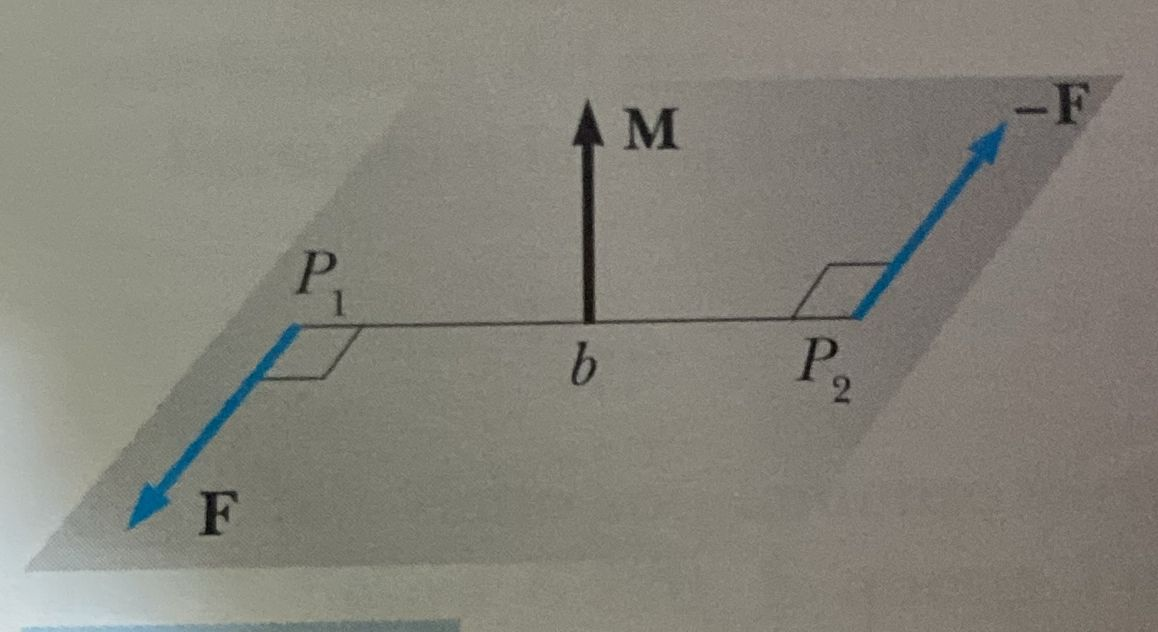
\includegraphics[width=\linewidth]{coppiaDiForze.jpeg}}
\end{minipage}%
\hfill
\begin{minipage}[t]{0.55\textwidth}
  \raggedright
\textbf{Il momento dipende dal polo, a meno che non sia R=0}. Un'applicazione importante di questo risultato riguarda la \textbf{coppia di forze}. Si chiama così un sistema formato da due forze eguali e di verso opposto, aventi in generale diversa retta di azione. La distanza tra le due rette d'azione è chiamata \textbf{braccio della coppia, b}. La risultante delle due forze è nulla e pertanto il momento M non dipende dalla scelta del polo. M è ortogonale al piano individuato dalle due rette di azione, ha verso determinato dalla solita regola del prodotto vettoriale e modulo bF, come si ottiene scegliendo $P_2$ come polo.

\end{minipage}
Dato un sistema di forze applicate in punti diversi e fissato un polo per i momenti, con il che sono noti R e $M_0$, questo sistema può essere sempre ridotto a una forza R con retta d'azione passante per il polo (così il momento di R rispetto al polo è nullo) e ad una coppia di forze di momento $M_0$ (che ha risultante nulla e momento indipendente dal polo).
\subsubsection{Sistema di forze parallele}
\begin{minipage}[t]{0.4\textwidth}
  \raisebox{-\height}{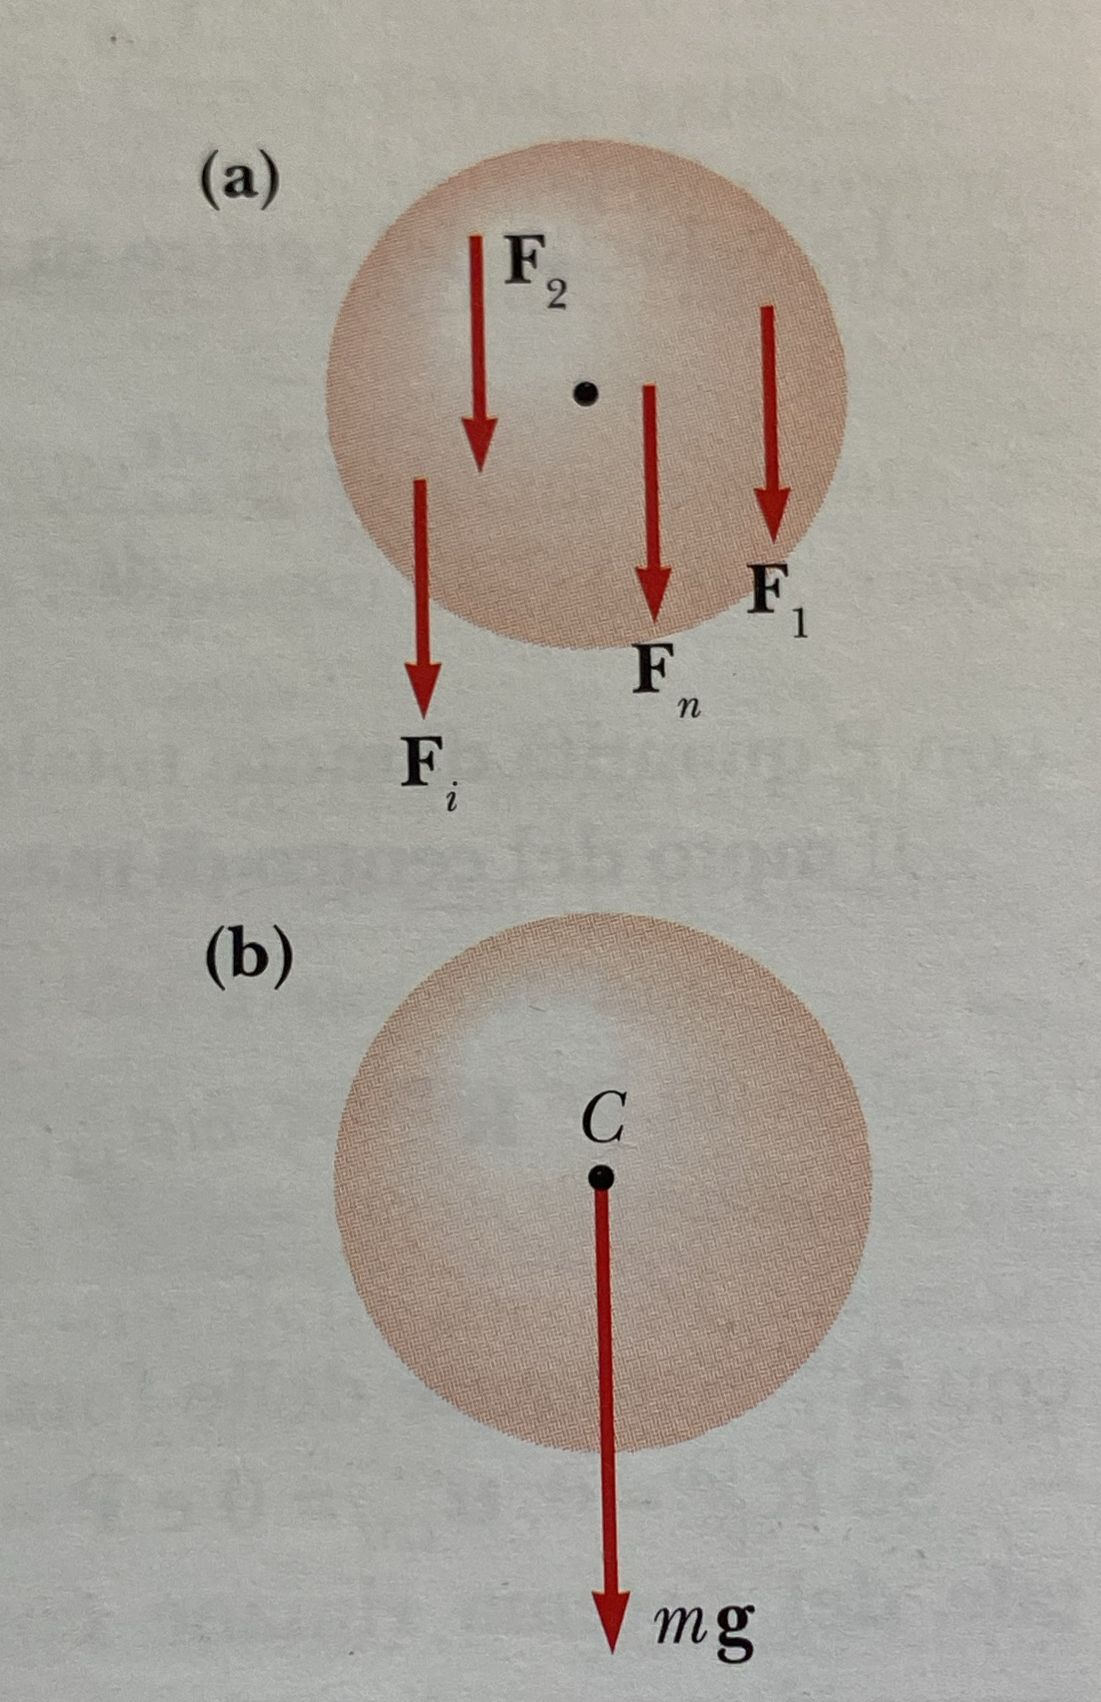
\includegraphics[width=\linewidth]{SistemaDiForzeParallele.jpeg}}
\end{minipage}%
\hfill
\begin{minipage}[t]{0.55\textwidth}
  \raggedright
Tale sistema, è formato da forze aventi tutte la stessa direzione, individuata dal versore u. Di conseguenza la risultante R risulta parallela a u. Troviamo:
\begin{equation}
    \vec{r}_C=\vec{OC}=\frac{\sum_iF_i\vec{r}_i}{\sum_iF_i}
\end{equation}
Il punto C, individuato dal vettore $\vec{r}_C$, è chiamato \textbf{centro delle forze parallele}. A differenza del caso generale di forze con direzioni qualsiasi, un sistema di forze parallele può sempre essere ridotto a una sola forza, pari alla risultante R, applicata in C. Un sistema molto comune di forze parallele è quello delle forze peso, applicate a un insieme di punti. Le singole forze sono pari a $m_i\vec{g}$, la risultante è $\vec{R}=m\vec{g}$ e il centro è individuato dal vettore:
\begin{equation}
     \vec{r}_C=\frac{\sum_im_ig\vec{r}_i}{\sum_im_ig}=\frac{\sum_im_i\vec{r}_i}{\sum_im_i}=\vec{r}_{CM}
\end{equation}
Il centro delle forze peso, detto anche \textbf{centro di gravità o baricentro}, coincide con il centro di massa. Osserviamo che per poter considerare le forze peso parallele l'estensione del sistema non deve essere molto grande, così da poter trascurare la curvatura della terra. Il momento risultante delle forze peso è:
\begin{equation}
    \vec{M}=\vec{OC} \times m \vec{g}= \vec{r_{CM}} \times m \vec{g}
\end{equation}
\end{minipage}

\clearpage
\end{document}
